\documentclass[11pt,a4paper,oneside,english]{report}

  %% Include packages and settings
  %\frenchspacing
\usepackage{babel}
\usepackage[utf8]{inputenc}
\usepackage[T1]{fontenc}
%\usepackage[T1,mtbold,lucidacal,mtplusscr,subscriptcorrection]{mathtime}
\usepackage{times}
\usepackage[pdftex]{graphicx}
\usepackage{color}
%\usepackage{palatino}
\usepackage[pdftex,colorlinks=true,citecolor=black,bookmarks=true,
            pagecolor=black,linkcolor=black,menucolor=black,
            urlcolor=black]{hyperref}
\usepackage{amsmath,amsfonts,amssymb}
\usepackage[small,bf,up,margin=10pt]{caption} % Changes caption appearence
\usepackage{eufrak}
\usepackage{amsbsy}
\usepackage{eucal}
\usepackage{subfigure}
\usepackage{longtable}
\usepackage{url}
\RequirePackage{moreverb}
\RequirePackage{listings}
\urlstyle{same}
\usepackage[authoryear,round]{natbib}
\bibliographystyle{apalike}

\lstloadlanguages{[visual]C++,matlab}
\lstset{basicstyle=\normalsize,columns=fullflexible,frame=lines}

% Fix overflow
\pretolerance=150
\tolerance=150
\setlength{\emergencystretch}{3em}

% Orphan control
\widowpenalty=1000
\clubpenalty=1000
\raggedbottom


% Matlab code syntax highlight
\usepackage[framed]{mcode}
%\renewenvironment{verbatim}{\begin{lstlisting}}{\end{lstlisting}}

% Set cover background picture
\usepackage{eso-pic}
  \newcommand\BackgroundPic{
    \put(0,0){
    \parbox[b][\paperheight]{\paperwidth}{%
    \vfill
    \centering
    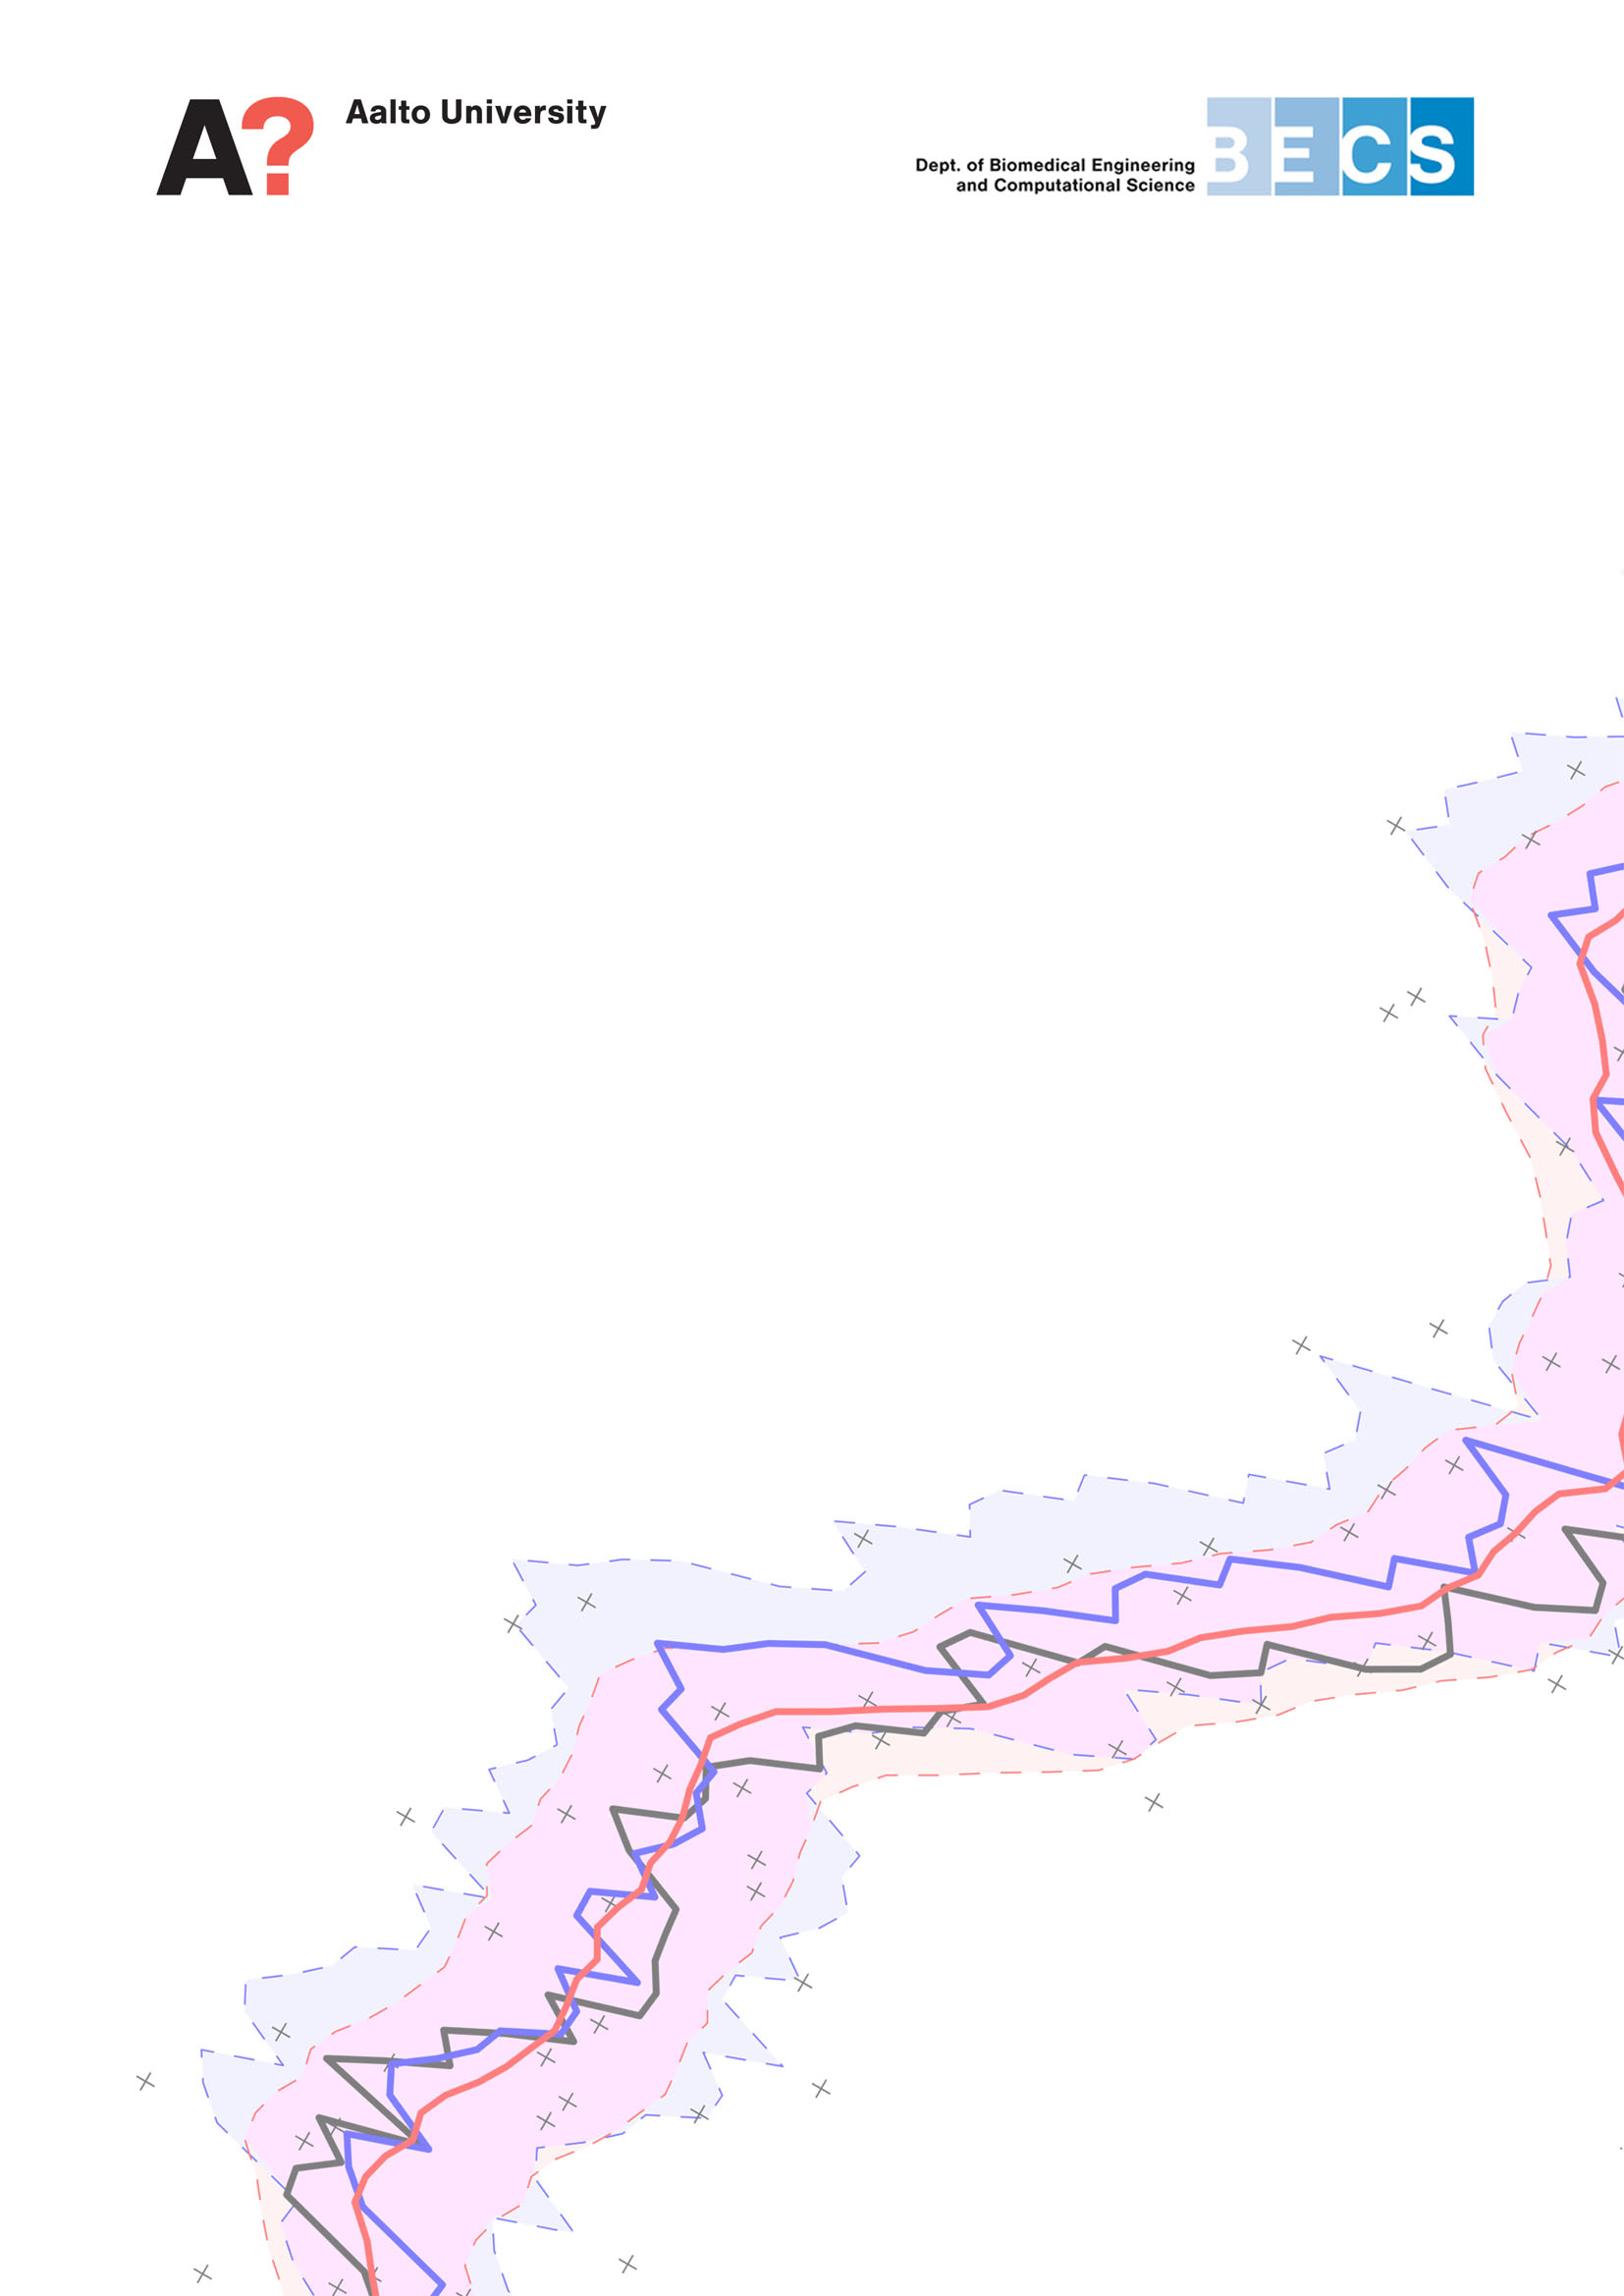
\includegraphics[width=\paperwidth,height=\paperheight,
      keepaspectratio]{pics/cover}%
    \vfill
  }}}



%\oddsidemargin 1cm    %   Note \oddsidemargin = \evensidemargin
%\evensidemargin 1cm
%\marginparwidth 0.2 true cm
%\topmargin -1.25cm
%\addtolength{\headsep}{0.25in}
%\textheight 21.5 true cm       % Height of text (including footnotes & figures)
%\textwidth 14 true cm        % Width of text line.

\usepackage{multirow}

% Headers
\usepackage{fancyhdr}
\pagestyle{fancy}
%\lhead{\textit{B.Sc. thesis draft \today}}
\lhead{\footnotesize \textsf \leftmark}
\chead{}
\rhead{}
\lfoot{}
\cfoot{\thepage}
\rfoot{}
\renewcommand{\headrulewidth}{0.5mm}
%\renewcommand{\footrulewidth}{0.5mm}

\pdfinfo{            
          /Title      (EFK/UKF toolbox for Matlab)
          /Author     (Jouni Hartikainen, Arno Solin, Simo Särkkä)
          /Keywords   (Kalman filter Extended Unscented optimal filtering)
}


%\newtheorem{Lemma}{Lemma}
%\newtheorem{Definition}{Definition}
%\DeclareMathOperator{\Poisson}{Poisson}
%\DeclareMathOperator{\GP}{\mathcal{GP}}
%\DeclareMathOperator{\Kfu}{\mathbf{K}_{f,u}}
%\DeclareMathOperator{\Kuf}{\mathbf{K}_{u,f}}
%\DeclareMathOperator{\Kff}{\mathbf{K}_{f,f}}
%\DeclareMathOperator{\Kfa}{\mathbf{K}_{f,\ast}}
%\DeclareMathOperator{\Kaf}{\mathbf{K}_{\ast,f}}
%\DeclareMathOperator{\Kaa}{\mathbf{K}_{\ast,\ast}}
%\DeclareMathOperator{\Kuu}{\mathbf{K}_{u,u}}
%\DeclareMathOperator{\Kau}{\mathbf{K}_{\ast,u}}
%\DeclareMathOperator{\Qff}{\mathbf{Q}_{f,f}}
%\DeclareMathOperator{\Qaa}{\mathbf{Q}_{\ast,\ast}}
%\DeclareMathOperator{\Qfa}{\mathbf{Q}_{f,\ast}}
%\DeclareMathOperator{\Qaf}{\mathbf{Q}_{\ast,f}}
%\DeclareMathOperator{\x}{\mathbf{x}}
%\DeclareMathOperator{\f}{\mathbf{f}}
%\DeclareMathOperator{\y}{\mathbf{y}}
%\DeclareMathOperator{\uu}{\mathbf{u}}
%\DeclareMathOperator{\LL}{\mathbf{\Lambda}}
%\DeclareMathOperator{\bb}{\mathbf{b}}

%\newcommand{\bm}{\mathbf}

\providecommand\figurename{Figure}
\providecommand\tablename{Table}
\providecommand\partname{Part}
\providecommand\appendixname{Appendix}
\providecommand\equationname{Eq\-ua\-tion}
%\providecommand\Itemname{item}
\providecommand\chaptername{chapter}
%\providecommand\sectionname{section}
\providecommand\subsectionname{section}
\providecommand\subsubsectionname{section}
%\providecommand\paragraphname{paragraph}
%\providecommand\theoremname{Theorem}


%%%%%%%%%%%%%%%%%%%%%%%%%%%%%%%%%%%%%%%%%
%
% macros begin
%
%%%%%%%%%%%%%%%%%%%%%%%%%%%%%%%%%%%%%%%%%
\renewcommand{\vec}[1]{\mathbf{#1}}
\newcommand{\set}[1]{\mathcal{#1}}
\newcommand{\alg}[1]{\mathscr{#1}}
\newcommand{\spc}[1]{\mathbb{#1}}
\newcommand{\ope}[1]{\EuScript{#1}}
\newcommand{\mea}[1]{#1}

\renewcommand{\vec}[1]{\mathbf{#1}}
\newcommand{\mat}[1]{\mathbf{#1}}
%\renewcommand{\vec}[1]{#1}
%\newcommand{\mat}[1]{#1}
\newcommand{\V}[1]{\mathbf{#1}}


\newcommand{\diff}[0]{\mathrm{d}}
%\newcommand{\diff}[0]{d}
%\newcommand{\B}[0]{\mathrm{\beta}}
%\newcommand{\Dt}[0]{\partial t}
\newcommand{\Dt}[0]{\delta t}
\newcommand{\Dx}[0]{\delta \vec{x}}
\newcommand{\Eg}[0]{\EuScript{E}}
\newcommand{\T}[0]{\mathsf{^T}}

\newcommand{\vectheta}[0]{\boldsymbol{\theta}}
\newcommand{\vecalpha}[0]{\boldsymbol{\alpha}}
\newcommand{\vecbeta}[0]{\boldsymbol{\beta}}
\newcommand{\veceta}[0]{\boldsymbol{\eta}}
\newcommand{\vecmu}[0]{\boldsymbol{\mu}}
\newcommand{\vecsigma}[0]{\boldsymbol{\sigma}}

%\DeclareMathOperator{\tr}{trace}
\DeclareMathOperator{\tr}{tr}
\DeclareMathOperator{\diag}{diag}
\DeclareMathOperator{\chol}{chol}
\DeclareMathOperator{\dchol}{dchol}
\DeclareMathOperator{\Cov}{Cov}
\DeclareMathOperator{\Var}{Var}
\DeclareMathOperator{\E}{E}
\DeclareMathOperator{\N}{N}
\DeclareMathOperator{\gammad}{Gamma}
\DeclareMathOperator{\expd}{Exp}
\DeclareMathOperator{\sech}{sech}
\DeclareMathOperator{\dt}{\Delta t}
\DeclareMathOperator{\dtk}{\Delta t_k}


\newcommand{\balpha}[0]{\boldsymbol{\alpha}}
\newcommand{\bbeta}[0]{\boldsymbol{\beta}}
\newcommand{\btheta}[0]{\boldsymbol{\theta}}
\newcommand{\bphi}[0]{\boldsymbol{\phi}}
\newcommand{\bmu}[0]{\boldsymbol{\mu}}
\newcommand{\bSigma}[0]{\boldsymbol{\Sigma}}
\newcommand{\blambda}[0]{\boldsymbol{\lambda}}
\newcommand{\brho}[0]{\boldsymbol{\rho}}
\newcommand{\bGamma}[0]{\boldsymbol{\Gamma}}

%\newtheorem{example}{Example}[section]
%\newtheorem{definition}{Definition}[section]
%\newtheorem{theorem}{Theorem}[section]
%\newtheorem{lemma}{Lemma}[section]
%\newtheorem{corollary}{Corollary}[section]
%\newtheorem{property}{Property}[section]

%\newtheorem{algorithm}{Algorithm}[chapter]
%\newtheorem{example}{Example}[chapter]
%\newtheorem{definition}{Definition}[chapter]
%\newtheorem{theorem}{Theorem}[chapter]
%\newtheorem{lemma}{Lemma}[chapter]
%\newtheorem{corollary}{Corollary}[chapter]
%\newtheorem{property}{Property}[chapter]
%\newtheorem{remark}{Remark}[chapter]

%%%%%%%%%%%%%%%%%%%%%%%%%%%%%%%%%%%%%%%%%
%
% macros end
%
%%%%%%%%%%%%%%%%%%%%%%%%%%%%%%%%%%%%%%%%%

% Lists
\newenvironment{boxlist1}{
  \begin{list}{}{\leftmargin=2pt}}{ % \leftmargin=0pt,
    % $\bullet$  ,\parsep=0pt
  \end{list}}
\newenvironment{boxlist2}{
  \begin{list}{-}{\itemsep=-1pt,\topsep=0pt,\setlength{\leftmargin}{8pt}}}{
    % 
  \end{list}}

\title{{\Huge Optimal Filtering \\with Kalman Filters and Smoothers} \\
  a Manual for the Matlab toolbox EKF/UKF \\
  {\normalsize Version~1.3}}

\author{Jouni Hartikainen, Arno Solin, and Simo Särkkä\\
Department of Biomedical Engineering and Computational Science,\\
Aalto University School of Science,\\
P.O.Box 1100, FI-00076 AALTO, Espoo, Finland \\
{\it jouni.hartikainen@aalto.fi, arno.solin@aalto.fi, simo.sarkka@aalto.fi}\vspace{-.5\baselineskip}}
%\date{}


\newenvironment{demo1}{\noindent\textbf{demo\_2input:}\begin{quote}\small\itshape}
{\end{quote}}

\newenvironment{example}{\small\begin{verbatim}}
{\end{verbatim}}

\newenvironment{demo2}{\noindent\textbf{demo\_2ingp:}\begin{quote}\small\itshape}
{\end{quote}}





\begin{document}

\AddToShipoutPicture*{\BackgroundPic}
\maketitle

\begin{abstract}

  In this paper we present a documentation for an optimal filtering
  toolbox for the mathematical software package Matlab. 
  The toolbox features many filtering methods for discrete-time 
  state space models, including the well-known linear Kalman filter 
  and several non-linear extensions to it. 
  These non-linear methods are the extended Kalman filter, 
  the unscented Kalman filter, the Gauss-Hermite Kalman filter and 
  the third-order symmetric cubature Kalman filter. Algorithms for
  multiple model systems are provided in the form of an Interacting
  Multiple Model (IMM) filter and it's non-linear extensions, which
  are based on banks of extended and unscented Kalman filters. Also
  included in the toolbox are the Rauch-Tung-Striebel and two-filter
  smoother counter-parts for the filters, which can be used to smooth
  the previous state estimates, after obtaining new measurements. The
  usage and function of each method is illustrated with eight
  demonstration problems.

\end{abstract}


%---------------------------------------
\newpage

\tableofcontents

\newpage
%---------------------------------------

\section*{Preface}

Most of the software provided with this toolbox were originally created
by Simo Särkkä while he was doing research on his doctoral thesis
\citep{Sarkka:2006} in the Laboratory of Computational Engineering (LCE)
at Helsinki University of Technology (HUT). This document has been
written by Jouni Hartikainen at LCE during spring 2007 with a little
help from Simo Särkkä. Jouni also checked and commented the software
code thoroughly. Many (small) bugs were fixed, and also some new
functions were implemented (for example 2nd order EKF and augmented
form UKF). Jouni also provided the software code for first three
demonstrations, modified the two last ones a bit, and ran all the
simulations. In 2010, Arno Solin added the cubature integration based 
methods to the toolbox.

First author would like to thank Doc. Aki Vehtari for helpful comments
during the work and for coming up with the idea of this toolbox in the
first place. Prof. Jouko Lampinen also deserves thanks for ultimately
making this work possible.

\newpage

%%%%%%%%%%%%%%%%%%%%%%%%%%%%%%%%%%%%%%%%%%%%%%%%%%%%%%%%%%%%%%%%%%%%%%%%%%%%%%
%
  %%%%%%%%%%%%%%%%%%%%%%%%%%%%%%%%%%%%%%%%%%%%%%%%%%%%%%%%%%%%%%%%%%%%%%%%%%%%%%
%
\chapter{Introduction}
%
%%%%%%%%%%%%%%%%%%%%%%%%%%%%%%%%%%%%%%%%%%%%%%%%%%%%%%%%%%%%%%%%%%%%%%%%%%%%%%

The term optimal filtering refers to methodology used for estimating
the {\it state} of a time varying system, from which we observe
indirect noisy measurements. The state refers to the physical state,
which can be described by dynamic variables, such as position,
velocity and acceleration of a moving object. The noise in the
measurements means that there is a certain degree of uncertainty in
them.  The dynamic system evolves as a function of time, and there is
also noise in the dynamics of system, {\it process noise}, meaning
that the dynamic system cannot be modelled entirely deterministically.
In this context, the term filtering basically means the process of
filtering out the noise in the measurements and providing an optimal
estimate for the state given the observed measurements and the
assumptions made about the dynamic system.

This toolbox provides basic tools for estimating the state of a linear
dynamic system, the Kalman filter, and also two extensions for it, the
extended Kalman filter (EKF) and unscented Kalman filter (UKF), both
of which can be used for estimating the states of nonlinear dynamic
systems. Also the smoother counterparts of the filters are provided.
Smoothing in this context means giving an estimate of the state of the
system on some time step given all the measurements including ones
encountered after that particular time step, in other words, the
smoother gives a smoothed estimate for the history of the system's
evolved state given all the measurements obtained so far.

This documentation is organized as follows: 
\begin{itemize}

\item First we briefly introduce the concept of discrete-time state
  space models. After that we consider linear, discrete-time state
  space models in more detail and review Kalman filter, which is the
  basic method for recursively solving the linear state space
  estimation problems. Also Kalman smoother is introduced. After that
  the function of Kalman filter and smoother and their usage in this
  toolbox in demonstrated with one example (CWPA-model).

\item Next we move from linear to nonlinear state space models and
  review the extended Kalman filter (and smoother), which is the
  classical extension to Kalman filter for nonlinear estimation. The
  usage of EKF in this toolbox is illustrated exclusively with one
  example (Tracking a random sine signal), which also compares the
  performances of EKF, UKF and their smoother counter-parts.

\item After EKF we review unscented Kalman filter (and smoother),
  which is a newer extension to traditional Kalman filter to cover
  nonlinear filtering problems. The usage of UKF is illustrated with
  one example (UNGM-model), which also demonstrates the differences
  between different nonlinear filtering techniques.

\item We extend the concept of sigma-point filtering by studying
  other non-linear variants of Kalman filters. The Gauss-Hermite
  Kalman filter (GHKF) and third-order symmetric Cubature Kalman
  filter (CKF) are presented at this stage.

\item To give a more thorough demonstration to the provided methods
  two more classical nonlinear filtering examples are provided
  (Bearings Only Tracking and Reentry Vehicle Tracking).

\item In chapter~\ref{ch:IMM} we shortly review the concept multiple model
  systems in general, and in sections~\ref{ch:IMM}.1 and \ref{ch:IMM}.2 we take a look at
  linear and non-linear multiple model systems in more detail. We also
  review the standard method, the Interacting Multiple Model (IMM)
  filter, for estimating such systems. It's usage and function is
  demonstrated with three examples.

%\item Lastly we list and describe briefly all the functions included
%  in the toolbox.

\end{itemize}

Details of the toolbox functions can be found on the toolbox web page, or in
Matlab by typing \texttt{help <function name>}. The mathematical notation used in this document follows the notation used in \citep{Sarkka:2006}.



%
%%%%%%%%%%%%%%%%%%%%%%%%%%%%%%%%%%%%%%%%%%%%%%%%%%%%%%%%%%%%%%%%%%%%%%%%%%%%%%

\clearpage
\newpage



%%%%%%%%%%%%%%%%%%%%%%%%%%%%%%%%%%%%%%%%%%%%%%%%%%%%%%%%%%%%%%%%%%%%%%%%%%%%%%
%
  %%%%%%%%%%%%%%%%%%%%%%%%%%%%%%%%%%%%%%%%%%%%%%%%%%%%%%%%%%%%%%%%%%%%%%%%%%%%%%
%
\chapter{Discrete-Time State Space Models: \\ Linear Models}
\label{ch:Linear-models}
%
%%%%%%%%%%%%%%%%%%%%%%%%%%%%%%%%%%%%%%%%%%%%%%%%%%%%%%%%%%%%%%%%%%%%%%%%%%%%%%

\section{Discrete-Time State Space Models}

In this section we shall consider models where the states are defined
on discrete time instances. The models are defined recursively in
terms of distributions
%
\begin{equation}
\begin{split}
    \vec{x}_k &\sim p(\vec{x}_k\,|\,\vec{x}_{k-1}) \\
    \vec{y}_k &\sim p(\vec{y}_k\,|\,\vec{x}_k),
\end{split}
\label{eq:dss_model}
\end{equation}
%
where
%
\begin{itemize}
\item $\vec{x}_k \in \spc{R}^n$ is the {\em state} of the system on
  the time step $k$.
  
\item $\vec{y}_k \in \spc{R}^m$ is the measurement on the time step $k$.

\item $p(\vec{x}_k\,|\,\vec{x}_{k-1})$ is the dynamic model which
charaterizes the dynamic behaviour of the system. Usually the model is
a probability density (continous state), but it can also be a counting
measure (discrete state), or a combination of them, if the state is
both continuous and discrete.
%
\item $p(\vec{y}_k\,|\,\vec{x}_k)$ is the model for measurements,
which describes how the measurements are distributed given the
state. This model characterizes how the dynamic model is perceived by
the observers.
\end{itemize}

A system defined this way has the so called \emph{Markov}-property,
which means that the state $\vec{x}_k$ given $\vec{x}_{k-1}$ is
independent from the history of states and measurements, which can
also be expressed with the following equality:
%
\begin{equation} p(\vec{x}_k\,|\,\vec{x}_{1:k-1},\vec{y}_{1:k-1}) =
p(\vec{x}_k\,|\,\vec{x}_{k-1}).
\end{equation}
%
The past doesn't depend on the future given the present, which is the
same as
%
\begin{equation} p(\vec{x}_{k-1}\,|\,\vec{x}_{k:T},\vec{y}_{k:T}) =
p(\vec{x}_{k-1}\,|\,\vec{x}_{k}).
\end{equation}
% 
The same applies also to measurements meaning that the measurement
$\vec{y}_k$ is independent from the histories of measurements and
states, which can be expressed with equality
%
\begin{equation} p(\vec{y}_k\,|\,\vec{x}_{1:k},\vec{y}_{1:k-1}) =
p(\vec{y}_k\,|\,\vec{x}_{k}).
\end{equation}


In actual application problems, we are interested in predicting and
estimating dynamic system's state given the measurements obtained so
far. In probabilistic terms, we are interested in the predictive
distribution for the state at the next time step
%
\begin{equation} p(\vec{x}_{k}\,|\,\vec{y}_{1:k-1}),
\end{equation}
%
and in the marginal posterior distribution for the state at the
current time step
%
\begin{equation} p(\vec{x}_{k}\,|\,\vec{y}_{1:k}).
\end{equation}
%
The formal solutions for these distribution are given by the following
recursive Bayesian filtering equations  \citep[e.g.][]{Sarkka:2006b}:
%
\begin{equation} p(\vec{x}_k\,|\,\vec{y}_{1:k-1}) = \int
p(\vec{x}_k\,|\,\vec{x}_{k-1}) \, p(\vec{x}_{k-1}\,|\,\vec{y}_{1:k-1})
\, \diff\vec{x}_{k-1}
\label{eq:bayesf_p}
\end{equation} and
\begin{equation} p(\vec{x}_k\,|\,\vec{y}_{1:k}) = \frac{1}{Z_k}
p(\vec{y}_k\,|\,\vec{x}_k) \, p(\vec{x}_k\,|\,\vec{y}_{1:k-1}),
\label{eq:bayesf_u}
\end{equation} where the normalization constant $Z_k$ is given as
 %
\begin{equation} Z_k = \int p(\vec{y}_k\,|\,\vec{x}_k) \,
p(\vec{x}_k\,|\,\vec{y}_{1:k-1}) \, \diff\vec{x}_k.
\label{eq:zk}
\end{equation}
%

In many cases we are also interested in smoothed state estimates of
previous time steps given the measurements obtained so far. In other
words, we are interested in the marginal posterior distribution
%
\begin{equation} p(\vec{x}_{k}\,|\,\vec{y}_{1:T}),
\end{equation}
%
where $T > k$. As with the filtering equations above also in this case
we can express the formal solution as a set of recursive Bayesian
equations \citep[e.g.][]{Sarkka+Vehtari+Lampinen:2007}:
%
\begin{equation}
\begin{split} p(\vec{x}_{k+1}\,|\,\vec{y}_{1:k}) &= \int
p(\vec{x}_{k+1}\,|\,\vec{x}_k) \, p(\vec{x}_k\,|\,\vec{y}_{1:k}) \,
\diff\vec{x}_k \\ p(\vec{x}_k\,|\,\vec{y}_{1:T}) &=
p(\vec{x}_k\,|\,\vec{y}_{1:k}) \int \left[
\frac{p(\vec{x}_{k+1}\,|\,\vec{x}_k) \,
p(\vec{x}_{k+1}\,|\,\vec{y}_{1:T})}
{p(\vec{x}_{k+1}\,|\,\vec{y}_{1:k})} \right] \diff \vec{x}_{k+1}.
\end{split}
\end{equation}
%





%The formal solutions for these marginal distributions are not described here, 
%but interested readers should see, for example, (Särkkä, 2006b) for more details.

%%%%%%%%%%%%%%%%%%%%%%%%%%%%%%%%%%%%%%%%%%%%%%%%%%%%%%%%%%%%%%%%%%%%%%%%%%%%%%
%
\section{Linear State Space Estimation}
%
%%%%%%%%%%%%%%%%%%%%%%%%%%%%%%%%%%%%%%%%%%%%%%%%%%%%%%%%%%%%%%%%%%%%%%%%%%%%%%

The simplest of the state space models considered in this
documentation are linear models, which can be expressed with equations
of the following form:
%
\begin{equation}
\begin{split} \vec{x}_{k} &= \mat{A}_{k-1} \, \vec{x}_{k-1} +
\vec{q}_{k-1} \\ \vec{y}_{k} &= \mat{H}_{k} \, \vec{x}_{k} +
\vec{r}_{k},
\end{split}
\label{eq:kalman_model}
\end{equation}
%
where
%
\begin{itemize}
\item $\vec{x}_k \in \spc{R}^n$ is the {\em state} of the system on
the time step $k$.
%
\item $\vec{y}_k \in \spc{R}^m$ is the measurement on the time step
$k$.
%
\item $\vec{q}_{k-1} \sim \N(\vec{0},\mat{Q}_{k-1})$ is the process
noise on the time step $k-1$.
%
\item $\vec{r}_{k} \sim \N(\vec{0},\mat{R}_{k})$ is the measurement
noise on the time step $k$.
%
\item $\mat{A}_{k-1}$ is the transition matrix of the dynamic model.
%
\item $\mat{H}_k$ is the measurement model matrix.
%
\item The prior distribution for the state is $\vec{x}_{0} \sim
\N(\vec{m}_0,\mat{P}_0)$, where parameters $\vec{m}_0$ and $\mat{P}_0$
are set using the information known about the system under the study.
%
\end{itemize}

The model can also be equivalently expressed in probabilistic terms
with distributions
%
\begin{equation}
\begin{split} p(\vec{x}_{k}\,|\,\vec{x}_{k-1}) &=
\N(\vec{x}_{k}\,|\,\mat{A}_{k-1} \, \vec{x}_{k-1}, \mat{Q}_{k-1}) \\
p(\vec{y}_{k}\,|\,\vec{x}_{k}) &= \N(\vec{y}_{k}\,|\,\mat{H}_{k} \,
\vec{x}_{k} , \mat{R}_{k}).
\end{split}
\label{eq:kalman_model2}
\end{equation}
 
%%%%%%%%%%%%%%%%%%%%%%%%%%%%%%%%%%%%%%%%%%%%%%%%%%%%%%%%%%%%%%%%%%%%%%%%%%%%%%
%
\subsection{Discretization of Continuous-Time Linear Time-Invariant Systems}
%
%%%%%%%%%%%%%%%%%%%%%%%%%%%%%%%%%%%%%%%%%%%%%%%%%%%%%%%%%%%%%%%%%%%%%%%%%%%%%%

Often many linear time-invariant models are described with
continous-time state equations of the following form:
%
\begin{equation}
%
\frac{d \vec{x}(t)}{d t} = \mat{F} \vec{x}(t) + \mat{L} \vec{w}(t),
%
\label{eq:lti_cont_model}
%
\end{equation}
%
where
%
\begin{itemize}
%
\item the initial conditions are $\vec{x}(0) \sim
\N(\vec{m}(0),\mat{P}(0))$,
%
\item $\mat{F}$ and $\mat{L}$ are constant matrices, which
characterize the behaviour of the model,
matrix $\mat{Q}_c$.
\item $\vec{w}(t)$ is a white noise process with a power spectral
density $\mat{Q}_c$.
%
\end{itemize}

To be able to use the Kalman filter defined in the next section the
model (\ref{eq:lti_cont_model}) must be discretized somehow, so that
it can be described with a model of the form
(\ref{eq:kalman_model}). The solution for the discretized matrices
$\mat{A}_k$ and $\mat{Q}_k$ can be given as \citep[see, e.g.,][]{Sarkka:2006b,
Bar-Shalom+Li+Kirubarajan:2001}.
%
\begin{align} \mat{A}_k &= \exp(\mat{F} \, \Delta t_k)
\label{eq:ode_ak} \\ \mat{Q}_k &= \int_{0}^{\Delta t_k} \exp( \mat{F}
\, (\Delta t_k - \tau)) \, \mat{L} \, \mat{Q}_c \, \mat{L}^T \, \exp(
\mat{F} \, (\Delta t_k - \tau))^T \diff \tau,
\label{eq:ode_qk}
\end{align}
%
where $\Delta t_k = t_{k+1} - t_k$ is the stepsize of the
discretization. In some cases the $\mat{Q}_k$ can be calculated
analytically, but in cases where it isn't possible, the matrix can
still be calculated efficiently using the following matrix fraction
decomposition:
%
%
  \begin{equation} \left( \begin{array}{c} \mat{C}_k \\ \mat{D}_k
  \end{array} \right) = \exp \left\{ \left( \begin{array}{cc} \mat{F}
& \mat{L} \, \mat{Q}_c \, \mat{L}^T \\ \mat{0} & -\mat{F}^T
  \end{array} \right) \Delta t_k \right\} \left( \begin{array}{c}
\mat{0} \\ \mat{I}
  \end{array} \right).
  \label{eq:noisy_ltisolution_cov1}
  \end{equation}
  %
The matrix $\mat{Q}_k$ is then given as $\mat{Q}_k = \mat{C}_k
\mat{D}_k^{-1}$.

In this toolbox the discretization can be done with the function
\texttt{lti\_disc}, which uses the
matrix fractional decomposition.

%%%%%%%%%%%%%%%%%%%%%%%%%%%%%%%%%%%%%%%%%%%%%%%%%%%%%%%%%%%%%%%%%%%%%%%%%%%%%%
%
\subsection{Kalman Filter}
%
%%%%%%%%%%%%%%%%%%%%%%%%%%%%%%%%%%%%%%%%%%%%%%%%%%%%%%%%%%%%%%%%%%%%%%%%%%%%%%

The classical Kalman filter was first introduced by Rudolph E. Kalman in his
seminal paper \citep{Kalman:1960}. The purpose of the discrete-time Kalman filter
is to provide the closed form recursive solution for estimation of linear discrete-time dynamic
systems, which can be described by equations of the form (\ref{eq:kalman_model}).

Kalman filter has two steps: the prediction step, where the next state of the
system is predicted given the previous measurements, and the update step, where
the current state of the system is estimated  given the measurement at that time
step. The steps translate to equations as follows \citep[see, e.g.,][for derivation]{Sarkka+Vehtari+Lampinen:2007,Bar-Shalom+Li+Kirubarajan:2001}:

\begin{itemize}
\item {\em Prediction:}
%
\begin{equation}
\begin{split}
  \vec{m}^-_{k} &= \mat{A}_{k-1} \, \vec{m}_{k-1} \\
  \mat{P}^-_{k} &= \mat{A}_{k-1} \, \mat{P}_{k-1} \, \mat{A}_{k-1}^T
                 + \mat{Q}_{k-1}.
\end{split}
\label{eq:dkf_predict}
\end{equation}
%
\item {\em Update:} 
%
\begin{equation}
\begin{split}
  \vec{v}_{k} &= \vec{y}_k - \mat{H}_{k} \, \vec{m}^-_{k} \\
  \vec{S}_{k} &= \mat{H}_{k} \, \mat{P}^-_{k} \, \mat{H}_{k}^T + \vec{R}_{k} \\
  \vec{K}_{k} &= \mat{P}^-_{k} \, \mat{H}^T_{k} \, \vec{S}^{-1}_{k} \\
  \vec{m}_{k} &= \vec{m}^-_{k} + \vec{K}_{k} \, \vec{v}_k \\
  \mat{P}_{k} &= \mat{P}^-_{k} - \vec{K}_{k} \, \vec{S}_{k} \, \vec{K}^T_{k}, \\
\end{split}
\label{eq:dkf_update}
\end{equation}
\end{itemize}
%
where
%
\begin{itemize}
%
\item $\vec{m}^-_{k}$ and $\mat{P}^-_{k}$ are the predicted mean and covariance of the state,
respectively,  on the time step $k$ before seeing the measurement.
%
\item $\vec{m}_{k}$ and $\mat{P}_{k}$ are the estimated mean and covariance of
the state, respectively, on time step $k$ after seeing the measurement.

\item $\vec{v}_k$ is the innovation or the measurement residual on time step $k$.
%
\item $\mat{S}_k$ is the measurement prediction covariance on the time step $k$.
%
\item $\mat{K}_k$ is the filter gain, which tells how much the predictions should be corrected on time step $k$.
%
\end{itemize}
%
Note that in this case the predicted and estimated state covariances on different time steps do not
depend on any measurements, so that they could be calculated off-line before making any measurements
provided that the matrices $\mat{A}$, $\mat{Q}$, $\mat{R}$ and $\mat{H}$ are known on those
particular time steps. Usage for this property, however, is not currently provided explicitly
with this toolbox.

It is also possible to predict the state of system as many steps ahead as wanted just by looping
the predict step of Kalman filter, but naturally the accuracy of the estimate decreases with every
step.

The prediction and update steps can be calculated with functions \texttt{kf\_predict}
and \texttt{kf\_update}.

\subsection{Kalman Smoother}

The discrete-time Kalman smoother, also known as the Rauch-Tung-Striebel-smoother (RTS), 
\citep{Rauch+Tung+Striebel:1965,Gelb:1974,Bar-Shalom+Li+Kirubarajan:2001} can be used for computing
the smoothing solution for the model (\ref{eq:kalman_model}) given as distribution
%
\begin{equation}
  p(\vec{x}_{k}\,|\,\vec{y}_{1:T}) =
    \N(\vec{x}_{k}\,|\,\vec{m}^s_{k},\mat{P}^s_{k}).
\end{equation}
%
The mean and covariance $\vec{m}^s_{k}$ and $\mat{P}^s_{k}$ are calculated with the following equations:
%
\begin{equation}
\begin{split}
    \vec{m}^-_{k+1} &= \mat{A}_k \, \vec{m}_k  \\
    \mat{P}^-_{k+1} &= \mat{A}_k \, \mat{P}_k \, \mat{A}_k^T + \mat{Q}_k \\
    \vec{C}_{k} &= \mat{P}_k \, \mat{A}_k^T \, [\mat{P}^-_{k+1}]^{-1} \\
    \vec{m}^s_k &= \vec{m}_k
    + \mat{C}_k \, [\vec{m}^s_{k+1} - \vec{m}^-_{k+1}] \\
    \mat{P}^s_k &= \mat{P}_k
    + \mat{C}_k \, [\mat{P}^s_{k+1} - \mat{P}^-_{k+1}] \, \mat{C}^T_k,
\end{split}
\label{eq:kfrts}
\end{equation}
%
where
%
\begin{itemize}
%
\item $\vec{m}^s_k$ and $\mat{P}^s_k$ are the smoother estimates for the state mean and state
covariance on time step $k$.
%
\item $\vec{m}_k$ and $\mat{P}_k$ are the filter estimates for the state mean and state 
covariance on time step $k$.
%
\item $\vec{m}^-_{k+1}$ and $\mat{P}^-_{k+1}$ are the predicted state mean and state covariance
on time step $k+1$, which are the same as in the Kalman filter.
%
\item $\mat{C}_k$ is the smoother gain on time step $k$, which tells how much the smooted estimates
should be corrected on that particular time step.
%
\end{itemize}
%
The difference between Kalman filter and Kalman smoother is that the recursion in filter moves
forward and in smoother backward, as can be seen from the equations above. In smoother the recursion
starts from the last time step T with $\vec{m}^s_T = \vec{m}_T$ and $\mat{P}^s_T = \mat{P}_T$. 

The smoothed estimate for states and covariances using the RTS smoother can be
calculated with the function \texttt{rts\_smooth}.

In addition to RTS smoother it is possible to formulate the smoothing operation as a combination
of two optimum filters \citep{Fraser+Potter:1969}, of which the first filter sweeps the data forward going from the first measurement towards the last one, and the second sweeps backwards towards the opposite direction.

It can be shown, that combining the estimates produced by these two filters in a suitable way produces an smoothed estimate for the state, which has lower mean square error than any of these two filters alone \citep{Gelb:1974}. With linear models the forward-backward smoother gives the same error as the RTS-smoother, but in non-linear cases the error behaves differently in some
situations. In this toolbox forward-backward smoothing solution can be
calculated with function \texttt{tf\_smooth}.


%%%%%%%%%%%%%%%%%%%%%%%%%%%%%%%%%%%%%%%%%%%%%%%%%%%%%%%%%%%%%%%%%%%%%%%%%%%%%%
%
\subsection{Demonstration: 2D CWPA-model}
%
%%%%%%%%%%%%%%%%%%%%%%%%%%%%%%%%%%%%%%%%%%%%%%%%%%%%%%%%%%%%%%%%%%%%%%%%%%%%%%

Let's now consider a very simple case, where we track an object moving
in two dimensional space with a sensor, which gives measurements of
target's position in cartesian coordinates $x$ and $y$. In addition to
position target also has state variables for its velocities and accelerations toward both coordinate
axes, $\dot{x}$, $\dot{y}$, $\ddot{x}$ and $\ddot{y}$. In other words, the state of a
moving object on time step $k$ can be expressed as a vector
%
\begin{equation}
\vec{x}_k = 
\begin{pmatrix}
x_k & y_k & \dot{x}_k & \dot{y}_k & \ddot{x}_k & \ddot{y}_k
\end{pmatrix}^T.
%
\end{equation}
%
In continuous case the dynamics of the target's motion can be modelled as a linear, time-invariant system
%
\begin{equation}
%
\frac{d \vec{x}(t)}{dt} = \underbrace{\begin{pmatrix}
0 & 0 & 1 & 0 & 0 & 0 \\
0 & 0 & 0 & 1 & 0 & 0 \\
0 & 0 & 0 & 0 & 1 & 0 \\
0 & 0 & 0 & 0 & 0 & 1 \\
0 & 0 & 0 & 0 & 0 & 0 \\
0 & 0 & 0 & 0 & 0 & 0 
\end{pmatrix}}_{\mat{F}} \vec{x}(t)
+
\underbrace{\begin{pmatrix}
0 & 0 \\
0 & 0 \\
0 & 0 \\
0 & 0 \\
1 & 0 \\
0 & 1 \\
\end{pmatrix}}_{\mat{L}}\vec{w}(t), \label{eq:cwpa_cont_model}
%
\end{equation}
%
where $\vec{x}(t)$ is the target's state on the time $t$ and
$\vec{w}(t)$ is a white noise process with power spectral density
%
\begin{equation}
\mat{Q}_c = 
\begin{pmatrix}
q & 0 \\
0   & q
\end{pmatrix}
= 
\begin{pmatrix}
0.2 & 0 \\
0   & 0.2
\end{pmatrix}.
\end{equation}
%
As can be seen from the equation the acceleration of the object is perturbed with a white noise process and hence this model has the name continous Wiener process acceleration (CWPA) model. There is also other models similar to this, as for example the continous white noise acceleration (CWNA) model \citep{Bar-Shalom+Li+Kirubarajan:2001}, where the velocity is perturbed with a white noise process.

The measurement matrix is set to
%
\begin{equation}
%
\mat{H} = \begin{pmatrix}
1 & 0 & 0 & 0 & 0 & 0 \\
0 & 1 & 0 & 0 & 0 & 0 \\
\end{pmatrix},
%
\end{equation}
%
which means that the observe only the position of the moving object.
To be able to estimate this system with a discrete-time Kalman filter the differential equation defined
above must be discretized somehow to get a discrete-time state equation of the form (\ref{eq:kalman_model}). It
turns out, that the matrices $\mat{A}$ and $\mat{Q}$ can be calculated analytically with equations (\ref{eq:ode_ak})
and (\ref{eq:ode_qk}) to give the following:
%
\begin{align}
%
\mat{A}  = \begin{pmatrix}
1 & 0 & \dt & 0    & \frac{1}{2}\dt^2    & 0 \\
0 & 1 & 0    & \dt & 0    & \frac{1}{2}\dt^2\\
0 & 0 & 1    & 0    & \dt & 0 \\
0 & 0 & 0    & 1    & 0    & \dt \\
0 & 0 & 0    & 0    & 1    & 0 \\
0 & 0 & 0    & 0    & 0    & 1 \\ 
\end{pmatrix}  
\end{align}%
\begin{align}
\mat{Q}  =   \begin{pmatrix}
\frac{1}{20}\dt^5 & 0 & \frac{1}{8}\dt^4 & 0 & \frac{1}{6}\dt^3 & 0 \\
0 & \frac{1}{20}\dt^5 & 0 & \frac{1}{8}\dt^4 & 0 & \frac{1}{6}\dt^3 \\
\frac{1}{8}\dtk4 & 0 & \frac{1}{6}\dt^3 & 0 &\frac{1}{2}\dt^2  & 0 \\
0 & \frac{1}{8}\dt^4 & 0 & \frac{1}{6}\dt^3 & 0 & \frac{1}{2}\dt^2 \\
\frac{1}{6}\dt^3 & 0 & \frac{1}{2}\dt^2 & 0 & \dt & 0 \\
0 & \frac{1}{6}\dt^3 & 0 & \frac{1}{2}\dt^2 & 0 & \dt 
\end{pmatrix}q,
%
\end{align}
%
where the stepsize is set to $\dt = 0.5$. These matrices can also
calculated using the function \texttt{lti\_disc}
introduced in section $2.1$ with the following code line:
%
\begin{lstlisting}
[A,Q] = lti_disc(F,L,Qc,dt);
\end{lstlisting}
% 
where matrices \texttt{F} and \texttt{L} are assumed to contain the matrices from equation
(\ref{eq:cwpa_cont_model}). 

The object starts from origo with zero velocity and acceleration
and the process is simulated 50 steps. The variance for the measurements is set to
%
\begin{equation}
\mat{R} = \begin{pmatrix}
10 & 0  \\
0  & 10 \\
\end{pmatrix},
\end{equation}
%
which is relatively high so that the the difference between the filtering and
smoothing (described in next section) estimates becomes clearer. The real
position of the object and measurements of it are plotted in the figure
\ref{fig:example1_1}. 

\begin{figure}
\begin{center}
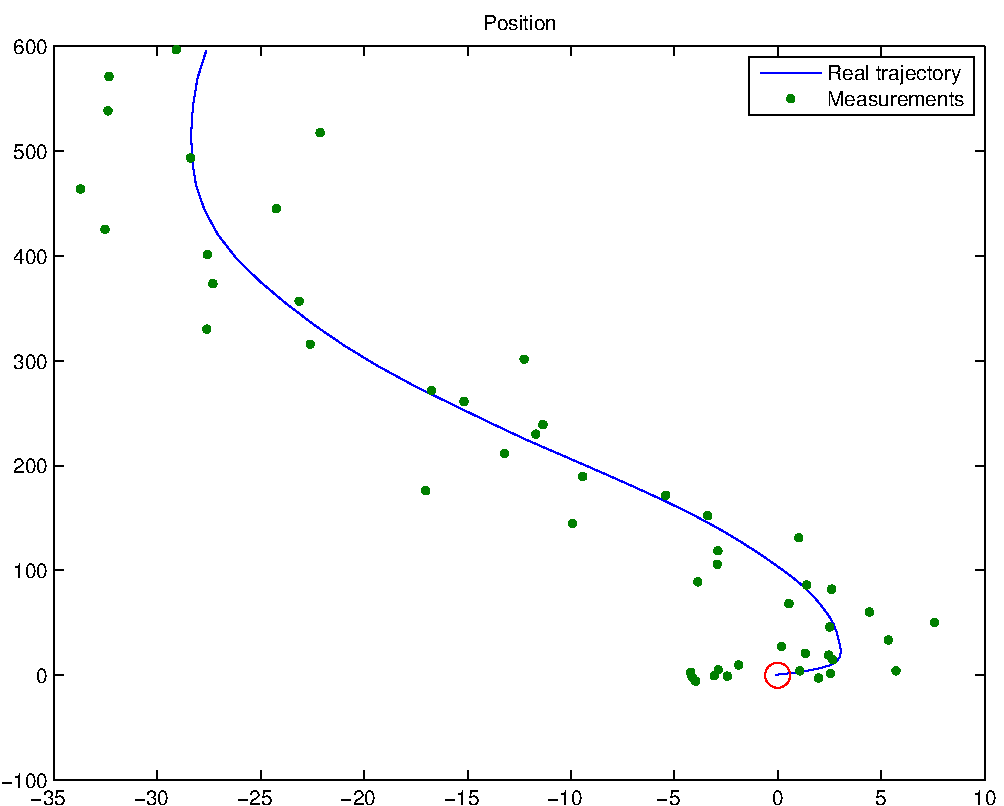
\includegraphics[width=0.7\textwidth]{pics/demo1_f1}
\caption{The real position of the moving object and the simulated
  measurements of it using the CWPA model. The circle marks the
  starting point of the object.}
\label{fig:example1_1}
\end{center}
\end{figure}

The filtering is done with the following code fragment:
%
\begin{lstlisting}
MM = zeros(size(m,1), size(Y,2));
PP = zeros(size(m,1), size(m,1), size(Y,2));

for i = 1:size(Y,2)
   [m,P] = kf_predict(m,P,A,Q);
   [m,P] = kf_update(m,P,Y(:,i),H,R);
   MM(:,i) = m;
   PP(:,:,i) = P;
end
\end{lstlisting}
%
In the first 2 lines the space for state mean and covariance estimates is
reserved, and the rest of the code contains the actual filtering loop, where
we make the predict and update steps of the Kalman filter. The variables
\texttt{m} and \texttt{P} are assumed to contain the initial guesses for the
state mean and covariance before reaching the for-statement. Variable
\texttt{Y} is assumed to contain the measurements made from the system
(See the full source code of the example (\texttt{kf\_cwpa\_demo.m}) provided with the toolbox
to see how we generated the measurements by simulating the dynamic system). In
the end of each iteration the acquired estimates are stored to matrices
\texttt{MM} and \texttt{PP}, for which we reserved space earlier. The estimates
for object's position and velocity with Kalman filter and are plotted in figure
\ref{fig:example1_2}.\\

%\begin{figure}
%\begin{center}
%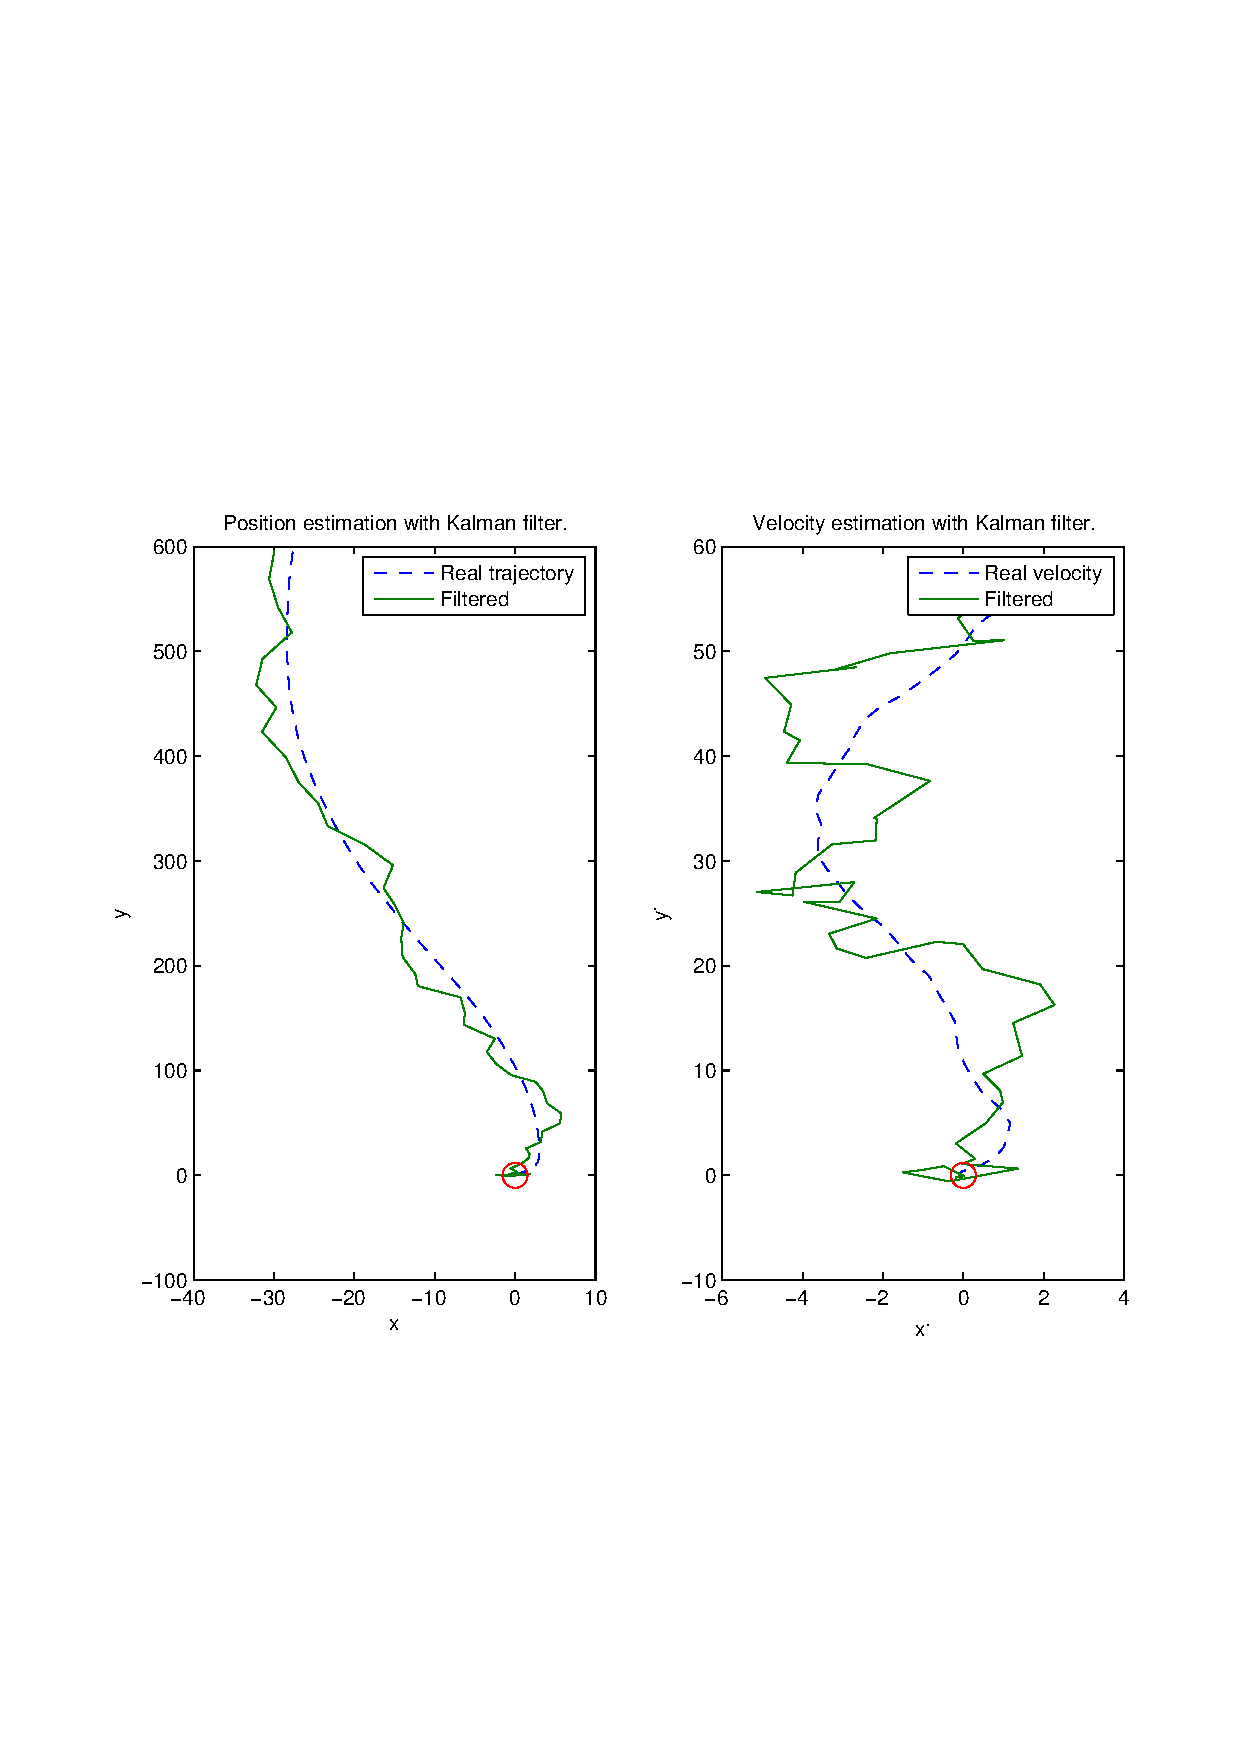
\includegraphics[width=11cm]{pics/demo1_f2}
%\caption{Estimates for position and velocity of the moving object
%  using the Kalman filter and CWPA model.}
%\label{fig:example1_2}
%\end{center}
%\end{figure}

The smoothed estimates for the state mean and covariance can be calculated with the
following code line:
%
\begin{lstlisting}
[SM,SP] = rts_smooth(MM,PP,A,Q);
\end{lstlisting}
%
The calculated smoothed estimates for object's position and velocity for the
earlier demonstration are plotted in figure \ref{fig:example1_3}. As expected
the smoother produces more accurate estimates than the filter as it uses all
measurements for the estimation each time step. Note that the difference between
the smoothed and filtered estimated would be smaller, if the measurements were
more accurate, as now the filter performs rather badly due to the great
uncertaintity in the measurements. The smoothing results of a
forward-backward smoother are not plotted here, as the result are
exactly the same as with the RTS smoother. 

As one would expect the estimates for object's velocity are clearly less
accurate than the estimates for the object's position as the positions are
observed directly and the velocities only indirectly. If the
velocities were also observed not only the velocity estimates would get
more accurate, but also the position ones as well. 

%\begin{figure}
%\begin{center}
%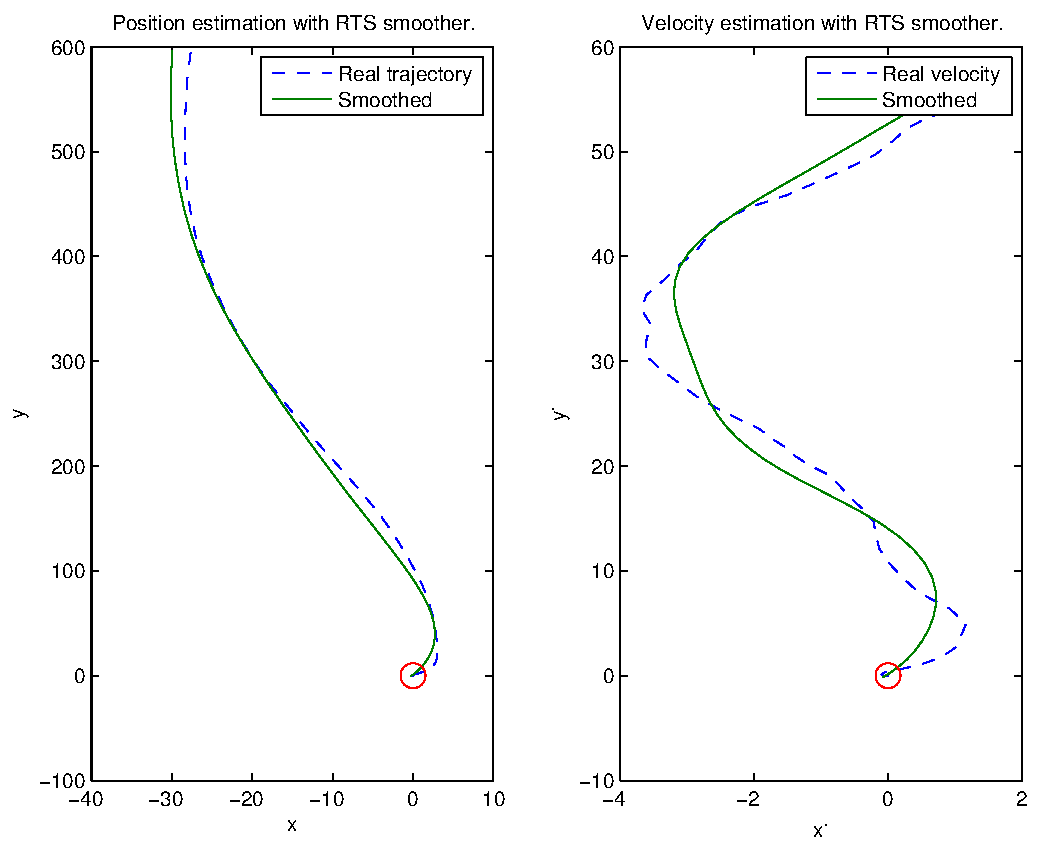
\includegraphics[width=11cm]{pics/demo1_f3}
%\caption{Estimate for position and velocity of the moving object using the RTS smoother and CWPA model.}
%\label{fig:example1_3}
%\end{center}
%\end{figure}




\begin{figure}[t]
 \centering
 \subfigure[Filter]{\label{fig:example1_2}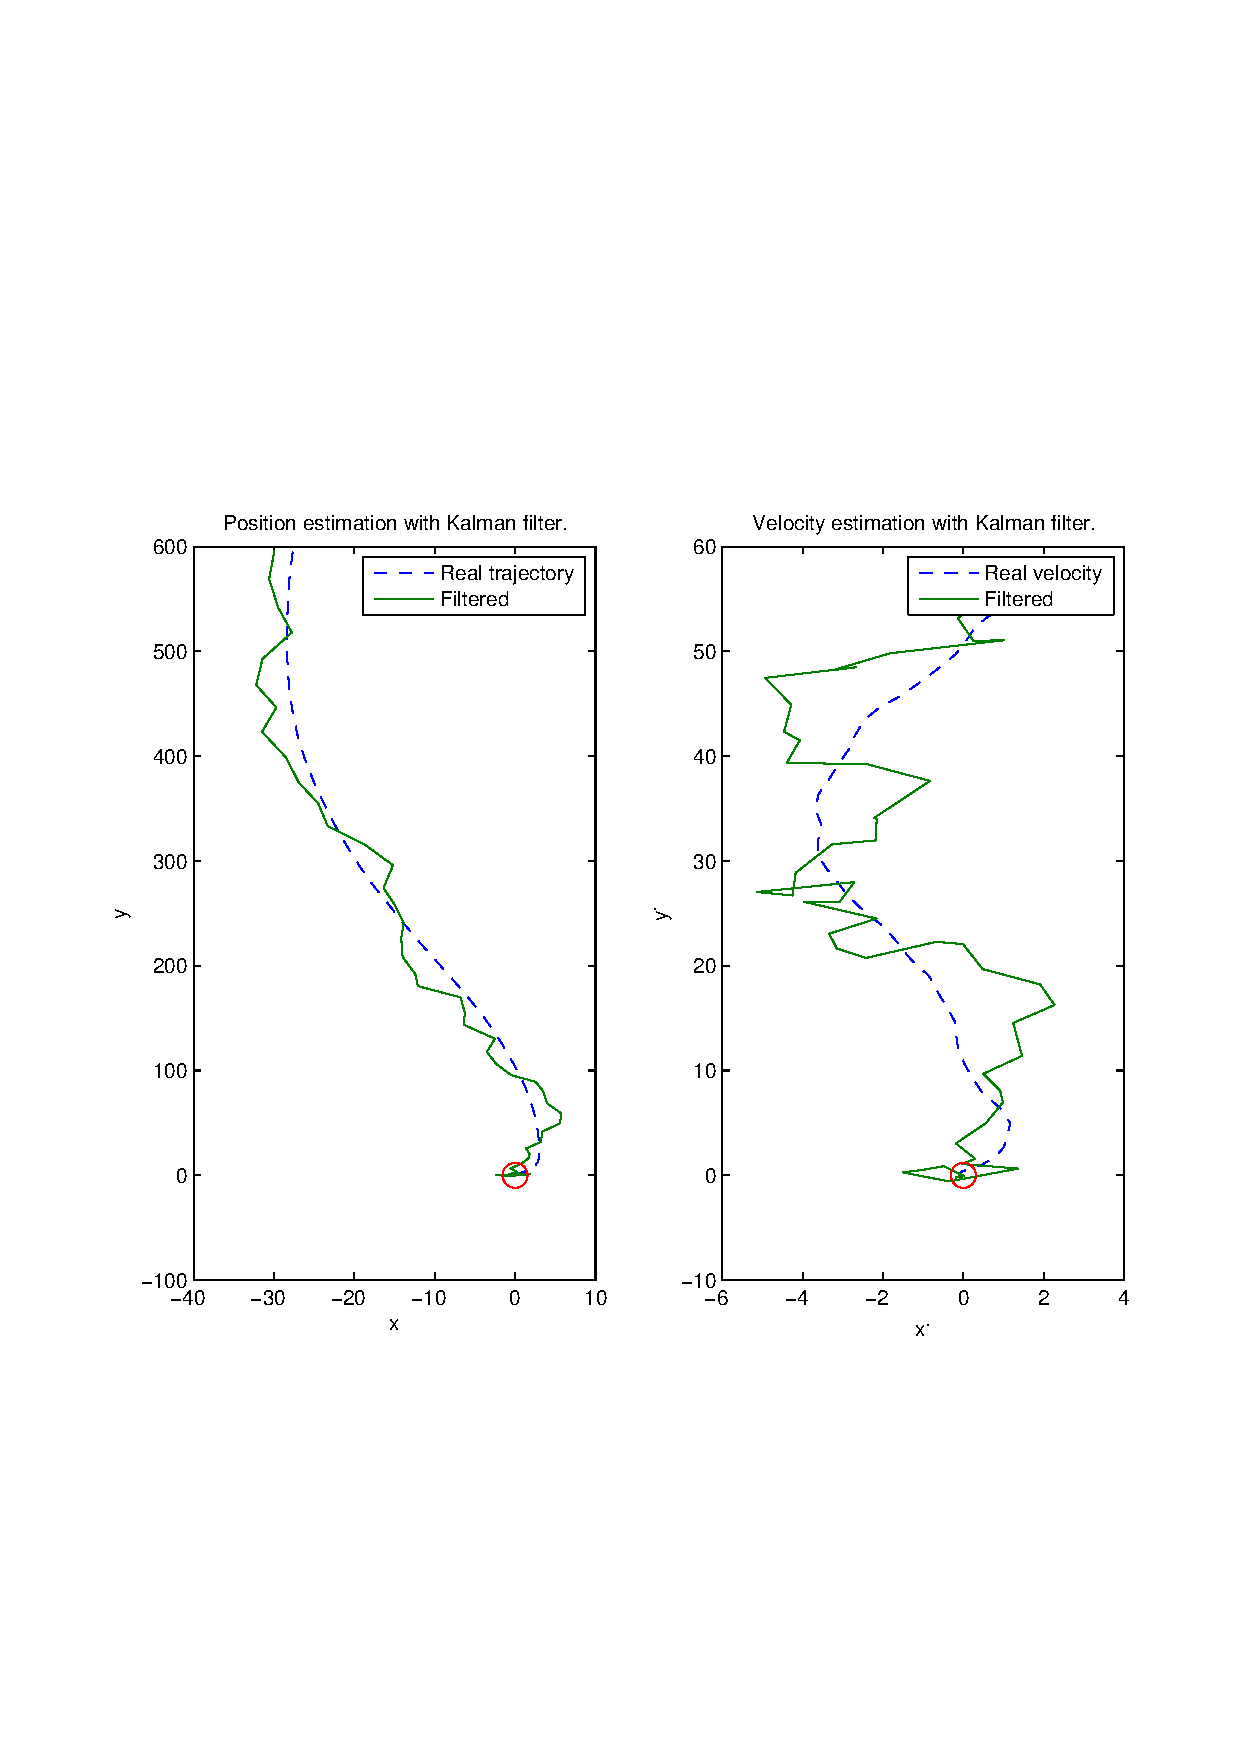
\includegraphics[width=5.5cm]{pics/demo1_f2}}
 \hspace{0.2cm}
 \subfigure[Smoother]{\label{fig:example1_3}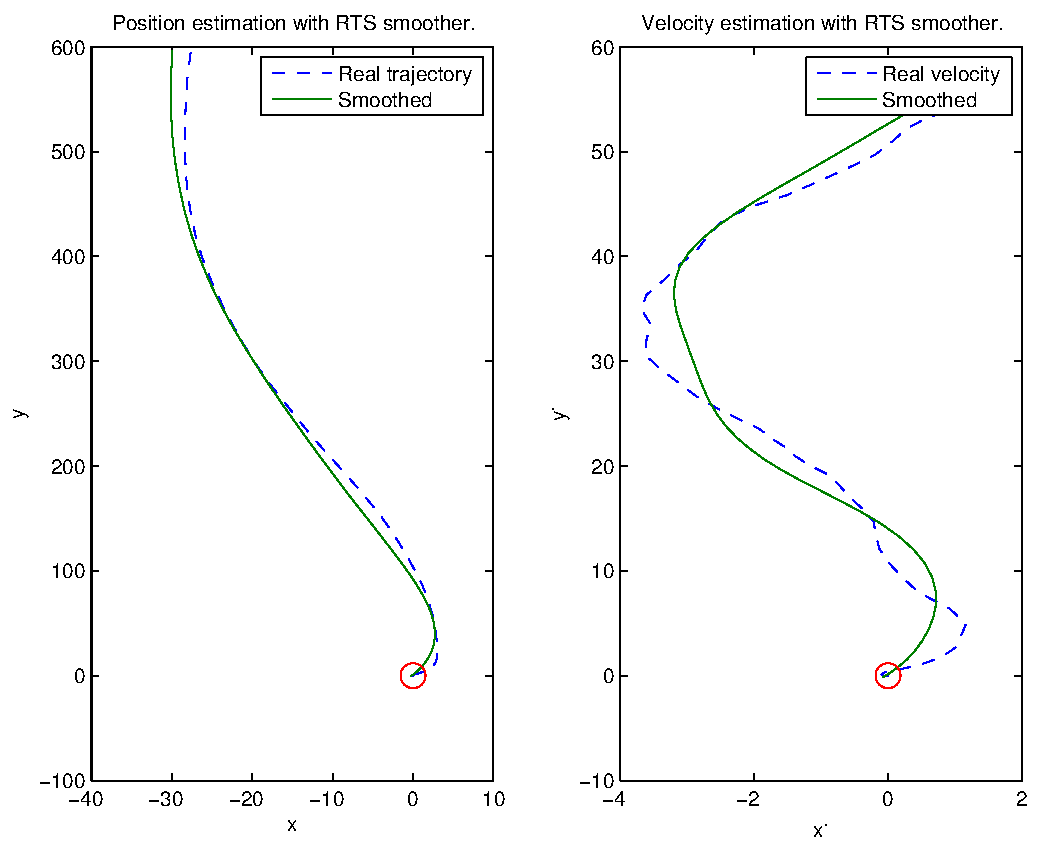
\includegraphics[width=5.5cm]{pics/demo1_f3}}
 %
 \caption{(a) Estimates for position and velocity of the moving object
  using the Kalman filter and CWPA model, and (b) Estimate for position and velocity of the moving object using the RTS smoother and CWPA model.}
 \label{fig:example1_2-3}
\end{figure}










%
%%%%%%%%%%%%%%%%%%%%%%%%%%%%%%%%%%%%%%%%%%%%%%%%%%%%%%%%%%%%%%%%%%%%%%%%%%%%%%

\clearpage
\newpage




%%%%%%%%%%%%%%%%%%%%%%%%%%%%%%%%%%%%%%%%%%%%%%%%%%%%%%%%%%%%%%%%%%%%%%%%%%%%%%
%
  %%%%%%%%%%%%%%%%%%%%%%%%%%%%%%%%%%%%%%%%%%%%%%%%%%%%%%%%%%%%%%%%%%%%%%%%%%%%%%
%
\chapter{Nonlinear State Space Estimation}
\label{ch:nonlinear-estimation}
%
%%%%%%%%%%%%%%%%%%%%%%%%%%%%%%%%%%%%%%%%%%%%%%%%%%%%%%%%%%%%%%%%%%%%%%%%%%%%%%

In many cases interesting dynamic systems are not linear by nature, so
the traditional Kalman filter cannot be applied in estimating the
state of such a system. In these kind of systems, both the dynamics
and the measurement processes can be nonlinear, or only one them. In
this section, we describe two extensions to the traditional Kalman
filter, which can be applied for estimating nonlinear dynamical
systems by forming Gaussian approximations to the joint distribution
of the state $\vec{x}$ and measurement $\vec{y}$. First we present the
Extended Kalman filter (EKF), which is based on Taylor series
approximation of the joint distribution, and then the Unscented Kalman
filter (UKF), which is respectively based on the unscented
transformation of the joint distribution. After UKF we review
Gauss-Hermite Kalman filter (GHKF) and third-order symmetric Cubature
Kalman filter (CKF).


%%%%%%%%%%%%%%%%%%%%%%%%%%%%%%%%%%%%%%%%%%%%%%%%%%%%%%%%%%%%%%%%%%%%%%%%%%%%%%
%


\section{Extended Kalman Filter}


\subsection{Taylor Series Based Approximations}

Next we present linear and quadratic approximations for the
distribution of variable $\vec{y}$, which is generated with a non-linear transformation
of a Gaussian random variable $\vec{x}$ as follows:
%
\begin{equation}
\begin{split}
  \vec{x} &\sim \N(\vec{m},\mat{P}) \\
  \vec{y} &= \vec{g}(\vec{x}),
\end{split}
\label{eq:trans_g}
\end{equation}
%
where $\vec{x} \in \spc{R}^n$, $\vec{y} \in \spc{R}^m$, and $\vec{g} :
\spc{R}^n \mapsto \spc{R}^m$ is a general non-linear function. Solving
the distribution of $\vec{y}$ formally is in general not possible,
because it is non-Gaussian for all by linear $\vec{g}$, so in practice
it must be approximated somehow. The joint distribution of $\vec{x}$
and $\vec{y}$ can be formed with, for example, linear and quadratic
approximations, which we present next. See, for example, \citet{Bar-Shalom+Li+Kirubarajan:2001} for the derivation of these approximations.

\subsection{Linear Approximation}

The linear approximation based Gaussian approximation of the joint
distribution of variables $\vec{x}$ and $\vec{y}$ defined by equations
(\ref{eq:trans_g}) is given as
  %
  \begin{equation}
     \begin{pmatrix}
       \vec{x} \\ \vec{y}
     \end{pmatrix} \sim
     \N\left(
     \begin{pmatrix}
       \vec{m} \\ \vecmu_L
     \end{pmatrix},
     \begin{pmatrix}
       \vec{P}   & \vec{C}_L \\
       \vec{C}_L^T & \mat{S}_L
     \end{pmatrix} \right),
  \end{equation}
  %
  where
  %
  \begin{equation}
  \begin{split}
  \vecmu_L &= \vec{g}(\vec{m}) \\
    \mat{S}_L &= \mat{G}_{\vec{x}}(\vec{m}) \, \mat{P} \,
    \mat{G}^T_{\vec{x}}(\vec{m}) \\
    \mat{C}_L &= \mat{P} \, \mat{G}^T_{\vec{x}}(\vec{m}),
  \end{split}
  \end{equation}
  %
  and $\mat{G}_{\vec{x}}(\vec{m})$ is the Jacobian matrix of $\vec{g}$
  with elements
  %
  \begin{equation}
    \left[ \mat{G}_{\vec{x}}(\vec{m}) \right]_{j,j'} =
    \frac{\partial g_j(\vec{x})}{\partial x_{j'}}
    \Bigg|_{\vec{x} = \vec{m}}.
  \label{eq:G1}
  \end{equation}

\subsection{Quadratic Approximation}

The quadratic approximations retain also the second order terms of the
Taylor series expansion of the non-linear function:
  %
  \begin{equation}
     \begin{pmatrix}
       \vec{x} \\ \vec{y}
     \end{pmatrix} \sim
     \N\left(
     \begin{pmatrix}
       \vec{m} \\ \vecmu_Q
     \end{pmatrix},
     \begin{pmatrix}
       \vec{P}   & \vec{C}_Q \\
       \vec{C}_Q^T & \mat{S}_Q
     \end{pmatrix} \right),
  \end{equation}
  %
  where the parameters are
  %
  \begin{equation}
  \begin{split}
  \vecmu_Q &= \vec{g}(\vec{m}) 
  + \frac{1}{2} \sum_i \vec{e}_i \, \tr\left\{
     \mat{G}_{\vec{x}\vec{x}}^{(i)}(\vec{m}) \,
    \mat{P} \right\} \\
    \mat{S}_Q &= \mat{G}_{\vec{x}}(\vec{m}) \, \mat{P} \, \mat{G}^T_{\vec{x}}(\vec{m})
  + \frac{1}{2} \sum_{i,i'} \vec{e}_i \, \vec{e}^T_{i'} \,
    \tr\left\{ \mat{G}_{\vec{x}\vec{x}}^{(i)}(\vec{m}) \, \mat{P} \,
     \mat{G}_{\vec{x}\vec{x}}^{(i')}(\vec{m}) \, \mat{P} \right\} \\
    \mat{C}_Q &= \mat{P} \, \mat{G}^T_{\vec{x}}(\vec{m}),
  \end{split}
  \end{equation}
%
  $\mat{G}_{\vec{x}}(\vec{m})$ is the Jacobian matrix \eqref{eq:G1}
  and $\mat{G}_{\vec{x}\vec{x}}^{(i)}(\vec{m})$ is the Hessian matrix
  of $g_i(\cdot)$ evaluated at $\vec{m}$:
%
\begin{equation}
   \left[ \mat{G}_{\vec{x}\vec{x}}^{(i)}(\vec{m}) \right]_{j,j'}
   = \frac{\partial^2 g_i(\vec{x})}{\partial x_j \, \partial x_{j'}},
  \Bigg|_{\vec{x} = \vec{m}}.
\end{equation}
%
$\vec{e}_i = (0~\cdots~0~1~0~\cdots~0)^T$ is the unit
vector in direction of the coordinate axis $i$.



\subsection{Extended Kalman filter}
%
%%%%%%%%%%%%%%%%%%%%%%%%%%%%%%%%%%%%%%%%%%%%%%%%%%%%%%%%%%%%%%%%%%%%%%%%%%%%%%

The extended Kalman filter \citep[see, for instance, ][]{Jazwinski:1966,
Maybeck:1982,Bar-Shalom+Li+Kirubarajan:2001,Grewal+Andrews:2001,Sarkka:2006} extends the scope of Kalman filter to nonlinear optimal
filtering problems by forming a Gaussian approximation to the joint
distribution of state $\vec{x}$ and measurements $\vec{y}$ using a
Taylor series based transformation. First and second order extended
Kalman filters are presented, which are based on linear and quadratic
approximations to the transformation. Higher order filters are also
possible, but not presented here.


The filtering model used in the EKF is
%
\begin{equation}
\begin{split}
\vec{x}_{k} &= \vec{f}(\vec{x}_{k-1},k-1) + \vec{q}_{k-1} \\
\vec{y}_{k} &= \vec{h}(\vec{x}_{k},k) + \vec{r}_{k},
\end{split} \label {eq:nonlinear_prob}
\end{equation}
%
where $\vec{x}_k \in \spc{R}^n$ is the state, $\vec{y}_k \in
\spc{R}^m$ is the measurement, $\vec{q}_{k-1} \sim
\N(\vec{0},\mat{Q}_{k-1})$ is the process noise, $\vec{r}_{k} \sim
\N(\vec{0},\mat{R}_{k})$ is the measurement noise, $\vec{f}$ is the
(possibly nonlinear) dynamic model function and $\vec{h}$ is the
(again possibly nonlinear) measurement model function. The first and
second order extended Kalman filters approximate the distribution of
state $\vec{x}_k$ given the observations $\vec{y}_{1:k}$ with a
Gaussian:
%
\begin{equation}
  p(\vec{x}_{k}\,|\,\vec{y}_{1:k}) \approx
    \N(\vec{x}_{k}\,|\,\vec{m}_{k},\mat{P}_{k}).
\end{equation}
%

\subsubsection{First Order Extended Kalman Filter}

Like Kalman filter, also the extended Kalman filter is separated to
two steps.  The steps for the first order EKF are as follows:
  %
  \begin{itemize}
  \item {\em Prediction:}
  %
  \begin{equation}
  \begin{split}
    \vec{m}^-_{k} &= \vec{f}(\vec{m}_{k-1},k-1) \\
    \mat{P}^-_{k} &= \mat{F}_{\vec{x}}(\vec{m}_{k-1},k-1) \, \mat{P}_{k-1} \,
     \mat{F}_{\vec{x}}^T (\vec{m}_{k-1},k-1) + \mat{Q}_{k-1}.
  \end{split}
  \label{eq:dekf_predict1}
  \end{equation}
  
  \item {\em Update:}
  %
  \begin{equation}
  \begin{split}
    \vec{v}_{k} &= \vec{y}_k - \mat{h} (\vec{m}^-_{k},k) \\
    \vec{S}_{k} &= \mat{H}_{\vec{x}}(\vec{m}^-_{k},k) \, \mat{P}^-_{k} \,
    \mat{H}^T_{\vec{x}}(\vec{m}^-_{k},k) + \vec{R}_{k} \\
    \vec{K}_{k} &= \mat{P}^-_{k} \, \mat{H}^T_{\vec{x}}(\vec{m}^-_{k},k) \,
    \vec{S}^{-1}_{k} \\
    \vec{m}_{k} &= \vec{m}^-_{k} + \vec{K}_{k} \, \vec{v}_k \\
    \mat{P}_{k} &= \mat{P}^-_{k} - \vec{K}_{k} \, \vec{S}_{k} \, \vec{K}^T_{k},
  \end{split}
  \label{eq:dekf_update1}
  \end{equation}
  \end{itemize}
  %
  where the matrices $\mat{F}_{\vec{x}}(\vec{m},k-1)$ and
  $\mat{H}_{\vec{x}}(\vec{m},k)$ are the Jacobians of
  $\vec{f}$ and $\vec{h}$, with elements
  %
  \begin{align}
    \left[ \mat{F}_{\vec{x}}(\vec{m},k-1) \right]_{j,j'} =
    \frac{\partial f_j(\vec{x},k-1)}{\partial x_{j'}}
    \Bigg|_{\vec{x} = \vec{m}}
  \label{eq:F1} \\
    \left[ \mat{H}_{\vec{x}}(\vec{m},k) \right]_{j,j'} =
    \frac{\partial h_j(\vec{x},k)}{\partial x_{j'}}
    \Bigg|_{\vec{x} = \vec{m}}.
  \label{eq:H1}
  \end{align}
%
Note that the difference between first order EKF and KF is that the
matrices $\mat{A}_k$ and $\mat{H}_k$ in KF are replaced with Jacobian
matrices $\mat{F}_{\vec{x}}(\vec{m}_{k-1},k-1)$ and
$\mat{H}_{\vec{x}}(\vec{m}_k^-,k)$ in EKF. Predicted mean
$\vec{m}_k^-$ and residual of prediction $\vec{v}_k$ are also
calculated differently in the EKF.  In this toolbox the prediction and
update steps of the first order EKF can be computed with functions
\texttt{ekf\_predict1} and \texttt{ekf\_update1}, respectively.

\subsubsection{Second Order Extended Kalman Filter}

The corresponding steps for the second order EKF are as follows:
  %
  \begin{itemize}
  \item {\em Prediction:}
  %
  \begin{equation}
  \begin{split}
    \vec{m}^-_{k} &= \vec{f}(\vec{m}_{k-1},k-1) 
    + \frac{1}{2} \sum_i \vec{e}_i \,
      \tr\left\{ \mat{F}_{\vec{x}\vec{x}}^{(i)}(\vec{m}_{k-1},k-1) \,
      \mat{P}_{k-1} \right\} \\
    \mat{P}^-_{k} &= \mat{F}_{\vec{x}}(\vec{m}_{k-1},k-1) \, \mat{P}_{k-1} \,
     \mat{F}^T_{\vec{x}}(\vec{m}_{k-1},k-1) \\
   &+ \frac{1}{2} \sum_{i,i'} \vec{e}_i \, \vec{e}^T_{i'}
      \tr\left\{ \mat{F}_{\vec{x}\vec{x}}^{(i)}(\vec{m}_{k-1},k-1) \mat{P}_{k-1} 
       \mat{F}_{\vec{x}\vec{x}}^{(i')}(\vec{m}_{k-1},k-1) \mat{P}_{k-1} \right\} \\
    &+ \mat{Q}_{k-1}.
  \end{split}
  \label{eq:dekf_predict2}
  \end{equation}

  \item {\em Update:}
  %
  \begin{equation}
  \begin{split}
    \vec{v}_{k} &= \vec{y}_k - \mat{h} (\vec{m}^-_{k},k) 
    - \frac{1}{2} \sum_i \vec{e}_i \,
      \tr\left\{ \mat{H}_{\vec{x}\vec{x}}^{(i)}(\vec{m}^-_{k},k) \,
      \mat{P}^-_{k} \right\} \\
    \vec{S}_{k} &= \mat{H}_{\vec{x}}(\vec{m}^-_{k},k) \, \mat{P}^-_{k} \,
    \mat{H}^T_{\vec{x}}(\vec{m}^-_{k},k) \\
    &\quad + \frac{1}{2} \sum_{i,i'} \vec{e}_i \, \vec{e}^T_{i'} \,
      \tr\left\{ \mat{H}_{\vec{x}\vec{x}}^{(i)}(\vec{m}^-_{k},k) \, \mat{P}^-_{k} \,
       \mat{H}_{\vec{x}\vec{x}}^{(i')}(\vec{m}^-_{k},k) \, \mat{P}^-_{k} \right\} 
    + \vec{R}_{k} \\
    \vec{K}_{k} &= \mat{P}^-_{k} \,
    \mat{H}^T_{\vec{x}}(\vec{m}^-_{k},k) \, \vec{S}^{-1}_{k} \\
    \vec{m}_{k} &= \vec{m}^-_{k} + \vec{K}_{k} \, \vec{v}_k \\
    \mat{P}_{k} &= \mat{P}^-_{k} - \vec{K}_{k} \, \vec{S}_{k} \, \vec{K}^T_{k},
  \end{split}
  \label{eq:dekf_update2}
  \end{equation}
  \end{itemize}
  %
  where matrices $\mat{F}_{\vec{x}}(\vec{m},k-1)$ and
  $\mat{H}_{\vec{x}}(\vec{m},k)$ are Jacobians as in the first order EKF, given by
  Equations \eqref{eq:F1} and \eqref{eq:H1}. The matrices
  $\mat{F}^{(i)}_{\vec{x}\vec{x}}(\vec{m},k-1)$ and
  $\mat{H}^{(i)}_{\vec{x}\vec{x}}(\vec{m},k)$ are the Hessian matrices
  of $f_i$ and $h_i$:
  \begin{align}
   \left[ \mat{F}_{\vec{x}\vec{x}}^{(i)}(\vec{m},k-1) \right]_{j,j'}
   = \frac{\partial^2 f_i(\vec{x},k-1)}{\partial x_j \, \partial x_{j'}}
  \Bigg|_{\vec{x} = \vec{m}}
  \label{eq:F2} \\
   \left[ \mat{H}_{\vec{x}\vec{x}}^{(i)}(\vec{m},k) \right]_{j,j'}
   = \frac{\partial^2 h_i(\vec{x},k)}{\partial x_j \, \partial x_{j'}}
  \Bigg|_{\vec{x} = \vec{m}},
  \label{eq:H2}
  \end{align}
%
$\vec{e}_i = (0~\cdots~0~1~0~\cdots~0)^T$ is a unit vector in direction of the
coordinate axis $i$, that is, it has a $1$ at position $i$ and $0$ at other positions.

The prediction and update steps of the second order EKF can be
computed in this toolbox with functions \texttt{ekf\_predict2} and
\texttt{ekf\_update2}, respectively. By taking the second order terms
into account, however, doesn't quarantee, that the results get any
better. Depending on problem they might even get worse, as we shall
see in the later examples.

\subsection{The Limitations of EKF}

As discussed in, for example, \citep{Julier+Uhlmann:2004} the EKF has a
few serious drawbacks, which should be kept in mind when it's used:
%
\begin{enumerate}
\item As we shall see in some of the later demonstrations, the linear
  and quadratic transformations produces realiable results only when
  the error propagation can be well approximated by a linear or a
  quadratic function. If this condition is not met, the performance of
  the filter can be extremely poor. At worst, its estimates can
  diverge altogether.
\item The Jacobian matrices (and Hessian matrices with second order
  filters) need to exist so that the transformation can be applied.
  However, there are cases, where this isn't true. For example, the
  system might be jump-linear, in which the parameters can change
  abruptly \citep{Julier+Uhlmann:2004}.
\item In many cases the calculation of Jacobian and Hessian matrices
  can be a very difficult process, and its also prone to human errors
  (both derivation and programming). These errors are usually very
  hard to debug, as its hard to see which parts of the system produces
  the errors by looking at the estimates, especially as usually we
  don't know which kind of performance we should expect. For example,
  in the last demonstration (Reentry Vehicle Tracking) the first order
  derivatives were quite troublesome to calcute, even though the
  equations themselves were relatively simple. The second order
  derivatives would have even taken many more times of work.
\end{enumerate}
%
\label{page:ekf_problems}


  

%%%%%%%%%%%%%%%%%%%%%%%%%%%%%%%%%%%%%%%%%%%%%%%%%%%%%%%%%%%%%%%%%%%%%%%%%%%%%%
%
\subsection{Extended Kalman smoother}
%
%%%%%%%%%%%%%%%%%%%%%%%%%%%%%%%%%%%%%%%%%%%%%%%%%%%%%%%%%%%%%%%%%%%%%%%%%%%%%%

The difference between the first order extended Kalman smoother \citep{Cox:1964,Sage+Melsa:1971} and the traditional Kalman smoother is the
same as the difference between first order EKF and KF, that is, matrix
$\mat{A}_k$ in Kalman smoother is replaced with Jacobian
$\mat{F}_{\vec{x}}(\vec{m}_{k-1},k-1)$, and $\vec{m}_{k+1}^-$ is
calculated using the model function $\vec{f}$.  Thus, the equations
for the extended Kalman smoother can be written as
%
\begin{equation}
\begin{split}
    \vec{m}^-_{k+1} &= \vec{f}(\vec{m}_{k},k) \\
    \mat{P}^-_{k+1} &= \mat{F}_{\vec{x}}(\vec{m}_{k},k) \, \mat{P}_{k} \,
     \mat{F}_{\vec{x}}^T(\vec{m}_{k},k) + \mat{Q}_{k} \\
    \vec{C}_{k} &= \mat{P}_k \, \mat{F}_{\vec{x}}^T(\vec{m}_{k},k) \,
      [\mat{P}^-_{k+1}]^{-1} \\
    \vec{m}^s_k &= \vec{m}_k
    + \mat{C}_k \, [\vec{m}^s_{k+1} - \vec{m}^-_{k+1}] \\
    \mat{P}^s_k &= \mat{P}_k
    + \mat{C}_k \, [\mat{P}^s_{k+1} - \mat{P}^-_{k+1}] \, \mat{C}^T_k.
    \label{eq:derts}
\end{split}
\end{equation}
%
First order smoothing solutiong with a RTS type smoother can be
computed with function \texttt{erts\_smooth1}, and with
forward-backward type smoother the computation can be done with
function \texttt{etf\_smooth1}.

Higher order smoothers are also possible, but not described here, as
they are not currently implemented in this toolbox.

%%%%%%%%%%%%%%%%%%%%%%%%%%%%%%%%%%%%%%%%%%%%%%%%%%%%%%%%%%%%%%%%%%%%%%%%%%%%%%
%
\section{Demonstration: Tracking a random sine signal}
%
%%%%%%%%%%%%%%%%%%%%%%%%%%%%%%%%%%%%%%%%%%%%%%%%%%%%%%%%%%%%%%%%%%%%%%%%%%%%%%
Next we consider a simple, yet practical, example of a nonlinear
dynamic system, in which we estimate a random sine signal using the
extended Kalman filter. By random we mean that the angular velocity
and the amplitude of the signal can vary through time. In this example
the nonlinearity in the system is expressed through the measurement
model, but it would also be possible to express it with the dynamic
model and let the measurement model be linear.

The state vector in this case can be expressed as
%
\begin{equation}
%
\vec{x}_k = 
\begin{pmatrix}
\theta_k & \omega_k & a_k
\end{pmatrix}^T,
%
\end{equation}
%
where $\theta_k$ is the parameter for the sine function on time step
$k$, $\omega_k$ is the angular velocity on time step $k$ and $a_k$ is
the amplitude on time step $k$. The evolution of parameter $\theta$ is
modelled with a discretized Wiener velocity model, where the velocity
is now the angular velocity:
%
\begin{equation}
%
\frac{d \theta}{d t} = \omega.
%
\end{equation}
%
The values of $\omega$ and $a$ are perturbed with one dimensional
white noise processes $w_a(t)$ and $w_w(t)$, so the signal isn't
totally deterministic:
%
\begin{eqnarray}
%
\frac{da}{dt} &=& w_a(t) \\ \frac{dw}{dt} &=& w_w(t).
%
\end{eqnarray}
%
Thus, the continous-time dynamic equation can be written as
%
\begin{equation}
%
\frac{d \vec{x}(t)}{dt} = \begin{pmatrix} 0 & 1 & 0\\ 0 & 0 & 0\\ 0 &
0 & 0
\end{pmatrix}\vec{x}(t) +
\begin{pmatrix} 0 & 0 \\ 1 & 0 \\ 0 & 1
\end{pmatrix}\vec{w}(t), \label{eq:sine_cont_model}
%
\end{equation}
%
where the white noise process $\vec{w}(t)$ has power spectral density
%
\begin{equation}
%
\mat{Q}_c = \begin{pmatrix} q_1 & 0 \\ 0 & q_2
\end{pmatrix}.
%
\end{equation}
%
Variables $q_1$ and $q_2$ describe the strengths of random
perturbations of the angular velocity and the amplitude, respectively,
which are in this demonstration are set to $q_1 = 0.2$ and $q_2 =
0.1$. By using the equation (\ref{eq:ode_ak}) the discretized form of
the dynamic equation can written as
%
\begin{equation}
%
\vec{x}_k = \begin{pmatrix} 1 & \dt & 0\\ 0 & 1 & 0\\ 0 & 0 & 1
\end{pmatrix}\vec{x}_{k-1} + \vec{q}_{k-1},
%
\end{equation}
%
where $\dt$ is the step size (with value $\dt = 0.01$ in this case),
and using the equation (\ref{eq:ode_qk}) the covariance matrix
$\mat{Q}_{k-1}$ of the discrete Gaussian white noise process
$\vec{q}_{k-1} \sim N(\vec{0},\mat{Q}_{k-1})$ can be easily computed
to give
%
\begin{equation}
%
\mat{Q}_{k-1} = \begin{pmatrix} \frac{1}{3}\dt^3q_1 &
\frac{1}{2}\dt^2q_1 & 0\\ \frac{1}{2}\dt^2q_1 & \dt q_1 & 0\\ 0 & 0 &
\dt q_2
\end{pmatrix}.
\end{equation}
%

As stated above, the non-linearity in this case is expressed by the
measurement model, that is, we propagate the current state through a
non-linear measurement function $\vec{h}(\vec{x}_{k},k)$ to get an
actual measurement. Naturally the function in this case is the actual
sine function
%
\begin{equation}
%
\vec{h}(\vec{x}_{k},k) = a_k\sin(\theta_k). \label{eq:ekf_demo1_h}
%
\end{equation}
%
With this the measurement model can be written as
%
\begin{equation}
%
y_k = \vec{h}(\vec{x}_k,k) + r_k = a_k\sin(\theta_k) + r_k,
%
\end{equation}
%
where $r_k$ is white, univariate Gaussian noise with zero mean and
variance $\sigma_r = 1$.
 
The derivatives of the measurement function with respect to state
variables are
%
\begin{equation}
\begin{split}
%
\frac{\partial \vec{h}(\vec{x}_{k},k)}{\partial \theta_k} &=
a_k\cos(\theta_k)\\ \frac{\partial \vec{h}(\vec{x}_{k},k)}{\partial
\omega_k} &= 0\\ \frac{\partial \vec{h}(\vec{x}_{k},k)}{\partial a_k}
&= \sin(\theta_k),
%
\end{split}
\end{equation}
%
so the Jacobian matrix (actually in this case, a vector, as the
measurements are only one dimensional) needed by the EKF can be
written as
%
\begin{equation}
%
\mat{H}_{\vec{x}}(\vec{m},k) = \begin{pmatrix} a_k\cos(\theta_k) & 0 &
\sin(\theta_k) \label{eq:ekf_demo1_jacobian}
\end{pmatrix}.
%
\end{equation}
%

We also filter the signal with second order EKF, so we need to
evaluate the Hessian matrix of the measurement model function.  In
this case the second order derivatives of $\vec{h}$ with respect to
all state variables can written as

\begin{equation}
\begin{split}
%
\frac{\partial^2 \vec{h}(\vec{x}_{k},k)}{\partial \theta_k \partial
\theta_k} &= -a_k\sin(\theta_k)\\ \frac{\partial^2
\vec{h}(\vec{x}_{k},k)}{\partial \theta_k \partial \omega_k} &= 0\\
\frac{\partial^2 \vec{h}(\vec{x}_{k},k)}{\partial \theta_k \partial
a_k} &= \cos(\theta_k)\\ \frac{\partial^2
\vec{h}(\vec{x}_{k},k)}{\partial \omega_k \partial \omega_k} &= 0\\
\frac{\partial^2 \vec{h}(\vec{x}_{k},k)}{\partial \omega_k \partial
a_k} &= 0\\ \frac{\partial^2 \vec{h}(\vec{x}_{k},k)}{\partial a_k
\partial a_k} &= 0.
%
\end{split}
\end{equation} With these the Hessian matrix can expressed as
%
\begin{equation}
%
\mat{H}_{\vec{xx}}(\vec{m},k) = \begin{pmatrix} -a_k\sin(\theta_k) & 0
& \cos(\theta_k) \\ 0 & 0 & 0 \\ \cos(\theta_k) & 0 & 0
\label{eq:ekf_demo1_hessian}
\end{pmatrix}.
%
\end{equation}
%
Note that as the measurements are only one dimensional we need to
evaluate only one Hessian, and as the expressions are rather simple
the computation of this Hessian is trivial. In case of higher
dimensions we would need to evaluate the Hessian for each dimension
separately, which could easily result in high amount of dense algebra.


In this demonstration program the measurement function
(\ref{eq:ekf_demo1_h}) is computed with the following code:
%
\begin{lstlisting} 
function Y = ekf_demo1_h(x,param) 
  f = x(1,:); 
  a = x(3,:); 
  Y = a.*sin(f); 
  if size(x,1) == 7 
     Y = Y + x(7,:); 
  end
\end{lstlisting}
%
where the parameter \texttt{x} is a vector containing a single state
value, or a matrix containing multiple state values. It is also
necessary to include the parameter \texttt{param}, which contains the
other possible parameters for the functions (not present in this
case). The last three lines are included for the augmented version of
unscented Kalman filter (UKF), which is described later in this
document.  The Jacobian matrix of the measurement function (eq.
(\ref{eq:ekf_demo1_jacobian})) is computed with the following
function:
%
\begin{lstlisting} 
function dY = ekf_demo1_dh_dx(x, param) 
  f = x(1,:); 
  w = x(2,:); 
  a = x(3,:); 
  dY = [(a.*cos(f))' zeros(size(f,2),1) (sin(f))'];
\end{lstlisting}
%
The Hessian matrix of the measurement function (eq.
\ref{eq:ekf_demo1_hessian}) is computed with the following function:
%
\begin{lstlisting} 
function df = ekf_sine_d2h_dx2(x,param) 
  f = x(1); 
  a = x(3);
  df = zeros(1,3,3); 
  df(1,:,:) = [-a*sin(f) 0 cos(f); 0 0 0; cos(f) 0 0];
\end{lstlisting}
% 
These functions are defined in files \texttt{efk\_sine\_h.m},
\texttt{ekf\_sine\_dh\_dx.m} and \texttt{ekf\_sine\_d2h\_dx2.m},
respectively. The handles of these functions are saved in the actual
demonstration script file (\texttt{ekf\_sine\_demo.m}) with the
following code lines:
%
\begin{lstlisting} 
h_func = @ekf_sine_h; 
dh_dx_func = @ekf_sine_dh_dx;
d2h_dx2_func = @ekf_sine_d2h_dx2;
\end{lstlisting}
%

It is also important to check out that the implementation on
calculating the derivatives is done right, as it is, especially with
more complex models, easy to make errors in the equations. This can be
done with function \texttt{der\_check}:
%
\begin{lstlisting} 
der_check(h_func, dh_dx_func, 1, [f w a]');
\end{lstlisting}
%
The third parameter with value \texttt{1} signals that we want to test
the derivative of function's first (and in this case the only)
dimension.  Above we have assumed, that the variable \texttt{f}
contains the parameter value for the sine function, \texttt{w} the
angular velocity of the signal and \texttt{a} the amplitude of the
signal.

After we have discretized the dynamic model and generated the real
states and measurements same as in the previous example (the actual
code lines are not stated here, see the full source code at end of
this document), we can use the EKF to get the filtered estimates for
the state means and covariances. The filtering (with first order EKF)
is done almost the same as in the previous example:
%
\begin{lstlisting} 
MM = zeros(size(M,1),size(Y,2)); PP =
zeros(size(M,1),size(M,1),size(Y,2));

for k=1:size(Y,2) 
  [M,P] = ekf_predict1(M,P,A,Q); 
  [M,P] = ekf_update1(M,P,Y(:,k),dh_dx_func,R*eye(1),h_func); 
  MM(:,k) = M;
  PP(:,:,k) = P; 
end
\end{lstlisting}
%
As the model dynamics are in this case linear the prediction step
functions exactly the same as in the case of traditional Kalman
filter. In update step we pass the handles to the measurement model
function and it's derivative function and the variance of measurement
noise (parameters 6, 4 and 5, respectively), in addition to other
parameters. These functions also have additional parameters, which
might be needed in some cases. For example, the dynamic and
measurement model functions might have parameters, which are needed
when those functions are called. See the full function specifications
in chapter~\ref{ch:functions} for more details about the parameters.

With second order EKF the filtering loop remains almost the same with
the exception of update step:
%
\begin{lstlisting} 
MM2 = zeros(size(M,1),size(Y,2)); 
PP2 = zeros(size(M,1),size(M,1),size(Y,2));

for k=1:size(Y,2) 
  [M,P] = ekf_predict1(M,P,A,Q); 
  [M,P] = ekf_update2(M,P,Y(:,k),dh_dx_func,...  
    d2h_dx2_func,R*eye(1),h_func);
  MM(:,k) = M; PP(:,:,k) = P; 
end
\end{lstlisting}
%


The smoothing of state estimates using the extended RTS smoother is
done sameways as in the previous example:
%
\begin{lstlisting} 
[SM1,SP1] = erts_smooth1(MM,PP,A,Q);
\end{lstlisting}
%
With the extended forward-backward smoother the smoothing is done with
the following function call:
%
\begin{lstlisting} 
[SM2,SP2] = etf_smooth1(MM,PP,Y,A,Q,[],[],[],...
  dh_dx_func,R*eye(1),h_func);
\end{lstlisting}
%
Here we have assigned empty vectors for parameters 6,7 and 8 (inverse
prediction, its derivative w.r.t. to noise and its parameters,
respectively), because they are not needed in this case.

To visualize the filtered and smoothed signal estimates we must
evaluate the measurement model function with every state estimate to
project the estimates to the measurement space. This can be done with
the built-in Matlab function \texttt{feval}:
%
\begin{lstlisting} 
Y_m = feval(h_func, MM);
\end{lstlisting}
%
The filtered and smoothed estimates of the signals using the first
order EKF, ERTS and ETF are plotted in figures \ref{fig:example2_1},
\ref{fig:example2_2} and \ref{fig:example2_3}, respectively. The
estimates produced by second order EKF are not plotted as they do not
differ much from first order ones.  As can be seen from the figures
both smoothers give clearly better estimates than the
filter. Especially in the beginning of the signal it takes a while for
the filter to catch on to right track.


\label{page:sine_rmse}

The difference between the smoothers doesn't become clear just by
looking these figures. In some cases the forward-backward smoother
gives a little better estimates, but it tends to be more sensitive
about numerical accuracy and the process and measurement noises. To
make a comparison between the performances of different methods we
have listed the average of root mean square errors (RMSE) on 100 Monte
Carlo simulations with different methods in table
\ref{table:sine_errors}.  In addition to RMSE of each state variable
we also provide the estimation error in measurement space, because we
might be more interested in estimating the actual value of signal than
its components.  Usually, however, the primary goal of these methods
is to estimate the hidden state variables. The following methods were
used:
%
\begin{itemize}
\item EKF1: First order extended Kalman filter.
\item ERTS1: First order extended Rauch-Tung-Striebel smoother.
\item ETF1: First order extended Forward-Backward smoother.
\item EKF2: Second order extended Kalman filter.
\item ERTS2: First order extended Rauch-Tung-Striebel smoother applied
to second order EKF estimates.
\item ETF2: First order extended Forward-Backward smoother applied to
second order EKF estimates.
\item UKF: unscented Kalman filter.
\item URTS: unscented Rauch-Tung-Striebel smoother.
\end{itemize}
%
From the errors we can see that with filters EKF2 gives clearly the
lowest errors with variables $\theta$ and $a$. Due to this also with
smoothers ERTS2 and ETF2 give clearly lower errors than others. On the
other hand EKF1 gives the lowest estimation error with variable
$\omega$. Furthermore, with filters EKF1 also gives lowest error in
measurement space. Each smoother, however, gives approximately the
same error in measurement space. It can also be seen, that the UKF
functions the worst in this case. This is due to linear and quadratic
approximations used in EKF working well with this model. However, with
more nonlinear models UKF is often superior over EKF, as we shall see
in later sections.

In all, none of the used methods proved to be clearly superior over
the others with this model. It is clear, however, that EKF should be
preferred over UKF as it gives lower error and is slightly less
demanding in terms of computation power.  Whether first or second
order EKF should be used is ultimately up to the goal of
application. If the actual signal value is of interest, which is
usually the case, then one should use first order EKF, but second
order one might better at predicting new signal values as the
variables $\theta$ and $a$ are closer to real ones on average.

\begin{figure}
\begin{center}
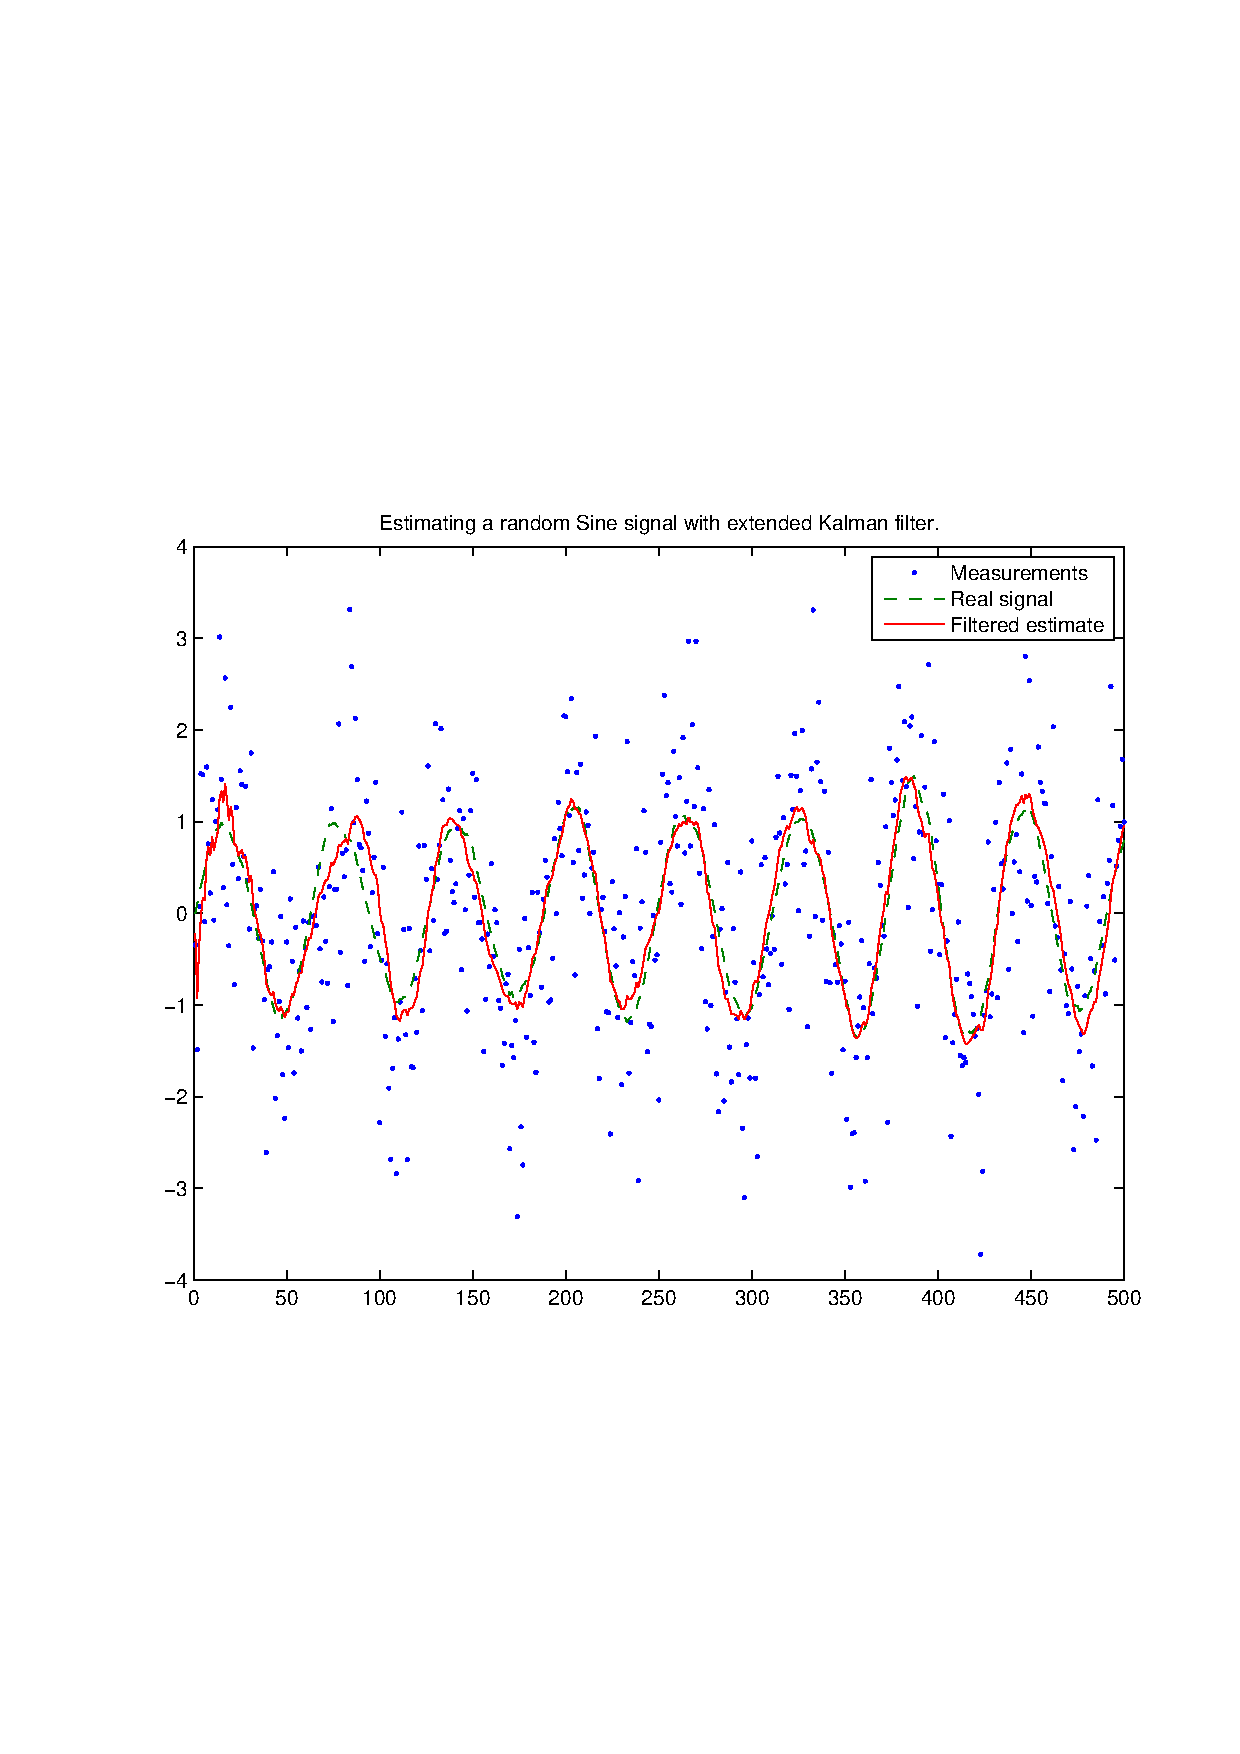
\includegraphics[width=11cm]{pics/demo2_f1}
\caption{Filtered estimate of the sine signal using the first order
extended Kalman filter.}
\label{fig:example2_1}
\end{center}
\end{figure}

\begin{figure}
\begin{center}
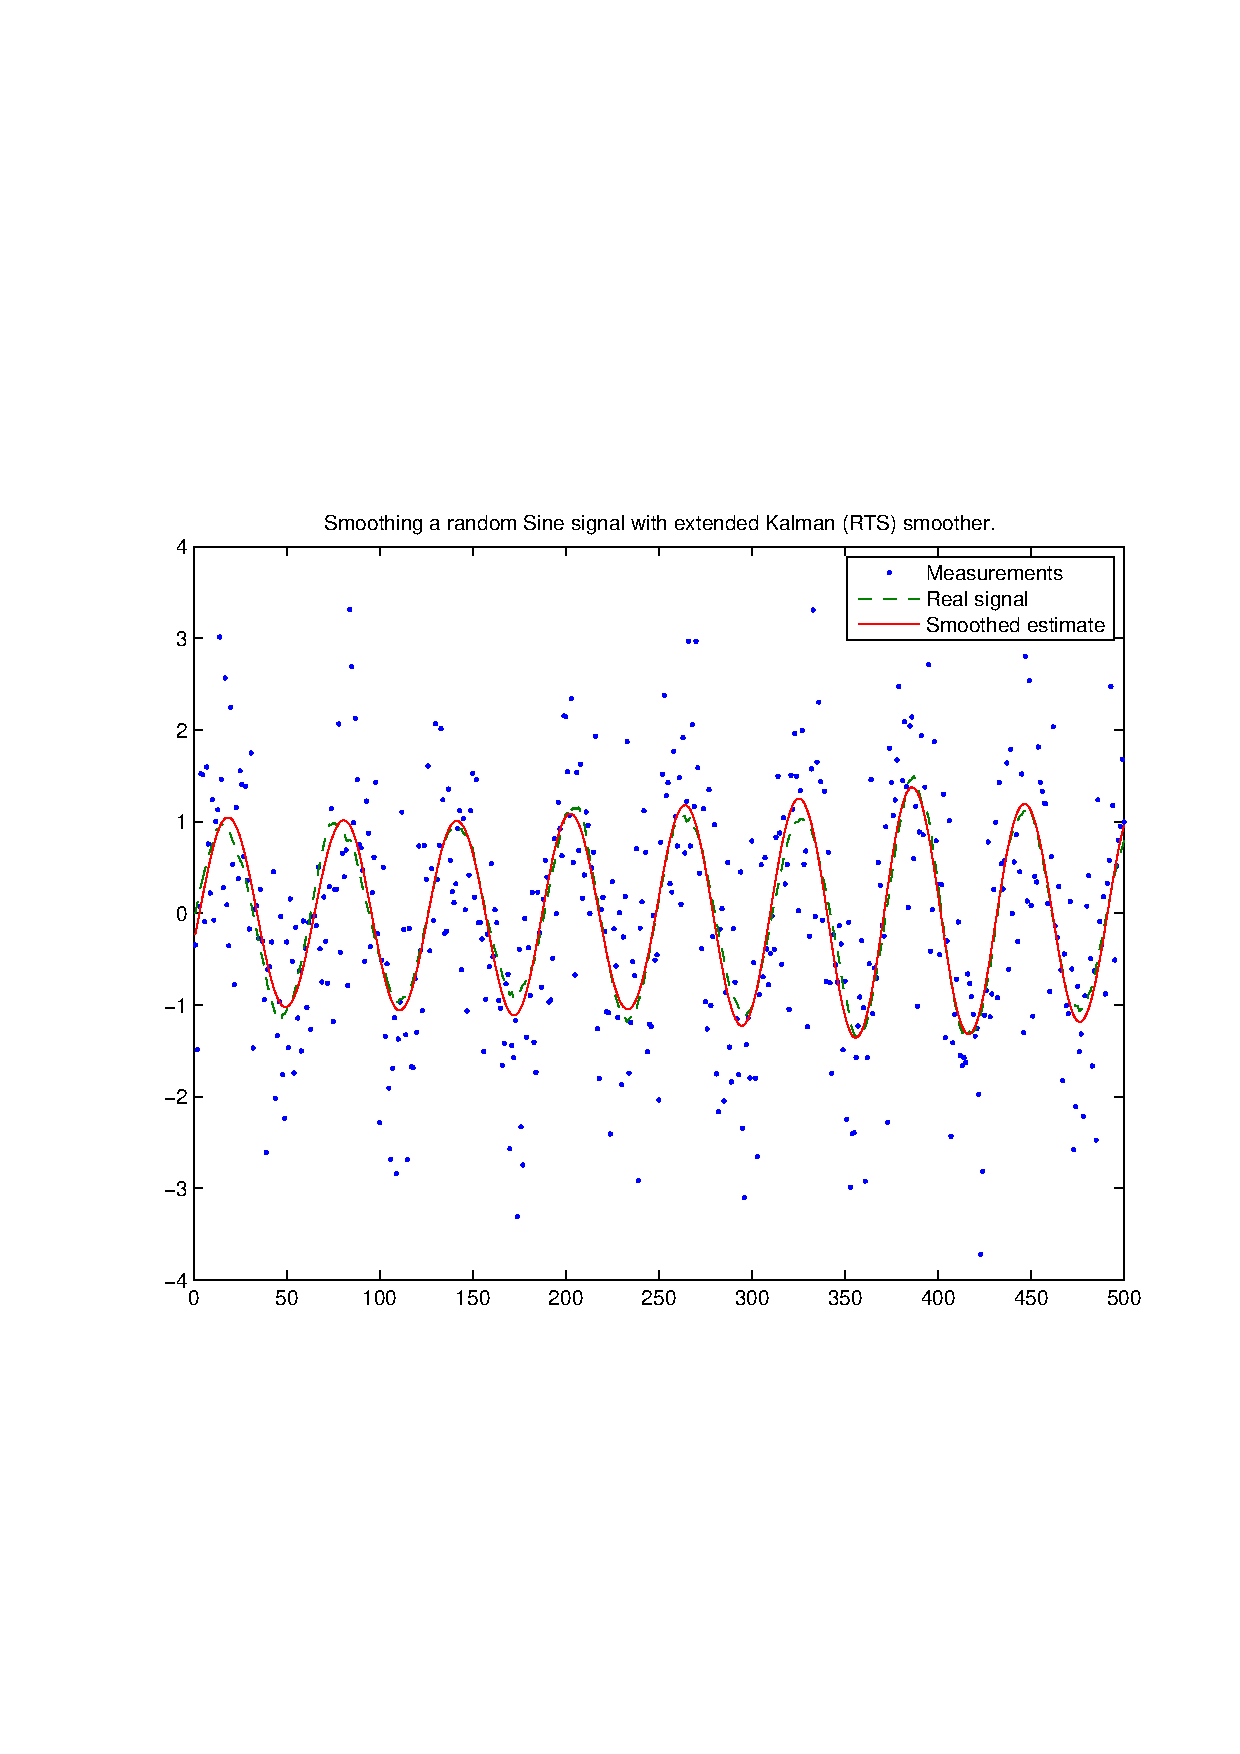
\includegraphics[width=11cm]{pics/demo2_f2}
\caption{Smoothed estimate of the sine signal using the extended
Kalman (RTS) smoother.}
\label{fig:example2_2}
\end{center}
\end{figure}

\begin{figure}
\begin{center}
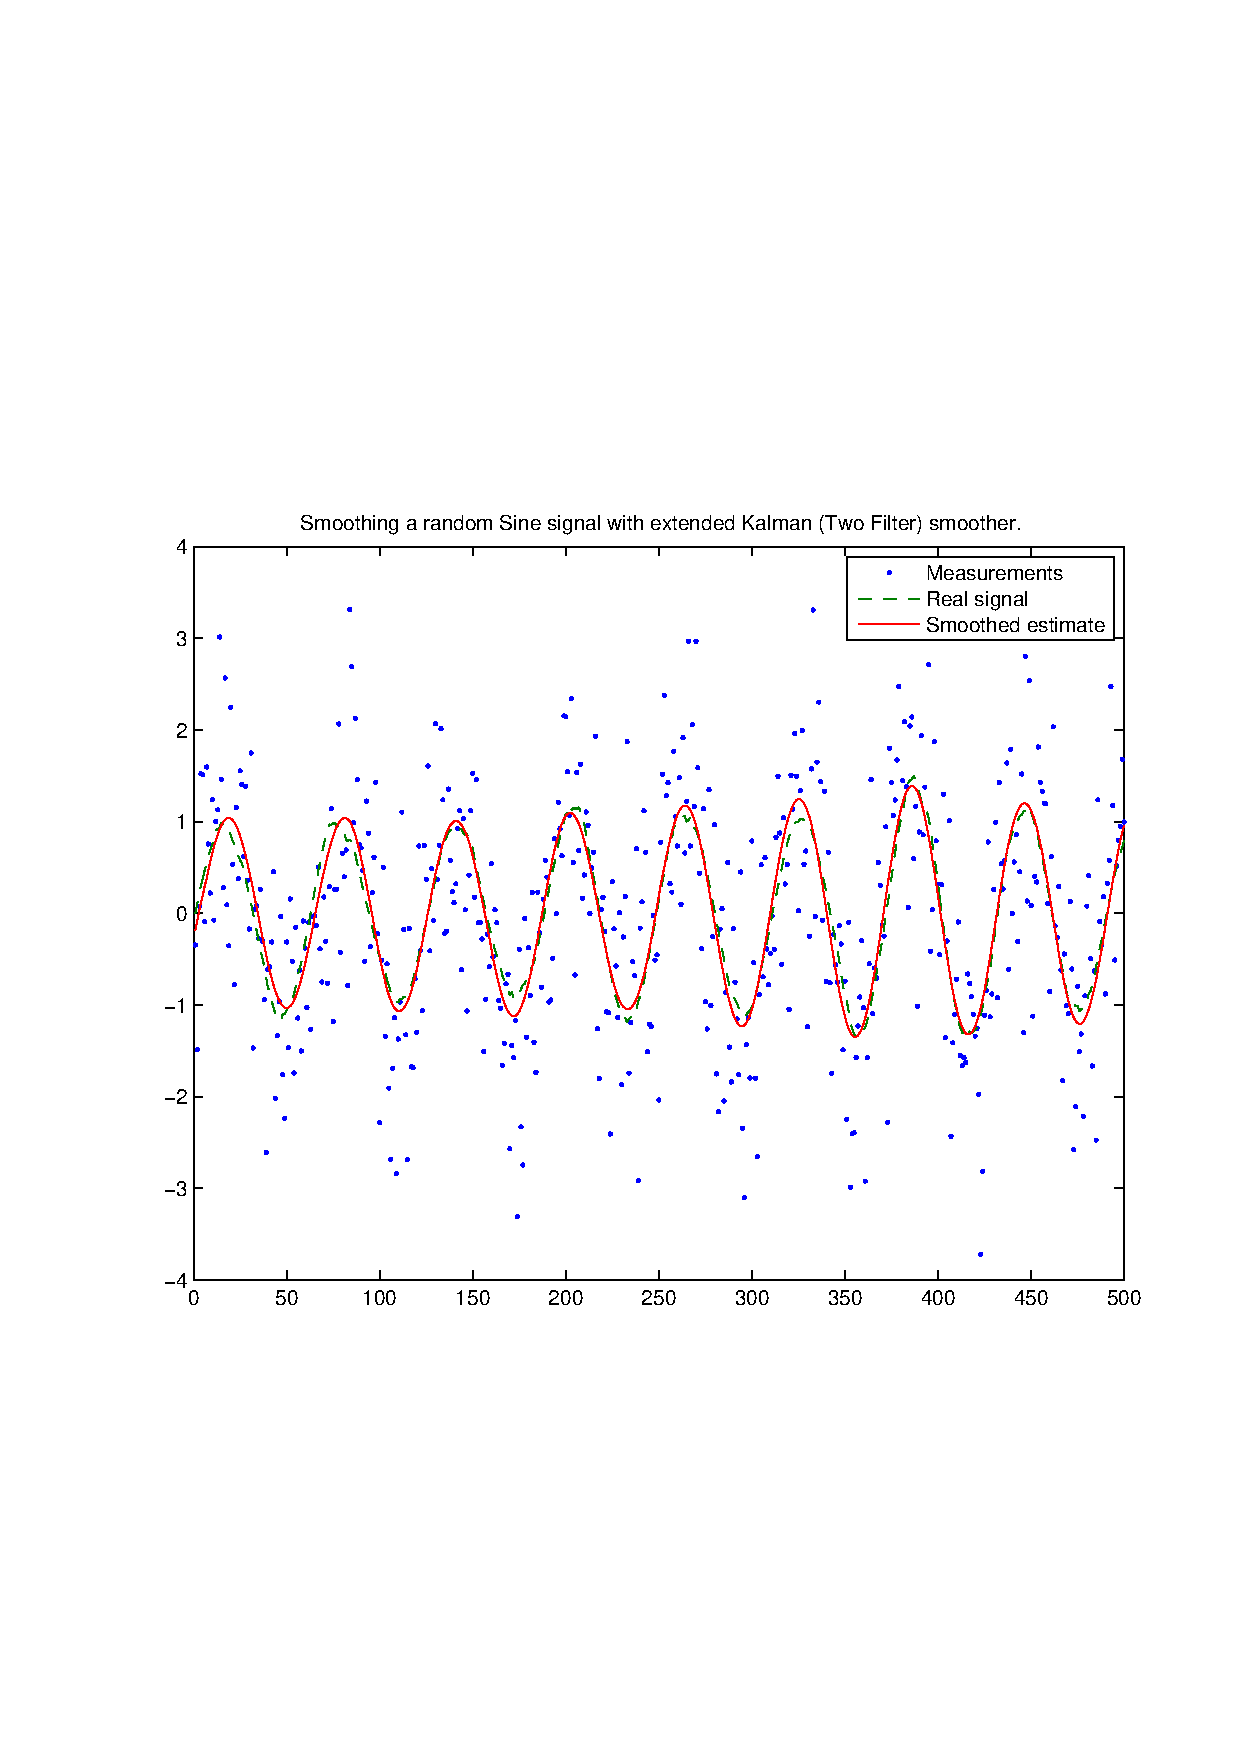
\includegraphics[width=11cm]{pics/demo2_f3}
\caption{Smoothed estimate of the sine signal using a combination of
two extended Kalman filters.}
\label{fig:example2_3}
\end{center}
\end{figure}


\begin{table}
\begin{center}
\begin{tabular}{|l|l|l|l|l|l|} \hline {\it Method}&{\it
RMSE[$\theta$]}&{\it RMSE[$\omega$]}&{\it RMSE[$a$]}& {\it
RMSE[$y$]}\\ \hline EKF1 & 0.64 & 0.53 & 0.40 & 0.24 \\ ERTS1& 0.52 &
0.31 & 0.33 & 0.15 \\ ETF1& 0.53 & 0.31 & 0.34 & 0.15 \\ EKF2 & 0.34 &
0.54 & 0.31 & 0.29 \\ ERTS2& 0.24 & 0.30 & 0.18 & 0.15 \\ ETF2& 0.24 &
0.30 & 0.18 & 0.15 \\ UKF & 0.59 & 0.56 & 0.39 & 0.27 \\ URTS & 0.45 &
0.30 & 0.30 & 0.15 \\ \hline
\end{tabular}
\caption{RMSEs of estimating the random sinusoid over 100 Monte Carlo
simulations.}
\label{table:sine_errors}
\end{center}
\end{table}



%%%%%%%%%%%%%%%%%%%%%%%%%%%%%%%%%%%%%%%%%%%%%%%%%%%%%%%%%%%%%%%%%%%%%%%%%%%%%%
%
\section{Unscented Kalman Filter}
%
%%%%%%%%%%%%%%%%%%%%%%%%%%%%%%%%%%%%%%%%%%%%%%%%%%%%%%%%%%%%%%%%%%%%%%%%%%%%%%

\subsection{Unscented Transform}

Like Taylor series based approximation presented above also the {\it
unscented transform} (UT) \citep{Julier+Uhlmann+Durrant-Whyte:1995, Julier+Uhlmann:2004, Wan+Merwe:2001} can be used for forming a Gaussian approximation to
the joint distribution of random variables $\vec{x}$ and $\vec{y}$,
which are defined with equations (\ref{eq:trans_g}). In UT we
deterministically choose a fixed number of sigma points, which capture
the desired moments (at least mean and covariance) of the original
distribution of $\vec{x}$ exactly. After that we propagate the sigma
points through the non-linear function $\vec{g}$ and estimate the
moments of the transformed variable from them.

The advantage of UT over the Taylor series based approximation is that
UT is better at capturing the higher order moments caused by the
non-linear transform, as discussed in \citep{Julier+Uhlmann:2004}. Also
the Jacobian and Hessian matrices are not needed, so the estimation
procedure is in general easier and less error-prone.
 
The unscented transform can be used to provide a Gaussian
approximation for the joint distribution of variables $\vec{x}$ and
$\vec{y}$ of the form
%
  \begin{equation}
     \begin{pmatrix} \vec{x} \\ \vec{y}
     \end{pmatrix} \sim \N\left(
     \begin{pmatrix} \vec{m} \\ \vecmu_U
     \end{pmatrix},
     \begin{pmatrix} \vec{P} & \vec{C}_U \\ \vec{C}_U^T & \mat{S}_U
     \end{pmatrix} \right).
  \end{equation}
%
The (nonaugmented) transformation is done as follows:
%
\begin{enumerate}
\item Compute the set of $2n+1$ sigma points from the columns of the
matrix $\sqrt{(n + \lambda) \, \mat{P}}$:
%
  \begin{equation}
  \begin{split} \vec{x}^{(0)} &= \vec{m} \\ \vec{x}^{(i)} &= \vec{m} +
\left[\sqrt{(n + \lambda) \, \mat{P}}\right]_i, \quad i=1,\ldots,n \\
\vec{x}^{(i)} &= \vec{m} - \left[\sqrt{(n + \lambda) \,
\mat{P}}\right]_i, \quad i=n+1,\ldots,2n
  \end{split}
  \label{eq:ut_sigmas}
  \end{equation}
%
  and the associated weights:
%
  \begin{equation}
  \begin{split} W^{(0)}_m &= \lambda / (n + \lambda) \\ W^{(0)}_c &=
\lambda / (n + \lambda) + (1 - \alpha^2 + \beta) \\ W^{(i)}_m &= 1 /
\{ 2(n + \lambda) \}, \quad i=1,\ldots,2n \\ W^{(i)}_c &= 1 / \{ 2(n +
\lambda) \}, \quad i=1,\ldots,2n.
  \end{split} \label{eq:ut_weights}
  \end{equation}
%
  Parameter $\lambda$ is a scaling parameter, which is defined as
%
  \begin{equation} \lambda = \alpha^2 \, (n + \kappa) - n.
  \end{equation}
 % 
  The positive constants $\alpha$, $\beta$ and $\kappa$ are used as
parameters of the method.

\item Propagate each of the sigma points through non-linearity as
%
  \begin{equation} \vec{y}^{(i)} = \vec{g}(\vec{x}^{(i)}), \quad
i=0,\ldots,2n.
  \label{eq:sigma_g}
  \end{equation}

\item Calculate the mean and covariance estimates for $\vec{y}$ as
%
  \begin{align} \vecmu_U &\approx \sum_{i=0}^{2n} W^{(i)}_m \,
\vec{y}^{(i)} \\ \mat{S}_U &\approx \sum_{i=0}^{2n} W^{(i)}_c \,
(\vec{y}^{(i)} - \vecmu_U) \, (\vec{y}^{(i)} - \vecmu_U)^T.
  \end{align}
  
\item Estimate the cross-covariance between $\vec{x}$ and $\vec{y}$ as
%
  \begin{equation} \mat{C}_U \approx \sum_{i=0}^{2n} W^{(i)}_c \,
(\vec{x}^{(i)} - \vec{m}) \, (\vec{y}^{(i)} - \vecmu_U)^T.
  \end{equation}
\end{enumerate}
%

The square root of positive definite matrix $\mat{P}$ is defined as
$\mat{A} = \sqrt{\mat{P}}$, where
%
\begin{equation}
%
\mat{P} = \mat{A} \mat{A}^T.
%
\end{equation}
%
To calculate the matrix $\mat{A}$ we can use, for example, lower
triangular matrix of the Cholesky factorialization, which can be
computed with built-in Matlab function \texttt{chol}. For convience,
we have provided a function (\texttt{schol}, which computes the factorialization also for
positive semidefinite matrices.


\subsection{The Matrix Form of UT}

The unscented transform described above can be written conviently in
matrix form as follows:
%
\begin{align} \mat{X} &=
      \begin{bmatrix} \vec{m} & \cdots & \vec{m} \end{bmatrix} +
\sqrt{c}
      \begin{bmatrix} \vec{0} & \sqrt{\mat{P}} & -\sqrt{\mat{P}}
      \end{bmatrix} \label{eq:ut_x1} \\ \mat{Y} &= \vec{g}(\mat{X})
\label{eq:ukf_x2} \\ \vecmu_U &= \mat{Y} \, \mat{w}_m \label{eq:ut_mu}
\\ \mat{S}_U &= \mat{Y} \, \mat{W} \, \mat{Y}^T \label{eq:ut_s} \\
\mat{C}_U &= \mat{X} \, \mat{W} \, \mat{Y}^T, \label{eq:ut_c}
\end{align}
%
where $\mat{X}$ is the matrix of sigma points, function
$\vec{g}(\cdot)$ is applied to each column of the argument matrix
separately, $c = \alpha^2 \, (n + \kappa)$, and vector $\vec{w}_m$ and
matrix $\mat{W}$ are defined as follows:
%
\begin{align} \vec{w}_m &= \begin{bmatrix} W^{(0)}_m & \cdots &
W^{(2n)}_m
   \end{bmatrix}^T \label{eq:vec_wm} \\ \mat{W} &= \left(\mat{I} -
     \begin{bmatrix} \vec{w}_m & \cdots & \vec{w}_m
     \end{bmatrix} \right) \, \nonumber \\ &\times \diag(W^{(0)}_c
\cdots W^{(2n)}_c) \, \nonumber \\ &\times \left(\mat{I} -
     \begin{bmatrix} \vec{w}_m & \cdots & \vec{w}_m
     \end{bmatrix} \right)^T.
   \label{eq:mat_w}
\end{align}
%
See (Särkkä, 2006) for proof for this.

%%%%%%%%%%%%%%%%%%%%%%%%%%%%%%%%%%%%%%%%%%%%%%%%%%%%%%%%%%%%%%%%%%%%%%%%%%%%%%
%
\subsection{Unscented Kalman Filter}
%
%%%%%%%%%%%%%%%%%%%%%%%%%%%%%%%%%%%%%%%%%%%%%%%%%%%%%%%%%%%%%%%%%%%%%%%%%%%%%%

The {\it unscented Kalman filter} (UKF) \citep{Julier+Uhlmann+Durrant-Whyte:1995, Julier+Uhlmann:2004, Wan+Merwe:2001} makes use of the {\it
unscented transform} described above to give a Gaussian approximation
to the filtering solutions of non-linear optimal filtering problems of
form (same as eq. (\ref{eq:nonlinear_prob}), but restated here for
convience)
%
\begin{equation}
\begin{split} \vec{x}_{k} &= \vec{f}(\vec{x}_{k-1},k-1) +
\vec{q}_{k-1} \\ \vec{y}_{k} &= \vec{h}(\vec{x}_{k},k) + \vec{r}_{k},
\end{split}
\end{equation}
%
where $\vec{x}_k \in \spc{R}^n$ is the state, $\vec{y}_k \in
\spc{R}^m$ is the measurement, $\vec{q}_{k-1} \sim
\N(\vec{0},\mat{Q}_{k-1})$ is the Gaussian process noise, and
$\vec{r}_{k} \sim \N(\vec{0},\mat{R}_{k})$ is the Gaussian measurement
noise.

Using the matrix form of UT described above the {\it prediction} and
{\it update} steps of the UKF can computed as follows:
%
\begin{itemize}
\item {\em Prediction:} Compute the predicted state mean $\vec{m}^-_k$
and the predicted covariance $\mat{P}^-_k$ as

%
\begin{equation}
\begin{split} \mat{X}_{k-1} &=
      \begin{bmatrix} \vec{m}_{k-1} & \cdots & \vec{m}_{k-1}
\end{bmatrix} + \sqrt{c}
      \begin{bmatrix} \vec{0} & \sqrt{\mat{P}_{k-1}} &
-\sqrt{\mat{P}_{k-1}}
      \end{bmatrix} \\ \hat{\mat{X}}_{k} &= \vec{f}(\mat{X}_{k-1},k-1)
\\ \vec{m}^-_{k} &= \hat{\mat{X}}_{k} \, \mat{w}_m \\ \mat{P}^-_{k} &=
\hat{\mat{X}}_{k} \, \mat{W} \, [ \hat{\mat{X}}_{k} ]^T +
\mat{Q}_{k-1}.
\end{split} \label{eq:ukf1_predict}
\end{equation}
%
\item {\em Update:} Compute the predicted mean $\vecmu_k$ and
covariance of the measurement $\mat{S}_k$, and the cross-covariance of
the state and measurement $\mat{C}_k$:
%
\begin{equation}
\begin{split} \mat{X}^-_k &=
      \begin{bmatrix} \vec{m}^-_k & \cdots & \vec{m}^-_k \end{bmatrix}
+ \sqrt{c}
      \begin{bmatrix} \vec{0} & \sqrt{\mat{P}^-_k} &
-\sqrt{\mat{P}^-_k}
      \end{bmatrix} \\ \mat{Y}^-_k &= \vec{h}(\mat{X}^-_k,k) \\
\vec{\mu}_k &= \mat{Y}^-_k \, \mat{w}_m \\ \mat{S}_k &= \mat{Y}^-_k \,
\mat{W} \, [\mat{Y}^-_k]^T + \mat{R}_{k} \\ \mat{C}_k &= \mat{X}^-_k
\, \mat{W} \, [\mat{Y}^-_k]^T.
\end{split}
\label{eq:ukf1_update1}
\end{equation}
%

Then compute the filter gain $\mat{K}_k$ and the updated state mean
$\vec{m}_k$ and covariance $\mat{P}_k$:
%
\begin{equation}
\begin{split} \mat{K}_k &= \mat{C}_k \, \mat{S}_k^{-1} \\ \vec{m}_k &=
\vec{m}^-_k + \mat{K}_k \, \left[ \vec{y}_k - \vecmu_k \right] \\
\mat{P}_k &= \mat{P}^-_k - \mat{K}_k \, \mat{S}_k \, \mat{K}_k^T.
\end{split}
\label{eq:ukf1_update2}
\end{equation}
\end{itemize}

The prediction and update steps of the nonaugmented UKF can be
computed with functions \texttt{ukf\_predict1} and
\texttt{ukf\_update1}, respectively.

\subsection{Augmented UKF}

It is possible to modify the UKF procedure described above by forming
an {\it augmented} state variable, which concatenates the state and
noise components together, so that the effect of process and
measurement noises can be used to better capture the odd-order moment
information. This requires that the sigma points generated during the
predict step are also used in the update step, so that the effect of
noise terms are truly propagated through the nonlinearity \citep{Wu+Hu+Wu+Hu:2005}. If, however, we generate new sigma points in the update step
the augmented approach give the same results as the nonaugmented, if
we had assumed that the noises were additive. If the noises are not
additive the augmented version should produce more accurate estimates
than the nonaugmented version, even if new sigma points are created
during the update step.

The {\it prediction} and {\it update} steps of the augmented UKF in
matrix form are as follows:
%
\begin{itemize}
\item {\em Prediction:} Form a matrix of sigma points of the augmented
state variable \\$\tilde{\vec{x}}_{k-1} =
\begin{bmatrix} \vec{x}_{k-1}^T & \vec{q}_{k-1}^T & \vec{r}_{k-1}^T
\end{bmatrix}^T$ as
%
\begin{equation}
%
\mat{\tilde{X}}_{k-1} =
   \begin{bmatrix} \tilde{\vec{m}}_{k-1} & \cdots &
\tilde{\vec{m}}_{k-1} \end{bmatrix} + \sqrt{c}
   \begin{bmatrix} \vec{0} & \sqrt{\tilde{\mat{P}}_{k-1}} &
-\sqrt{\tilde{\mat{P}}_{k-1}}
   \end{bmatrix},
%
\label{eq:ukf2_predict1}
\end{equation}
%
where
%
\begin{equation}
%
\tilde{\vec{m}}_{k-1} = \begin{bmatrix} \vec{m}_{k-1}^T & \vec{0} &
\vec{0} \end{bmatrix}^T
%
\text{ and }
%
\tilde{\mat{P}}_{k-1} =
\begin{bmatrix} \mat{P_{k-1}} & \mat{0} & \mat{0} \\ \mat{0} &
\mat{Q}_{k-1} & \mat{0} \\ \mat{0} & \mat{0} & \mat{R}_{k-1} \\
\end{bmatrix}.
%
\label{eq:ukf2_predict2}
\end{equation}

Then compute the predicted state mean $\vec{m}^-_k$ and the predicted
covariance $\mat{P}^-_k$ as
%
\begin{equation}
\begin{split} \hat{\mat{X}}_{k} &=
\vec{f}(\mat{X^x}_{k-1},\mat{X^q}_{k-1},k-1) \\ \vec{m}^-_{k} &=
\hat{\mat{X}}_{k} \, \mat{w}_m \\ \mat{P}^-_{k} &= \hat{\mat{X}}_{k}
\, \mat{W} \, [ \hat{\mat{X}}_{k} ]^T,
\end{split}
\label{eq:ukf2_predict3}
\end{equation}
%
where we have denoted the components of sigma points which correspond
to actual state variables and process noise with matrices
$\mat{X}^x_{k-1}$ and $\mat{X}^q_{k-1}$, respectively. The state
transition function $\vec{f}$ is also augmented to incorporate the
effect of process noise, which is now passed to the function as a
second parameter. In additive noise case the process noise is directly
added to the state variables, but other forms of noise effect are now
also allowed.

%
\item {\em Update:} Compute the predicted mean $\vecmu_k$ and
covariance of the measurement $\mat{S}_k$, and the cross-covariance of
the state and measurement $\mat{C}_k$:
%
\begin{equation}
\begin{split} \mat{Y}^-_k &=
\vec{h}(\hat{\mat{X}}_k,\mat{X}^r_{k-1},k) \\ \vec{\mu}_k &=
\mat{Y}^-_k \, \mat{w}_m \\ \mat{S}_k &= \mat{Y}^-_k \, \mat{W} \,
[\mat{Y}^-_k]^T \\ \mat{C}_k &= \hat{\mat{X}}_k \, \mat{W} \,
[\mat{Y}^-_k]^T,
\end{split}
\label{eq:ukf2_update1}
\end{equation}
%
where we have denoted the component of sigma points corresponding to
measurement noise with matrix $\mat{X}^r_{k-1}$. Like the state
transition function $\vec{f}$ also the measurement function $\vec{h}$
is now augmented to incorporate the effect of measurement noise, which
is passed as a second parameter to the function.

Then compute the filter gain $\mat{K}_k$ and the updated state mean
$\vec{m}_k$ and covariance $\mat{P}_k$:
%
\begin{equation}
\begin{split} \mat{K}_k &= \mat{C}_k \, \mat{S}_k^{-1} \\ \vec{m}_k &=
\vec{m}^-_k + \mat{K}_k \, \left[ \vec{y}_k - \vecmu_k \right] \\
\mat{P}_k &= \mat{P}^-_k - \mat{K}_k \, \mat{S}_k \, \mat{K}_k^T.
\end{split}
\label{eq:ukf2_update2}
\end{equation}
\end{itemize}
%

Note that nonaugmented form UKF is computationally less demanding than
augmented form UKF, because it creates a smaller number of sigma
points during the filtering procedure. Thus, the usage of the
nonaugmented version should be preferred over the augmented
version, if the propagation of noise terms doesn't improve the
accuracy of the estimates.

The prediction and update steps of the augmented UKF can be computed
with functions \texttt{ukf\_predict3} and \texttt{ukf\_update3},
respectively. These functions concatenates the state variables,
process and measurements noises to the augmented variables, as was
done above.

It is also possible to separately concatenate only the state variables
and process noises during prediction step and state variables and
measurement noises during update step. Filtering solution based on
this formulation can be computed with functions \texttt{ukf\_predict2}
and \texttt{ukf\_update2}. However, these functions create new sigma
points during the update step in addition to ones created during
prediction step, and hence the higher moments might not get captured
so effectively in cases, where the noise terms are additive.


%%%%%%%%%%%%%%%%%%%%%%%%%%%%%%%%%%%%%%%%%%%%%%%%%%%%%%%%%%%%%%%%%%%%%%%%%%%%%%
%
\subsection{Unscented Kalman Smoother}
%
%%%%%%%%%%%%%%%%%%%%%%%%%%%%%%%%%%%%%%%%%%%%%%%%%%%%%%%%%%%%%%%%%%%%%%%%%%%%%%

The Rauch-Rung-Striebel type smoother using the unscented
transformation \citep{Sarkka:2008} can be used for computing a Gaussian
approximation to the smoothing distribution of the step $k$:
%
\begin{equation}
%
p(\vec{x}_k|\vec{y}_{1:T}) \sim N(\vec{x}_k|\vec{m}_k^s,\mat{P}_k^s),
%
\end{equation}
% 
as follows (using again the matrix form):
%
\begin{itemize}
%
\item Form a matrix of sigma points of the augmented state variable
$\tilde{\vec{x}}_{k-1} =
\begin{bmatrix} \vec{x}_{k-1}^T & \vec{q}_{k-1}^T \end{bmatrix}^T$ as
%
\begin{equation}
%
\mat{\tilde{X}}_{k-1} =
   \begin{bmatrix} \tilde{\vec{m}}_{k-1} & \cdots &
\tilde{\vec{m}}_{k-1} \end{bmatrix} + \sqrt{c}
   \begin{bmatrix} \vec{0} & \sqrt{\tilde{\mat{P}}_{k-1}} &
-\sqrt{\tilde{\mat{P}}_{k-1}}
   \end{bmatrix},
%
\label{eq:urts1}
\end{equation}
%
where
%
\begin{equation}
%
\tilde{\vec{m}}_{k-1} = \begin{bmatrix} \vec{m}_{k-1}^T & \vec{0}
\end{bmatrix}^T
%
\text{ and }
%
\tilde{\mat{P}}_{k-1} =
\begin{bmatrix} \mat{P_{k-1}} & \mat{0} \\ \mat{0} & \mat{Q}_{k-1} \\
\end{bmatrix}.
\label{eq:urts2}
\end{equation}
%
\item Propagate the sigma points through the dynamic model:
%
\begin{equation}
%
\tilde{\mat{X}}_{k+1}^- =
\vec{f}(\tilde{\mat{X}}^x_{k},\tilde{\mat{X}}^q_{k},k),
%
\label{eq:urts3}
\end{equation}
% 
where $\tilde{\mat{X}}^x_{k}$ and $\tilde{\mat{X}}^q_{k}$ denotes the
parts of sigma points, which correspond to $\vec{x}_k$ and
$\vec{q}_k$, respectively.

\item Compute the predicted mean $\vec{m}^-_{k+1}$, covariance
$\mat{P}^-_{k+1}$ and cross-covariance $\mat{C}_{k+1}$:
\begin{equation}
\begin{split} \vec{m}^-_{k+1} &= \tilde{\mat{X}}_{k+1}^{-x} \,
\mat{w}_m \\ \mat{P}^-_{k+1} &= \tilde{\mat{X}}_{k+1}^{-x} \, \mat{W}
\, [\tilde{\mat{X}}_{k+1}^{-x}]^T \\ \mat{C}_{k+1} &=
\tilde{\mat{X}}_{k+1}^{-x} \, \mat{W} \, [\tilde{\mat{X}}^x_{k}]^T,
\end{split}
\label{eq:urts4}
\end{equation}
%
where $\tilde{\mat{X}}_{k+1}^{-x}$ denotes the part of propagated
sigma points $\tilde{\mat{X}}_{k+1}^-$, which corresponds to
$\vec{x}_k$.
%
\item Compute the smoother gain $\mat{D}_k$, the smoothed mean
$\vec{m}_k^s$ and the covariance $\mat{P}_k^s$:
\begin{equation}
\begin{split} \mat{D}_k & = \mat{C}_{k+1} [\mat{P}_{k+1}^-]^{-1} \\
\vec{m}_k^s & = \vec{m}_k + \mat{D}_k [\vec{m}^s_{k+1} -
\vec{m}_{k+1}^-] \\ \mat{P}_k^s & = \mat{P}_k + \mat{D}_k
[\mat{P}^s_{k+1} - \mat{P}_{k+1}^-] \mat{D}_k^T.
\end{split}
\label{eq:urts5}
\end{equation}

\end{itemize}
%

The smoothing solution of this augmented type RTS smoother can be
computed with function \texttt{urts\_smooth2}. Also a nonaugmented
version of this type smoother has been implemented, and a smoothing
solution with that can be computed with function
\texttt{urts\_smooth1}.



\newpage \clearpage

%%%%%%%%%%%%%%%%%%%%%%%%%%%%%%%%%%%%%%%%%%%%%%%%%%%%%%%%%%%%%%%%%%%%%%%%%%%%%%
%
   % Cubature Methods in non-linear Kalman filtering and smoothing
%
   % These sections were added to the toolbox documentation originally in summer 2010.
%    
   % Arno Solin, 2010
%
%%%%%%%%%%%%%%%%%%%%%%%%%%%%%%%%%%%%%%%%%%%%%%%%%%%%%%%%%%%%%%%%%%%%%%%%%%%%%%




%%%%%%%%%%%%%%%%%%%%%%%%%%%%%%%%%%%%%%%%%%%%%%%%%%%%%%%%%%%%%%%%%%%%%%%%%%%%%%
%
\section{Gauss-Hermite Kalman Filter}
%
%%%%%%%%%%%%%%%%%%%%%%%%%%%%%%%%%%%%%%%%%%%%%%%%%%%%%%%%%%%%%%%%%%%%%%%%%%%%%%

\subsection{Gauss-Hermite Cubature Transformation}

To unify many of the filter variants, handling the non-linearities may be brought together to a common formulation. In Gaussian optimal filtering --- also called assumed density filtering --- the filtering equations follow the assumption that the filtering distributions are indeed Gaussian \citep{Maybeck:1982, Ito+Xiong:2000}. %\citep{maybeck1982,ito2000}.

Using this setting the linear Kalman filter equations can now be adapted to the non-linear state-space model. Desired moments (at least mean and covariance) of the original distribution of $\vec{x}$ can be captured exactly by calculating the integrals

\begin{align}%
\begin{split} \label{eqCh2integral1}
    \bmu_U &= \int \vec{f}(\vec{x})\,\N(\vec{x} \mid \vec{m},\,\vec{P}) \diff \vec{x} \\
    \vec{S}_U &= \int \left(\vec{f}(\vec{x}) - \bmu_U\right) \left(\vec{f}(\vec{x}) - \bmu_U\right)\T 
     \times \N(\vec{x} \mid \vec{m},\,\vec{P}) \diff \vec{x}.
\end{split}%
\end{align}

These integrals can be evaluated with practically any analytical or numerical integration method. The Gauss--Hermite quadrature rule is a one-dimensional weighted sum approximation method for solving special integrals of the previous form in a Gaussian kernel with an infinite domain. More specifically the Gauss--Hermite quadrature can be applied to integrals of form

\begin{equation} \label{eqGaussHermite1D}
    \int_{-\infty}^\infty f(x)\,\exp(-x^2) \diff x \approx \sum_{i=1}^m w_i\,f(x_i),
\end{equation}

\noindent%
where $x_i$ are the sample points and $w_i$ the associated weights to use for the approximation. The sample points $x_i, i=1,\ldots,m,$ are roots of special orthogonal polynomials, namely the Hermite polynomials. The Hermite polynomial of degree $p$ is denoted with $H_p(x)$ \citep[see][for details]{Abramowitz+Stegun:1964}. The weights $w_i$ are given by

\begin{equation} \label{eqGaussHermiteWeights}
    w_i = \frac{2^{p-1}p!\sqrt{\pi}}{p^2[H_{p-1}(x_i)]^2}.
\end{equation}

The univariate integral approximation needs to be extended to be able to suit the multivariate case. As \citet{Wu+Hu+Wu+Hu:2006}  argue, the most natural approach to grasp a multiple integral is to treat it as a sequence of nested univariate integrals and then use a univariate quadrature rule repeatedly. To extend this one-dimensional integration method to multi-dimensional integrals of form

\begin{equation} \label{eqGaussHermiteND}
    \int_{\mathbb{R}^n} f(\vec{x})\,\exp(-\vec{x}\T\vec{x}) \diff \vec{x} \approx \sum_{i=1}^m w_i\,f(\vec{x}_i),
\end{equation}

\noindent%
we first simply form the one-dimensional quadrature rule with respect to the first dimension, then with respect to the second dimension and so on \citep{Cools:1997}. We get the multidimensional Gauss--Hermite cubature rule by writing

\begin{align*}
    & \sum_{i_1} w_{i_1} \int f(x_1^{i_1},x_2, \ldots, x_n) \exp(-x_2^2 -x_3^2 \ldots -x_n^2) \diff x_2 \ldots \diff x_n \\
    =& \sum_{i_1,i_2} w_{i_1} w_{i_2} \int f(x_1^{i_1},x_2^{i_2}, \ldots, x_n) \exp(-x_3^2 \ldots -x_n^2) \diff x_3 \ldots \diff x_n \\
    =& \sum_{i_1,i_2,\ldots,i_n} w_{i_1} w_{i_2} \cdots  w_{i_n} \, f(x_1^{i_1},x_2^{i_2}, \ldots, x_n^{i_n}),
\end{align*}

\noindent%
which is basically what we wanted in Equation~\eqref{eqGaussHermiteND}. This gives us the \emph{product rule} that simply extends the one-dimensional quadrature point set of $p$ points in one dimension to a lattice of $p^n$ cubature points in $n$ dimensions. The weights for these Gauss--Hermite cubature points are calculated by the product of the corresponding one-dimensional weights.

Finally, by making a change of variable $\vec{x} = \sqrt{2}\sqrt{\vec{\Sigma}} + \bmu$ we get the Gauss--Hermite weighted sum approximation for a multivariate Gaussian integral, where $\bmu$ is the mean and $\bSigma$ is the covariance of the Gaussian. The square root of the covariance matrix, denoted $\sqrt{\bSigma}$, is  a matrix such that $\bSigma = \sqrt{\bSigma}\sqrt{\bSigma}\T$.

\begin{equation}
    \int_{\mathbb{R}^n} \vec{f}(\vec{x})\,\N(\vec{x} \mid \bmu,\, \vec{\Sigma})\diff\vec{x} 
    \approx \sum_{i_1, i_2, \ldots, i_n} w_{i_1, i_2, \ldots, i_n} \, f\left(\sqrt{\vec{\Sigma}}\, \boldsymbol{\xi}_{i_1, i_2, \ldots, i_n} +\bmu \right),
\end{equation}

\noindent%
where the weight $w_{i_1, i_2, \ldots, i_n} = {1 \over \pi^{n/2}} w_{i_1} \cdot w_{i_2} \cdots w_{i_n}$ is given by using the one-dimensional weights, and the points are given by the Cartesian product $\boldsymbol{\xi}_{i_1, i_2, \ldots, i_n} = \sqrt{2} \, (x_{i_1}, x_{i_2}, \ldots, x_{i_n})$, where $x_i$ is the $i$th one-dimensional quadrature point. 

%% The curse of dimensionality
The extension of the Gauss--Hermite quadrature rule to an $n$-dimensional cubature rule by using the product rule lattice approach yields a rather good numerical integration method that is exact for monomials $\prod_{i=1}^n x_i^{k_i} $ with $k_i \leq 2p - 1$ \citep{Wu+Hu+Wu+Hu:2006}. However, the number of cubature points grows exponentially as the number of dimensions increases. Due to this flaw the rule is not practical in applications with many dimensions. This problem is called the \emph{curse of dimensionality}.












%%%%%%%%%%%%%%%%%%%%%%%%%%%%%%%%%%%%%%%%%%%%%%%%%%%%%%%%%%%%%%%%%%%%%%%%%%%%%%
%
\subsection{Gauss-Hermite Kalman Filter}
%
%%%%%%%%%%%%%%%%%%%%%%%%%%%%%%%%%%%%%%%%%%%%%%%%%%%%%%%%%%%%%%%%%%%%%%%%%%%%%%

The Gauss--Hermite Kalman filter (GHKF) algorithm of degree $p$ is presented below. At time $k = 1,\ldots,T$ assume the posterior density function $ p(\vec{x}_{k-1} \mid \vec{y}_{k-1}) = \N(\vec{m}_{k-1 \mid k-1},\vec{P}_{k-1 \mid k-1})$ is known.


%% The Prediction step
\textbf{Prediction step:}

\begin{enumerate}

  \item Find the roots $x_i, i=1,\ldots,p$, of the Hermite polynomial $H_p(x)$.%

  \item Calculate the corresponding weights%
%
   $$ w_i = \frac{2^{p-1}p!}{p^2[H_{p-1}(x_i)]^2}. $$

  \item Use the product rule to expand the points to a $n$-dimensional lattice of $p^n$ points $\boldsymbol{\xi}_i, i=1,\ldots,p^n,$ with corresponding weights. 

  \item Propagate the cubature points. The matrix square root is the lower triangular cholesky factor.%
%
    $$ \vec{X}_{i,k-1 \mid k-1} = \sqrt{2 \vec{P}_{k-1 \mid k-1}} \boldsymbol{\xi}_i + \vec{m}_{k-1 \mid k-1}$$

  \item Evaluate the cubature points with the dynamic model function%
%
    $$ \vec{X}_{i,k \mid k-1}^* = \vec{f}(\vec{X}_{i,k-1 \mid k-1}). $$

  \item Estimate the predicted state mean%
%
    $$ \vec{m}_{k \mid k-1}  = \sum_{i=1}^{p^n} w_i \vec{X}_{i,k \mid k-1}^*. $$

  \item Estimate the predicted error covariance%
%
    $$ \vec{P}_{k \mid k-1} = \sum_{i=1}^{p^n} w_i \vec{X}_{i,k \mid k-1}^* \vec{X}_{i,k \mid k-1}^{*\mathsf{T}} - \vec{m}_{k \mid k-1} \vec{m}_{k \mid k-1}\T + \vec{Q}_{k-1}.$$ 

\end{enumerate}


%% The Update step
\noindent
\textbf{Update step:}

\begin{enumerate}

  \item Repeat steps 1--3 from earlier to get the $p^n$ cubature points and their weights. 

  \item Propagate the cubature points.%
%
    $$ \vec{X}_{i,k \mid k-1} = \sqrt{2 \vec{P}_{k \mid k-1}} \boldsymbol{\xi}_i + \vec{m}_{k \mid k-1}$$

  \item Evaluate the cubature points with the help of the measurement model function%
%
    $$ \vec{Y}_{i,k \mid k-1} = \vec{h}(\vec{X}_{i,k \mid k-1}). $$

  \item Estimate the predicted measurement%
%
    $$ \vec{\hat{y}}_{k \mid k-1} = \sum_{i=1}^{p^n} w_i \vec{Y}_{i,k \mid k-1}. $$

  \item Estimate the innovation covariance matrix%
%
    $$ \vec{S}_{k \mid k-1} = \sum_{i=1}^{p^n} w_i \vec{Y}_{i,k \mid k-1} \vec{Y}_{i,k \mid k-1}\T - \vec{\hat{y}}_{k \mid k-1} \vec{\hat{y}}_{k \mid k-1}\T + \vec{R}_k. $$
    
  \item Estimate the cross-covariance matrix%
%
    $$ \vec{P}_{xy,k \mid k-1} = \sum_{i=1}^{p^n} w_i \vec{X}_{i,k-1 \mid k-1} \vec{Y}_{i,k \mid k-1}\T - \vec{m}_{k \mid k-1} \vec{\hat{y}}_{k \mid k-1}\T.$$ 

  \item Calculate the Kalman gain term and the smoothed state mean and covariance%
%
  \begin{align*}
     \vec{K}_k = \vec{P}_{xy,k \mid k-1} \vec{S}_{k \mid k-1}^{-1} \\
     \vec{m}_{k \mid k} = \vec{m}_{k \mid k-1} + \vec{K}_k(\vec{y}_k - \vec{\hat{y}}_{k \mid k-1}) \\
     \vec{P}_{k \mid k} = \vec{P}_{k \mid k-1} - \vec{K}_k \vec{P}_{yy,k \mid k-1} \vec{K}_k\T. 
  \end{align*}
\end{enumerate}












%%%%%%%%%%%%%%%%%%%%%%%%%%%%%%%%%%%%%%%%%%%%%%%%%%%%%%%%%%%%%%%%%%%%%%%%%%%%%%
%
\subsection{Gauss-Hermite Kalman Smoother}
%
%%%%%%%%%%%%%%%%%%%%%%%%%%%%%%%%%%%%%%%%%%%%%%%%%%%%%%%%%%%%%%%%%%%%%%%%%%%%%%

The Gauss--Hermite Rauch--Tung--Striebel smoother (GHRTS) algorithm \citep{Sarkka+Hartikainen:2010} of degree $p$ is presented below. Assume the filtering result mean $\vec{m}_{k \mid k}$ and covariance $\vec{P}_{k \mid k}$ are known together with the smoothing result $ p(\vec{x}_{k+1} \mid \vec{y}_{1:T}) = \N(\vec{m}_{k+1 \mid T},\vec{P}_{k+1 \mid T})$.


%% Smoothing
\begin{enumerate}

  \item Find the roots $x_i, i=1,\ldots,p$, of the Hermite polynomial $H_p(x)$.%

  \item Calculate the corresponding weights%
%
   $$ w_i = \frac{2^{p-1}p!}{p^2[H_{p-1}(x_i)]^2}. $$

  \item Use the product rule to expand the points to a $n$-dimensional lattice of $p^n$ points $\boldsymbol{\xi}_i, i=1,\ldots,p^n,$ with corresponding weights.  

  \item Propagate the cubature points%
%
    $$ \vec{X}_{i,k \mid k} = \sqrt{2 \vec{P}_{k \mid k}} \boldsymbol{\xi}_i + \vec{m}_{k \mid k}. $$

  \item Evaluate the cubature points with the dynamic model function%
%
    $$ \vec{X}_{i,k+1 \mid k}^* = \vec{f}(\vec{X}_{i,k \mid k}). $$

  \item Estimate the predicted state mean%
%
    $$ \vec{m}_{k+1 \mid k}  = \sum_{i=1}^{p^n} w_i \vec{X}_{i,k+1 \mid k}^*. $$

  \item Estimate the predicted error covariance%
%
    $$ \vec{P}_{k+1 \mid k} = \sum_{i=1}^{p^n} w_i \vec{X}_{i,k+1 \mid k}^* \vec{X}_{i,k+1 \mid k}^{*\mathsf{T}} - \vec{m}_{k+1 \mid k} \vec{m}_{k+1 \mid k}\T + \vec{Q}_{k}.$$

  \item Estimate the cross-covariance matrix%
%
    $$ \vec{D}_{k , k+1} = {1 \over 2 n} \sum_{i=1}^{2 n} \big(\vec{X}_{i,k \mid k} - \vec{m}_{k \mid k}\big) \\ \big(\vec{X}_{i,k+1 \mid k}^* - \vec{m}_{k+1 \mid k}\big)\T. $$ 

  \item Calculate the gain term and the smoothed state mean and covariance%
%
  \begin{align*}
     \vec{C}_k &= \vec{D}_{k , k+1} \vec{P}_{k+1 \mid k}^{-1} \\
     \vec{m}_{k \mid T} &= \vec{m}_{k \mid k} + \vec{C}_k(\vec{m}_{k+1 \mid T} - \vec{m}_{k+1 \mid k}) \\
     \vec{P}_{k \mid T} &= \vec{P}_{k \mid k} + \vec{C}_k (\vec{P}_{k+1 \mid T} - \vec{P}_{k+1 \mid k}) \vec{C}_k\T.
  \end{align*}

\end{enumerate}














\newpage
%%%%%%%%%%%%%%%%%%%%%%%%%%%%%%%%%%%%%%%%%%%%%%%%%%%%%%%%%%%%%%%%%%%%%%%%%%%%%%
%
\section{Cubature Kalman Filter}
%
%%%%%%%%%%%%%%%%%%%%%%%%%%%%%%%%%%%%%%%%%%%%%%%%%%%%%%%%%%%%%%%%%%%%%%%%%%%%%%

\subsection{Spherical-Radial Cubature Transformation}

As in the Gauss--Hermite cubature rule based Gauss--Hermite transformation the spherical--radial cubature transformation utilizes the assumed density approach. The integrals that need to be solved are the same Gaussian integrals, but the numerical integration method differs from the product rule based Gauss--Hermite method.

The curse of dimensionality causes all product rules to be highly ineffective in integration regions with multiple dimensions. To mitigate this issue, we may seek alternative approaches to solving Gaussian integrals. The non-product rules differ from product based solutions by choosing the evaluation points directly from the domain of integration. That is, the points are not simply duplicated from one dimension to multiple dimensions, but directly chosen from the whole domain.

We constrain our interest to integrals of form

\begin{equation} \label{eqAlmostgaussian}
    \operatorname{I}(\vec{f}) = \int_{\mathbb{R}^n} f(\vec{x})\exp(-\vec{x}\T\vec{x})\diff\vec{x}.
\end{equation}

\noindent%
We make a change of variable from $\vec{x} \in \mathbb{R}^n$ to spherical coordinates, which lets us split the integrand into two: a radial integral

\begin{equation} \label{eqRadial}
    \operatorname{I}(\vec{f}) = \int_0^\infty \operatorname{S}(r) \, r^{n-1} \exp(-r^2) \diff r,
\end{equation}

\noindent%
and a spherical integral

\begin{equation} \label{eqSpherical}
    \operatorname{S}(r) = \int_{S_n} f(r\vec{y}) \diff\sigma(\vec{y}).
\end{equation}

The spherical integral~\eqref{eqSpherical} can be seen as a spherical integral with the unit weighting function $w(\vec{y}) \equiv 1$. Now the spherical and radial integral may be interpreted separately and computed with the spherical cubature rule and the Gaussian quadrature rule respectively.




In a fully symmetric cubature point set equally weighted points are symmetrically distributed around origin. A point $\vec{u}$ is called the \emph{generator} of such a set, if for the components of $\vec{u} = \begin{pmatrix} u_1,u_2,\ldots,u_r,0,\ldots,0 \end{pmatrix} \in \mathbb{R}^n$, $u_i \geq u_{i+1} > 0,\, i= 1,2,\ldots,(r-1)$. For example, we may denote $[\vec{1}] \in \mathbb{R}^2$ to represent the cubature point set 

\begin{equation*}
\left\{ 
  \begin{pmatrix}  1 \\  0  \end{pmatrix},
  \begin{pmatrix}  0 \\  1  \end{pmatrix},
  \begin{pmatrix} -1 \\  0  \end{pmatrix},
  \begin{pmatrix}  0 \\ -1  \end{pmatrix}
 \right\},
\end{equation*}

\noindent%
where the generator is $\begin{pmatrix} 1 & 0 \end{pmatrix}\T$.

To find the unknowns of a cubature rule of degree $d$, a set of moment equations have to be solved. This, however, may not be a simple task with increasing dimensions and polynomial degree. To reduce the size of the system of equations or the number of needed cubature points \citep{Arasaratnam+Haykin:2009} use the \emph{invariant theory} proposed by Sobolev \citep[see][]{Cools:1997}. The invariant theory discusses how to simplify the structure of a cubature rule by using the symmetries of the region of integration. The unit hypercube, the unit  hypersphere and the unit simplex all contain some symmetry.

Due to invariance theory \citep{Cools:1997} the integral~\eqref{eqSpherical} can be approximated by a third-degree spherical cubature rule that gives us the sum

\begin{equation} \label{eqSphericalSum}
    \int_{S_n} f(r\vec{y}) \diff\sigma(\vec{y}) \approx w \sum_{i=1}^{2n}\vec{f}([\vec{u}]_i).
\end{equation}

\noindent%
The point set $[\vec{u}]$ is invariant under permutations and sign changes, which means that a number of $2n$ cubature points are sufficient to approximate the integral. For the above choice, the monomials $y_1^{d_1}y_2^{d_2}\cdots y_n^{d_n}$, with the sum $\sum_{i=1}^n d_i$ being an odd integer, are integrated exactly.

To make this rule exact for all monomials up to degree three, we have to require the rule to be exact for the even dimensions $\sum_{i=1}^n d_i = \{0,2\}$. This can be accomplished by solving the unknown parameters for a monomial function of order $n=0$ and equivalently for a monomial function of order $n=2$. We consider the two functions $\vec{f}(\cdot)$ to be of form $\vec{f}(\vec{y})=1$, and $\vec{f}(\vec{y})=y_1^2$. This yields the pair of equations \citep{Arasaratnam:2009}.

\begin{align*}
    \vec{f}(\vec{y})&=1 :& 2nw &= \int_{S_n} \diff\sigma(\vec{y}) = A_n \\
    \vec{f}(\vec{y})&=y_1^2 :& 2wu^2 &= \int_{S_n} y_1^2 \diff\sigma(\vec{y}) = \frac{1}{n} A_n,
\end{align*}

\noindent%
where $A_n$ is the surface area of the $n$-dimensional unit sphere. Solving these equations yields $u^2 = 1$ and $w = \frac{A_n}{2n}$. Therefore the cubature points can be chosen so that they are located at the intersection of the unit sphere and its axes.







The radial integral defined in Equation~\eqref{eqRadial} can be transformed to a familiar Gauss--Laguerre form (see Abramowitz and Stegun, 1964) by making another change of variable, $t=r^2$, which yields

\begin{equation} \label{eqRadialChange}
    \int_0^\infty \operatorname{S}(r) \, r^{n-1} \exp(-r^2) \diff r = 
    {1 \over 2} \int_0^\infty \operatorname{\tilde{S}}(t) \, t^{{n \over 2}-1} \exp(-t) \diff t = \sum_{i=1}^m w_i \operatorname{\tilde{S}}(t_i),
\end{equation}

where $t_i$ is the $i$th root of \emph{Laguerre polynomial} $L_m(t)$ and the weights $w_i$ are given by \citep{Abramowitz+Stegun:1964} 

  $$w_i = {t_i \over (m+1)^2(L_{m+1}(t_i))^2}.$$

\noindent%
A first-degree Gauss--Laguerre rule is exact for $\operatorname{\tilde{S}}(t)=\{1,t\}$ (or equivalently $\operatorname{S}(r)=\{1,r^2\}$). Due to the properties of the spherical cubature rule presented earlier, the combined spherical--radial rule vanishes by symmetry for all odd degree polynomials. Hence, to have the spherical--radial rule to be exact for all polynomials up to degree three in $\vec{x} \in \mathbb{R}^n$ it is sufficient to use the first degree Gauss--Laguerre rule of the form \citep{Arasaratnam:2009}

\begin{equation*}
    \int_0^\infty \operatorname{\tilde{S}_i}(t) \, t^{{n \over 2}-1} \exp(-t) \diff t = 
    w_1 \operatorname{\tilde{S}_i}(t_1),\quad i=\{0,1\},
\end{equation*}

\noindent%
where $\operatorname{\tilde{S}_0}(t)=1$ and $\operatorname{\tilde{S}_1}(t)=t$. The corresponding moment equations show that the first-degree Gauss--Laguerre approximation is constructed using the point $t_1 = {n \over 2}$ and the weight $w_1 = \Gamma({n \over 2})$, where $\Gamma(\cdot)$ is the Gamma function. The final radial form approximation can be written using Equation~\eqref{eqRadialChange} in the form

\begin{equation} \label{eqRadialFinal}
    \int_0^\infty \operatorname{S}(r) \, r^{n-1} \exp(-r^2) \diff r \approx
    {1 \over 2}\, \Gamma\left({n \over 2}\right)\operatorname{S}\left( \sqrt{{n \over 2}} \right).
\end{equation}

Now we have an approximation for the spherical integral in Equation~\eqref{eqSphericalSum}, where the third-degree rule is acquired by the cubature point set $[\vec{1}]$ and weight ${A_n \over 2n}$. Here the surface area $A_n$ of the $n-1$ hypersphere equals $2 {\pi^{n/2} \over \Gamma(n/2)}$, where $\Gamma(\cdot)$ is the Gamma function. 
By applying the results derived for the spherical and radial integral, we may combine Equations~\eqref{eqSphericalSum} and~\eqref{eqRadialFinal} to construct a third-degree cubature approximation for \eqref{eqAlmostgaussian}, which yields the elegant solution

\begin{equation*}
    \operatorname{I}(\vec{f}) 
    \approx {\sqrt{\pi^n} \over 2n} \sum_{i=1}^{2n} \vec{f}\left( \sqrt{{n \over 2}} [\vec{1}]_i \right).
\end{equation*}

By making a change of variable we get the third-degree spherical--radial cubature rule for an arbitrary integral that is of form \emph{non-linear function $\times$ Gaussian}. It can be written as

\begin{equation*}
    \int_{\mathbb{R}^n} \vec{f}(\vec{x})\,\N(\vec{x} \mid \bmu,\, \vec{\Sigma})\diff\vec{x} 
    \approx \sum_{i=1}^{2n} w_i \vec{f}\left(\sqrt{\vec{\Sigma}}\, \boldsymbol{\xi}_i +\bmu \right),
\end{equation*}

where the cubature points are $\boldsymbol{\xi}_i = \sqrt{n} [\vec{1}]_i$, the corresponding (equal) weights $w_i = {1 \over 2n}$ and the points $[\vec{1}]_i$ from the intersections between the Cartesian axes and the $n$-dimensional unit hypersphere.

Note that the spherical--radial cubature transform coincide with the result of the unscented transform when the unscented transform is done with parameter values $\alpha = \pm 1$, $\beta = 0$ and $\kappa = 0$.



%%%%%%%%%%%%%%%%%%%%%%%%%%%%%%%%%%%%%%%%%%%%%%%%%%%%%%%%%%%%%%%%%%%%%%%%%%%%%%
%
\subsection{Spherical-Radial Cubature Kalman Filter}
%
%%%%%%%%%%%%%%%%%%%%%%%%%%%%%%%%%%%%%%%%%%%%%%%%%%%%%%%%%%%%%%%%%%%%%%%%%%%%%%

The cubature Kalman filter (CKF) algorithm is presented below. At time $k = 1,\ldots,T$ assume the posterior density function $ p(\vec{x}_{k-1} \mid \vec{y}_{k-1}) = \N(\vec{m}_{k-1 \mid k-1},\vec{P}_{k-1 \mid k-1})$ is known.


%% The Prediction step
\textbf{Prediction step:}

\begin{enumerate}

  \item Draw cubature points $\boldsymbol{\xi}_i, i=1,\ldots,2n$ from the intersections of the $n$-dimensional unit sphere and the Cartesian axes. Scale them by $\sqrt{n}$. That is
%
    $$ \boldsymbol{\xi}_i =
	\begin{cases} 
	    \sqrt{n} \, e_i      & ,\: i = 1,\ldots,n \\
	    -\sqrt{n} \, e_{i-n} & ,\: i = n+1,\ldots,2n
	\end{cases}
 $$

  \item Propagate the cubature points. The matrix square root is the lower triangular cholesky factor.%
%
    $$ \vec{X}_{i,k-1 \mid k-1} = \sqrt{\vec{P}_{k-1 \mid k-1}} \boldsymbol{\xi}_i + \vec{m}_{k-1 \mid k-1}$$

  \item Evaluate the cubature points with the dynamic model function%
%
    $$ \vec{X}_{i,k \mid k-1}^* = \vec{f}(\vec{X}_{i,k-1 \mid k-1}). $$

  \item Estimate the predicted state mean%
%
    $$ \vec{m}_{k \mid k-1}  = {1 \over 2 n} \sum_{i=1}^{2 n} \vec{X}_{i,k \mid k-1}^*. $$

  \item Estimate the predicted error covariance%
%
    $$ \vec{P}_{k \mid k-1} = {1 \over 2 n} \sum_{i=1}^{2 n} \vec{X}_{i,k \mid k-1}^* \vec{X}_{i,k \mid k-1}^{*\mathsf{T}} - \vec{m}_{k \mid k-1} \vec{m}_{k \mid k-1}\T + \vec{Q}_{k-1}.$$ 

\end{enumerate}


%% The Update step
\noindent
\textbf{Update step:}

\begin{enumerate}

  \item Draw cubature points $\boldsymbol{\xi}_i, i=1,\ldots,2n$ from the intersections of the $n$-dimensional unit sphere and the Cartesian axes. Scale them by $\sqrt{n}$.

  \item Propagate the cubature points.%
%
    $$ \vec{X}_{i,k \mid k-1} = \sqrt{\vec{P}_{k \mid k-1}} \boldsymbol{\xi}_i + \vec{m}_{k \mid k-1}$$

  \item Evaluate the cubature points with the help of the measurement model function%
%
    $$ \vec{Y}_{i,k \mid k-1} = \vec{h}(\vec{X}_{i,k \mid k-1}). $$

  \item Estimate the predicted measurement%
%
    $$ \vec{\hat{y}}_{k \mid k-1} = {1 \over 2 n} \sum_{i=1}^{2 n} \vec{Y}_{i,k \mid k-1}. $$

  \item Estimate the innovation covariance matrix%
%
    $$ \vec{S}_{k \mid k-1} = {1 \over 2 n} \sum_{i=1}^{2 n} \vec{Y}_{i,k \mid k-1} \vec{Y}_{i,k \mid k-1}\T - \vec{\hat{y}}_{k \mid k-1} \vec{\hat{y}}_{k \mid k-1}\T + \vec{R}_k.$$

  \item Estimate the cross-covariance matrix%
%
    $$ \vec{P}_{xy,k \mid k-1} = {1 \over 2 n} \sum_{i=1}^{2 n} \vec{X}_{i,k-1 \mid k-1} \vec{Y}_{i,k \mid k-1}\T - \vec{m}_{k \mid k-1} \vec{\hat{y}}_{k \mid k-1}\T.$$ 

  \item Calculate the Kalman gain term and the smoothed state mean and covariance %
%
  \begin{align*}
     \vec{K}_k &= \vec{P}_{xy,k \mid k-1} \vec{S}_{k \mid k-1}^{-1} \\
     \vec{m}_{k \mid k} &= \vec{m}_{k \mid k-1} + \vec{K}_k(\vec{y}_k - \vec{\hat{y}}_{k} \\ 
     \vec{P}_{k \mid k} &= \vec{P}_{k \mid k-1} - \vec{K}_k \vec{P}_{yy,k \mid k-1} \vec{K}_k\T.
  \end{align*}
\end{enumerate}






%%%%%%%%%%%%%%%%%%%%%%%%%%%%%%%%%%%%%%%%%%%%%%%%%%%%%%%%%%%%%%%%%%%%%%%%%%%%%%
%
\subsection{Spherical-Radial Cubature Kalman Smoother}
%
%%%%%%%%%%%%%%%%%%%%%%%%%%%%%%%%%%%%%%%%%%%%%%%%%%%%%%%%%%%%%%%%%%%%%%%%%%%%%%

The cubature Rauch--Tung--Striebel smoother (CRTS) algorithm \citep[see][]{Solin:2010} is presented below. Assume the filtering result mean $\vec{m}_{k \mid k}$ and covariance $\vec{P}_{k \mid k}$ are known together with the smoothing result $ p(\vec{x}_{k+1} \mid \vec{y}_{1:T}) = \N(\vec{m}_{k+1 \mid T},\vec{P}_{k+1 \mid T})$.

%% Smoothing
\begin{enumerate}

  \item Draw cubature points $\boldsymbol{\xi}_i, i=1,\ldots,2n$ from the intersections of the $n$-dimensional unit sphere and the Cartesian axes. Scale them by $\sqrt{n}$. That is
%
    $$ \boldsymbol{\xi}_i =
	\begin{cases} 
	    \sqrt{n} \, e_i      & ,\: i = 1,\ldots,n \\
	    -\sqrt{n} \, e_{i-n} & ,\: i = n+1,\ldots,2n
	\end{cases}
 $$

  \item Propagate the cubature points%
%
    $$ \vec{X}_{i,k \mid k} = \sqrt{\vec{P}_{k \mid k}} \boldsymbol{\xi}_i + \vec{m}_{k \mid k}. $$

  \item Evaluate the cubature points with the dynamic model function%
%
    $$ \vec{X}_{i,k+1 \mid k}^* = \vec{f}(\vec{X}_{i,k \mid k}). $$

  \item Estimate the predicted state mean%
%
    $$ \vec{m}_{k+1 \mid k}  = {1 \over 2 n} \sum_{i=1}^{2 n} \vec{X}_{i,k+1 \mid k}^*. $$

  \item Estimate the predicted error covariance%
%
    $$ \vec{P}_{k+1 \mid k} = {1 \over 2 n} \sum_{i=1}^{2 n} \vec{X}_{i,k+1 \mid k}^* \vec{X}_{i,k+1 \mid k}^{*\mathsf{T}} - \vec{m}_{k+1 \mid k} \vec{m}_{k+1 \mid k}\T + \vec{Q}_{k}.$$ 

  \item Estimate the cross-covariance matrix
%
    $$ \vec{D}_{k , k+1} = {1 \over 2 n} \sum_{i=1}^{2 n} \big(\vec{X}_{i,k \mid k} - \vec{m}_{k \mid k}\big) \\ \big(\vec{X}_{i,k+1 \mid k}^* - \vec{m}_{k+1 \mid k}\big)\T. $$

  \item Calculate the gain term and the smoothed state mean and covariance%
%
     \begin{align*}
       \vec{C}_k &= \vec{D}_{k , k+1} \vec{P}_{k+1 \mid k}^{-1} \\
       \vec{m}_{k \mid T} &= \vec{m}_{k \mid k} + \vec{C}_k(\vec{m}_{k+1 \mid T} - \vec{m}_{k+1 \mid k}) \\
       \vec{P}_{k \mid T} &= \vec{P}_{k \mid k} + \vec{C}_k (\vec{P}_{k+1 \mid T} - \vec{P}_{k+1 \mid k}) \vec{C}_k\T.
     \end{align*}


\end{enumerate}





%%%%%%%%%%%%%%%%%%%%%%%%%%%%%%%%%%%%%%%%%%%%%%%%%%%%%%%%%%%%%%%%%%%%%%%%%%%%%%
%
%\subsubsection{Demonstration:}
%
%%%%%%%%%%%%%%%%%%%%%%%%%%%%%%%%%%%%%%%%%%%%%%%%%%%%%%%%%%%%%%%%%%%%%%%%%%%%%%



%UNGM demo:


%Average MSE results over 100 Monte Carlo runs
%UKF1-MSE  = 87.8567
%UKS1-MSE  = 68.9352
%UKF2-MSE  = 61.3104
%UKS2-MSE  = 59.5924
%EKF-MSE   = 125.5791
%ERTS-MSE  = 91.6415
%BS-MSE    = 10.2098
%GHKF-MSE  = 40.8855
%GHRTS-MSE = 31.5901
%CKF-MSE   = 72.3021
%CRTS-MSE  = 71.4338


%BOT DEMO:

%Average RMSE results over 100 Monte Carlo runs
%  EKF1-RMSE  = 0.1056
%  EKS1-RMSE  = 0.0548
%  ETF1-RMSE  = 0.0564
%  UKF1-RMSE  = 0.1066
%  URTS-RMSE  = 0.0531
%  UTF-RMSE   = 0.0547
%  GHKF-RMSE  = 0.1072
%  GHRTS-RMSE = 0.0528
%  CKF-RMSE   = 0.1078
%  CRTS-RMSE  = 0.0530


%REENTRY DEMO:

%Average RMSE results over 100 Monte Carlo runs
%EKF-RMSE   = 0.008385
%ERTS-RMSE  = 0.004419
%ETF-RMSE   = NaN
%UKF-RMSE   = 0.008384
%URTS1-RMSE = 0.004419
%URTS2-RMSE = 0.004419
%UTF-RMSE   = 0.004441
%GHKF-RMSE  = 0.008383
%GHRTS-RMSE = 0.004877
%CKF-RMSE   = 0.008384
%CRTS-RMSE  = 0.004877




%%%%%%%%%%%%%%%%%%%%%%%%%%%%%%%%%%%
%%%%  End of cubature methods  %%%%
%%%%%%%%%%%%%%%%%%%%%%%%%%%%%%%%%%%





%%%%%%%%%%%%%%%%%%%%%%%%%%%%%%%%%%%%%%%%%%%%%%%%%%%%%%%%%%%%%%%%%%%%%%%%%%%%%%
%
\section{Demonstration: UNGM-model}
%
%%%%%%%%%%%%%%%%%%%%%%%%%%%%%%%%%%%%%%%%%%%%%%%%%%%%%%%%%%%%%%%%%%%%%%%%%%%%%%

To illustrate some of the advantages of UKF over EKF and augmented
form UKF over non-augmented lets now consider an example, in which we
estimate a model called Univariate Nonstationary Growth Model (UNGM),
which is previously used as benchmark, for example, in \citet{Kotecha+Djuric:2003} and \citet{Wu+Hu+Wu+Hu:2005}. What makes this model
particularly interesting in this case is that its highly nonlinear and
bimodal, so it is really challenging for traditional filtering
techniques. We also show how in this case the augmented version of UKF
gives better performance than the nonaugmented version. Additionally the 
Cubature (CKF) and Gauss--Hermite Kalman filter (GHKF) results are
also provided for comparison.

The dynamic state space model for UNGM can be written as
%
\begin{eqnarray} x_n & = & \alpha x_{n-1} + \beta
\frac{x_{n-1}}{1+x_{n-1}^2} + \gamma \cos(1.2(n-1)) + u_n \\ y_n & = &
\frac{x_n^2}{20} + v_n, n = 1,\ldots,N
\end{eqnarray}
%
where $u_n \sim N(0,\sigma_u^2)$ and $v_n \sim N(0,\sigma_u^2)$. In
this example we have set the parameters to $\sigma_u^2 = 1$,
$\sigma_v^2=1$, $x_0 = 0.1$, $\alpha = 0.5$, $\beta = 25$, $\gamma =
8$, and $N=500$. The cosine term in the state transition equation
simulates the effect of time-varying noise.

In this demonstration the state transition is computed with the
following function:
%
\begin{lstlisting} 
function x_n = ungm_f(x,param) 
  n = param(1); 
  x_n = 0.5*x(1,:) + 25*x(1,:)./(1+x(1,:).*x(1,:)) + 8*cos(1.2*(n-1));
  if size(x,1) > 1 x_n = x_n + x(2,:); end
\end{lstlisting}
% 
where the input parameter \texttt{x} contains the state on the
previous time step. The current time step index $n$ needed by the
cosine term is passed in the input parameter \texttt{param}. The last
three lines in the function adds the process noise to the state
component, if the augmented version of the UKF is used. Note that in
augmented UKF the state, process noise and measurement noise terms are
all concatenated together to the augmented variable, but in URTS the
measurement noise term is left out. That is why we must make sure that
the functions we declare are compatible with all cases (nonaugmented,
augmented with and without measurement noise). In this case we check
whether the state variable has second component (process noise) or
not.

Similarly, the measurement model function is declared as
%
\begin{lstlisting} 
function y_n = ungm_h(x_n,param) 
  y_n = x_n(1,:).*x_n(1,:) ./ 20;
  if size(x_n,1) == 3 y_n = y_n + x_n(3,:); end
\end{lstlisting}
%
The filtering loop for augmented UKF is as follows:
%
\begin{lstlisting} 
  for k = 1:size(Y,2)
    [M,P,X_s,w] = ukf_predict3(M,P,f_func,u_n,v_n,k); 
    [M,P] = ukf_update3(M,P,Y(:,k),h_func,v_n,X_s,w,[]); 
    MM_UKF2(:,k) = M;
    PP_UKF2(:,:,k) = P; 
  end
\end{lstlisting}
%
The biggest difference in this in relation to other filters is that
now the predict step returns the sigma points (variable \texttt{X\_s})
and their weigths (variable \texttt{w}), which must be passed as
parameters to update function.


To compare the EKF and UKF to other possible filtering techniques we
have also used a bootstrap filtering approach \citep{Gordon+Salmon+Smith:1993},
which belongs to class of {\it Sequential Monte Carlo} (SMC) methods
(also known as {\it particle filters}).  Basically the idea in SMC
methods that is during each time step they draw a set of weighted
particles from some appropriate importance distribution and after that
the moments (that is, mean and covariance) of the function of interest
(e.g. dynamic function in state space models) are estimated
approximately from drawn samples. The weights of the particles are
adjusted so that they are approximations to the relative posterior
probabilities of the particles. Usually also a some kind of {\it
resampling} scheme is used to avoid the problem of degenerate
particles, that is, particles with near zero weights are removed and
those with large weights are duplicated. In this example we used a
{\it stratified resampling} algorithm \citep{Kitagawa:1996}, which is
optimal in terms of variance. In bootstrap filtering the dynamic model
$p(\vec{x}_k|\vec{x}_{k-1})$ is used as importance distribution, so
its implementation is really easy.  However, due to this a large
number of particles might be needed for the filter to be effective. In
this case 1000 particles were drawn on each step. The implementation
of the bootstrap filter is commented out in the actual demonstration
script (\texttt{ungm\_demo.m}), because the used resampling function
(\texttt{resampstr.m}) was originally provided in MCMCstuff toolbox
\citep{Vanhatalo+Vehtari:2006}, which can be found at
\url{http://www.lce.hut.fi/research/mm/mcmcstuff/}.

In figure \ref{fig:ungm_states} we have plotted the 100 first samples
of the signal as well as the estimates produced by EKF, augmented form
UKF and bootstrap filter. The bimodality is easy to see from the
figure. For example, during samples $10-25$ UKF is able to estimate
the correct mode while the EKF estimates it wrong. Likewise, during
steps $45-55$ and $85-95$ UKF has troubles in following the correct
mode while EKF is more right. Bootstrap filter on the other hand
tracks the correct mode on almost ever time step, although also it
produces notable errors.

\begin{figure}
\begin{center}
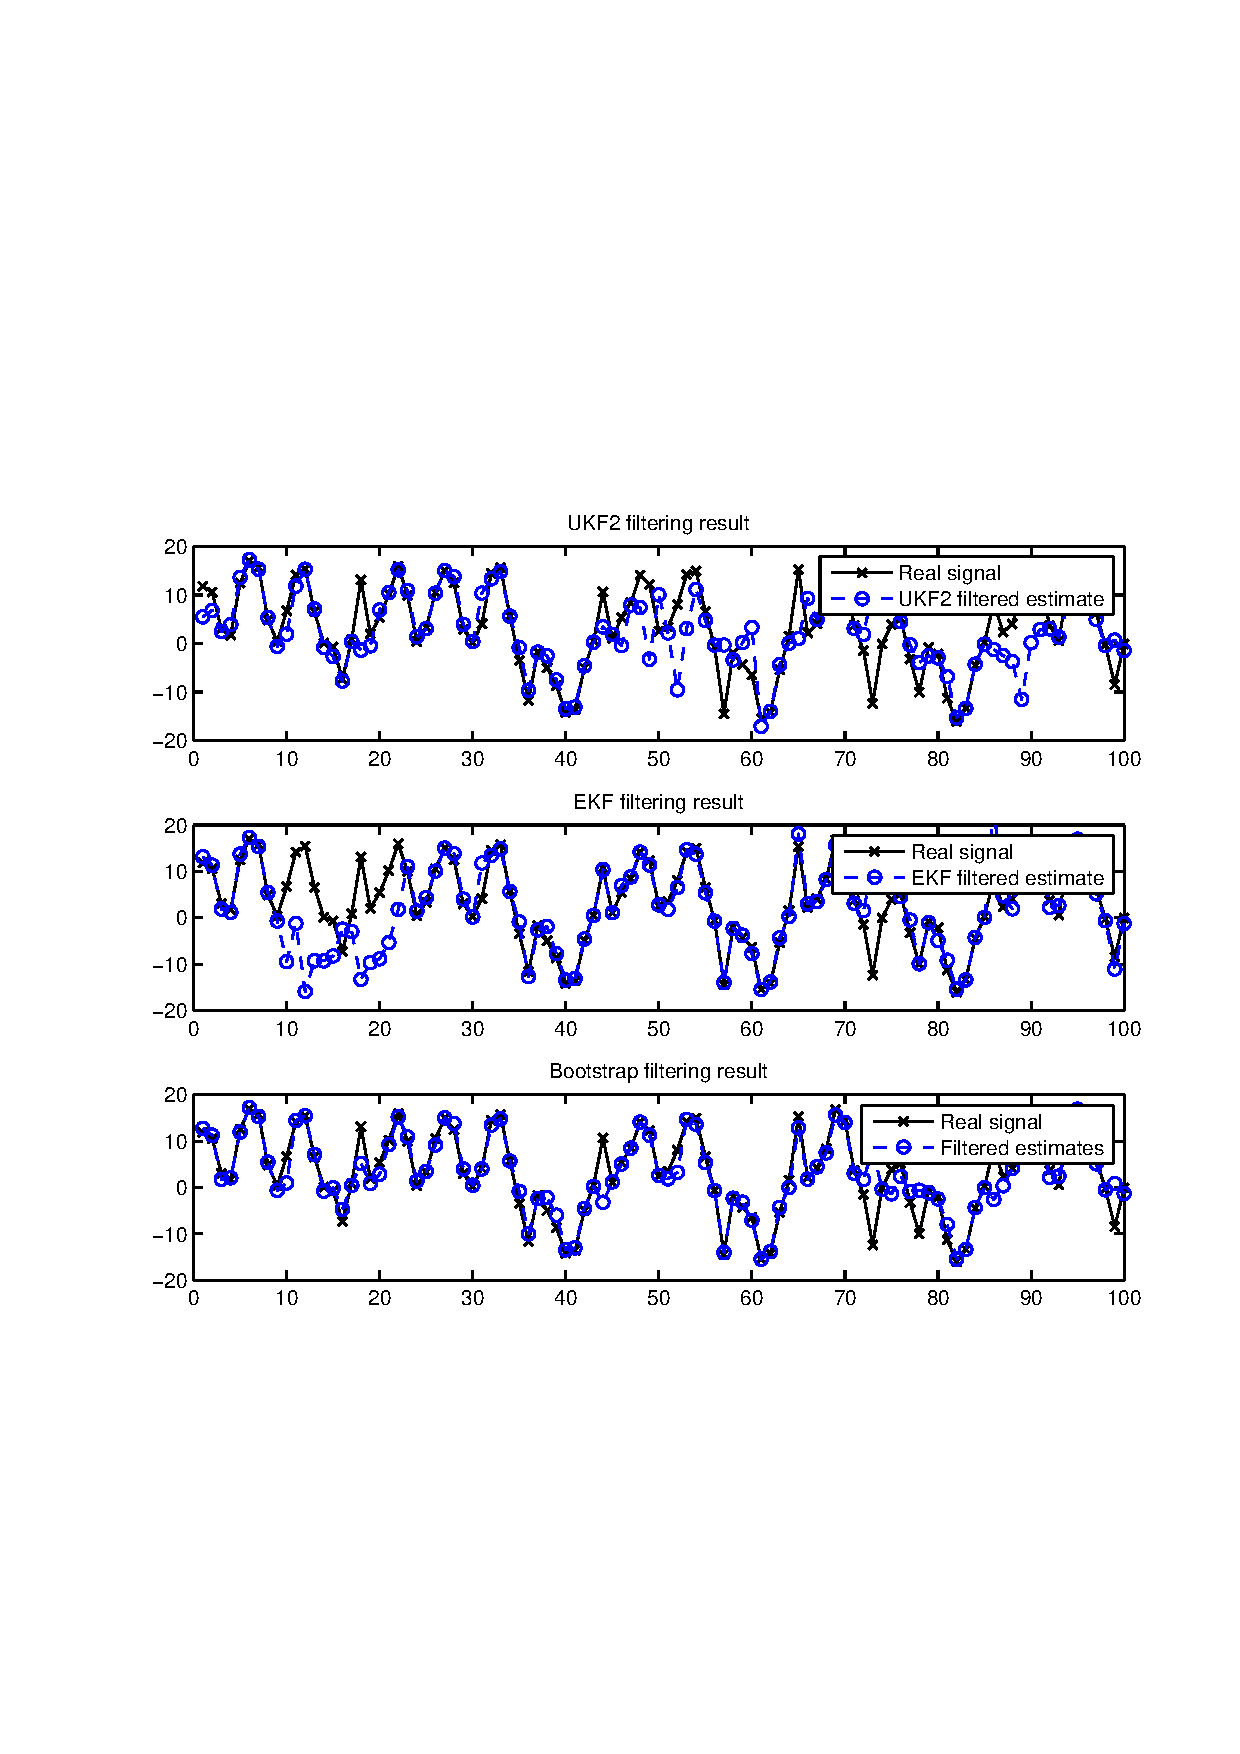
\includegraphics[width=11cm]{pics/ungm_states}
\caption{First 100 samples of filtering results of EKF, augmented form
UKF and bootstrap filter for UNGM-model.}
\label{fig:ungm_states}
\end{center}
\end{figure}

In figure \ref{fig:ungm_c_errors} we have plotted the absolute errors
and $3\sigma$ confidence intervals of the previous figures filtering
results. It can be seen that the EKF is overoptimistic in many cases
while UKF and boostrap filter are better at telling when their results
are unreliable. Also the lower error of bootstrap filter can be seen
from the figure. The bimodality is also easy to notice on those
samples, which were mentioned above.

\begin{figure}
\begin{center}
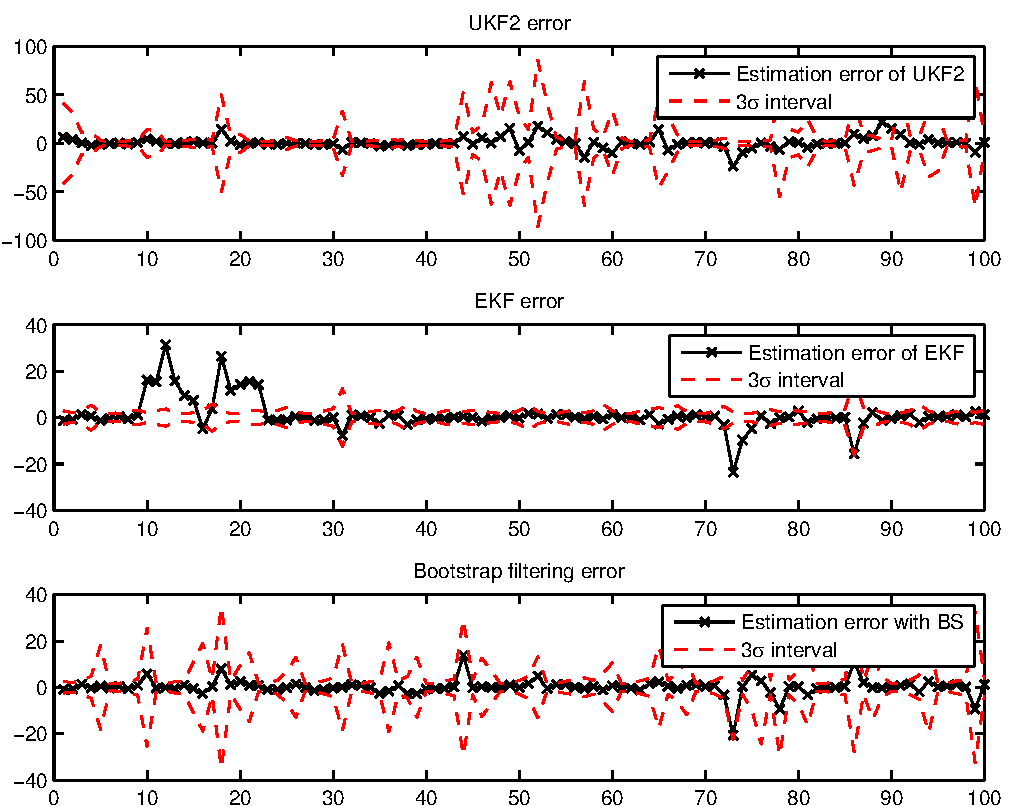
\includegraphics[width=11cm]{pics/ungm_c_errors}
\caption{Absolute errors of and $3\sigma$ confidence intervals of EKF,
augmented form UKF and bootstrap in 100 first samples.}
\label{fig:ungm_c_errors}
\end{center}
\end{figure}

The make a comparison between nonaugmented and augmented UKF we have
plotted 100 first samples of their filtering results in figure
\ref{fig:ungm_ukf_comp}. Results are very surprising (although same as
in \citet{Wu+Hu+Wu+Hu:2005}). The reason why nonaugmented UKF gave so bad
results is not clear. However, the better performance of augmented
form UKF can be explained by the fact, that the process noise is taken
into account more effectively when the sigma points are propagated
through nonlinearity. In this case it seems to be very crucial, as the
model is highly nonlinear and multi-modal.

\begin{figure}
\begin{center}
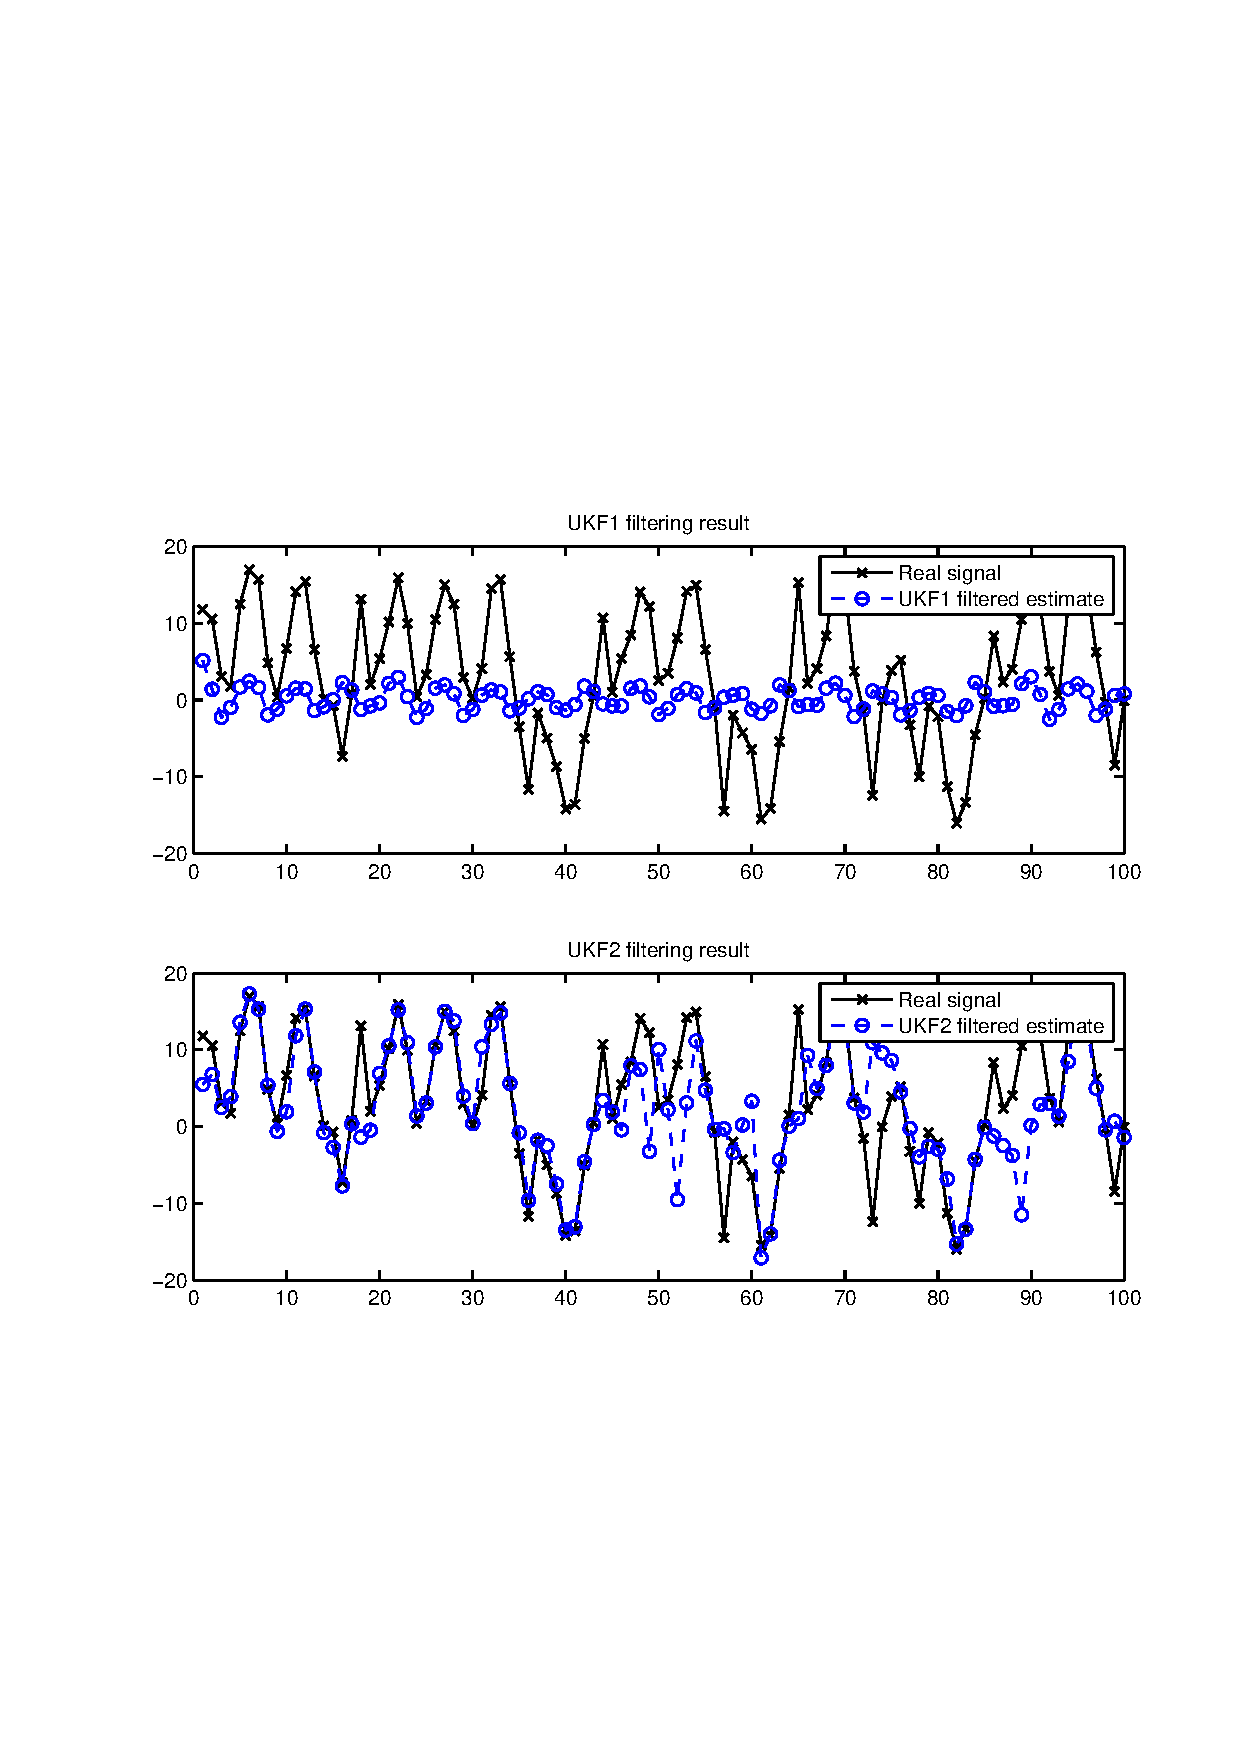
\includegraphics[width=11cm]{pics/ungm_ukf_comp}
\caption{Filtering results of nonaugmented UKF (UKF1) and augmented
UKF (UKF2) of 100 first samples.}
\label{fig:ungm_ukf_comp}
\end{center}
\end{figure}

Lastly in figure \ref{fig:ungm_mse} we have plotted the mean square
errors of each tested methods of 100 Monte Carlo runs. Average of
those errors are listed in table \ref{table:ungm_errors}. Here is a
discussion for the results:
%
\begin{itemize}
\item It is surprising that the nonaugmented UKF seems to be better
than EKF, while in above figures we have shown, that the nonaugmented
UKF gives very bad results. Reason for this is simple: the variance of
the actual signal is approximately 100, which means that by simply
guessing zero we get better performance than with EKF, on average. The
estimates of nonaugmented UKF didn't variate much on average, so they
were better than those of EKF, which on the other hand variated
greatly and gave huge errors in some cases. Because of this neither of
the methods should be used for this problem, but if one has to choose
between the two, that would be EKF, because in some cases it still
gave (more or less) right answers, whereas UKF were practically always
wrong.
\item The second order EKF were also tested, but that diverged almost
instantly, so it were left out from comparison.
\item Augmented form UKF gave clearly the best performance from the
tested Kalman filters. As discussed above, this is most likely due to
the fact that the process noise terms are propagated through the
nonlinearity, and hence odd-order moment information is used to obtain
more accurate estimates. The usage of RTS smoother seemed to improve
the estimates in general, but oddly in some cases it made the
estimates worse. This is most likely due to the multi-modality of the
filtering problem.
\item The Gauss--Hermite method performed rather well in both filtering and
smoothing. This was mostly due to the degree of approximation as the
rule entailed 10 sigma points.
\item The cubature Kalman filter gave results close to the UKF variants,
which is to no surprise as the filter uses similar sigma points.
\item Bootstrap filtering solution was clearly superior over all other
tested methods. The results had been even better, if greater amount of
particles had been used.
\end{itemize}

The reason why Kalman filters didn't work that well in this case is
because Gaussian approximations do not in general apply well for
multi-modal cases. Thus, a particle filtering solution should be
preferred over Kalman filters in such cases. However, usually the
particle filters need a fairly large amount of particles to be
effective, so they are generally more demanding in terms of
computational power than Kalman filters, which can be a limiting
factor in real world applications. The errors, even with bootstrap
filter, were also relatively large, so one must be careful when using
the estimates in, for example, making financial decisions. In practice
this means that one has to monitor the filter's covariance estimate,
and trust the state estimates and predictions only when the covariance
estimates are low enough, but even then there is a change, that the
filter's estimate is completely wrong.


\begin{figure}
\begin{center}
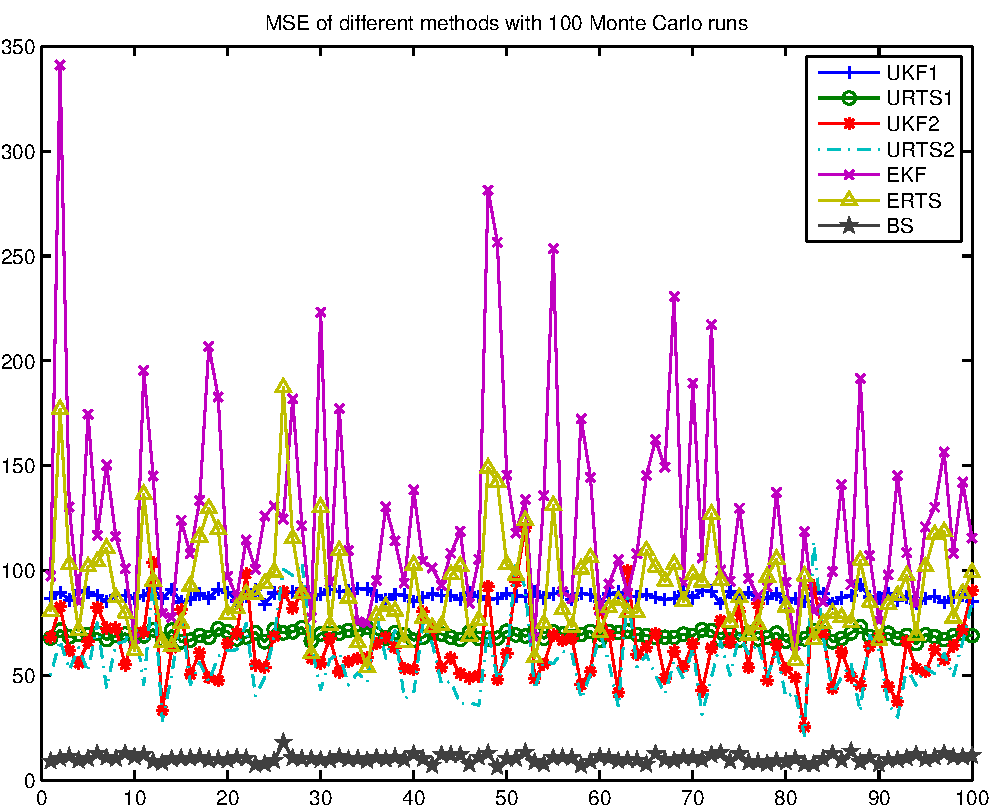
\includegraphics[width=11cm]{pics/ungm_mse}
\caption{MSEs of different methods in 100 Monte Carlo runs.}
\label{fig:ungm_mse}
\end{center}
\end{figure}

\begin{table}
\begin{center}
\begin{tabular}{|l|l|} \hline {\it Method}&{\it MSE[$x$]}\\ \hline
UKF1 & 87.9 \\ URTS1& 69.09 \\ UKF2 & 63.7 \\ URTS2 & 57.7 \\ EKF &
125.9 \\ ERTS & 92.2 \\ BS & 10.2 \\
GHKF & 40.9 \\
GHRTS & 31.6 \\
CKF & 72.3 \\
CRTS & 71.4 \\
 \hline
\end{tabular}
\caption{MSEs of estimating the UNGM model over 100 Monte Carlo
simulations.}
\label{table:ungm_errors}
\end{center}
\end{table}
 



\clearpage
\section{Demonstration: Bearings Only Tracking}

Next we review a classical filtering application \citep[see, e.g.,][]{Bar-Shalom+Li+Kirubarajan:2001}, in which we track a moving object with
sensors, which measure only the bearings (or angles) of the object
with respect positions of the sensors. There is a one moving target in
the scene and two angular sensors for tracking it. Solving this
problem is important, because often more general multiple target
tracking problems can be partitioned into sub-problems, in which
single targets are tracked separately at a time \citep{Sarkka+Vehtari+Lampinen:2007}.

The state of the target at time step $k$ consists of the position in
two dimensional cartesian coordinates $x_k$ and $y_k$ and the velocity
toward those coordinate axes, $\dot{x}_k$ and $\dot{y}_k$. Thus, the
state vector can be expressed as
%
\begin{equation}
%
\vec{x}_k =
\begin{pmatrix} x_k & y_k & \dot{x}_k & \dot{y}_k
\end{pmatrix}^T.
%
\end{equation}
%
The dynamics of the target is modelled as a linear, discretized Wiener
velocity model \citep{Bar-Shalom+Li+Kirubarajan:2001}
%
\begin{equation}
%
\vec{x}_k = \begin{pmatrix} 1 & 0 & \dt & 0 \\ 0 & 1 & 0 & \dt \\ 0 &
0 & 1 & 0 \\ 0 & 0 & 0 & 1
\end{pmatrix} % *
\begin{pmatrix} x_{k-1} \\ y_{k-1} \\ \dot{x}_{k-1} \\ \dot{y}_{k-1}
\end{pmatrix} + \vec{q}_{k-1},
%
\end{equation}
% 
where $\vec{q}_{k-1}$ is Gaussian process noise with zero mean and
covariance
%
\begin{equation}
\begin{split} E[\vec{q}_{k-1}\vec{q}^T_{k-1}] = \begin{pmatrix}
\frac{1}{3}\dt^3 & 0 & \frac{1}{2}\dt^2 & 0 \\ 0 & \frac{1}{3}\dt^3 &
0 & \frac{1}{2}\dt^2 \\ \frac{1}{2}\dt^2 & 0 & \dt & 0 \\ 0 &
\frac{1}{2}\dt^2 & 0 & \dt
\end{pmatrix} \\
\end{split}q,
\end{equation}
%
where $q$ is the spectral density of the noise, which is set to
$q=0.1$ in the simulations. The measurement model for sensor $i$ is
defined as
%
\begin{equation}
%
\theta^i_k = \arctan \left( \frac{y_k - s^i_y}{x_k - s^i_x}\right) +
r^i_k,
%
\end{equation}
%
where $(s^i_x,s^i_y)$ is the position of sensor $i$ and $r^i_k \sim
N(0,\sigma^2)$, with $\sigma = 0.05$ radians. In figure
\ref{fig:bot_measurements} we have plotted a one realization of
measurements in radians obtained from both sensors. The sensors are
placed to $(s^1_x,s^1_y) = (-1,-2)$ and $(s^2_x,s^2_y) = (1,1)$.
%
\begin{figure}
\begin{center}
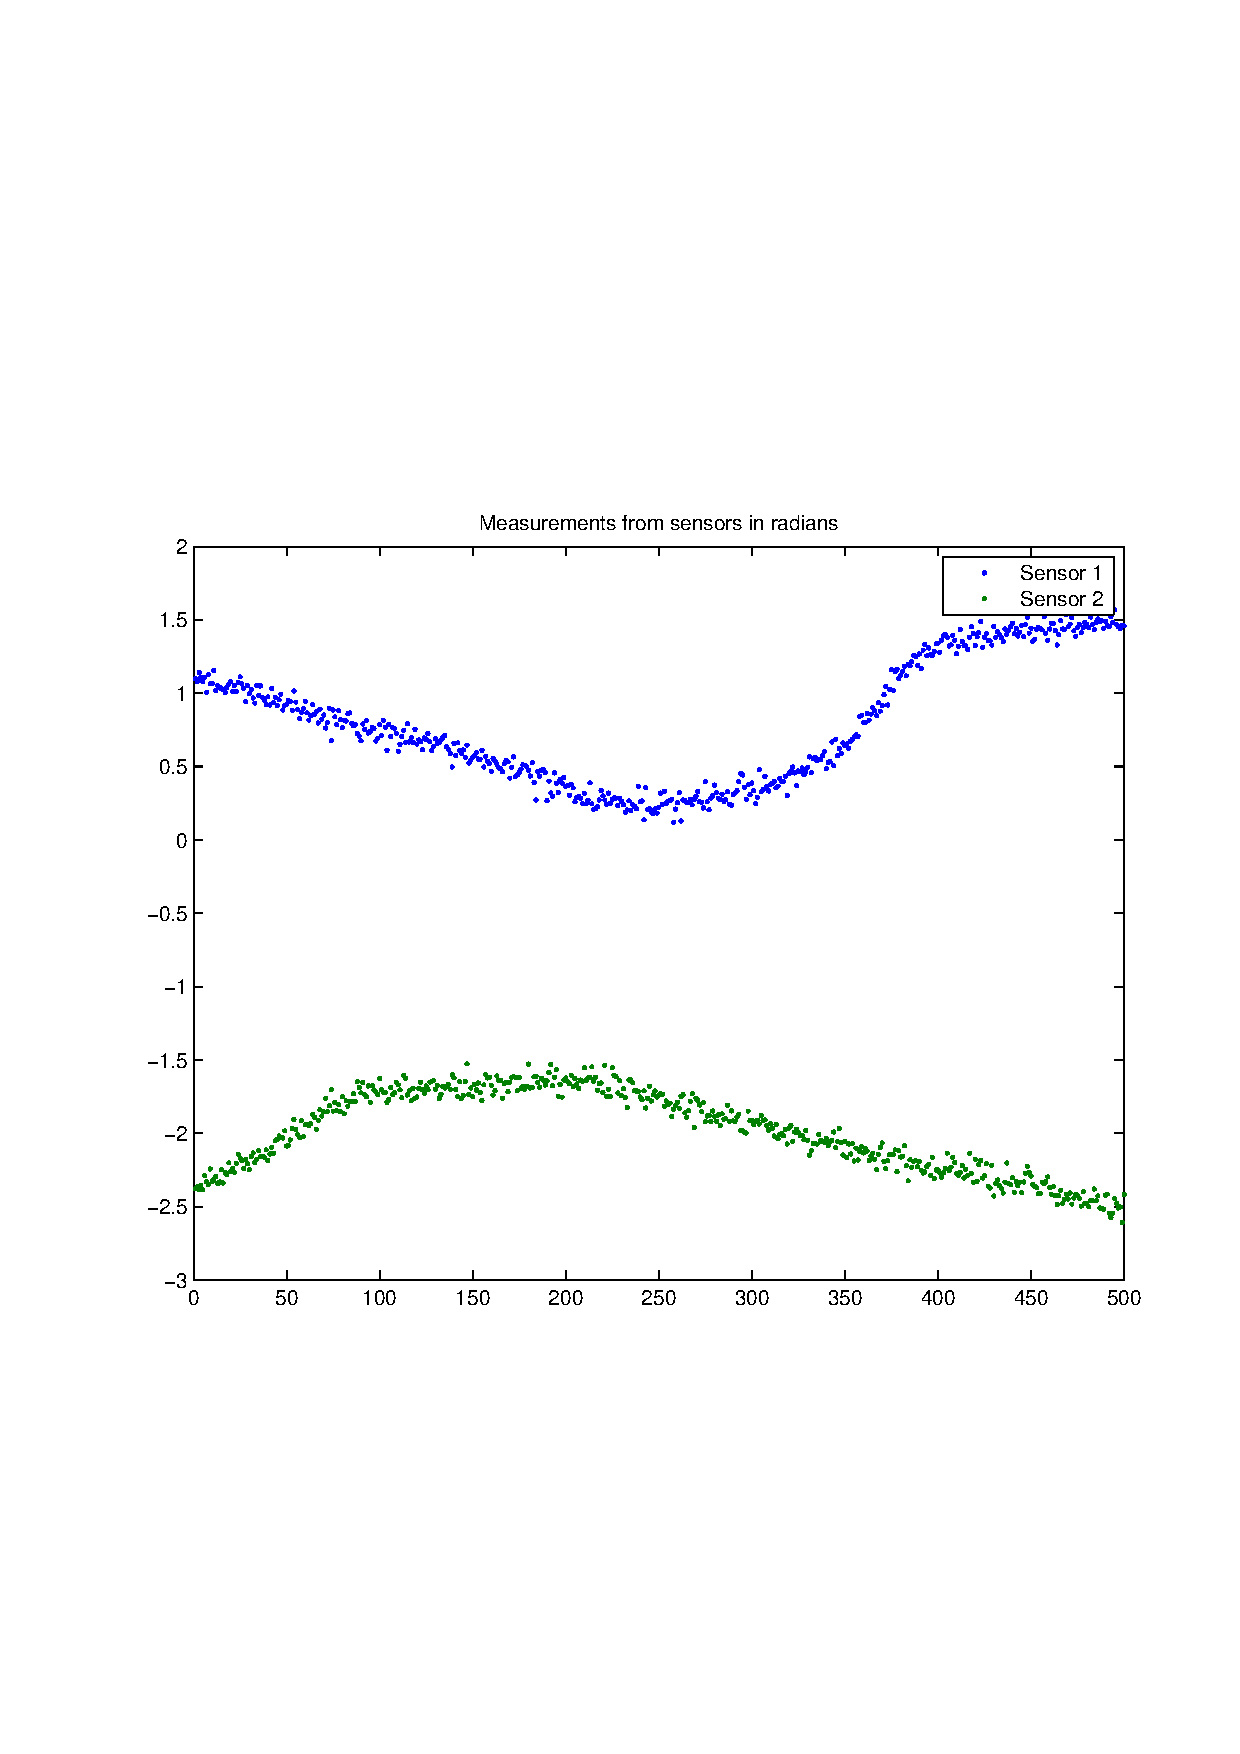
\includegraphics[width=11cm]{pics/bot_demo_measurements}
\caption{Measurements from sensors (in radians) in bearings only
tracking problem .}
\label{fig:bot_measurements}
\end{center}
\end{figure}

The derivatives of the measurement model, which are needed by EKF, can
be computed as
%
\begin{equation}
\begin{split} \frac{\partial \vec{h}^i(\vec{x}_k)}{\partial x_k} & =
\frac{-(y_k-s^i_y)}{(x_k-s^i_x)^2+(y_k-s^i_y)^2} \\ \frac{\partial
\vec{h}^i(\vec{x}_k)}{\partial y_k} & =
\frac{(x_k-s^i_x)}{(x_k-s^i_x)^2+(y_k-s^i_y)^2} \\ \frac{\partial
\vec{h}^i(\vec{x}_k)}{\partial \dot{x}_k} & = 0 \\ \frac{\partial
\vec{h}^i(\vec{x}_k)}{\partial \dot{y}_k} & = 0 , i = 1,2.
\end{split}
\label{eq:bot_dx}
\end{equation}
%
With these the Jacobian can written as
%
\begin{equation} \mat{H}_\vec{x}(\vec{x}_k,k) = \begin{pmatrix}
\frac{(x_k-s^1_x)}{(x_k-s^1_x)^2+(y_k-s^1_y)^2} &
\frac{-(y_k-s^1_y)}{(x_k-s^1_x)^2+(y_k-s^1_y)^2} & 0 & 0 \\
\frac{(x_k-s^2_x)}{(x_k-s^2_x)^2+(y_k-s^2_y)^2} &
\frac{-(y_k-s^2_y)}{(x_k-s^2_x)^2+(y_k-s^2_y)^2} & 0 & 0
\end{pmatrix}.
\end{equation}
%
The non-zero second order derivatives of the measurement function are
also relatively easy to compute in this model:
%
\begin{equation}
\begin{split} \frac{\partial^2 \vec{h}^i(\vec{x}_k)}{\partial x_k
\partial x_k} & =
\frac{-2(x_k-s^i_x)}{((x_k-s^i_x)^2+(y_k-s^i_y)^2)^2} \\
\frac{\partial^2 \vec{h}^i(\vec{x}_k)}{\partial x_k \partial y_k} & =
\frac{(y_k-s^i_y)^2-(x_k-s^i_x)^2}{((x_k-s^i_x)^2+(y_k-s^i_y)^2)^2} \\
\frac{\partial^2 \vec{h}^i(\vec{x}_k)}{\partial y_k \partial y_k} & =
\frac{-2(y_k-s^i_y)}{((x_k-s^i_x)^2+(y_k-s^i_y)^2)^2}.
\end{split}
\end{equation}
%
Thus, the Hessian matrices can be written as
%
\begin{equation} \mat{H}^i_\vec{xx}(\vec{x}_k,k) = \begin{pmatrix}
\frac{-2(x_k-s^i_x)}{((x_k-s^i_x)^2+(y_k-s^i_y)^2)^2} &
\frac{(y_k-s^i_y)^2-(x_k-s^i_x)^2}{((x_k-s^i_x)^2+(y_k-s^i_y)^2)^2} &
0 & 0 \\
\frac{(y_k-s^i_y)^2-(x_k-s^i_x)^2}{((x_k-s^i_x)^2+(y_k-s^i_y)^2)^2} &
\frac{-2(y_k-s^i_y)}{((x_k-s^i_x)^2+(y_k-s^i_y)^2)^2} & 0 & 0 \\ 0 & 0
& 0 & 0 \\ 0 & 0 & 0 & 0
\end{pmatrix}, i=1,2.
\end{equation}
%
We do not list the program code for the measurement function and it's
derivatives here as they are straightforward to implement, if the
previous examples have been read.

The target starts with state $\vec{x}_0 = \begin{pmatrix} 0 & 0 & 1 &
0
\end{pmatrix}$, and in the estimation we set the prior distribution
for the state to $\vec{x}_0 \sim N(\vec{0},\mat{P}_0)$, where
%
\begin{equation}
%
\mat{P}_0 = \begin{pmatrix} 0.1 & 0 & 0 & 0\\ 0 & 0.1 & 0 & 0\\ 0 & 0
& 10 & 0\\ 0 & 0 & 0 & 10
\end{pmatrix},
%
\end{equation}
%
which basically means that we are fairly certain about the target's
origin, but very uncertain about the velocity. In the simulations we
also give the target an slightly randomized acceleration, so that it
achieves a curved trajectory, which is approximately the same in
different simulations. The trajectory and estimates of it can be seen
in figures \ref{fig:bot_ekf1}, \ref{fig:bot_ekf2} and
\ref{fig:bot_ukf}. As can be seen from the figures EKF1 and UKF give
almost identical results while the estimates of EKF2 are clearly
worse. Especially in the beginning of the trajectory EKF2 has great
difficulties in getting on the right track, which is due to the
relatively big uncertainty in the starting velocity. After that the
estimates are fairly similar.

In table \ref{table:bot_rmse} we have listed the root mean square
errors (mean of position errors) of all tested methods (same as in
random sine signal example on page \pageref{page:sine_rmse} with the
addition of UTF) over 1000 Monte Carlo runs. The numbers prove the
previous observations, that the EKF1 and UKF give almost identical
performances. Same observations apply also to smoothers. Had the prior
distribution for the starting velocity been more accurate the
performance difference between EKF2 and other methods would have been
smaller, but still noticeable.

These observations also hold for the cubature methods. The Gauss--Hermite
Kalman filter and cubature Kalman filter give practically identical 
results as the unscented filter.

\begin{table}
\begin{center}
\begin{tabular}{|l|l|} \hline {\it Method}&{\it RMSE } \\ \hline 
  EKF1  & 0.114 \\ 
  ERTS1 & 0.054 \\ 
  ETF1  & 0.054 \\ 
  EKF2  & 0.202 \\ 
  ERTS2 & 0.074 \\ 
  ETF2  & 0.063 \\ 
  UKF   & 0.113 \\ 
  URTS  & 0.055 \\ 
  UTF   & 0.055 \\
  GHKF  & 0.107 \\
  GHRTS & 0.053 \\
  CKF   & 0.108 \\
  CRTS  & 0.053 \\
\hline
\end{tabular}
\caption{RMSEs of estimating the position in Bearings Only Tracking
problem over 1000 Monte Carlo runs. The Gauss--Hermite rule is of degree 3.}
\label{table:bot_rmse}
\end{center}
\end{table}

%
\begin{figure}
\begin{center}
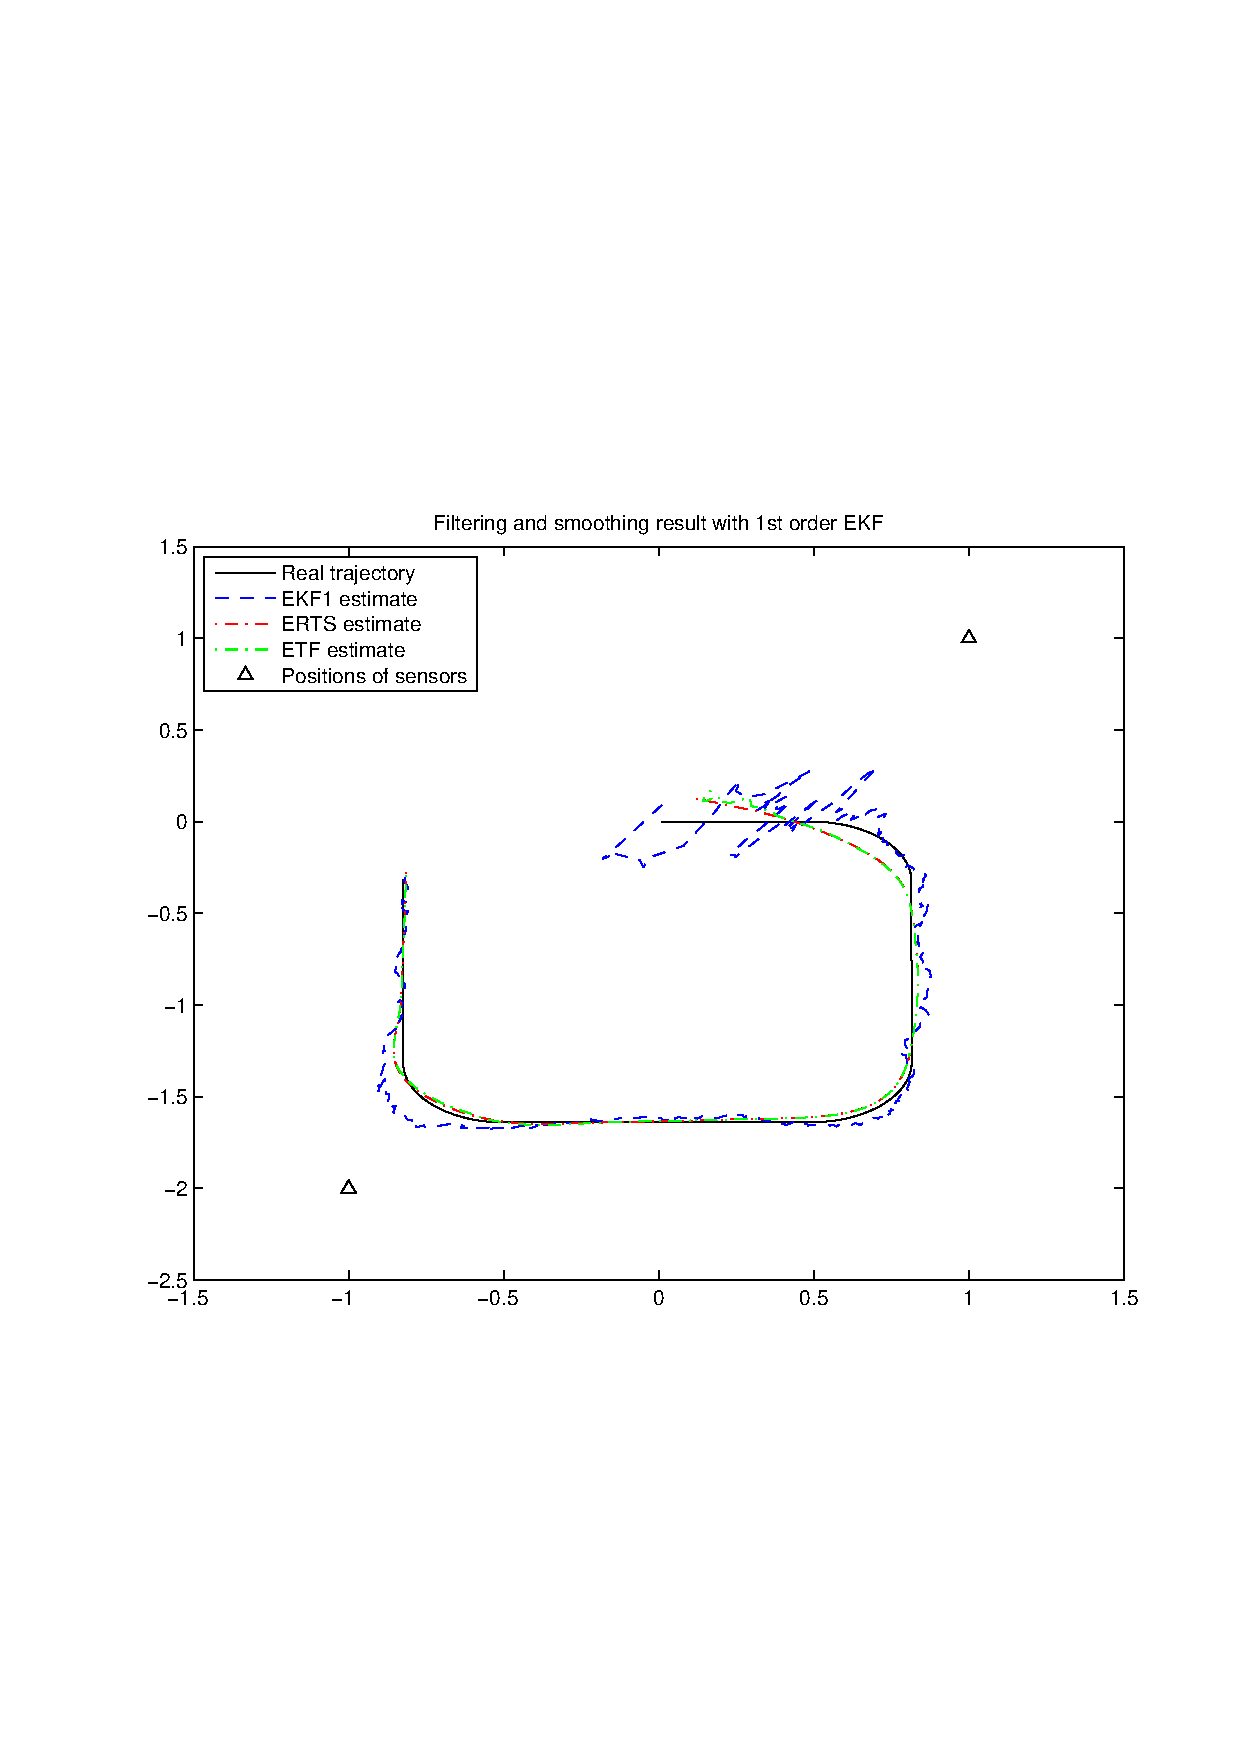
\includegraphics[width=11cm]{pics/bot_demo_ekf1}
\caption{Filtering and smoothing results of first order EKF.}
\label{fig:bot_ekf1}
\end{center}
\end{figure}

%
\begin{figure}
\begin{center}
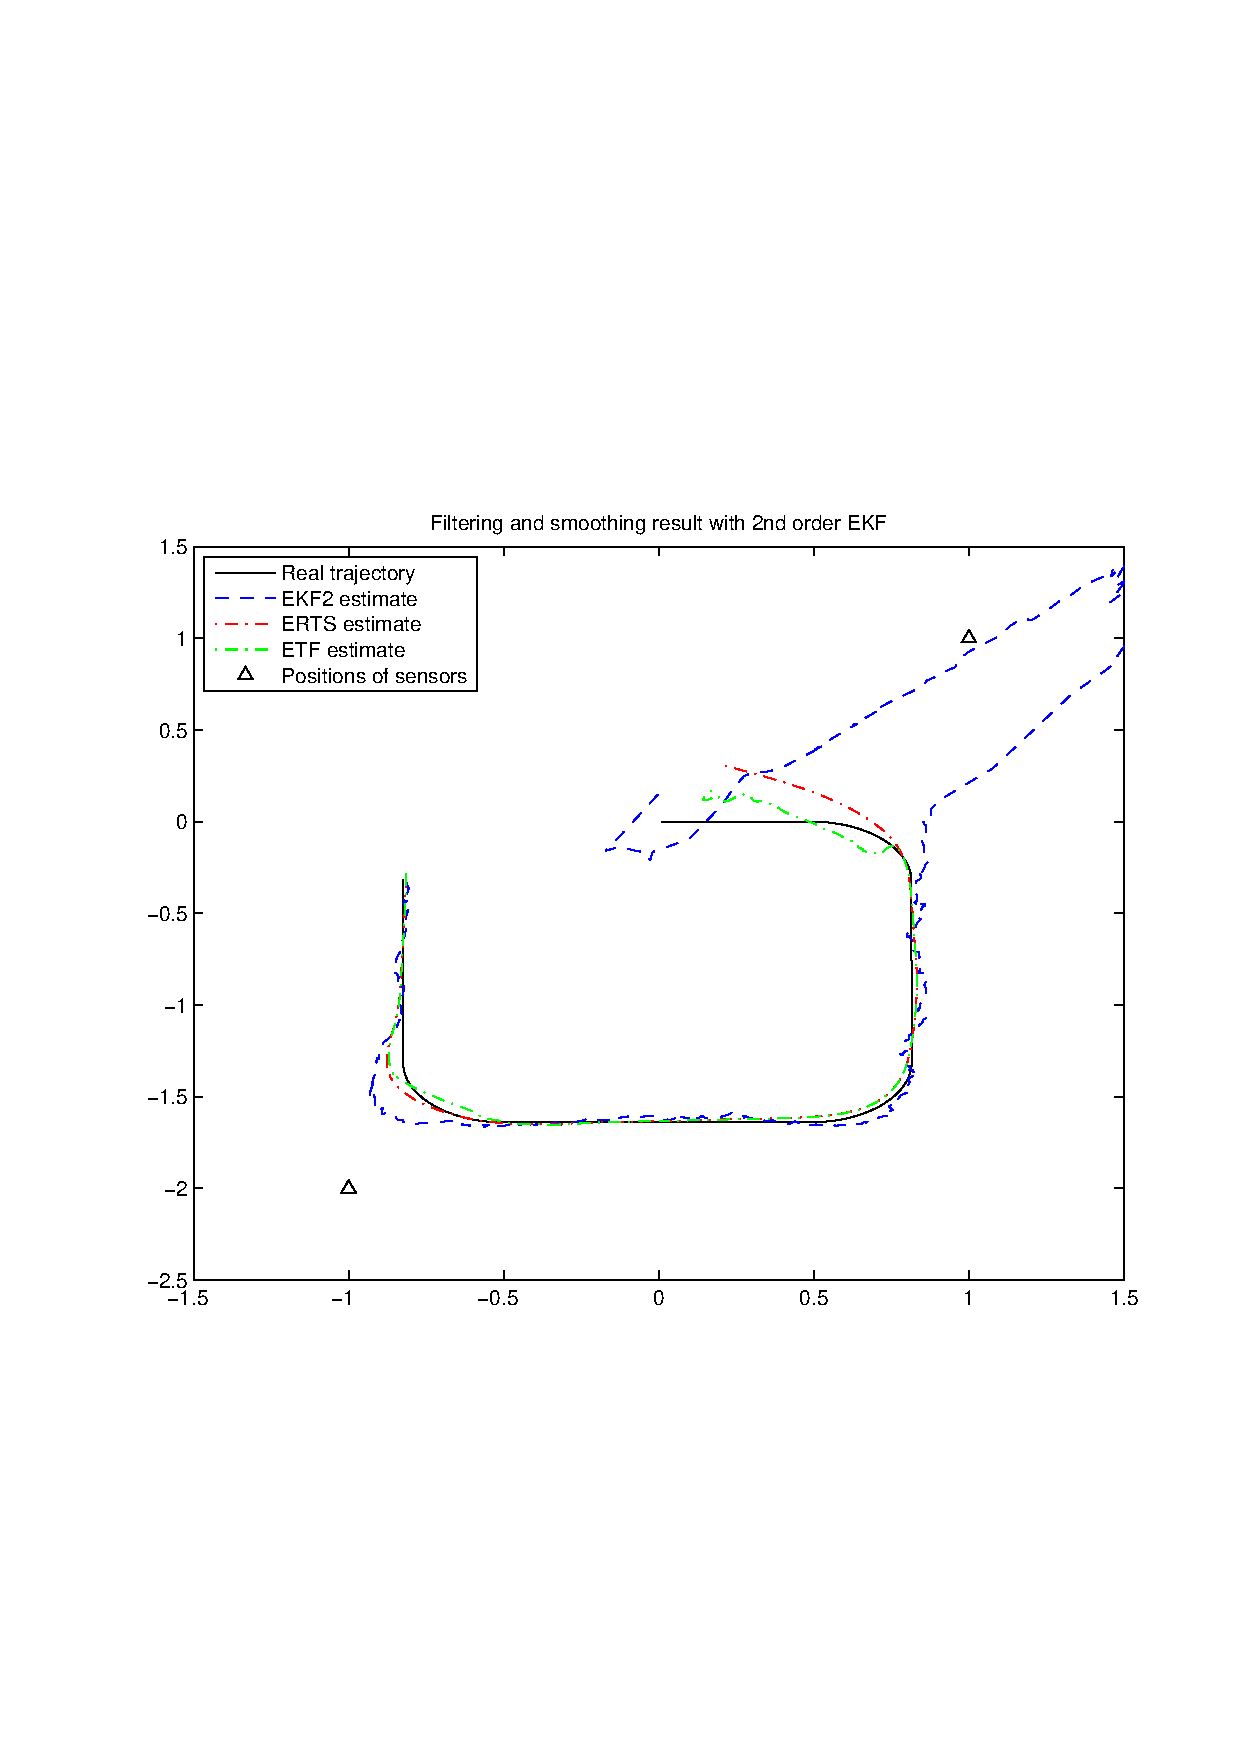
\includegraphics[width=11cm]{pics/bot_demo_ekf2}
\caption{Filtering and smoothing results of second order EKF.}
\label{fig:bot_ekf2}
\end{center}
\end{figure}

\begin{figure}
\begin{center}
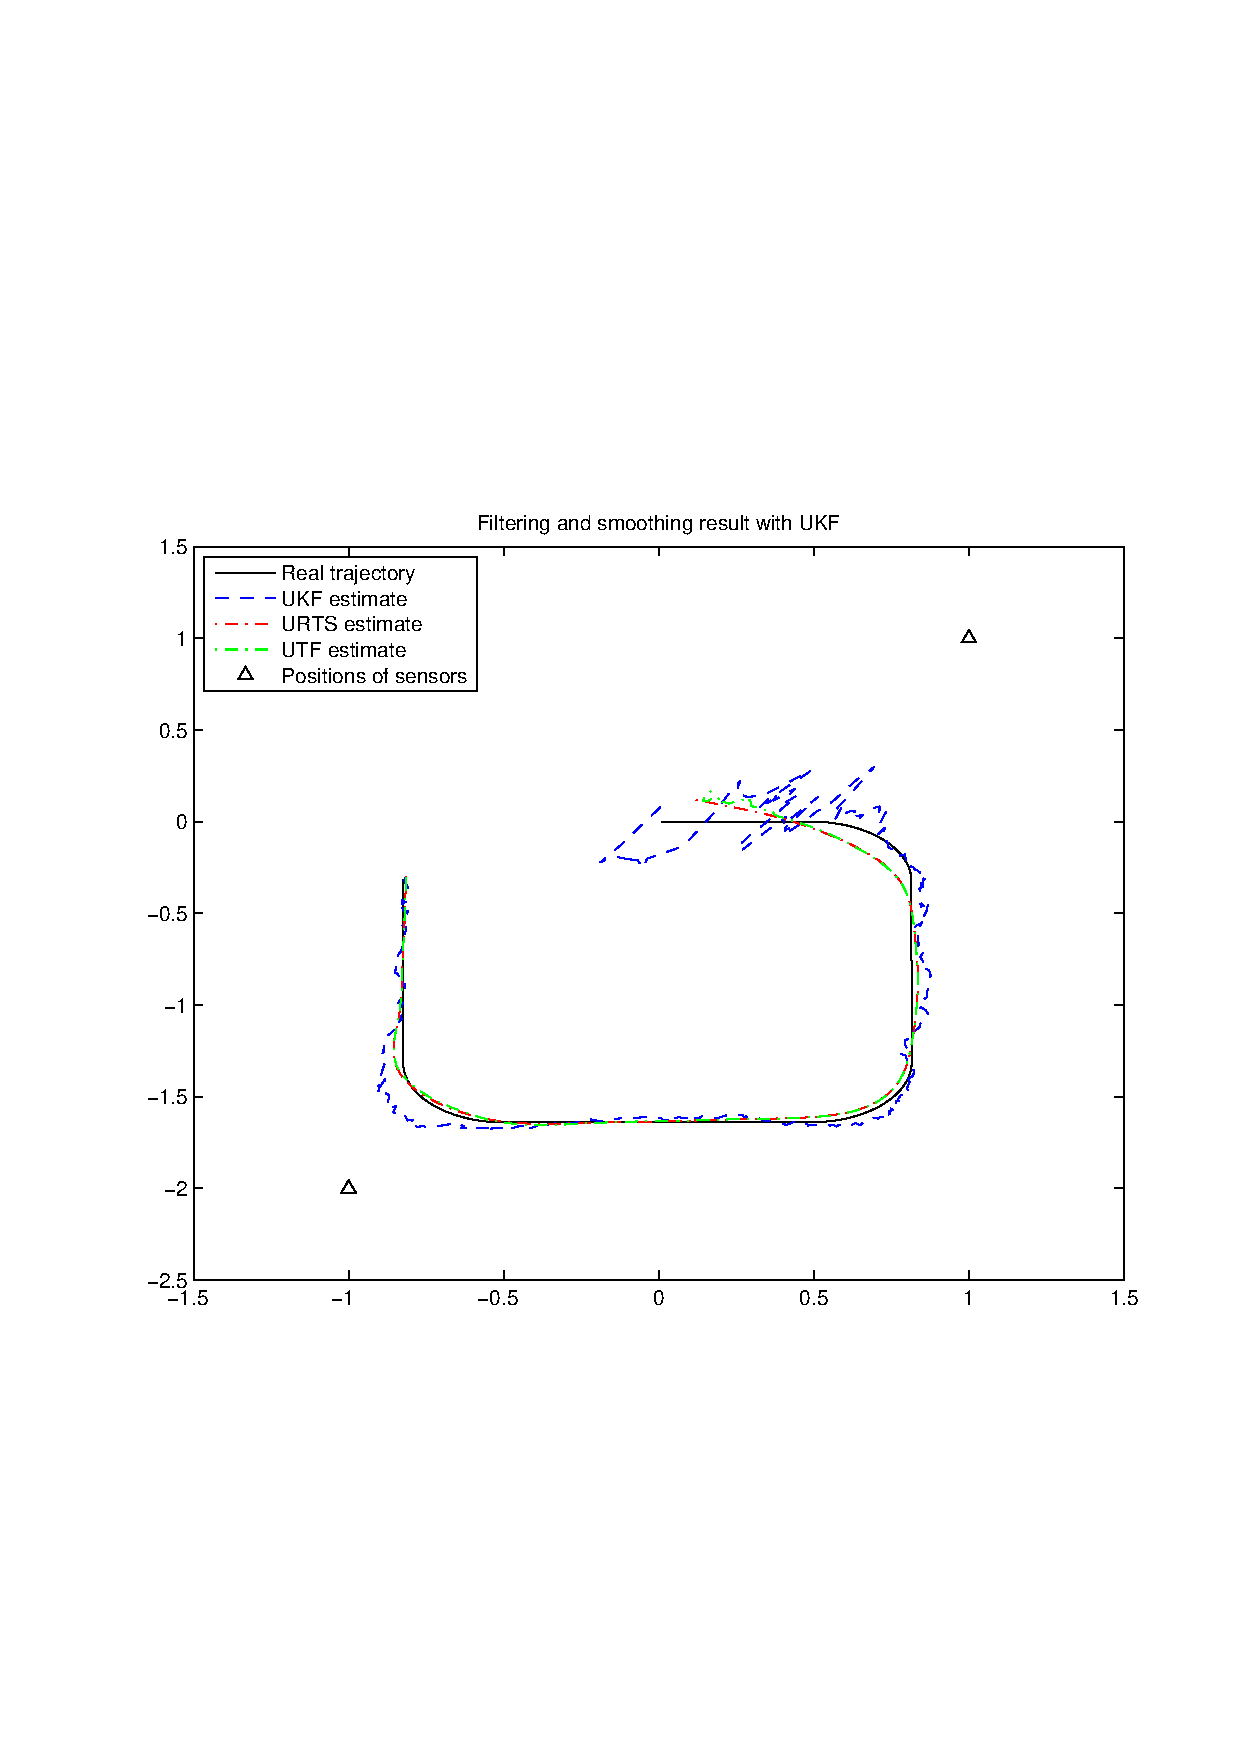
\includegraphics[width=11cm]{pics/bot_demo_ukf}
\caption{Filtering and smoothing results of UKF}
\label{fig:bot_ukf}
\end{center}
\end{figure}












\clearpage
\section{Demonstration: Reentry Vehicle Tracking}

Next we review a challenging filtering problem, which was used in
\citet{Julier+Uhlmann:2004} to demonstrate the performance of
UKF. Later they released few corrections to the model specifications
and simulation parameters in \citet{Julier+Uhlmann:2004b}.

This example conserns a reentry tracking problem, where radar is used
for tracking a space vehicle, which enters the atmosphere at high
altitude and very high speed. Figure \ref{fig:reentry_traj} shows a
sample trajectory of the vehicle with respect to earth and radar. The
dynamics of the vehicle are affected with three kinds of forces:
aerodynamic drag, which is a function of vehicle speed and has highly
nonlinear variations in altitude. The second type of force is gravity,
which causes the vehicle to accelerate toward the center of the
earth. The third type of forces are random buffeting terms. The state
space in this model consists of vehicles position ($x_1$ and $x_2$),
its velocity ($x_3$ and $x_4$) and a parameter of its aerodynamic
properties ($x_5$).  The dynamics in continuous case are defined as
\citep{Julier+Uhlmann:2004}
%
\begin{equation}
\begin{split}
%
\dot{x}_1(t) & = x_3(t) \\ \dot{x}_2(t) & = x_4(t) \\ \dot{x}_3(t) & =
D(t)x_3(t) + G(t)x_1(t) + v_1(t) \\ \dot{x}_4(t) & = D(t)x_4(t) +
G(t)x_2(t) + v_2(t) \\ \dot{x}_5(t) & = v_3(t),
%
\end{split}
\end{equation}
%
where $\vec{w}(t)$ is the process noise vector, $D(t)$ the
drag-related force and $G(t)$ the gravity-related force.  The force
terms are given by
%
\begin{equation}
\begin{split}
%
D(k) & = \beta(t) \exp \left\{ \frac{[R_0 - R(t)]}{H_0}\right\} V(t)
\\ G(t) & = -\frac{Gm_0}{R^3(t)} \\ \beta (t) & = \beta_0 \exp x_5(t),
%
\end{split}
\end{equation}
%
where $R(t) = \sqrt{x_1^2(t) + x_2^2(t)}$ is the vehicle's distance
from the center of the earth and $V(t) = \sqrt{x_3^2(t) + x_4^2(t)}$
is the speed of the vehicle.  The constants in previous definition
were set to
%
\begin{equation}
\begin{split}
%
\beta_0 & = -0.59783 \\ H_0 & = 13.406 \\ Gm_0 & = 3.9860 \times 10^5
\\ R_0 & = 6374.
%
\end{split}
\end{equation}
%
To keep the implementation simple the continuous-time dynamic
equations were discretized using a simple Euler integration scheme, to
give
%
\begin{equation}
\begin{split}
%
x_1(k+1) & = x_1(k) + \dt x_3(k) \\ x_2(k+1) & = x_2(k) + \dt x_4(k)
\\ x_3(k+1) & = x_3(k) + \dt (D(k)x_3(k) + G(k)x_1(k)) + w_1(k) \\
x_4(k+1) & = x_4(k) + \dt (D(k)x_4(k) + G(k)x_2(k)) + w_2(k) \\
x_5(k+1) & = x_5(k) + w_3(k),
%
\end{split}
\end{equation}
%
where the step size between time steps was set to $\dt = 0.1s$. Note
that this might be too simple approach in real world applications due
to high nonlinearities in the dynamics, so more advanced integration
scheme (such as Runge-Kutta) might be more preferable. The discrete
process noise covariance in the simulations was set to
%
\begin{equation}
%
Q(k) = \begin{pmatrix} 2.4064 \times 10^{-5} & 0 & 0 \\ 0 & 2.4064
\times 10^{-5} & 0 \\ 0 & 0 & 10^{-6}
\end{pmatrix}.
%
\end{equation}
%
The lower right element in the covariance was initially in \citet{Julier+Uhlmann:2004} set to zero, but later in \citet{Julier+Uhlmann:2004b}
changed to $10^{-6}$ to increase filter stability.


The non-zero derivatives of the discretized dynamic equations with
respect to state variables are straightforward (although rather
technical) to compute:
%
\begin{equation}
\begin{split}
%
\frac{\partial x_1(k+1)}{\partial x_1(k)} & = 1 \\ \frac{\partial
x_1(k+1)}{\partial x_3(k)} & = \dt \\ \frac{\partial
x_2(k+1)}{\partial x_2(k)} & = 1 \\ \frac{\partial x_2(k+1)}{\partial
x_4(k)} & = \dt \\
%
\frac{\partial x_3(k+1)}{\partial x_1(k)} & = \dt * (\frac{\partial
D(k)}{\partial x_1(k)} x_3(k) + \frac{\partial G(k)}{\partial x_1(k)}
x_1(k) + G(k)) \\ \frac{\partial x_3(k+1)}{\partial x_2(k)} & = \dt *
(\frac{\partial D(k)}{\partial x_2(k)} x_3(k) + \frac{\partial
G(k)}{\partial x_2(k)} x_1(k)) \\ \frac{\partial x_3(k+1)}{\partial
x_3(k)} & = \dt * (\frac{\partial D(k)}{\partial x_3(k)} x_3(k) +
D(k)) + 1 \\ \frac{\partial x_3(k+1)}{\partial x_4(k)} & = \dt *
(\frac{\partial D(k)}{\partial x_4(k)} x_3(k)) \\ \frac{\partial
x_3(k+1)}{\partial x_4(k)} & = \dt * (\frac{\partial D(k)}{\partial
x_5(k)} x_3(k)) \\
%
\frac{\partial x_4(k+1)}{\partial x_1(k)} & = \dt * (\frac{\partial
D(k)}{\partial x_1(k)} x_4(k) + \frac{\partial G(k)}{\partial x_1(k)}
x_2(k)) \\ \frac{\partial x_4(k+1)}{\partial x_2(k)} & = \dt *
(\frac{\partial D(k)}{\partial x_2(k)} x_4(k) + \frac{\partial
G(k)}{\partial x_2(k)} x_2(k) + G(k)) \\ \frac{\partial
x_4(k+1)}{\partial x_3(k)} & = \dt * (\frac{\partial D(k)}{\partial
x_3(k)} x_4(k)) \\ \frac{\partial x_4(k+1)}{\partial x_4(k)} & = \dt *
(\frac{\partial D(k)}{\partial x_4(k)} x_4(k) + D(k)) + 1 \\
\frac{\partial x_4(k+1)}{\partial x_5(k)} & = \dt * (\frac{\partial
D(k)}{\partial x_5(k)} x_4(k)) \\ \frac{\partial x_5(k+1)}{\partial
x_5(k)} & = 1,
%
\end{split}
\end{equation}
%
where the (non-zero) derivatives of the force, position and velocity
related terms with respect to state variables can be computed as
%
\begin{equation}
\begin{split}
%
\frac{\partial R(k)}{\partial x_1(k)} & = x_1(k) \frac{1}{R(k)} \\
\frac{\partial R(k)}{\partial x_2(k)} & = x_2(k) \frac{1}{R(k)} \\
\frac{\partial V(k)}{\partial x_3(k)} & = x_3(k) \frac{1}{V(k)} \\
\frac{\partial V(k)}{\partial x_4(k)} & = x_4(k) \frac{1}{V(k)} \\
\frac{\partial \beta(k)}{\partial x_5(k)} & = \beta(k)\frac{1}{R(k)}
\\ \frac{\partial D(k)}{\partial x_1(k)} & = -\frac{\partial
R(k)}{\partial x_1(k)} \frac{1}{H_0} * D(k) \\ \frac{\partial
D(k)}{\partial x_2(k)} & = -\frac{\partial R(k)}{\partial x_2(k)}
\frac{1}{H_0} * D(k) \\ \frac{\partial D(k)}{\partial x_3(k)} & =
\beta(k) \exp \left\{ \frac{[R_0 - R(k)]}{H_0}\right\} \frac{\partial
V(k)}{\partial x_3} \\ \frac{\partial D(k)}{\partial x_4(k)} & =
\beta(k) \exp \left\{ \frac{[R_0 - R(k)]}{H_0}\right\} \frac{\partial
V(k)}{\partial x_4} \\ \frac{\partial D(k)}{\partial x_5(k)} & =
\frac{\partial \beta(k)}{x_5(k)} \exp \left\{ \frac{[R_0 -
R(k)]}{H_0}\right\} V(k) \\ \frac{\partial G(k)}{\partial x_1(k)} & =
\frac{3 Gm_0}{(R(k))^4} \frac{\partial R(k)}{\partial x_1(k)} \\
\frac{\partial G(k)}{\partial x_2(k)} & = \frac{3 Gm_0}{(R(k))^4}
\frac{\partial R(k)}{\partial x_2(k)}.
%
\end{split}
\end{equation}
%
The prior distribution for the state was set to multivariate Gaussian,
with mean and covariance (same as in \citet{Julier+Uhlmann:2004})
%
\begin{equation}
\begin{split}
%
\vec{m}_0 & = \begin{pmatrix} 6500.4 \\ 349.14 \\ -1.8093 \\ -6.7967
\\ 0 \\
\end{pmatrix} \\ \mat{P}_0 & = \begin{pmatrix} 10^{-6} & 0 & 0 & 0 & 0
\\ 0 & 10^{-6}& 0 & 0 & 0 \\ 0 & 0 & 10^{-6} & 0 & 0 \\ 0 & 0 & 0 &
10^{-6}& 0 \\ 0 & 0 & 0 & 0 & 1
\end{pmatrix}.
%
\end{split}
\end{equation}
%
In the simulations the initial state were drawn from multivariate
Gaussian with mean and covariance
%
\begin{equation}
\begin{split}
%
\vec{m}_0 & = \begin{pmatrix} 6500.4 \\ 349.14 \\ -1.8093 \\ -6.7967
\\ 0.6932 \\
\end{pmatrix} \\ \mat{P}_0 & = \begin{pmatrix} 10^{-6} & 0 & 0 & 0 & 0
\\ 0 & 10^{-6}& 0 & 0 & 0 \\ 0 & 0 & 10^{-6} & 0 & 0 \\ 0 & 0 & 0 &
10^{-6}& 0 \\ 0 & 0 & 0 & 0 & 0
\end{pmatrix},
%
\end{split}
\end{equation}
%
that is, vehicle's aerodynamic properties were not known precisely
beforehand.

The radar, which is located at $(s_x, s_y) = (R_0,0)$, is used to
measure the range $r_k$ and bearing $\theta_k$ in relation to the
vehicle on time step $k$. Thus, the measurement model can be written
as
%
\begin{equation}
\begin{split}
%
r_k & = \sqrt{(x_1(k) - s_x)^2 + (x_2(k) - s_y)^2} + q_1(k) \\
\theta_k & = \tan^{-1} \left( \frac{x_2(k) - s_y}{x_1(k) - s_x}\right)
+q_2(k),
%
\end{split}
\end{equation}
%
where the measurement noise processes $q_1(k)$ and $q_2(k)$ are
Gaussians with zero means and standard deviations $\sigma_{r} =
10^{-3} \text{km}$ and $\sigma_{\theta} = 0.17 \text{mrad}$,
respectively. The derivatives of $\theta_k$ with respect to state
variables can computed with equations (\ref{eq:bot_dx}). For $r_k$ the
derivatives can be written as
%
\begin{equation}
\begin{split} \frac{\partial r_k}{\partial x_1(k)} & = x_1(k)
\frac{1}{r_k} \\ \frac{\partial r_k}{\partial x_2(k)} & = x_2(k)
\frac{1}{r_k}.
\end{split}
\end{equation}
%

\begin{figure}
\begin{center}
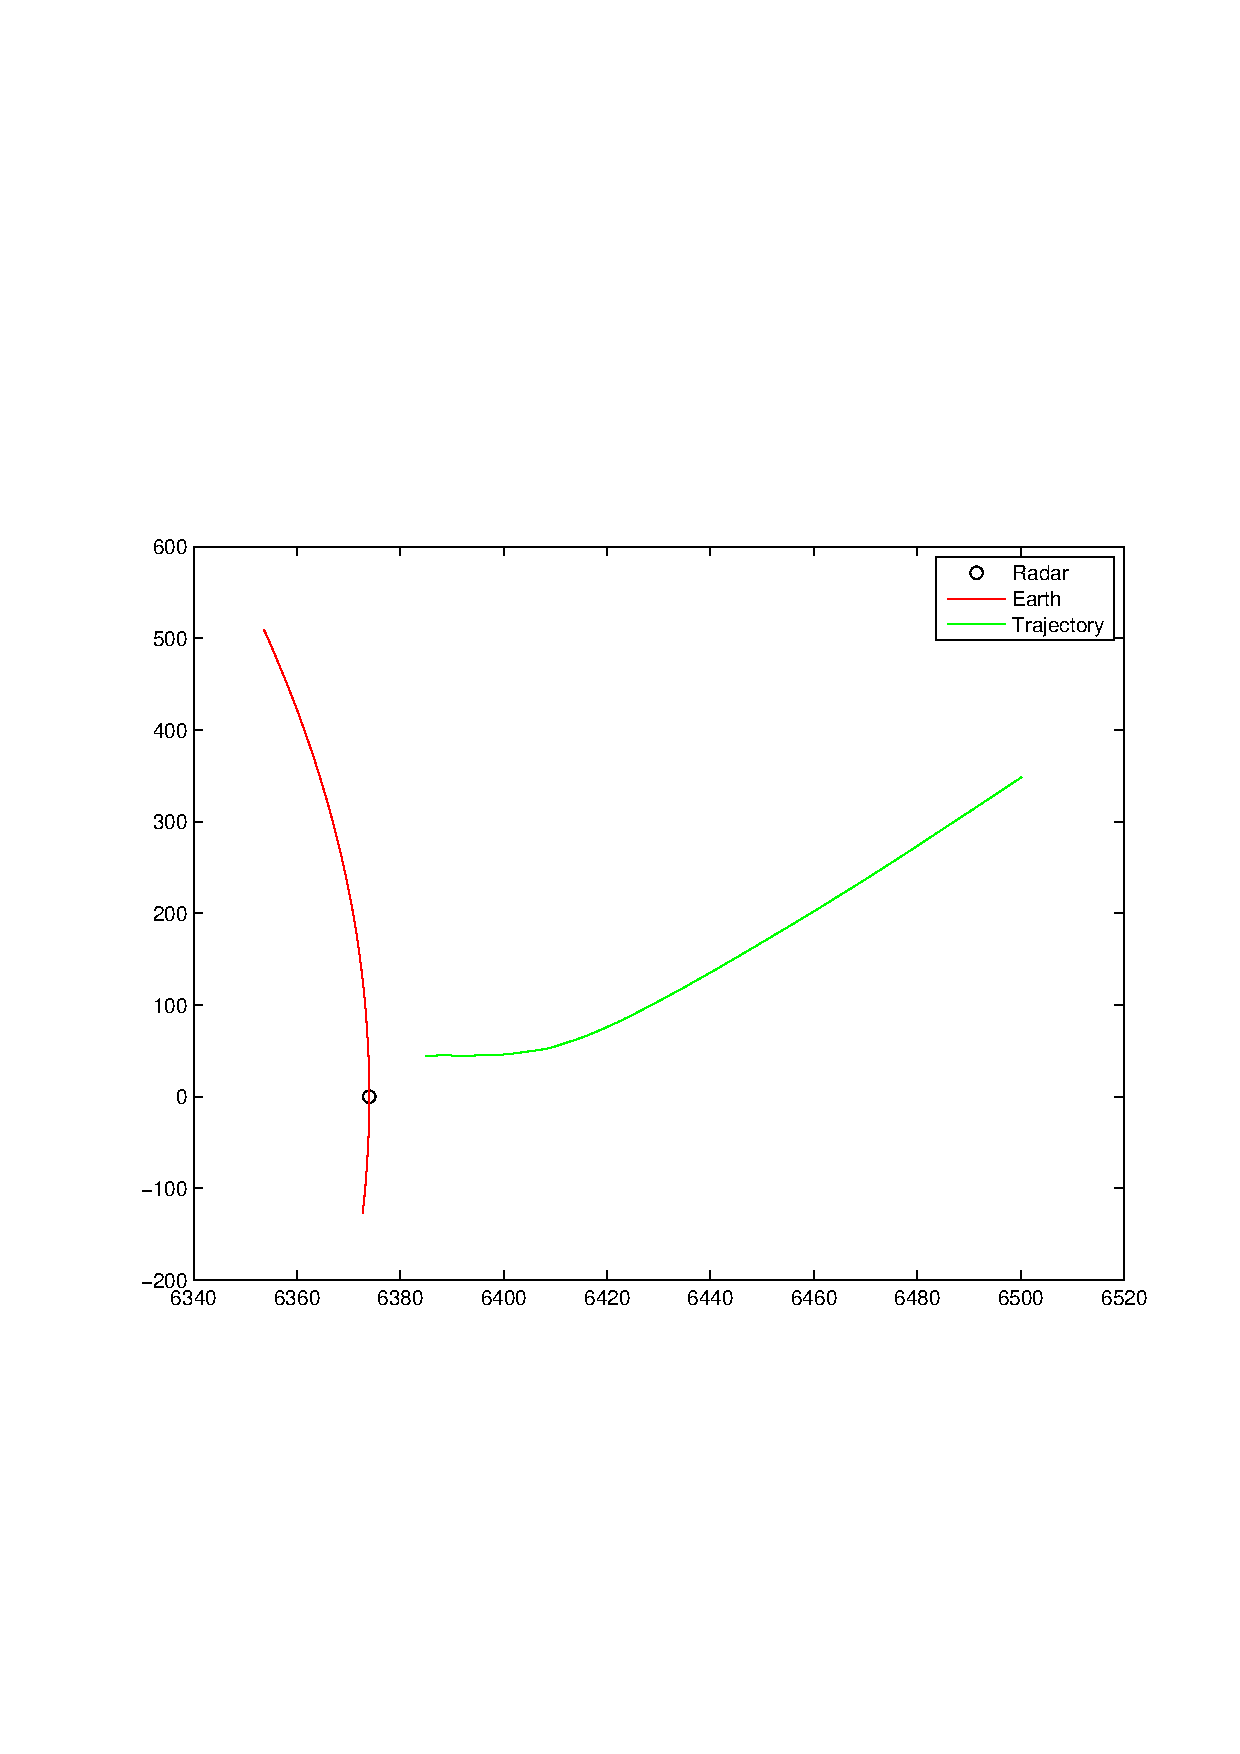
\includegraphics[width=11cm]{pics/reentry_trajectory}
\caption{Sample vehicle trajectory, earth and position of radar in
Reentry Vehicle Tracking problem.}
\label{fig:reentry_traj}
\end{center}
\end{figure}

In the table \ref{table:reentry_rmse} we have listed the RMS errors of
position estimates with tested methods, which were
%
\begin{itemize}
%
\item EKF1: first order extended Kalman filter.
\item ERTS: first order Rauch-Tung-Striebel smoother.
\item UKF: augmented form unscented Kalman filter.
\item URTS1: unscented Rauch-Tung-Striebel smoother with non-augmented
sigma points.
\item URTS2: unscented Rauch-Tung-Striebel smoother with augmented
sigma points.
\item UTF: unscented Forward-Backward smoother.
%
\end{itemize}
%
Extended Forward-Backward smoother was also tested, but it produced in
many cases divergent estimates, so it was left out from
comparison. Second order EKF was also left out, because evaluating the
Hessians would have taken too much work while considering the fact,
that the estimates might have gotten even worse.

From the error estimates we can see, that EKF and UKF --- and the
other methods as well --- give almost
identical performances, altough in the article \citep{Julier+Uhlmann:2004} UKF was clearly superior over EKF. The reason for this might be
the fact that they used numerical approximations (central differences)
for calculating the Jacobian in EKF rather than calculating the
derivatives in closed form, as was done in this demonstration.

In figure \ref{fig:reentry_errors} we have plotted the mean square
errors and variances in estimating $x_1$, $x_3$ and $x_5$ with EKF and
ERTS over 100 Monte Carlo runs. It shows that using smoother always
gives better estimates for positions and velocities, but for $x_5$ the
errors are practically the same after $\sim 45$ seconds. This also
shows that both methods are pessimistic in estimating $x_5$, because
variances were bigger than the true errors. Figures for $x_2$ and
$x_4$ are not shown, because they are very similar to the ones of
$x_1$ and $x_3$. Also by using UKF and URTS the resulting figures were
in practically identical, and therefore left out.
% 
%  
\begin{table}
\begin{center}
\begin{tabular}{|l|l|} \hline {\it Method}&{\it RMSE } \\ \hline
 EKF1  & 0.0084 \\ 
 ERTS  & 0.0044 \\ 
 UKF   & 0.0084 \\ 
 URTS1 & 0.0044 \\ 
 URTS2 & 0.0044 \\ 
 UTF   & 0.0044 \\
 GHKF  & 0.0084 \\
 GHRTS & 0.0049 \\
 CKF   & 0.0084 \\
 CRTS  & 0.0049 \\
 \hline
\end{tabular}
\caption{Average RMSEs of estimating the position in Reentry Vehicle
Tracking problem over 100 Monte Carlo runs. The Gauss--Hermite rule is
of degree 3.}
\label{table:reentry_rmse}
\end{center}
\end{table}
%
\begin{figure}
\begin{center}
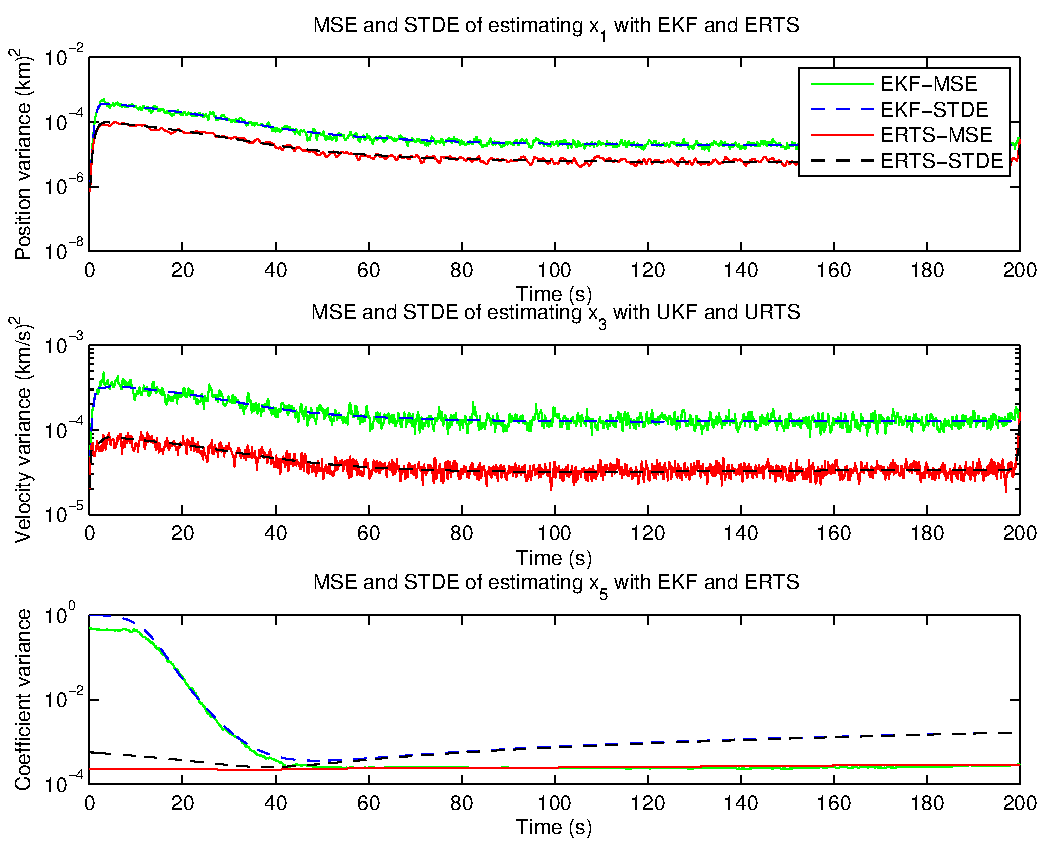
\includegraphics[width=11cm]{pics/reentry_errors}
\caption{MSEs and variances in estimating of $x_1$, $x_3$ and $x_5$
using EKF and ERTS over 100 Monte Carlo runs.}
\label{fig:reentry_errors}
\end{center}
\end{figure}



%
%%%%%%%%%%%%%%%%%%%%%%%%%%%%%%%%%%%%%%%%%%%%%%%%%%%%%%%%%%%%%%%%%%%%%%%%%%%%%%

\clearpage
\newpage




%%%%%%%%%%%%%%%%%%%%%%%%%%%%%%%%%%%%%%%%%%%%%%%%%%%%%%%%%%%%%%%%%%%%%%%%%%%%%%
%
  \chapter{Multiple Model Systems}
\label{ch:IMM}

In many practical scenarios it is reasonable to assume that the the
system's model can change through time somehow. For example, a fighter
airplane, which in normal situation flies with stabile flight
dynamics, might commence rapid maneuvers when approached by a hostile
missile, or a radar can have a different SNR in some regions of space
than in others, and so on. Such varying system characteristics are
hard to describe with only a one certain model, so in estimation one
should somehow take into account the possibility that the system's
model might change.

We now consider systems, whose current model is one from a discrete
set of $n$ models, which are denoted by $M = \{M^1,\ldots,M^n\}$. We
assume that for each model $M^j$ we have some prior probability
$\mu_0^j = P\{M_0^j\}$. Also the probabilities of switching from model
$i$ to model $j$ in next time step are assumed to be known and denoted
by $p_{ij} = P\{M_k^j|M_{k-1}^i\}$. This can be seen as a transition
probability matrix of a first order Markov chain characterizing the
mode transitions, and hence systems of this type are commonly referred
as {\it Markovian switching systems}. The optimal approach to
filtering the states of multiple model system of this type requires
running optimal filters for every possible model sequences, that is,
for $n$ models $n^k$ optimal filters must be ran to process the $k$th
measurement. Hence, some kind of approximations are needed in
practical applications of multiple model systems.

% One approach to handling the large number of hypotheses in the %
filtering problems is the Generalized Pseudo-Bayesian (GPB) %
algorithms ( In this section we describe the Interacting Multiple
Model (IMM) filter \citep{Bar-Shalom+Li+Kirubarajan:2001}, which is a popular
method for estimating systems, whose model changes according to a
finite-state, discrete-time Markov chain. IMM filter can also be used
in situations, in which the unknown system model structure or it's
parameters are estimated from a set of candidate models, and hence it
can be also used as a method for model comparison.

As previously we start with linear models, and after that we review
the EKF and UKF based nonlinear extensions to the standard IMM-filter
through demonstrating filtering problems.


\section{Linear Systems}

We can now modify the equations of linear systems described in
(\ref{eq:kalman_model}) to have form
%
\begin{equation}
\begin{split} \vec{x}_{k} &= \mat{A}_{k-1}^j \, \vec{x}_{k-1} +
\vec{q}_{k-1}^j \\ \vec{y}_{k} &= \mat{H}_{k}^j \, \vec{x}_{k} +
\vec{r}_{k}^j,
\end{split}
\label{eq:imm_lin_model}
\end{equation}
%
where now we have denoted by $j$ the model (or mode) which is in
effect during the time step $k-1$. Conditioned on the currently active
mode we can use the classical Kalman filter (section 2.1.2) for
estimating the state of the system on each time step. However, the
active mode of the system is not usually known, so we must estimate it
also.

\subsection{Interacting Multiple Model Filter}

IMM-filter \citep{Bar-Shalom+Li+Kirubarajan:2001} is a computationally efficient
and in many cases well performing suboptimal estimation algorithm for
Markovian switching systems of type described above. Basically it
consists of three major steps: interaction (mixing), filtering and
combination. In each time step we obtain the initial conditions for
certain model-matched filter by mixing the state estimates produced by
all filters from the previous time step under the assumption that this
particular model is the right model at current time step. Then we
perform standard Kalman filtering for each model, and after that we
compute a weighted combination of updated state estimates produced by
all the filters yielding a final estimate for the state and covariance
of the Gaussian density in that particular time step. The weights are
chosen according to the probabilities of the models, which are
computed in filtering step of the algorithm.

The equations for each step are as follows:

\begin{itemize}

\item {\em Interaction:}
  
  The mixing probabilities $\mu_k^{i|j}$ for each model $M^i$ and
$M^j$ are calculated as
  %
  \begin{eqnarray}
  % 
  \bar{c}_j & = & \sum_{i=1}^n p_{ij} \mu_{k-1}^i,\\ \label{eq:imm_cj}
\mu_k^{i|j} & = & \frac{1}{\bar{c}_j} p_{ij} \mu_{k-1}^i,
  % 
  \end{eqnarray}
  %
  where $\mu_{k-1}^i$ is the probability of model $M^i$ in the time
step $k-1$ and $\bar{c}_j$ a normalization factor.

  Now we can compute the mixed inputs (that is, means and covariances)
for each filter as
  %
  \begin{eqnarray}
  %
  \vec{m}_{k-1}^{0j} & = & \sum_{i=1}^n \mu_k^{i|j} \vec{m}_{k-1}^i,
\\
  %
  \mat{P}_{k-1}^{0j} & = & \sum_{i=1}^n \mu_k^{i|j} \times \left\{
\mat{P}_{k-1}^i +
\left[\vec{m}_{k-1}^i-\vec{m}_{k-1}^{0j}\right]\left[\vec{m}_{k-1}^i-\vec{m}_{k-1}^{0j}\right]^T\right\},
  %
  \end{eqnarray}
  %
  where $\vec{m}_{k-1}^i$ and $\mat{P}_{k-1}^i$ are the updated mean
and covariance for model $i$ at time step $k-1$.

\item {\em Filtering:}

  Now, for each model $M^i$ the filtering is done as
  %
  \begin{eqnarray}
  %
  \left[\vec{m}_{k}^{-,i},\mat{P}_{k}^{-,i}\right] & = &
\text{KF}_p(\vec{m}_{k-1}^{0j},\mat{P}_{k-1}^{0j},\mat{A}_{k-1}^i,\mat{Q}_{k-1}^i)
, \\ \label{eq:imm_predict}
  % 
  \left[\vec{m}_{k}^{i},\mat{P}_{k}^{i}\right] & = &
\text{KF}_u(\vec{m}_{k}^{-,i},\mat{P}_{k}^{-,i},\vec{y}_{k},\mat{H}_{k}^i,\mat{R}_{k}^i),
\label{eq:imm_update}
  % 
  \end{eqnarray}
  %
  where we have denoted the prediction and update steps (equations
(\ref{eq:dkf_predict}) and (\ref{eq:dkf_update})) of the standard
Kalman filter with $\text{KF}_p(\cdot)$ and $\text{KF}_u(\cdot)$,
correspondingly. In addition to mean and covariance we also compute
the likelihood of the measurement for each filter as
  %
  \begin{equation}
  %
  \Lambda_k^i = \text{N}(\vec{v}_k^i;0,\mat{S}_k^i),
  %
  \end{equation}
  % 
  where $\vec{v}_k^i$ is the measurement residual and $\mat{S}_k^i$
it's covariance for model $M^i$ in the KF update step.

  The probabilities of each model $M^i$ at time step $k$ are
calculated as
  %
  \begin{eqnarray}
  %
  c & = & \sum_{i=1}^n \Lambda_k^i \bar{c}_i, \\ \label{eq:imm_c}
\mu_k^i & = & \frac{1}{c} \Lambda_k^i \bar{c}_i, \label{eq:imm_muk}
  %
  \end{eqnarray}
  % 
  where $c$ is a normalizing factor.

\item {\em Combination:}
  
  In the final stage of the algorithm the combined estimate for the
state mean and covariance are computed as
  %
  \begin{eqnarray}
  %
  \vec{m}_k & = & \sum_{i=1}^n \mu_k^i \vec{m}_{k}^{i}, \\
  %
  \mat{P}_k & = & \sum_{i=1}^n \mu_k^i \times \left\{\mat{P}_{k}^{i}
\left[\vec{m}_{k}^{i} -\vec{m}_k\right] \left[\vec{m}_{k}^{i}
-\vec{m}_k\right]^T\right\}.
  %
  \end{eqnarray}
  %
  
\end{itemize}

In this toolbox prediction and updates steps of the IMM-filter can be
computed with functions \texttt{imm\_kf\_predict} and
\texttt{imm\_kf\_update}. For convience we have also provided function
\texttt{imm\_filter}, which combines the two previously mentioned
steps.


\subsection{Interacting Multiple Model Smoother}

Likewise in the single model case also it is useful to smooth the
state estimates of the IMM filter by using all the obtained
measurements. Since the optimal fixed-interval smoothing with $n$
models and $N$ measurements requires running $n^N$ smoothers we must
resort to suboptimal approaches. One possibility \citep{Helmick+Blair+Hoffman:1995} is to
combine the estimates of two IMM filters, one running forwards and the
other backwards in time. This approach is restricted to systems having
invertible state dynamics (i.e. system for which the inverse of matrix
$\mat{A}^j$ in (\ref{eq:imm_lin_model}) exists), which is always the
case for discretized continuous-time systems.

First we shall review the equations for the IMM-filter running
backwards in time, and then the actual smoothing equations combining
the estimates of the two filters.

\subsection*{Backward-time IMM-filter}

Our aim is now to compute the backward filtering density
$p(\vec{x}_k|\vec{y}_{k:N})$ for each time step, which is expressed as
a sum of model conditioned densities:
% 
\begin{equation}
  % 
  p(\vec{x}_k|\vec{y}_{k:N}) = \sum_{j=1}^{n} \mu_k^{b,j}
p(\vec{x}_k^j|\vec{y}_{k:N}), \label{eq:imm_backward_total_density}
  % 
\end{equation}
% 
where $\mu_k^{b,j}$ is the backward-time filtered model probability of
$M_k^j$. In the last time step $N$ this is the same as the forward
filter's model probability, that is, $\mu_N^{b,j} =
\mu_N^{j}$. Assuming the model conditioned densities
$p(\vec{x}_k^j|\vec{y}_{k:N})$ are Gaussians the backward density in
(\ref{eq:imm_backward_total_density}) is a mixture of Gaussians, which
is now going to be approximated with a single Gaussian via moment
matching.

The model conditioned backward-filtering densities can be expressed as
%
\begin{equation}
%
p(\vec{x}_k^j|\vec{y}_{k:N}) = \frac{1}{c}
p(\vec{y}_{k:N}|\vec{x}_k^j) p(\vec{x}_k^j|\vec{y}_{k+1:N}),
%
\end{equation}
%
where $c$ is some normalizing constant, $p(\vec{y}_{k:N}|\vec{x}_k^j)$
the model-conditioned measurement likelihood and
$p(\vec{x}_k^j|\vec{y}_{k+1:N})$ is the model-conditioned density of
the state given the future measurements.  The latter density is
expressed as
%
\begin{equation}
%
p(\vec{x}_k^j|\vec{y}_{k+1:N}) = \sum_{i=1}^n \mu_{k+1}^{b,i|j}
p(\vec{x}_k^j|M_{k+1}^i,\vec{y}_{k+1:N}),
\label{eq:imm_back_modelc_predict}
%
\end{equation}
%
where $\mu_{k+1}^{b,i|j}$ is the conditional model probability
computed as
%
\begin{eqnarray}
%
\mu_{k+1}^{b,i|j} & = & P\{M_{k+1}^i|M_k^j,\vec{y}_{k+1:N} \} \\
\label{eq:imms_cond_mod_prob} & = & \frac{1}{a_j} p_{ij}^{b,k}
\mu_{k+1}^{b,i},
%
\end{eqnarray}
%
where $a_j$ is a normalization constant given by
%
\begin{equation}
%
a_j = \sum_{i=1}^{n} p_{ij}^{b,k}
\mu_{k+1}^{b,i}. \label{eq:imms_constant_a}
%
\end{equation}
%
The backward-time transition probabilities of switching from model
$M_{k+1}^i$ to model $M_k^j$ in (\ref{eq:imms_cond_mod_prob}) and
(\ref{eq:imms_constant_a}) are defined as $p_{ij}^{b,k} =
P\{M_k^j|M_{k+1}^i\}$. The prior model probabilities can be computed
off-line recursively for each time step $k$ as
%
\begin{eqnarray}
%
P\{M_k^j\} & = & \sum_{i=1}^n P\{M_k^j|M_{k-1}^i\} P\{M_{k-1}^i\} \\ &
= & \sum_{i=1}^n p_{ij} P\{M_{k-1}^i\}
%
\end{eqnarray}
%
and using these we can compute $p_{ij}^{b,k}$ as
%
\begin{equation}
%
p_{ij}^{b,k} = \frac{1}{b_i} p_{ji} P\{M_{k}^j\},
%
\end{equation}
%
where $b_i$ is the normalizing constant
%
\begin{equation}
%
b_i = \sum_{j=1}^n p_{ji} P \{ M_k^j\}.
%
\end{equation}
%

The density $p(\vec{x}_k^j|M_{k+1}^i,\vec{y}_{k+1:N}^N)$ is now
approximated with a Gaussian
$N(\vec{x}_k|\vec{m}_{k|k+1}^{b,i},\mat{P}_{k|k+1}^{b,-(i)})$, where
the mean and covariance are given by the Kalman filter prediction step
using the inverse of the state transition matrix:
%
\begin{equation}
%
  \left[\vec{\hat{m}}_{k}^{b,i},\mat{\hat{P}}_{k}^{b,i}\right] =
\text{KF}_p(\vec{m}_{k+1}^{b,i},\mat{P}_{k+1}^{b,i},(\mat{A}_{k+1}^i)^{-1},\mat{Q}_{k+1}^i). \label{eq:imm_b_predict}
%
\end{equation}
%
The density $p(\vec{x}_k^j|\vec{y}_{k+1:N})$ in
(\ref{eq:imm_back_modelc_predict}) is a mixture of Gaussians, and it's
now approximated with a single Gaussian as
%
\begin{equation}
%
p(\vec{x}_k^j|\vec{y}_{k+1:N}) =
N(\vec{x}_k^j|\vec{\hat{m}}_{k}^{b,0j},\mat{\hat{P}}_{k}^{b,0j}),
%
\end{equation}
%
where the mixed predicted mean and covariance are given as
%
\begin{eqnarray}
%
\vec{\hat{m}}_{k}^{b,0j} & = & \sum_{i=1}^n \mu_{k+1}^{b,i|j}
\vec{\hat{m}}_{k}^{b,i} \\
%
\mat{\hat{P}}_{k}^{b,0j} & = & \sum_{i=1}^n \mu_{k+1}^{b,i|j} \cdot
\left[ \mat{\hat{P}}_{k}^{b,i} +\left( \vec{\hat{m}}_{k}^{b,i} -
\vec{\hat{m}}_{k}^{b,0j} \right) \left( \vec{\hat{m}}_{k}^{b,i} -
\vec{\hat{m}}_{k}^{b,0j} \right)^T\right]
%
\end{eqnarray}
%

Now, the filtered density $p(\vec{x}_k^j|\vec{y}_{k:N})$ is a Gaussian
$N(\vec{x}_k|\vec{m}_{k}^{b,j},\mat{P}_{k}^{b,j})$, and solving it's
mean and covariance corresponds to running the Kalman filter update
step as follows:
%
\begin{equation}
%
  \left[\vec{m}_{k}^{b,j},\mat{P}_{k}^{b,j}\right] =
\text{KF}_u(\vec{\hat{m}}_{k}^{b,0j},\mat{\hat{P}}_{k}^{b,0j},\vec{y}_k,\mat{H}_k^j,\mat{R}_k^j). \label{eq:imm_b_update}
%
\end{equation}
%
The measurement likelihoods for each model are computed as
% 
\begin{equation}
  % 
  \Lambda_k^{b,i} = \text{N}(\vec{v}_k^{b,i};0,\mat{S}_k^{b,i}),
  % 
\end{equation}
  % 
where $\vec{v}_k^{b,i}$ is the measurement residual and
$\mat{S}_k^{b,i}$ it's covariance for model $M^i$ in the KF update
step.
%
With these we can update the model probabilities for time step $k$ as
%
\begin{equation}
%
\mu_k^{b,j} = \frac{1}{a} a_j \Lambda_k^{b,i},
%
\end{equation}
%
where $a$ is a normalizing constant
%
\begin{equation}
%
a = \sum_{j=1}^{m} a_j \Lambda_k^{b,i}.
%
\end{equation}
%
Finally, we can form the Gaussian approximation to overall backward
filtered distribution as
%
\begin{equation}
%
p(\vec{x}_k|\vec{y}_{k:N}) = N(\vec{x}_k|\vec{m}_k^b,\mat{P}_{k}^b),
%
\end{equation}
%
where the mean and covariance are mixed as
%
\begin{eqnarray}
%
\vec{m}_k^b & = & \sum_{j=1}^n \mu_k^{b,j} \vec{m}_k^{b,j} \\
%
\mat{P}_{k}^b & = & \sum_{j=1}^{n} \mu_k^{b,j} \left[ \mat{P}_k^{b,j}
+ \left( \vec{m}_k^{b,j} - \vec{m}_k^{b} \right) \left(
\vec{m}_k^{b,j} - \vec{m}_k^{b}\right)^T \right].
%
\end{eqnarray}
%

\subsection{Two-filter based fixed-interval IMM-Smoother}

We can now proceed to evaluate the fixed-interval smoothing
distribution
%
\begin{equation}
%
p(\vec{x}_k|\vec{y}_{1:N}) = \sum_{j=1}^n \mu_k^{s,j}
p(\vec{x}_k^j|\vec{y}_{1:N}), \label{eq:imm_smooth_density}
%
\end{equation}
%
where the smoothed model probabilities are computed as
%
\begin{eqnarray}
%
\mu_k^{s,j} & = & P\{ M_k^j|\vec{y}_{1:N}\} \\ & = & \frac{1}{d} d_j
\mu_k^j,
%
\end{eqnarray}
%
where $\mu_k^j$ is the forward-time filtered model probability, $d_j$
the density $d_j = p(\vec{y}_{k+1:N}|M_k^j,\vec{y}_{1:k})$ (which is
to be evaluated later) and $d$ the normalization constant given by
%  
\begin{equation}
%
d = \sum_{j=1}^{n} d_j \mu_k^j.
%
\end{equation}
%

The model-conditioned smoothing distributions
$p(\vec{x}_k^j|\vec{y}_{1:N})$ in \eqref{eq:imm_smooth_density} are
expressed as a mixtures of Gaussians
%
\begin{equation}
%
p(\vec{x}_k^j|\vec{y}_{1:N}) = \sum_{i=1}^{n} \mu_{k+1}^{s,i|j}
p(\vec{x}^i|M_{k+1}^j,\vec{y}_{1:n}), \label{eq:imm_smooth_modelcs}
%
\end{equation}
%
where the conditional probability $\mu_{k+1}^{s,i|j}$ is given by
%
\begin{eqnarray}
%
\mu_{k+1}^{s,i|j} & = & P\{ M_{k+1}^i| M_k^j, \vec{y}_{1:n}\} \\ & = &
\frac{1}{d_j} p_{ji} \Lambda_k^{ji}
%
\end{eqnarray}
%
and the likelihood $\Lambda_k^{ji}$ by
%
\begin{equation}
%
\Lambda_k^{ji} = p(\vec{y}_{k+1:N}|M_k^j,M_{k+1}^i,\vec{y}_{1:k}).
%
\end{equation}
%
We approximate this now as
%
\begin{equation}
%
\Lambda_k^{ji} \approx
p(\vec{\hat{x}}_k^{b,i}|M_k^j,M_{k+1}^i,\vec{x}_{k}^j),
%
\end{equation}
%
which means that the future measurements $\vec{y}_{k+1:N}$ are
replaced with the $n$ model-conditioned backward-time one-step
predicted means and covariances
$\{\vec{\hat{m}}_k^{b,i},\vec{\hat{P}}_k^{b,i}\}_{r=1}^{n}$, and
$\vec{y}_{1:k}$ will be replaced by the $n$ model-conditioned
forward-time filtered means and covariances
$\{\vec{m}_k^{i}|\vec{P}_k^{i}\}_{r=1}^{n}$. It follows then that the
likelihoods can be evaluated as
%
\begin{equation}
%
\Lambda_k^{ji} = N(\Delta_k^{ji}|0,D_k^{ji}),
%
\end{equation}
%
where
%
\begin{eqnarray}
%
\Delta_k^{ji} & = & \vec{\hat{m}}_k^{b,i} - \vec{m}_k^j \\
%
D_k^{ji} & = & \vec{\hat{P}}_k^{b,i} + \vec{P}_k^j.
%
\end{eqnarray}
%
The terms $d_j$ can now be computed as
%
\begin{equation}
%
d_j = \sum_{i=1}^n p_{ji} \Lambda_k^{ji}.
%
\end{equation}
% 
The smoothing distribution $p(\vec{x}_k^j|M_{k+1}^i,\vec{y}_{1:N})$ of
the state matched to the models $M_k^j$ and $M_{k+1}^i$ over two
successive sampling periods can be expressed as
%
\begin{equation}
%
p(\vec{x}_k^j|M_{k+1}^i,\vec{y}_{1:N}) = \frac{1}{c}
p(\vec{y}_{k+1:N}|M_{k+1}^i,\vec{x}_k) p(\vec{x}_k^j|\vec{y}_{1:k}),
%
\end{equation}
% 
where $p(\vec{y}_{k+1:N}|M_{k+1}^i,\vec{x}_k)$ is the forward-time
model-conditioned filtering distribution,
$p(\vec{x}_k^j|\vec{y}_{1:k})$ the backward-time one-step predictive
distribution and $c$ a normalizing constant. Thus, the smoothing
distribution can be expressed as
%
\begin{eqnarray}
%
p(\vec{x}_k^j|M_{k+1}^i,\vec{y}_{1:N}) & \propto&
N(\vec{x}_k|\vec{\hat{m}}_k^{b,i},\vec{\hat{P}}_k^{b,i}) \cdot
N(\vec{x}_k|\vec{m}_k^{i},\vec{P}_k^{i}) \\ & = &
N(\vec{x}_k|\vec{m}_k^{s,ji},\vec{P}_k^{s,ji}),
%
\end{eqnarray}
%
where
% 
\begin{eqnarray}
%  
\vec{m}_k^{s,ji} & = & \mat{P}_k^{s,ji} \left[
\left(\vec{P}_k^{i}\right)^{-1}\vec{m}_k^{i} +
\left(\vec{\hat{P}}_k^{b,i}\right)^{-1}\vec{\hat{m}}_k^{b,i} \right]
\\
%
\mat{P}_k^{s,ji} & = & \left[ \left(\vec{P}_k^{i}\right)^{-1} +
\left(\vec{\hat{P}}_k^{b,i}\right)^{-1} \right]^{-1}.
%
\end{eqnarray}
%

The model-conditioned smoothing distributions
$p(\vec{x}_k^j|\vec{y}_{1:N})$, which were expressed as mixtures of
Gaussians in \eqref{eq:imm_smooth_modelcs}, are now approximated by a
single Gaussians via moment matching to yield
%
\begin{equation}
%
p(\vec{x}_k^j|\vec{y}_{1:N}) \approx
N(\vec{x}_k^j|\vec{m}_k^{s,j},\mat{P}_k^{s,j}),
%
\end{equation}
%
where
%
\begin{eqnarray}
%
\vec{m}_k^{s,j} & = & \sum_{i=1}^{n} \mu_{k+1}^{s,i|j}
\vec{m}_k^{s,ji} \\
%
\mat{P}_k^{s,j} & = & \sum_{i=1}^n \mu_{k+1}^{s,i|j} \cdot \left[
\mat{P}_{k}^{s,ij} + \left( \vec{m}_{k}^{s,ij} - \vec{m}_{k}^{s,j}
\right) \left( \vec{m}_{k}^{s,ij} - \vec{m}_{k}^{s,j}
\right)^T\right].
%
\end{eqnarray}
%
With these we can match the moments of the overall smoothing
distribution to give a single Gaussian approximation
%
\begin{equation}
%
p(\vec{x}_k|\vec{y}_{1:N}) \approx
N(\vec{x}_k|\vec{m}_k^s,\mat{P}_k^s),
%
\end{equation}
%
where
%
\begin{eqnarray}
%
\vec{m}_k^s & = & \sum_{j=1}^{n} \mu_{k}^{s,j} \vec{m}_k^{s,ji} \\
%
\mat{P}_k^{s} & = & \sum_{j=1}^n \mu_{k}^{s,j} \cdot \left[
\mat{P}_{k}^{s,j} + \left( \vec{m}_{k}^{s,j} - \vec{m}_k^s \right)
\left( \vec{m}_{k}^{s,j} - \vec{m}_k^s \right)^T\right].
%
\end{eqnarray}
%

These smoothing equations can be computed with function
\texttt{imm\_smooth}.

\subsection{Demonstration: Tracking a Target with Simple Manouvers}

A moving object with simple manouvers can be modeled by a Markovian
switching system, which describes the normal movement dynamics with a
simple Wiener process velocity model (see section 2.2.9) with low
process noise value, and the manouvers with a Wiener process
acceleration model (see section 2.1.4) with high process noise
value. In the following we shall refer the former as model 1 and the
latter as the model 2, which could actually also be a velocity model,
but we use acceleration model instead to demonstrate how models with
different structure are used in this toolbox.

The variance of process noise for model 1 is set to
%
\begin{equation} \mat{Q}_c^1 =
\begin{pmatrix} q_1 & 0 \\ 0 & q_1
\end{pmatrix} =
\begin{pmatrix} 0.01 & 0 \\ 0 & 0.01
\end{pmatrix}
\end{equation}
%
and for model 2 to
%
\begin{equation} \mat{Q}_c^2 =
\begin{pmatrix} q_2 & 0 \\ 0 & q_2
\end{pmatrix} =
\begin{pmatrix} 1 & 0 \\ 0 & 1
\end{pmatrix}
\end{equation}
%
In both cases the measurement model is the same as in the section
2.1.4 (that is, we observe the position of the object directly) with
the exception that the variance of the measurements is now set to
%
\begin{equation} \mat{R} = \begin{pmatrix} 0.1 & 0 \\ 0 & 0.1 \\
\end{pmatrix}.
\end{equation}
%
The time step size is set to $\dt = 0.1$. The true starting state of
the system is set to
%
\begin{equation}
%
\vec{x}_0 = \begin{bmatrix} 0 & 0 & 0 & -1& 0 & 0\end{bmatrix},
%
\end{equation}
%
which means that the object starts to move from origo with velocity
$-1$ along the y-axis.
%
The model transition probability matrix is set to
%
\begin{equation}
%
\mat{\Phi} =
\begin{pmatrix} 0.98 & 0.02 \\ 0.02 & 0.98
\end{pmatrix}, \label{eq:imm_mtpm}
%
\end{equation}
%
which means that both models have equal probability of shifting to
another model during each sampling period. The prior model
probabilities are set to
%
\begin{equation}
%
\vec{\mu}_0 = \begin{bmatrix} 0.9 & 0.1
\end{bmatrix}. \label{eq:imm_modelprior}
%
\end{equation}
%

In software code the filtering loop of IMM filter can be done as
follows:
%
\begin{lstlisting} 
for i = 1:size(Y,2) 
  [x_p,P_p,c_j] = imm_predict(x_ip,P_ip,mu_ip,p_ij,ind,dims,A,Q); 
  [x_ip,P_ip,mu_ip,m,P] = imm_update(x_p,P_p,c_j, ...
    ind,dims,Y(:,i),H,R); 
  MM(:,i) = m;
  PP(:,:,i) = P; 
  MU(:,i) = mu_ip'; 
  MM_i(:,i) = x_ip'; 
  PP_i(:,i) = P_ip';
end
\end{lstlisting}
%
The variables \texttt{x\_ip} and \texttt{P\_ip} contain the updated
state mean and covariance for both models as cell arrays. The cell
arrays are used because the size of the state variable can vary
between different models. For example, in this example the models have
4 and 6 state components.  Similarly, the variables \texttt{x\_p} and
\texttt{P\_p} contain the predicted state means and
covariances. Likewise, the model parameters (variables
\texttt{A},\texttt{Q},\texttt{H} and \texttt{R}) are all cell arrays
containing the corresponding model parameters for each model. The
variable \texttt{mu\_ip} contains the probability estimates of each
model as a regular array, which is initialized before the filtering
loop with the prior probabilities of models
(eq. \eqref{eq:imm_modelprior}). The variable \texttt{p\_ij} is the
model transition probability matrix \eqref{eq:imm_mtpm} as a regular
Matlab matrix. The vector \texttt{c\_j} contains the normalizing
constants computed during the prediction step (eq. \eqref{eq:imm_cj}),
which are needed during the update step in eqs. \eqref{eq:imm_c} and
\eqref{eq:imm_muk}. The variable \texttt{ind} is a cell array
containing vectors, which map the state variables of each model to
state variables of the original system under the study. For example,
for model 1 the vector is \texttt{[1 2 3 4]'} and for model 2
\texttt{[1 2 3 4 5 6]'}. The purpose of this might seem a bit unclear
for systems like these, but for more complex models we must know how
the state variables are connected as they are not always in the same
order and some components might be missing. The variable \texttt{dims}
contains the number of dimensions in the original system under the
study, which in this case is 6. The last five lines of code store the
estimation results for each time step.

The smoothing can be done with the function call
\begin{lstlisting} 
[SM,SP,SM_i,SP_i,MU_S] = imm_smooth(MM,PP,MM_i,PP_i,MU,p_ij, ...
  mu_0j,ind,dims,A,Q,R,H,Y);
\end{lstlisting} 
where the variable \texttt{mu\_0j} contains the prior
model probabilities. The overall smoothed state estimates are returned
in variables \texttt{SM} and \texttt{SP}, and the model-conditioned
smoothed estimates in variables \texttt{SM\_i} and \texttt{SP\_i}. The
variable \texttt{MU\_S} contains the calculated smoothed model
probabilities.

The system is simulated $200$ time steps, and the active model during
the steps $1-50$, $71-120$ and $151-200$ is set to model 1 and during
the steps $51-70$ and $121-150$ to model 2. The purpose of forcing the
model transitions instead of simulating them randomly is to produce
two manouvers, which can be used to demonstrate the properties of
IMM-filter. It also reflects the fact that in real problems we do not
know the model transition probability matrix accurately. The figures
\ref{fig:imm_kf1}, \ref{fig:imm_kf2} and \ref{fig:imm_imm} show the
true trajectory of the object and the measurements made of it. The two
manouvers can be clearly seen. Figures also show the filtering and
smoothing results produced by Kalman filter and (RTS) smoother using
the models 1 and 2 separately (figures \ref{fig:imm_kf1} and
\ref{fig:imm_kf2}, correspodingly) as well as the estimates produced
by the IMM filter and smoother (figure \ref{fig:imm_imm}).  In figure
\ref{fig:imm_model_probability} we have plotted the filtered and
smoothed estimates of the probabilities of model 1 in each time
step. It can be seen that it takes some time for the filter to respond
to model transitions. As one can expect, smoothing reduces this lag as
well as giving substantially better overall performance.

The illustrate the performance differences between different models we
have listed the MSE errors of position estimates for each model in the
table \ref{table:imm_rmse}. From these it can be seen that the
estimates of Kalman filter with model 1 are clearly much worse than
with model 2 or with the IMM filter. On the otherhand, the difference
between the KF with model 2 and the IMM filter is smaller, but still
significant in the favor of IMM. This is most likely due to fact that
model 2 is more flexible than model 1, so model 2 is better in the
regions of model 1 than model 1 in the regions of model 2. The bad
performance of the model 1 can be seen especially during the
manouvers. The IMM filter combines the properties of both models in a
suitable way, so it gives the best overall performance. The effect of
smoothing to tracking accuracy is similar with all models.

\begin{figure}
\begin{center}
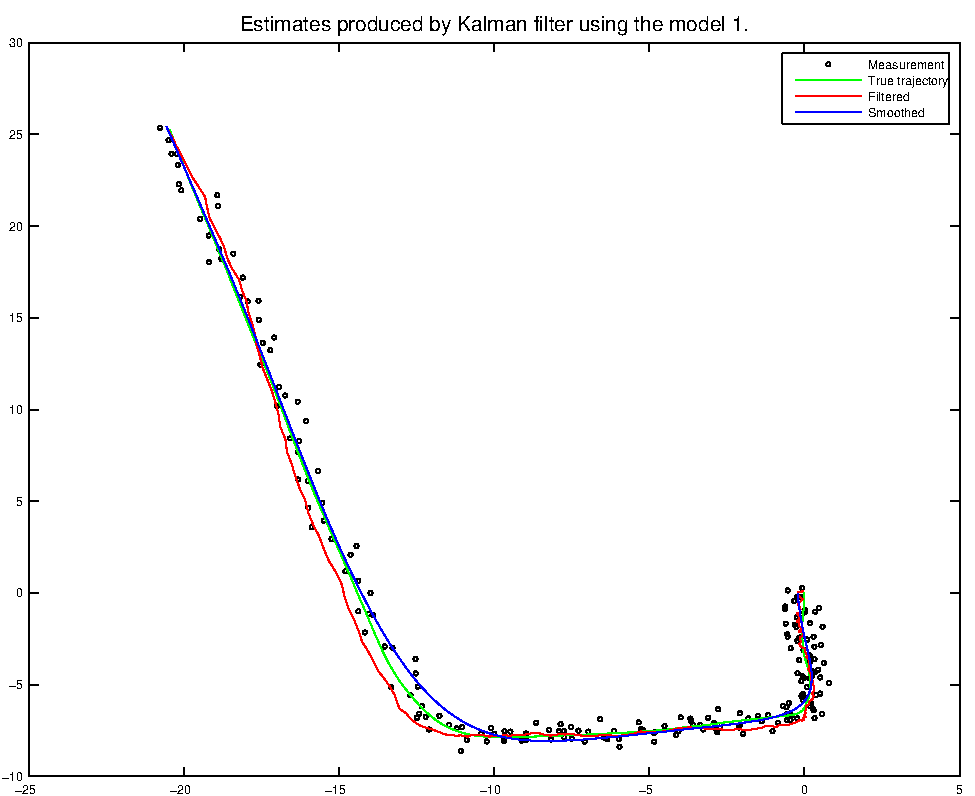
\includegraphics[width=11cm]{pics/imm1}
\caption{Tracking results of Kalman filter and smoother with model 1
in Tracking a Target with Simple Manouvers example.}
\label{fig:imm_kf1}
\end{center}
\end{figure}

\begin{figure}
\begin{center}
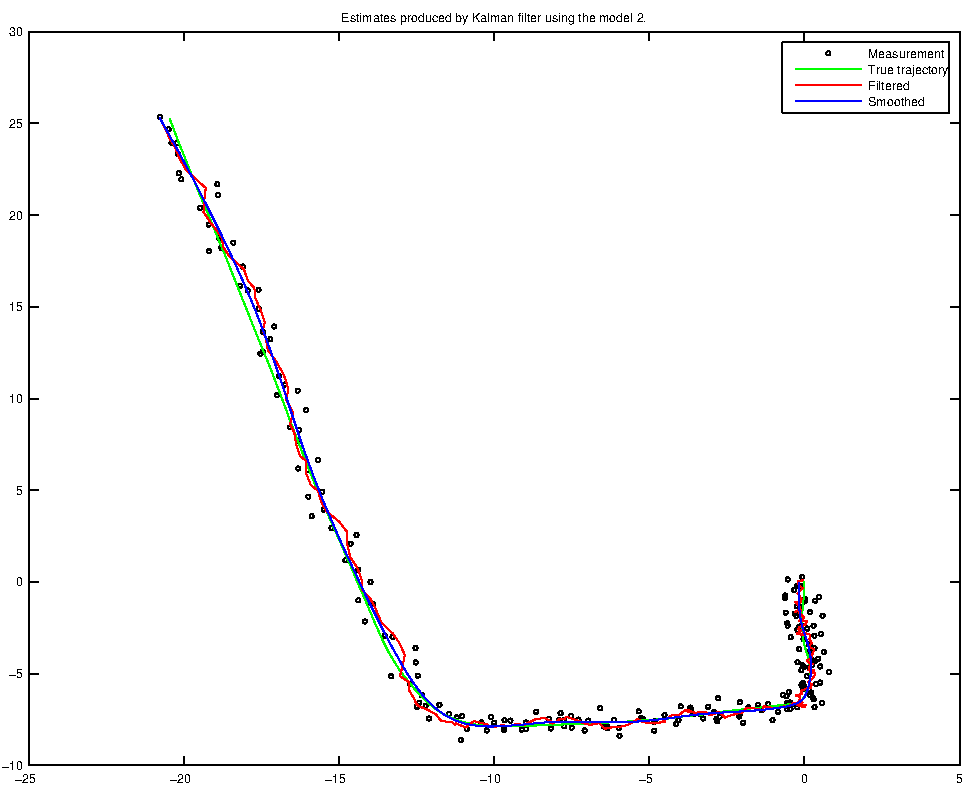
\includegraphics[width=11cm]{pics/imm2}
\caption{Tracking results of Kalman filter and smoother with model 2
in Tracking a Target with Simple Manouvers example.}
\label{fig:imm_kf2}
\end{center}
\end{figure}

\begin{figure}
\begin{center}
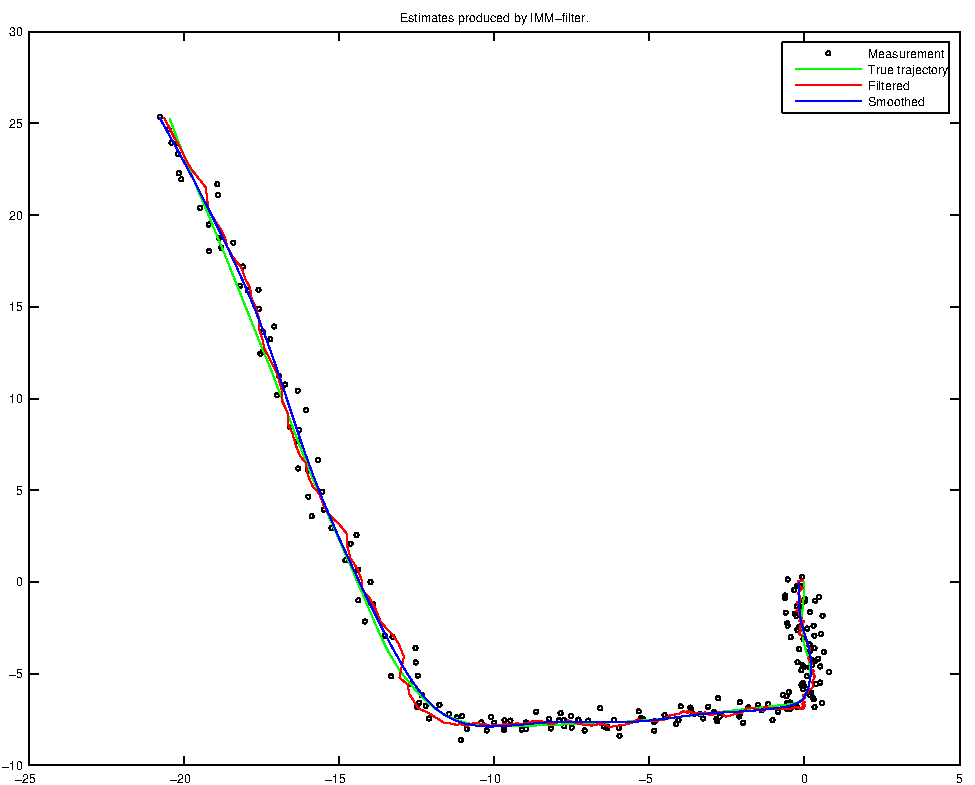
\includegraphics[width=11cm]{pics/imm3}
\caption{Tracking results of IMM filter and smoother in Tracking a
Target with Simple Manouvers example.}
\label{fig:imm_imm}
\end{center}
\end{figure}

\begin{figure}
\begin{center}
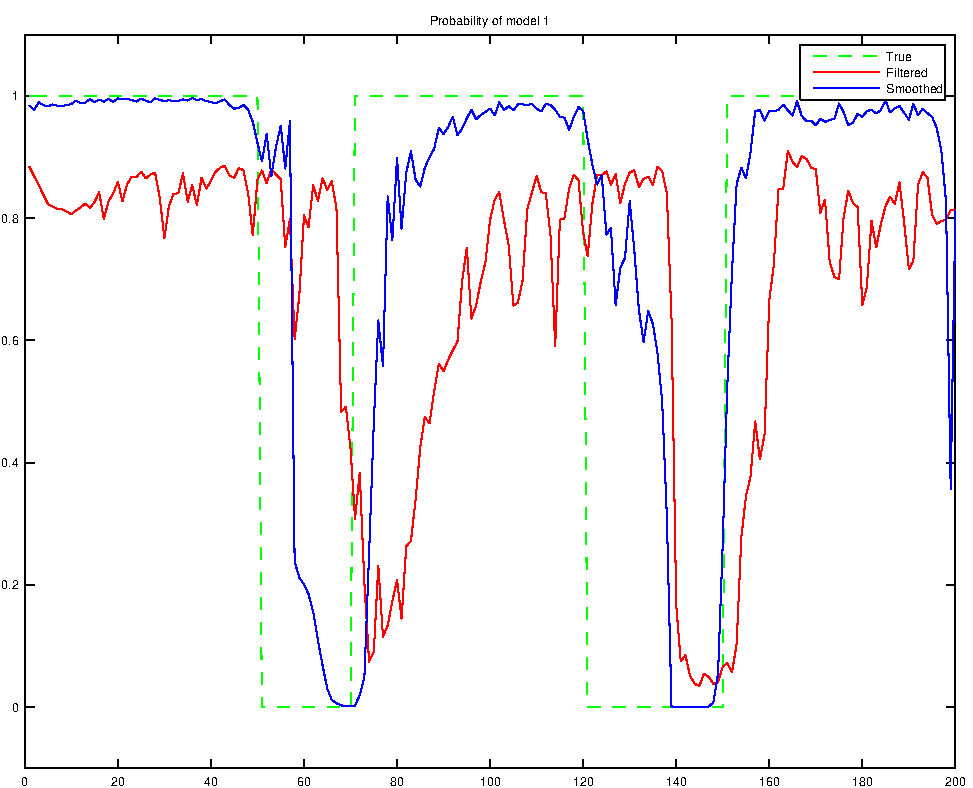
\includegraphics[width=11cm]{pics/imm4}
\caption{Filtered and smoothed probability of model 1 in each time
step in Tracking a Target with Simple Manouvers example.}
\label{fig:imm_model_probability}
\end{center}
\end{figure}

% 
%  
\begin{table}
\begin{center}
\begin{tabular}{|l|l|} \hline {\it Method}&{\it MSE } \\ \hline KF1 &
0.1554 \\ KS1 & 0.0314 \\ KF2 & 0.0317 \\ KS2 & 0.0071 \\ IMM & 0.0229
\\ IMMS & 0.0057 \\ \hline
\end{tabular}
\caption{Average MSEs of estimating the position in Tracking a Target
with Simple Manouvers example over 1000 Monte Carlo runs.}
\label{table:imm_rmse}
\end{center}
\end{table}
%

\section{Nonlinear Systems}

The non-linear versions of IMM filter and smoother reviewed in
previous section can be obtained simply by replacing the Kalman filter
prediction and update steps (in eqs. \eqref{eq:imm_predict},
\eqref{eq:imm_update}, \eqref{eq:imm_b_predict} and
\eqref{eq:imm_b_update}) by their extended Kalmam filter or unscented
Kalman filter counterparts, which were reviewed in sections 2.2.2 and
2.2.6. These algorithms are commonly referred as IMM-EKF and
IMM-UKF. Naturally this approach introduces some error to estimates of
already suboptimal IMM, but can still provide sufficient accuracy with
suitable models. % It is also possible to % construct a particle
filter based IMM filter for estimating more % non-linear non-Gaussian
models, but that approach is not currently % provided in this toolbox.


The prediction and update steps of IMM-EKF is provided by functions
\texttt{eimm\_predict} and \texttt{eimm\_update}, and smoothing can be
done with function \texttt{eimm\_smooth}. The corresponding functions
for IMM-UKF are \texttt{uimm\_predict}, \texttt{uimm\_update} and
\texttt{uimm\_smooth}.


\subsection{Demonstration: Coordinated Turn Model}

A common way of modeling a turning object is to use the {\it
coordinated turn model} (see, e.g., Bar-Shalom et al., 2001). The idea
is to augment the state vector with a turning rate parameter $\omega$,
which is to be estimated along with the other system parameters, which
in this example are the position and the velocity of the target. Thus,
the joint system vector can be expressed as
%
\begin{equation} \vec{x}_k =
\begin{pmatrix} x_k & y_k & \dot{x}_k & \dot{y}_k & \omega_k
\end{pmatrix}^T.
%
\end{equation}
%

The dynamic model for the coordinated turns is

% In the coordinate turn model we leave out the accelerations, so the
%system % vector can be written as % %
% \begin{equation} % \vec{x}_k =
% \begin{pmatrix} % x_k & y_k & \dot{x}_k & \dot{y}_k & \omega_k
% \end{pmatrix}^T.  % %
% \end{equation} % % The dynamic model for the coordinated turns is %
%
% \begin{equation} % %\begin{split} % % % \mat{F}_k = \begin{pmatrix}
% 1 & 0 & \frac{\sin(\omega_{k} \dt)}{\omega_{k}} &
%\frac{\cos(\omega_{k} \dt) -1}{\omega_{k}} & 0 \\ % 0 & 1 &
%\frac{1-\cos(\omega_{k} \dt)}{\omega_{k}} & \frac{\sin(\omega_{k} %
%\dt)}{\omega_{k}} & 0 \\ % 0 & 0 & \cos(\omega_{k} \dt) &
%-\sin(\omega_{k} \dt) & 0 \\ % 0 & 0 & \sin(\omega_{k} \dt) &
%\cos(\omega_{k} \dt) & 0 \\ % 0 & 0 & 0 & 0 & 1\\
% \end{pmatrix}, % % % %\end{split}
% \end{equation} % %
%
\begin{equation}
%\begin{split}
%
\vec{x}_{k+1} = \underbrace{\begin{pmatrix} 1 & 0 &
\frac{\sin(\omega_{k} \dt)}{\omega_{k}} & \frac{\cos(\omega_{k} \dt)
-1}{\omega_{k}} & 0 \\ 0 & 1 & \frac{1-\cos(\omega_{k}
\dt)}{\omega_{k}} & \frac{\sin(\omega_{k} \dt)}{\omega_{k}} & 0 \\ 0 &
0 & \cos(\omega_{k} \dt) & -\sin(\omega_{k} \dt) & 0 \\ 0 & 0 &
\sin(\omega_{k} \dt) & \cos(\omega_{k} \dt) & 0 \\ 0 & 0 & 0 & 0 & 1\\
\end{pmatrix}}_{\mat{F}_k} \vec{x}_k + \begin{pmatrix} 0 \\ 0 \\ 0 \\
0 \\ 1 \\
\end{pmatrix} v_k, \label{eq:ctm_matrix}
% 
%\end{split}
\end{equation}
% 
where $v_k \sim N(0,\sigma_{\omega}^2)$ is univariate white Gaussian
process noise for the turn rate parameter. This model is, despite the
matrix form, non-linear. Equivalently, the dynamic model can be
expressed as a set of equations
%
\begin{equation}
\begin{split} x_{k+1} & = x_k + \frac{\sin(\omega_{k}
\dt)}{\omega_{k}} \dot{x}_k + \frac{\cos(\omega_{k} \dt) -
\dt}{\omega_{k}} \dot{x}_k \\ y_{k+1} & = y_k +
\frac{1-\cos(\omega_{k} \dt)}{\omega_{k}} \dot{x}_k +
\frac{\sin(\omega_{k} \dt)}{\omega_{k}} \dot{y}_k \\ \dot{x}_{k+1} & =
\cos(\omega_{k} \dt) \dot{x}_k - \sin(\omega_{k} \dt) \dot{y}_k \\
\dot{y}_{k+1} & = \sin(\omega_{k} \dt) \dot{x}_k + \cos(\omega_{k}
\dt) \dot{y}_k \\ \omega_{k+1} & = \omega_k + v_k
\end{split}.
\end{equation}
%
The source code of the turning model can found in the m-file
\texttt{f\_turn.m}. The inverse dynamic model can be found in the file
\texttt{f\_turn\_inv.m}, which basically calculates the dynamics using
the inverse $\mat{F}_k$ in eq. \eqref{eq:ctm_matrix} as it's
transition matrix.

To use EKF in estimating the turning rate $\omega_k$ the Jacobian of
the dynamic model must be computed, which is given as
%
\begin{equation} \mat{F}_{\vec{x}}(\vec{m},k) = \begin{pmatrix} 1 & 0
& \frac{\sin(\omega_{k} \dt)}{\omega_{k}} & \frac{\cos(\omega_{k} \dt)
-1}{\omega_{k}} & \frac{\partial x_{k+1}}{\partial \omega_k} \\ 0 & 1
& \frac{1-\cos(\omega_{k} \dt)}{\omega_{k}} & \frac{\sin(\omega_{k}
\dt)}{\omega_{k}} & \frac{\partial y_{k+1}}{\partial \omega_k} \\ 0 &
0 & \cos(\omega_{k} \dt) & -\sin(\omega_{k} \dt) & \frac{\partial
\dot{x}_{k+1}}{\partial \omega_k} \\ 0 & 0 & \sin(\omega_{k} \dt) &
\cos(\omega_{k} \dt) & \frac{\partial \dot{y}_{k+1}}{\partial
\omega_k} \\ 0 & 0 & 0 & 0 & 1\\
\end{pmatrix},
\end{equation}
%
where the partial derivatives w.r.t to turning rate are
%
\begin{equation}
\begin{split} \frac{\partial x_{k+1}}{\partial \omega_k} & =
\frac{\omega \dt \cos(\omega_k \dt) - \sin(\omega_k \dt)}{\omega_k^2}
\dot{x}_k - \frac{\omega_k \dt \sin(\omega_k \dt) + \cos(\omega_k \dt)
- 1}{\omega_k^2} \dot{y}_k \\ \frac{\partial y_{k+1}}{\partial
\omega_k} & = \frac{\omega_k \dt \sin(\omega_k \dt) + \cos(\omega_k
\dt) -1}{\omega_k^2} \dot{x}_k - \frac{\omega_k \dt \cos(\omega_k \dt)
- \sin(\omega_k \dt)}{\omega_k^2} \dot{y}_k \\ \frac{\partial
\dot{x}_{k+1}}{\partial \omega_k} & = -\dt \sin(\omega_k \dt)
\dot{x}_k - \dt \cos(\omega_k \dt) \dot{y}_k \\ \frac{\partial
\dot{y}_{k+1}}{\partial \omega_k} & = -\dt \cos(\omega_k \dt)
\dot{x}_k - \dt \sin(\omega_k \dt) \dot{y}_k.
\end{split}
\end{equation}
%
The source code for calculating the Jacobian is located in the m-file
\texttt{f\_turn\_dx.m}.

Like in previous demonstration we simulate the system 200 time steps
with step size $\dt = 0.1$. The movement of the object is produced as
follows:
%
\begin{itemize}
\item Object starts from origo with velocity $(\dot{x},\dot{y}) =
(1,0)$.
\item At 4s object starts to turn left with rate $\omega = 1$.
\item At 9s object stops turning and moves straight for 2 seconds with
a constant total velocity of one.
\item At 11s objects starts to turn right with rate $\omega = -1$.
\item At 16s object stops turning and moves straight for 4 seconds
with the same velocity.
\end{itemize} The resulting trajectory is plotted in figure
\ref{fig:eimm1_trajectory}. The figure also shows the measurements,
which were made with the same model as in the previous example, that
is, we observe the position of the object directly with the additive
noise, whose variance in this case is set to $\sigma^2_r = 0.05$.

In the estimation we use the following models:
%
\begin{enumerate}
\item Standard Wiener process velocity model (see, for example,
section 2.2.9) with process noise variance $q_1 = 0.05$, whose purpose
is to model the relatively slow turns. This model is linear, so we can
use the standard Kalman filter for estimation.
\item A combination of Wiener process velocity model and a coordinated
turn model described above. The variance of the process noise for the
velocity model is set to $q_2 = 0.01$ and for the turning rate
parameter in the turning model to $q_{\omega} = 0.15$. The estimation
is now done with both the EKF and UKF based IMM filters as the turning
model is non-linear. However, as the measurement model is linear, we
can still use the standard IMM filter update step instead of a
non-linear one.  In both cases the model transition probability matrix
is set to
  % 
  \begin{equation}
    % 
    \mat{\Phi} =
    \begin{pmatrix} 0.9 & 0.1 \\ 0.1 & 0.9
    \end{pmatrix}, \label{eq:imm_mtpm}
    % 
  \end{equation}
  % 
  and the prior model probabilities are
  % 
  \begin{equation}
    % 
    \vec{\mu}_0 = \begin{bmatrix} 0.9 & 0.1
\end{bmatrix}. \label{eq:imm_modelprior}
    % 
  \end{equation}
  % 
%   Actually the turning model % itself also contains the velocity
model (in case of $\omega = 0$)
\end{enumerate}

In software code the prediction step of IMM-EKF can be done with the
function call
%
\begin{lstlisting}
[x_p,P_p,c_j] = eimm_predict(x_ip,P_ip,mu_ip,p_ij,ind, ...
  dims,A,a_func,a_param,Q);
\end{lstlisting} which is almost the same as the linear IMM-filter
prediction step with the exception that we must now also pass the
function handles of the dynamic model and it's Jacobian as well as
their possible parameters to the prediction step function.  In above
these are the variables \texttt{A}, \texttt{a\_func} and
\texttt{a\_param} which are cell arrays containing the needed values
for each model. If some of the used models are linear (as is the case
now) their elements of the cell arrays \texttt{a\_func} and
\texttt{a\_param} are empty, and \texttt{A} contains the dynamic model
matrices instead of Jacobians. The prediction step function of IMM-UKF
has exactly the same interface.

The EKF based IMM smoothing can be done with a function call
%
\begin{lstlisting} 
[SMI,SPI,SMI_i,SPI_i,MU_S] = eimm_smooth(MM,PP,MM_i,PP_i,MU,p_ij, ...    
  mu_0j,ind,dims,A,ia_func, ...
  a_param,Q,R,H,h_func,h_param,Y);
\end{lstlisting}
%
where we pass the function handles of inverse dynamic models (variable
\texttt{ia\_func}) for the backward time IMM filters as well as
Jacobians of the dynamic models (\texttt{A}) and their parameters
(\texttt{a\_param}), which all are cell arrays as in the filter
described above. Sameway we also pass the handles to the measurement
model functions (\texttt{h\_func}) and their Jacobians (\texttt{H}) as
well as their parameters (\texttt{h\_param}). UKF based IMM smoothing
is done exactly the same.

In figure \ref{fig:eimm1_1} we have plotted the filtered and smoothed
estimates produced all the tested estimation methods. It can be seen
that the estimates produced by IMM-EKF and IMM-UKF are very close on
each other while IMM-UKF still seems to be a little closer to the
right trajectory. The estimates of standard KF differ more from the
estimates of IMM-EKF and IMM-UKF and seem to have more problems during
the later parts of turns. Smoothing improves all the estimates, but in
the case of KF the estimates are clearly oversmoothed.

The estimates for probability of model 2 produced by IMM-EKF and
IMM-UKF are plotted in figure \ref{fig:eimm1_2}. The filtered
estimates seem to be very close on each other whereas the smoothed
estimates have little more variation, but neither one of them don't
seem to be clearly better. The reason why both methods give about
$50\%$ probability of model 2 when the actual model is 1 can be
explained by the fact that the coordinated turn model actually
contains the velocity model as it's special case when $\omega =
0$. The figure \ref{fig:eimm1_2} shows the estimates of the turn rate
parameter with both IMM filters and smoothers, and it can be seen that
smoothing improves the estimates tremendously. It is also easy to see
that in some parts IMM-UKF gives a little better performance than
IMM-EKF.

In table \ref{table:eimm1_mse} we have listed the average MSEs of
position estimates produced by the tested methods. It can be seen,
that the estimates produced by IMM-EKF and IMM-UKF using the
combination of a velocity and a coordinated turn model are clearly
better than the ones produced by a standard Kalman filter using the
velocity model alone. The performance difference between IMM-EKF and
IMM-UKF is also clearly noticable in the favor of IMM-UKF, which is
also possible to see in figure \ref{fig:eimm1_1}. The effect of
smoothing to estimation accuracy is similar in all cases.


\begin{figure}
\begin{center}
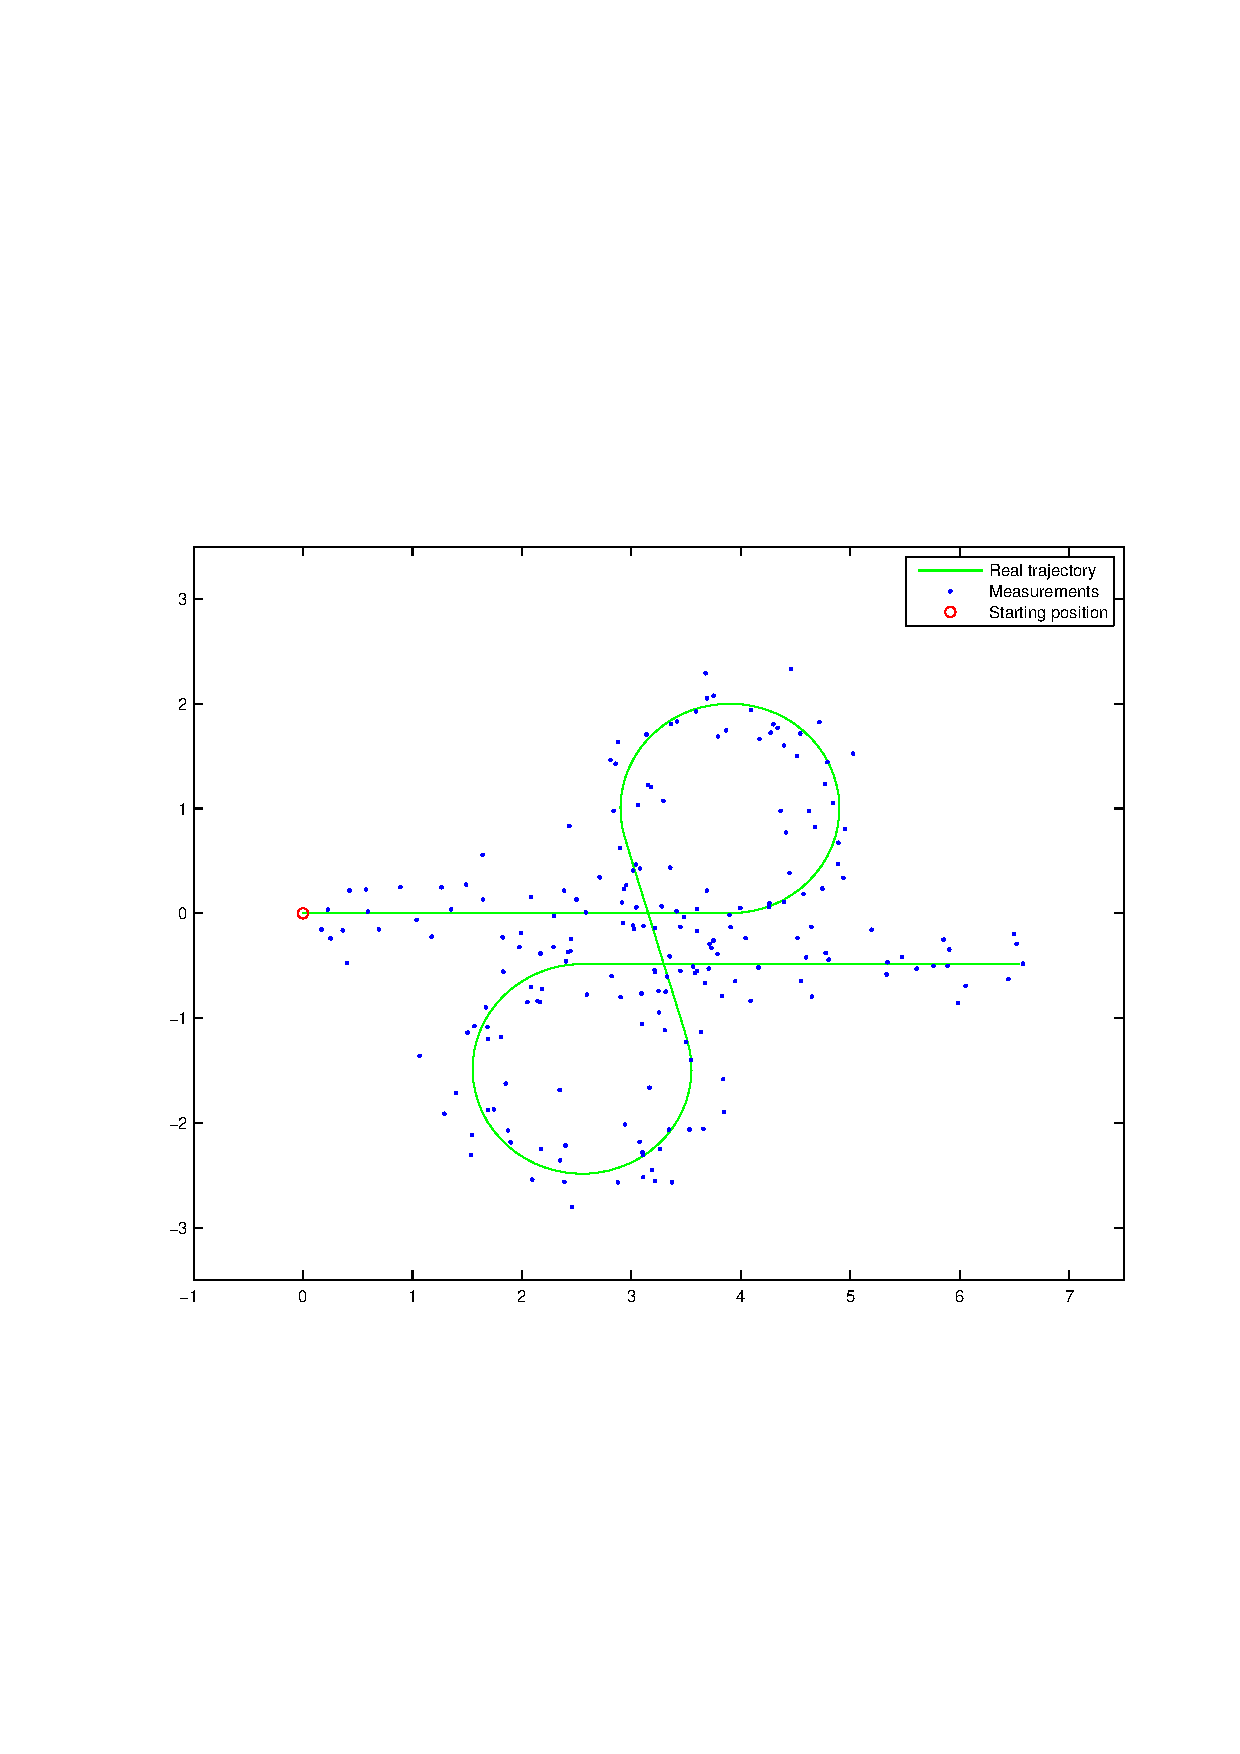
\includegraphics[width=11cm]{pics/eimm1_trajectory}
\caption{ Object's trajectory and a sample of measurements in the
Coordinated turn model demonstration.  }
\label{fig:eimm1_trajectory}
\end{center}
\end{figure}

\begin{figure}
\begin{center}
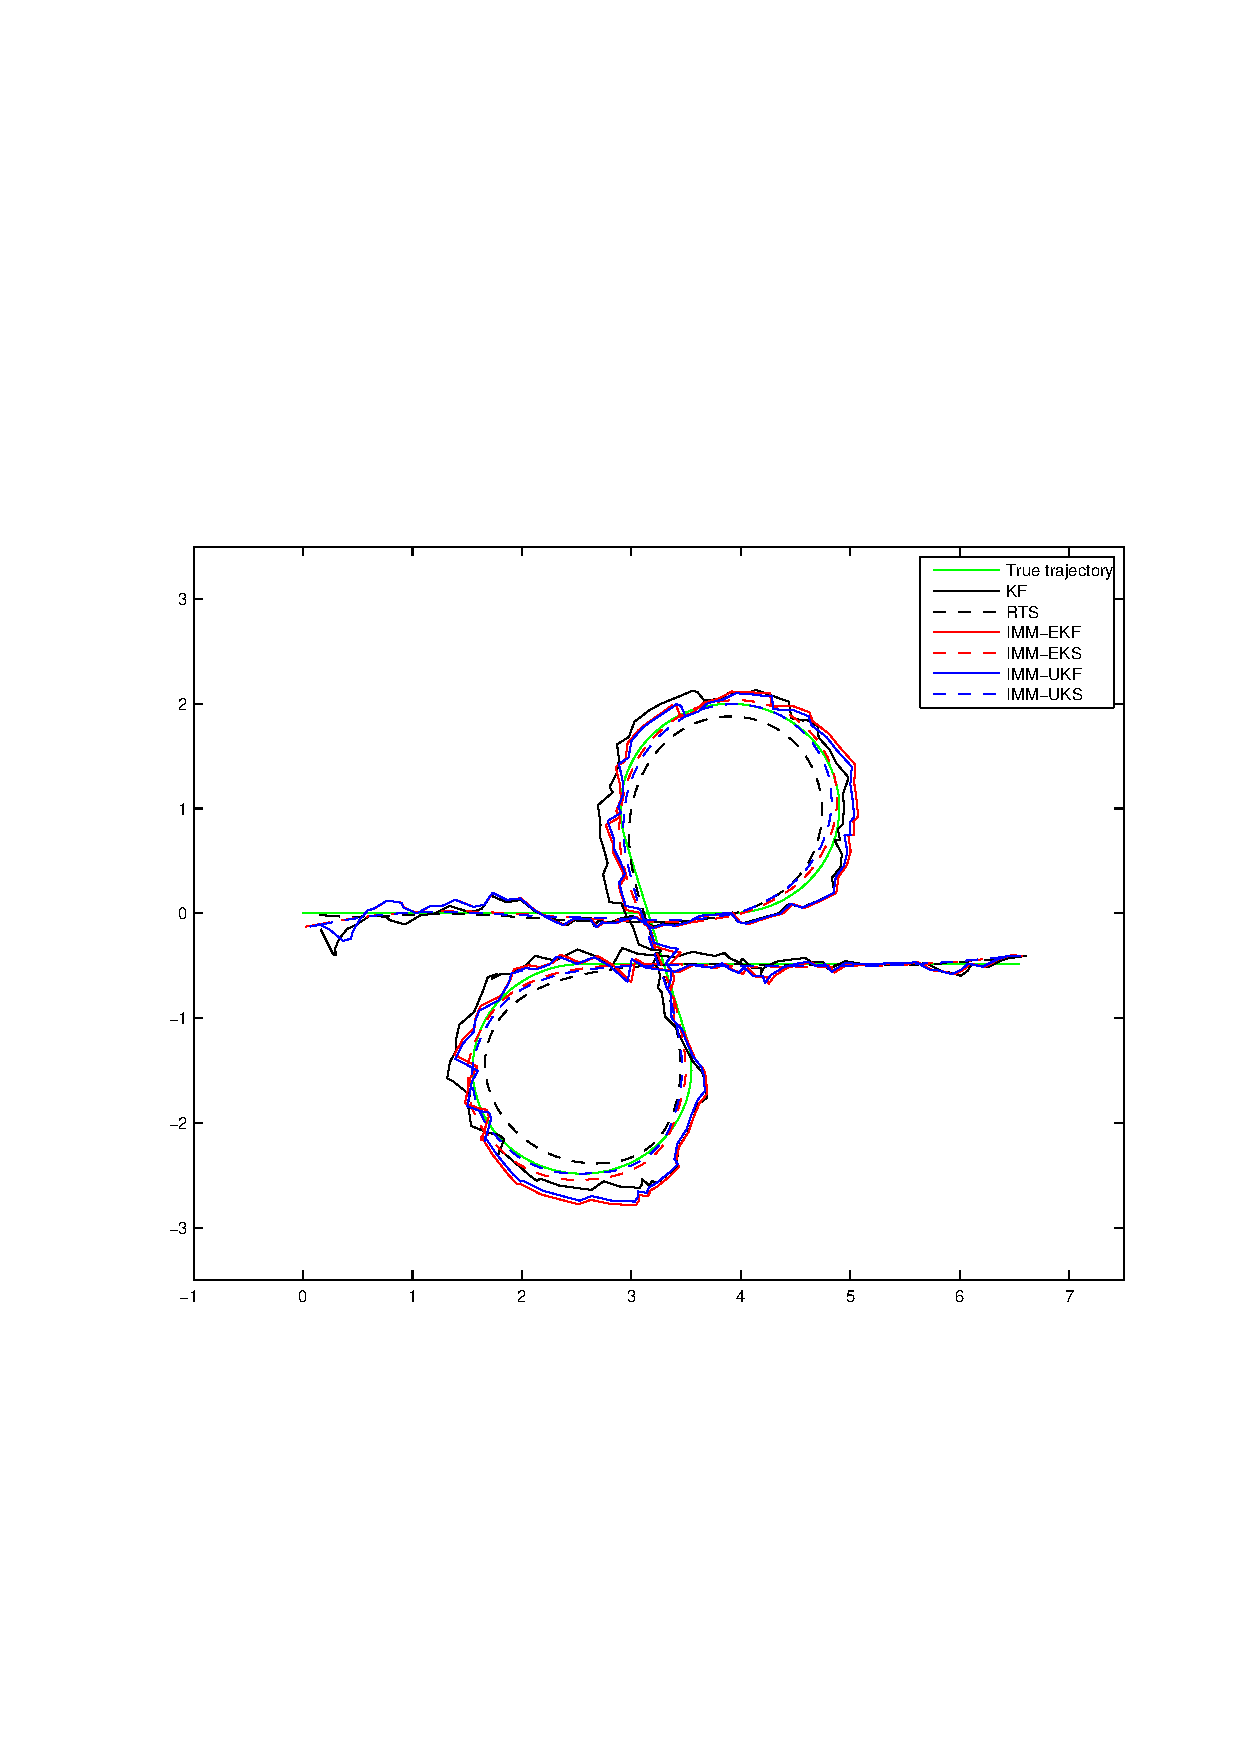
\includegraphics[width=11cm]{pics/eimm1_1}
\caption{ Position estimates in the Coordinated turn model
demonstration.  }
\label{fig:eimm1_1}
\end{center}
\end{figure}

\begin{figure}
\begin{center}
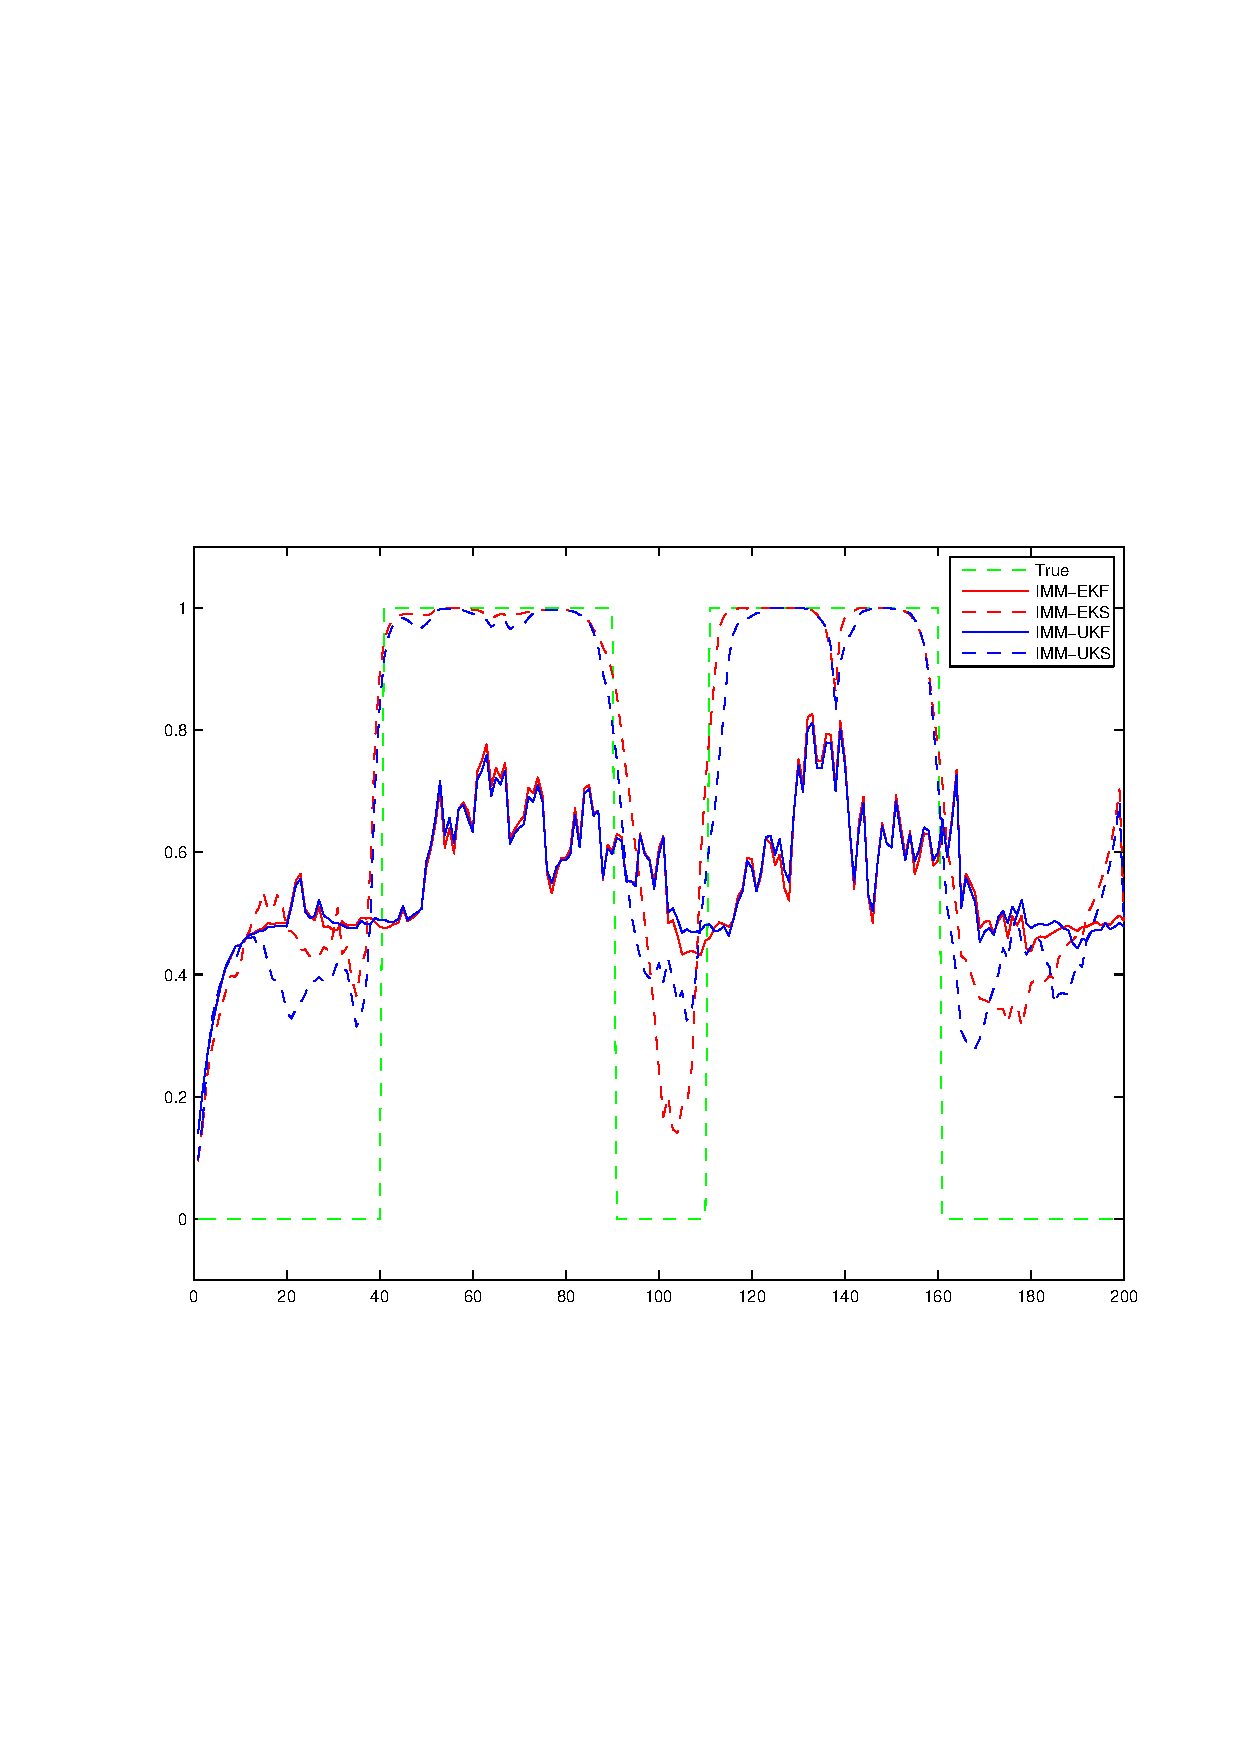
\includegraphics[width=11cm]{pics/eimm1_2}
\caption{ Estimates for model 2's probability in Coordinated turn
model demonstration.  }
\label{fig:eimm1_2}
\end{center}
\end{figure}

\begin{figure}
\begin{center}
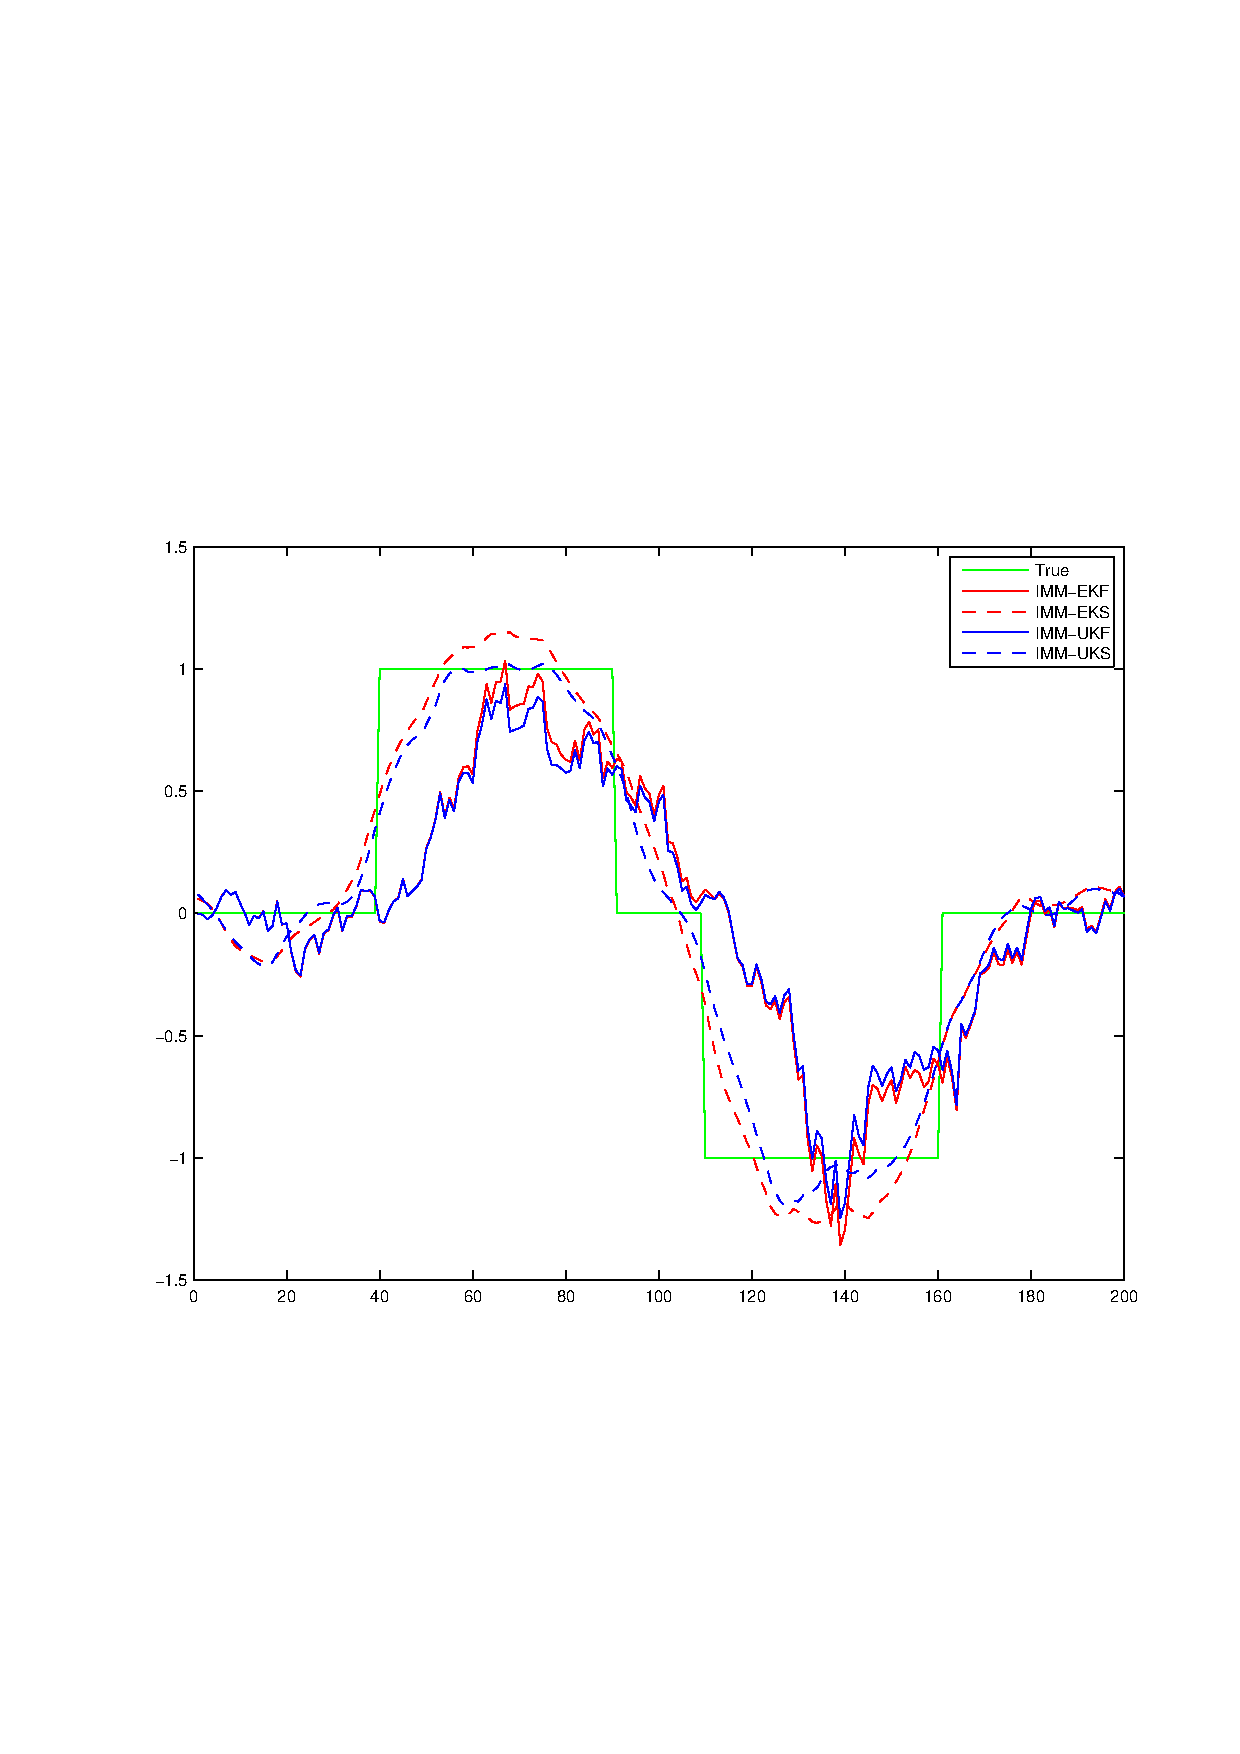
\includegraphics[width=11cm]{pics/eimm1_3}
\caption{ Estimates of the turn rate parameter $\omega_k$ in the
Coordinated turn model demonstration.  }
\label{fig:eimm1_3}
\end{center}
\end{figure}

%  
\begin{table}
\begin{center}
\begin{tabular}{|l|l|} \hline {\it Method}&{\it MSE } \\ \hline KF &
0.0253 \\ KS & 0.0052 \\ EIMM1 & 0.0179 \\ EIMMS1 & 0.0039 \\ UIMM1 &
0.0155 \\ UIMMS1 & 0.0036 \\ \hline
\end{tabular}
\caption{Average MSEs of estimating the position in Tracking Object
with Simple Manouvers example over 100 Monte Carlo runs.}
\label{table:eimm1_mse}
\end{center}
\end{table}
%

\subsection{Demonstration: Bearings Only Tracking of a Manouvering
Target}

We now extend the previous demonstration by replacing the linear
measurement model with a non-linear bearings only measurement model,
which were reviewed in section 2.2.9. The estimation problem is now
harder as we must use a non-linear version of IMM filter update step
in addition to the prediction step, which was used in the previous
demonstration.

The trajectory of the object is exactly the same as in the previous
example. The sensors producing the angle measurements are located in
$(s_x^1,s_y^1) = (-0.5,3.5)$, $(s_x^2,s_y^2) = (-0.5,3.5)$,
$(s_x^3,s_y^3) = (7,-3.5)$ and $(s_x^4,s_y^4) = (7,3.5)$. The
trajectory and the sensor positions are shown in figure
\ref{fig:eimm2_trajectory}.  The standard deviation of the
measurements is set to $\sigma = 0.1$ radians, which is relatively
high.

\begin{figure}
\begin{center}
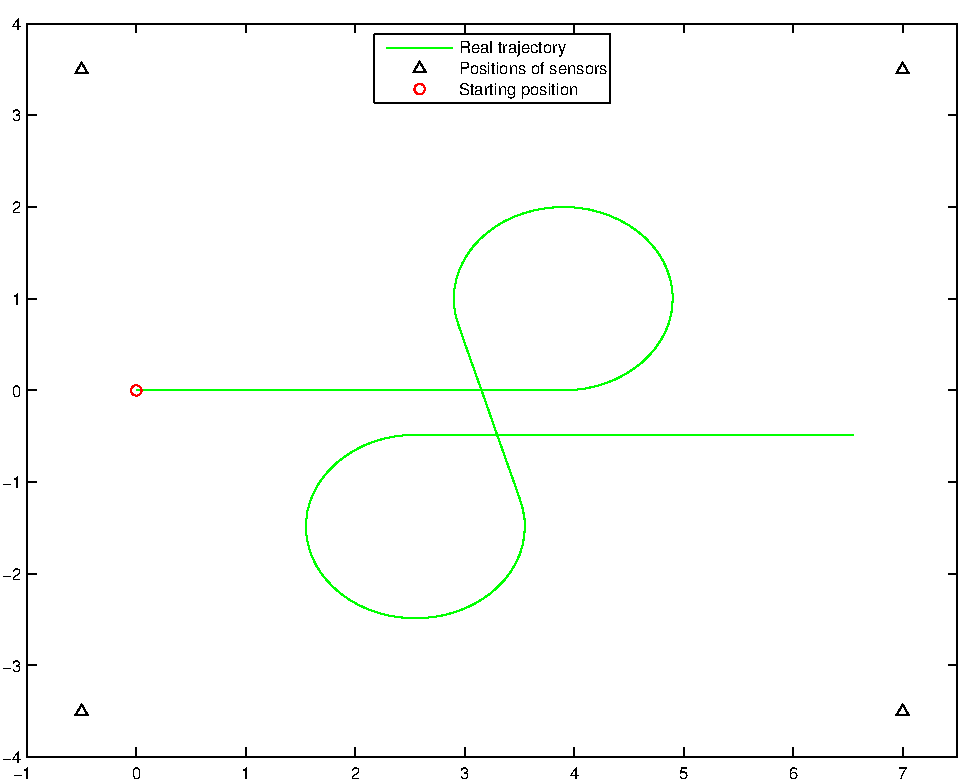
\includegraphics[width=11cm]{pics/eimm2_trajectory}
\caption{ Object's trajectory and positions of the sensors in Bearings
Only Tracking of a Manouvering Target demonstration.  }
\label{fig:eimm2_trajectory}
\end{center}
\end{figure}

The function call of IMM-EKF update step is of form
%
\begin{lstlisting} 
[x_ip,P_ip,mu_ip,m,P] = eimm_update(x_p,P_p,c_j,ind,dims, ...
  Y(:,i),H,h_func,R,h_param);
\end{lstlisting}
%
which differs from the standard IMM filter update with the additional
parameters \texttt{h} and \texttt{h\_param}, which contain the handles
to measurement model functions and their parameters,
respectively. Also, the parameter \texttt{H} now contains the handles
to functions calculating the Jacobian's of the measurement
functions. In IMM-UKF the update function is specified similarly.

The position of the object is estimated with the following methods:
\begin{itemize}
\item EKF and EKS: Extended Kalman filter and (RTS) smoother using the
same Wiener process velocity model as in the previous demonstration in
the case standard Kalman filter.
\item UKF and UKS: Unscented Kalman filter and (RTS) smoother using
the same model as the EKF.
\item IMM-EKF and IMM-EKS: EKF based IMM filter and smoother using the
same combination of Wiener process velocity model and a coordinated
turn model as was used in the previous demonstration in the case of
IMM-EKF and IMM-UKF.
\item IMM-UKF and IMM-UKS: UKF based IMM filter and smoother using the
same models as IMM-EKF.
\end{itemize}
%
A sample of trajectory estimates are plotted in figure
\ref{fig:eimm2_1}. The estimates are clearly more inaccurate than the
ones in the previous section. In figure \ref{fig:eimm2_2} we have
plotted the estimates of model 2's probability for IMM-EKF and
IMM-UKF. The figure look very similar to the one in the previous
demonstration, despite the non-linear and more noisy
measurements. Also the turn rate estimates, which are plotted in
figure \ref{fig:eimm2_3}, are very similar to the ones in the previous
section with exception that now the difference between the smoothed
estimates of IMM-EKF and IMM-UKF is bigger.

\begin{figure}
\begin{center}
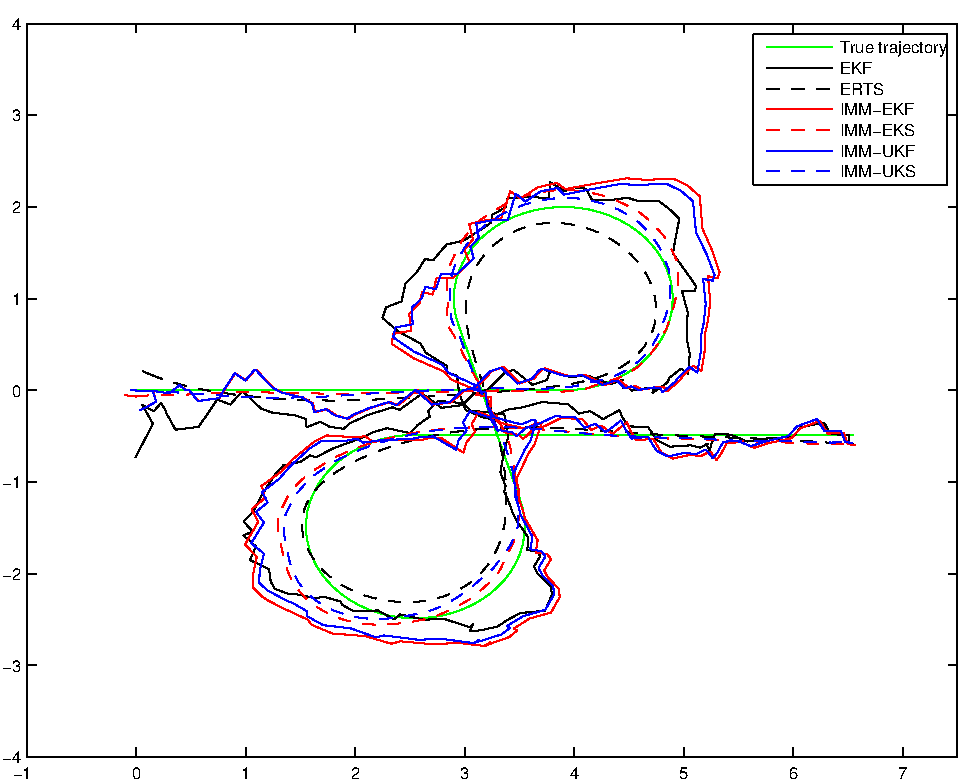
\includegraphics[width=11cm]{pics/eimm2_1}
\caption{ Filtered and smoothed estimates of object's position using
all the tested methods in Bearings Only Tracking of a Manouvering
Target demonstration.  }
\label{fig:eimm2_1}
\end{center}
\end{figure}

\begin{figure}
\begin{center}
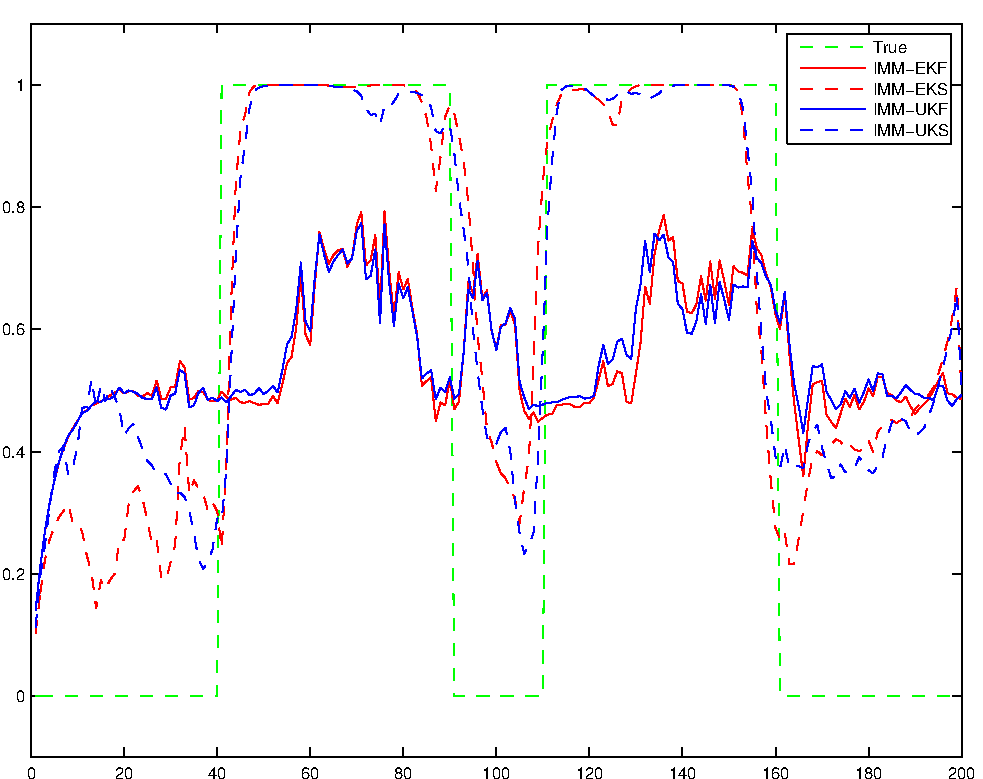
\includegraphics[width=11cm]{pics/eimm2_2}
\caption{ Estimates for model 2's probability in Bearings Only
Tracking of a Manouvering Target demonstration.  }
\label{fig:eimm2_2}
\end{center}
\end{figure}

\begin{figure}
\begin{center}
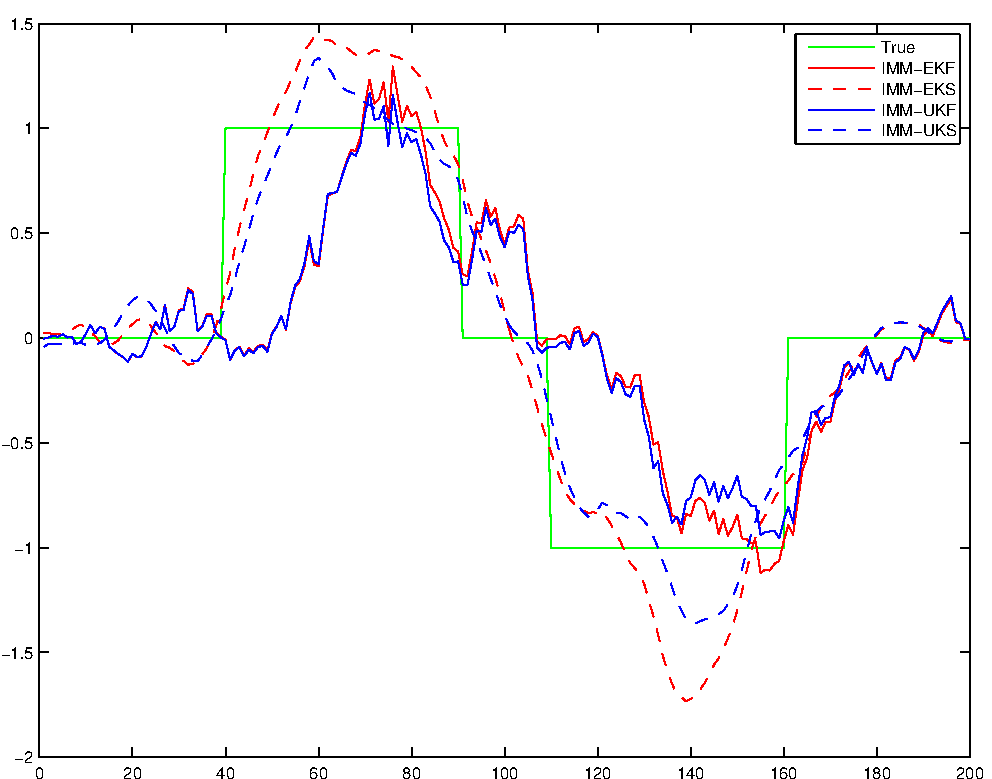
\includegraphics[width=11cm]{pics/eimm2_3}
\caption{ Estimates for the turn rate parameter $\omega_k$ in Bearings
Only Tracking of a Manouvering Target demonstration }
\label{fig:eimm2_3}
\end{center}
\end{figure}

In table \ref{table:eimm_rmse2} we have listed the average mean square
errors of position estimates over 100 Monte Carlo runs.  It can be
observed that the estimates of EKF and UKF are identical in practice,
which is to be expected from Bearings Only Tracking demonstration. The
difference between IMM-UKF and IMM-EKF has grown in the favor of
IMM-UKF, whereas the accuracy of IMM-EKF is now more close to the ones
of EKF and UKF. On the other hand the smoothed estimates of IMM-UKF
and IMM-EKF are still very close to one another, and are considerably
better than the smoothed estimates of EKF and UKF.

%  
\begin{table}
\begin{center}
\begin{tabular}{|l|l|} \hline {\it Method}&{\it MSE } \\ \hline EKF &
0.0606 \\ ERTS & 0.0145 \\ UKF & 0.0609 \\ URTS & 0.0144 \\ IMM-EKF &
0.0544 \\ IMM-EKS & 0.0094 \\ IMM-UKF & 0.0441 \\ IMM-UKS & 0.0089 \\
\hline
\end{tabular}
\caption{Average MSEs of estimating the position in Bearings Only
Tracking of a Manouvering Target example over 100 Monte Carlo runs.}
\label{table:eimm_rmse2}
\end{center}
\end{table}
%

It should be noted that the performance of each tested method could be
tuned by optimizing their parameters (e.g. variance of process noise
of dynamic models, values of model transition matrix in IMM etc.)
more carefully, so the performance differences could change
radically. Still, it is clear that IMM filter does actually work also
with (atleast some) non-linear dynamic and measurement models, and
should be considered as a standard estimation method for multiple
model systems. Also, one should prefer IMM-UKF over IMM-EKF as the
performance is clearly (atleast in these cases) better, and the
implementation is easier, as we have seen in the previous examples.


%
%%%%%%%%%%%%%%%%%%%%%%%%%%%%%%%%%%%%%%%%%%%%%%%%%%%%%%%%%%%%%%%%%%%%%%%%%%%%%%

\clearpage
\newpage





%%%%%%%%%%%%%%%%%%%%%%%%%%%%%%%%%%%%%%%%%%%%%%%%%%%%%%%%%%%%%%%%%%%%%%%%%%%%%%
%
  %%%%%%%%%%%%%%%%%%%%%%%%%%%%%%%%%%%%%%%%%%%%%%%%%%%%%%%%%%%%%%%%%%%%%%%%%%%%%%
%
\chapter{Functions in the Toolbox}
%
%%%%%%%%%%%%%%%%%%%%%%%%%%%%%%%%%%%%%%%%%%%%%%%%%%%%%%%%%%%%%%%%%%%%%%%%%%%%%%

\label{ch:functions}

%% These function reference sheets are automatically generated by a Matlab script.
%% The information shown here is based on the actual function description in 
%% Matlab. Please, if these descriptions contain errors, edit the original
%% function rather than just fixing the problem here.
%%        ~ Arno Solin



\section{Discrete-time State Space Estimation}

\subsection{Linear Kalman Filter}

% This function reference sheet is automatically generated
% by a Matlab script. The information shown here is based on
% the actual function description in Matlab. Please, if this
% description contains errors, edit the original function
% rather than just fixing the problem here.
% --- Script by Arno Solin (Oct 4, 2010)


\subsubsection*{kf\_predict}
\label{function:kf_predict}

\noindent
\begin{tabular*}{\textwidth}{@{\extracolsep{\fill}} | p{0.1\textwidth} p{0.1\textwidth} p{0.7\textwidth} |  }
\hline
\multicolumn{3}{| p{0.9\textwidth} |}{\bf \texttt{kf\_predict}} \\
\multicolumn{3}{| p{0.9\textwidth} |}{
    Perform Kalman Filter prediction step. The model is} \\
\hline
\textbf{Syntax:} & 
  \multicolumn{2}{ p{0.7\textwidth} |}{\texttt{
    [X,P] = KF\_PREDICT(X,P,A,Q,B,U)} } \\
\hline
\multirow{6}{*}{\bf Input:}
 & \texttt{X} & Nx1 mean state estimate of previous step \\
 & \texttt{P} & NxN state covariance of previous step \\
 & \texttt{A} & Transition matrix of discrete model (optional, default identity) \\
 & \texttt{Q} & Process noise of discrete model     (optional, default zero) \\
 & \texttt{B} & Input effect matrix                 (optional, default identity) \\
 & \texttt{U} & Constant input                      (optional, default empty) \\
\hline
\multirow{2}{*}{\bf Output:}
 & \texttt{X} & Predicted state mean \\
 & \texttt{P} & Predicted state covariance
     \\
\hline
\end{tabular*}

% This function reference sheet is automatically generated
% by a Matlab script. The information shown here is based on
% the actual function description in Matlab. Please, if this
% description contains errors, edit the original function
% rather than just fixing the problem here.
% --- Script by Arno Solin (Oct 4, 2010)


\subsubsection*{kf\_update}
\label{function:kf_update}

\noindent
\begin{tabular*}{\textwidth}{@{\extracolsep{\fill}} | p{0.1\textwidth} p{0.1\textwidth} p{0.7\textwidth} |  }
\hline
\multicolumn{3}{| p{0.9\textwidth} |}{\bf \texttt{kf\_update}} \\
\multicolumn{3}{| p{0.9\textwidth} |}{
    Kalman filter measurement update step. Kalman Filter
    model is} \\
\hline
\textbf{Syntax:} & 
  \multicolumn{2}{ p{0.7\textwidth} |}{\texttt{
    [X,P,K,IM,IS,LH] = KF\_UPDATE(X,P,Y,H,R)} } \\
\hline
\multirow{5}{*}{\bf Input:}
 & \texttt{X} & Nx1 mean state estimate after prediction step \\
 & \texttt{P} & NxN state covariance after prediction step \\
 & \texttt{Y} & Dx1 measurement vector. \\
 & \texttt{H} & Measurement matrix. \\
 & \texttt{R} & Measurement noise covariance. \\
\hline
\multirow{6}{*}{\bf Output:}
 & \texttt{X} & Updated state mean \\
 & \texttt{P} & Updated state covariance \\
 & \texttt{K} & Computed Kalman gain \\
 & \texttt{IM} & Mean of predictive distribution of Y \\
 & \texttt{IS} & Covariance or predictive mean of Y \\
 & \texttt{LH} & Predictive probability (likelihood) of measurement.
     \\
\hline
\end{tabular*}

% This function reference sheet is automatically generated
% by a Matlab script. The information shown here is based on
% the actual function description in Matlab. Please, if this
% description contains errors, edit the original function
% rather than just fixing the problem here.
% --- Script by Arno Solin (Oct 4, 2010)


\subsubsection*{kf\_lhood}
\label{function:kf_lhood}

\noindent
\begin{tabular*}{\textwidth}{@{\extracolsep{\fill}} | p{0.1\textwidth} p{0.1\textwidth} p{0.7\textwidth} |  }
\hline
\multicolumn{3}{| p{0.9\textwidth} |}{\bf \texttt{kf\_lhood}} \\
\multicolumn{3}{| p{0.9\textwidth} |}{
    Calculate likelihood of measurement in Kalman filter.
    If and X and P define the parameters of predictive
    distribution (e.g. from KF\_PREDICT)} \\
\hline
\textbf{Syntax:} & 
  \multicolumn{2}{ p{0.7\textwidth} |}{\texttt{
    LH = KF\_LHOOD(X,P,Y,H,R)} } \\
\hline
\multirow{5}{*}{\bf Input:}
 & \texttt{X} & Nx1 state mean \\
 & \texttt{P} & NxN state covariance \\
 & \texttt{Y} & Dx1 measurement vector. \\
 & \texttt{H} & Measurement matrix. \\
 & \texttt{R} & Measurement noise covariance. \\
\hline
\multirow{1}{*}{\bf Output:}
 & \texttt{LH} & Likelihood of measurement.
     \\
\hline
\end{tabular*}

% This function reference sheet is automatically generated
% by a Matlab script. The information shown here is based on
% the actual function description in Matlab. Please, if this
% description contains errors, edit the original function
% rather than just fixing the problem here.
% --- Script by Arno Solin (Oct 4, 2010)


\subsubsection*{kf\_loop}
\label{function:kf_loop}

\noindent
\begin{tabular*}{\textwidth}{@{\extracolsep{\fill}} | p{0.1\textwidth} p{0.1\textwidth} p{0.7\textwidth} |  }
\hline
\multicolumn{3}{| p{0.9\textwidth} |}{\bf \texttt{kf\_loop}} \\
\multicolumn{3}{| p{0.9\textwidth} |}{
     Calculates state estimates for a set measurements using the
     Kalman filter. This function is for convience, as it basically consists
     only of a space reservation for the estimates and of a for-loop which
     calls the predict and update steps of the KF for each time step in
     the measurements.  
   
   See also:
     KF\_PREDICT, KF\_UPDATE
} \\
\hline
\textbf{Syntax:} & 
  \multicolumn{2}{ p{0.7\textwidth} |}{\texttt{
    [MM,PP] = KF\_LOOP(X,P,H,R,Y,A,Q)} } \\
\hline
\multirow{9}{*}{\bf Input:}
 & \texttt{X} & Nx1 initial estimate for the state mean  \\
 & \texttt{P} & NxN initial estimate for the state covariance \\
 & \texttt{H} & DxN measurement matrix \\
 & \texttt{R} & DxD measurement noise covariance \\
 & \texttt{Y} & DxM matrix containing all the measurements. \\
 & \texttt{A} & Transition matrix of the discrete model (optional, default identity) \\
 & \texttt{Q} & Process noise of the discrete model     (optional, default zero)
     \\
 & \texttt{MM} & Filtered state mean sequence \\
 & \texttt{MM} & Filtered state mean sequence \\
\hline
\multirow{2}{*}{\bf Output:}
 & \texttt{MM} & Filtered state mean sequence \\
 & \texttt{PP} & Filtered state covariance sequence
    \\
\hline
\end{tabular*}

% This function reference sheet is automatically generated
% by a Matlab script. The information shown here is based on
% the actual function description in Matlab. Please, if this
% description contains errors, edit the original function
% rather than just fixing the problem here.
% --- Script by Arno Solin (Oct 4, 2010)


\subsubsection*{rts\_smooth}
\label{function:rts_smooth}

\noindent
\begin{tabular*}{\textwidth}{@{\extracolsep{\fill}} | p{0.1\textwidth} p{0.1\textwidth} p{0.7\textwidth} |  }
\hline
\multicolumn{3}{| p{0.9\textwidth} |}{\bf \texttt{rts\_smooth}} \\
\multicolumn{3}{| p{0.9\textwidth} |}{
    Rauch-Tung-Striebel smoother algorithm. Calculate "smoothed"
    sequence from given Kalman filter output sequence
    by conditioning all steps to all measurements.} \\
\hline
\textbf{Syntax:} & 
  \multicolumn{2}{ p{0.7\textwidth} |}{\texttt{
    [M,P,S] = RTS\_SMOOTH(M,P,A,Q)} } \\
\hline
\multirow{4}{*}{\bf Input:}
 & \texttt{M} & NxK matrix of K mean estimates from Kalman filter \\
 & \texttt{P} & NxNxK matrix of K state covariances from Kalman Filter \\
 & \texttt{A} & NxN state transition matrix or NxNxK matrix of K state
        transition matrices for each step. \\
 & \texttt{Q} & NxN process noise covariance matrix or NxNxK matrix
        of K state process noise covariance matrices for each step. \\
\hline
\multirow{3}{*}{\bf Output:}
 & \texttt{M} & Smoothed state mean sequence \\
 & \texttt{P} & Smoothed state covariance sequence \\
 & \texttt{D} & Smoother gain sequence
     \\
\hline
\end{tabular*}

% This function reference sheet is automatically generated
% by a Matlab script. The information shown here is based on
% the actual function description in Matlab. Please, if this
% description contains errors, edit the original function
% rather than just fixing the problem here.
% --- Script by Arno Solin (Oct 4, 2010)


\subsubsection*{tf\_smooth}
\label{function:tf_smooth}

\noindent
\begin{tabular*}{\textwidth}{@{\extracolsep{\fill}} | p{0.1\textwidth} p{0.1\textwidth} p{0.7\textwidth} |  }
\hline
\multicolumn{3}{| p{0.9\textwidth} |}{\bf \texttt{tf\_smooth}} \\
\multicolumn{3}{| p{0.9\textwidth} |}{
    Two filter linear smoother algorithm. Calculate "smoothed"
    sequence from given Kalman filter output sequence
    by conditioning all steps to all measurements.} \\ 
\hline
\textbf{Syntax:} & 
  \multicolumn{2}{ p{0.7\textwidth} |}{\texttt{
    [M,P] = TF\_SMOOTH(M,P,Y,A,Q,H,R, [use\_inf])} } \\
\hline
\multirow{8}{*}{\bf Input:}
 & \texttt{M} & NxK matrix of K mean estimates from Kalman filter \\
 & \texttt{P} & NxNxK matrix of K state covariances from Kalman Filter \\ 
 & \texttt{Y} & Sequence of K measurement as DxK matrix \\
 & \texttt{A} & NxN state transition matrix. \\
 & \texttt{Q} & NxN process noise covariance matrix. \\
 & \texttt{H} & DxN Measurement matrix. \\
 & \texttt{R} & DxD Measurement noise covariance. \\
 & \texttt{use\_inf} & If information filter should be used (default 1) \\
\hline
\multirow{2}{*}{\bf Output:}
 & \texttt{M} & Smoothed state mean sequence \\
 & \texttt{P} & Smoothed state covariance sequence
     \\
\hline
\end{tabular*}





\subsection{Extended Kalman Filter}

% This function reference sheet is automatically generated
% by a Matlab script. The information shown here is based on
% the actual function description in Matlab. Please, if this
% description contains errors, edit the original function
% rather than just fixing the problem here.
% --- Script by Arno Solin (Oct 4, 2010)


\subsubsection*{ekf\_predict1}
\label{function:ekf_predict1}

\noindent
\begin{tabular*}{\textwidth}{@{\extracolsep{\fill}} | p{0.1\textwidth} p{0.1\textwidth} p{0.7\textwidth} |  }
\hline
\multicolumn{3}{| p{0.9\textwidth} |}{\bf \texttt{ekf\_predict1}} \\
\multicolumn{3}{| p{0.9\textwidth} |}{
    Perform Extended Kalman Filter prediction step.} \\
\hline
\textbf{Syntax:} & 
  \multicolumn{2}{ p{0.7\textwidth} |}{\texttt{
    [M,P] = EKF\_PREDICT1(M,P, [A,Q,a,W,param])} } \\
\hline
\multirow{7}{*}{\bf Input:}
 & \texttt{M} & Nx1 mean state estimate of previous step \\
 & \texttt{P} & NxN state covariance of previous step \\
 & \texttt{A} & Derivative of a() with respect to state as
        matrix, inline function, function handle or
        name of function in form A(x,param)       (optional, default eye()) \\
 & \texttt{Q} & Process noise of discrete model               (optional, default zero) \\
 & \texttt{a} & Mean prediction E[a(x[k-1],q=0)] as vector,
        inline function, function handle or name
        of function in form a(x,param)                (optional, default A(x)*X) \\
 & \texttt{W} & Derivative of a() with respect to noise q
        as matrix, inline function, function handle
        or name of function in form W(x,param)        (optional, default identity) \\
 & \texttt{param} & Parameters of a                           (optional, default empty) \\
\hline
\multirow{2}{*}{\bf Output:}
 & \texttt{M} & Updated state mean \\
 & \texttt{P} & Updated state covariance
     \\
\hline
\end{tabular*}

% This function reference sheet is automatically generated
% by a Matlab script. The information shown here is based on
% the actual function description in Matlab. Please, if this
% description contains errors, edit the original function
% rather than just fixing the problem here.
% --- Script by Arno Solin (Oct 4, 2010)


\subsubsection*{ekf\_predict2}
\label{function:ekf_predict2}

\noindent
\begin{tabular*}{\textwidth}{@{\extracolsep{\fill}} | p{0.1\textwidth} p{0.1\textwidth} p{0.7\textwidth} |  }
\hline
\multicolumn{3}{| p{0.9\textwidth} |}{\bf \texttt{ekf\_predict2}} \\
\multicolumn{3}{| p{0.9\textwidth} |}{
    Perform Extended Kalman Filter prediction step.} \\
\hline
\textbf{Syntax:} & 
  \multicolumn{2}{ p{0.7\textwidth} |}{\texttt{
    [M,P] = EKF\_PREDICT2(M,P, [A,F,Q,a,W,param])} } \\
\hline
\multirow{8}{*}{\bf Input:}
 & \texttt{M} & Nx1 mean state estimate of previous step \\
 & \texttt{P} & NxN state covariance of previous step \\
 & \texttt{A} & Derivative of a() with respect to state as
        matrix, inline function, function handle or
        name of function in form A(x,param)                 (optional, default identity) \\
 & \texttt{F} & NxNxN Hessian matrix of the state transition function
        w.r.t. state variables as matrix, inline
        function, function handle or name of function
        in form F(x,param)                                  (optional, default identity) \\
 & \texttt{Q} & Process noise of discrete model                     (optional, default zero) \\
 & \texttt{a} & Mean prediction E[a(x[k-1],q=0)] as vector,
        inline function, function handle or name
        of function in form a(x,param)                      (optional, default A(x)*X) \\
 & \texttt{W} & Derivative of a() with respect to noise q
        as matrix, inline function, function handle
        or name of function in form W(x,k-1,param)          (optional, default identity) \\
 & \texttt{param} & Parameters of a                                 (optional, default empty) \\
\hline
\multirow{2}{*}{\bf Output:}
 & \texttt{M} & Updated state mean \\
 & \texttt{P} & Updated state covariance
     \\
\hline
\end{tabular*}

% This function reference sheet is automatically generated
% by a Matlab script. The information shown here is based on
% the actual function description in Matlab. Please, if this
% description contains errors, edit the original function
% rather than just fixing the problem here.
% --- Script by Arno Solin (Oct 4, 2010)


\subsubsection*{ekf\_update1}
\label{function:ekf_update1}

\noindent
\begin{tabular*}{\textwidth}{@{\extracolsep{\fill}} | p{0.1\textwidth} p{0.1\textwidth} p{0.7\textwidth} |  }
\hline
\multicolumn{3}{| p{0.9\textwidth} |}{\bf \texttt{ekf\_update1}} \\
\multicolumn{3}{| p{0.9\textwidth} |}{
    Extended Kalman Filter measurement update step.
    EKF model is} \\
\hline
\textbf{Syntax:} & 
  \multicolumn{2}{ p{0.7\textwidth} |}{\texttt{
    [M,P,K,MU,S,LH] = EKF\_UPDATE1(M,P,Y,H,R, [h,V,param])} } \\
\hline
\multirow{8}{*}{\bf Input:}
 & \texttt{M} & Nx1 mean state estimate after prediction step \\
 & \texttt{P} & NxN state covariance after prediction step \\
 & \texttt{Y} & Dx1 measurement vector. \\
 & \texttt{H} & Derivative of h() with respect to state as matrix,
         inline function, function handle or name
         of function in form H(x,param) \\
 & \texttt{R} & Measurement noise covariance. \\
 & \texttt{h} & Mean prediction (innovation) as vector,
         inline function, function handle or name
         of function in form h(x,param).               (optional, default H(x)*X) \\
 & \texttt{V} & Derivative of h() with respect to noise as matrix,
         inline function, function handle or name
         of function in form V(x,param).               (optional, default identity) \\
 & \texttt{param} & Parameters of h                            (optional, default empty) \\
\hline
\multirow{6}{*}{\bf Output:}
 & \texttt{M} & Updated state mean \\
 & \texttt{P} & Updated state covariance \\
 & \texttt{K} & Computed Kalman gain \\
 & \texttt{MU} & Predictive mean of Y \\
 & \texttt{S} & Predictive covariance of Y \\
 & \texttt{LH} & Predictive probability (likelihood) of measurement.
     \\
\hline
\end{tabular*}

% This function reference sheet is automatically generated
% by a Matlab script. The information shown here is based on
% the actual function description in Matlab. Please, if this
% description contains errors, edit the original function
% rather than just fixing the problem here.
% --- Script by Arno Solin (Oct 4, 2010)


\subsubsection*{ekf\_update2}
\label{function:ekf_update2}

\noindent
\begin{tabular*}{\textwidth}{@{\extracolsep{\fill}} | p{0.1\textwidth} p{0.1\textwidth} p{0.7\textwidth} |  }
\hline
\multicolumn{3}{| p{0.9\textwidth} |}{\bf \texttt{ekf\_update2}} \\
\multicolumn{3}{| p{0.9\textwidth} |}{
    Extended Kalman Filter measurement update step.
    EKF model is} \\
\hline
\textbf{Syntax:} & 
  \multicolumn{2}{ p{0.7\textwidth} |}{\texttt{
    [M,P,K,MU,S,LH] = EKF\_UPDATE2(M,P,Y,H,H\_xx,R, [h,V,param])} } \\
\hline
\multirow{9}{*}{\bf Input:}
 & \texttt{M} & Nx1 mean state estimate after prediction step \\
 & \texttt{P} & NxN state covariance after prediction step \\
 & \texttt{Y} & Dx1 measurement vector. \\
 & \texttt{H} & Derivative of h() with respect to state as matrix,
         inline function, function handle or name
         of function in form H(x,param) \\
 & \texttt{H\_xx} & DxNxN Hessian of h() with respect to state as matrix,
           inline function, function handle or name of function
           in form H\_xx(x,param)  \\
 & \texttt{R} & Measurement noise covariance. \\
 & \texttt{h} & Mean prediction (measurement model) as vector,
         inline function, function handle or name
         of function in form h(x,param).                 (optional, default H(x)*X) \\
 & \texttt{V} & Derivative of h() with respect to noise as matrix,
         inline function, function handle or name
         of function in form V(x,param).                 (optional, default identity) \\
 & \texttt{param} & Parameters of h                              (optional, default empty) \\
\hline
\multirow{6}{*}{\bf Output:}
 & \texttt{M} & Updated state mean \\
 & \texttt{P} & Updated state covariance \\
 & \texttt{K} & Computed Kalman gain \\
 & \texttt{MU} & Predictive mean of Y \\
 & \texttt{S} & Predictive covariance Y \\
 & \texttt{LH} & Predictive probability (likelihood) of measurement.
     \\
\hline
\end{tabular*}

% This function reference sheet is automatically generated
% by a Matlab script. The information shown here is based on
% the actual function description in Matlab. Please, if this
% description contains errors, edit the original function
% rather than just fixing the problem here.
% --- Script by Arno Solin (Oct 4, 2010)


\subsubsection*{erts\_smooth1}
\label{function:erts_smooth1}

\noindent
\begin{tabular*}{\textwidth}{@{\extracolsep{\fill}} | p{0.1\textwidth} p{0.1\textwidth} p{0.7\textwidth} |  }
\hline
\multicolumn{3}{| p{0.9\textwidth} |}{\bf \texttt{erts\_smooth1}} \\
\multicolumn{3}{| p{0.9\textwidth} |}{
    Extended Rauch-Tung-Striebel smoother algorithm. Calculate
    "smoothed" sequence from given Kalman filter output sequence by
    conditioning all steps to all measurements.} \\
\hline
\textbf{Syntax:} & 
  \multicolumn{2}{ p{0.7\textwidth} |}{\texttt{
    [M,P,D] = ERTS\_SMOOTH1(M,P,A,Q, [a,W,param,same\_p])} } \\
\hline
\multirow{8}{*}{\bf Input:}
 & \texttt{M} & NxK matrix of K mean estimates from Unscented Kalman filter \\
 & \texttt{P} & NxNxK matrix of K state covariances from Unscented Kalman Filter \\
 & \texttt{A} & Derivative of a() with respect to state as
        matrix, inline function, function handle or
        name of function in form A(x,param)                 (optional, default eye()) \\
 & \texttt{Q} & Process noise of discrete model                       (optional, default zero) \\
 & \texttt{a} & Mean prediction E[a(x[k-1],q=0)] as vector,
        inline function, function handle or name
        of function in form a(x,param)                        (optional, default A(x)*X) \\
 & \texttt{W} & Derivative of a() with respect to noise q
        as matrix, inline function, function handle
        or name of function in form W(x,param)                (optional, default identity) \\
 & \texttt{param} & Parameters of a. Parameters should be a single cell array, vector or a matrix
            containing the same parameters for each step or if different parameters
            are used on each step they must be a cell array of the format
            \{ param\_1, param\_2, ...\}, where param\_x contains the parameters for
            step x as a cell array, a vector or a matrix.     (optional, default empty) \\
 & \texttt{same\_p} & 1 if the same parameters should be
             used on every time step                          (optional, default 1)
                                    
                           \\
\hline
\multirow{3}{*}{\bf Output:}
 & \texttt{K} & Smoothed state mean sequence \\
 & \texttt{P} & Smoothed state covariance sequence \\
 & \texttt{D} & Smoother gain sequence
     \\
\hline
\end{tabular*}

% This function reference sheet is automatically generated
% by a Matlab script. The information shown here is based on
% the actual function description in Matlab. Please, if this
% description contains errors, edit the original function
% rather than just fixing the problem here.
% --- Script by Arno Solin (Oct 4, 2010)


\subsubsection*{etf\_smooth1}
\label{function:etf_smooth1}

\noindent
\begin{tabular*}{\textwidth}{@{\extracolsep{\fill}} | p{0.1\textwidth} p{0.1\textwidth} p{0.7\textwidth} |  }
\hline
\multicolumn{3}{| p{0.9\textwidth} |}{\bf \texttt{etf\_smooth1}} \\
\multicolumn{3}{| p{0.9\textwidth} |}{
    Two filter nonlinear smoother algorithm. Calculate "smoothed"
    sequence from given extended Kalman filter output sequence
    by conditioning all steps to all measurements.} \\
\hline
\textbf{Syntax:} & 
  \multicolumn{2}{ p{0.7\textwidth} |}{\texttt{
    [M,P] = ETF\_SMOOTH1(M,P,Y,A,Q,ia,W,aparam, H,R,h,V,hparam,same\_p\_a,same\_p\_h)} } \\
\hline
\multirow{15}{*}{\bf Input:}
 & \texttt{M} & NxK matrix of K mean estimates from Kalman filter \\
 & \texttt{P} & NxNxK matrix of K state covariances from Kalman Filter \\
 & \texttt{Y} & Measurement vector \\
 & \texttt{A} & Derivative of a() with respect to state as
        matrix, inline function, function handle or
        name of function in form A(x,param)       (optional, default eye()) \\
 & \texttt{Q} & Process noise of discrete model           (optional, default zero) \\
 & \texttt{ia} & Inverse prediction function as vector,
        inline function, function handle or name
        of function in form ia(x,param)           (optional, default inv(A(x))*X) \\
 & \texttt{W} & Derivative of a() with respect to noise q
        as matrix, inline function, function handle
        or name of function in form W(x,param)    (optional, default identity) \\
 & \texttt{aparam} & Parameters of a. Parameters should be a single cell array, vector or a matrix
            containing the same parameters for each step or if different parameters
            are used on each step they must be a cell array of the format
            \{ param\_1, param\_2, ...\}, where param\_x contains the parameters for
            step x as a cell array, a vector or a matrix.   (optional, default empty) \\
 & \texttt{H} & Derivative of h() with respect to state as matrix,
         inline function, function handle or name
         of function in form H(x,param) \\
 & \texttt{R} & Measurement noise covariance. \\
 & \texttt{h} & Mean prediction (measurement model) as vector,
         inline function, function handle or name
         of function in form h(x,param).  (optional, default H(x)*X) \\
 & \texttt{V} & Derivative of h() with respect to noise as matrix,
         inline function, function handle or name
         of function in form V(x,param).  (optional, default identity) \\
 & \texttt{hparam} & Parameters of h. See the description of aparam for the format of
              parameters.                  (optional, default aparam) \\
 & \texttt{same\_p\_a} & If 1 uses the same parameters 
               on every time step for a    (optional, default 1)  \\
 & \texttt{same\_p\_h} & If 1 uses the same parameters 
               on every time step for h    (optional, default 1)  \\
\hline
\multirow{2}{*}{\bf Output:}
 & \texttt{M} & Smoothed state mean sequence \\
 & \texttt{P} & Smoothed state covariance sequence
     \\
\hline
\end{tabular*}



\subsection{Unscented Kalman filter}

% This function reference sheet is automatically generated
% by a Matlab script. The information shown here is based on
% the actual function description in Matlab. Please, if this
% description contains errors, edit the original function
% rather than just fixing the problem here.
% --- Script by Arno Solin (Oct 4, 2010)


\subsubsection*{ukf\_predict1}
\label{function:ukf_predict1}

\noindent
\begin{tabular*}{\textwidth}{@{\extracolsep{\fill}} | p{0.1\textwidth} p{0.1\textwidth} p{0.7\textwidth} |  }
\hline
\multicolumn{3}{| p{0.9\textwidth} |}{\bf \texttt{ukf\_predict1}} \\
\multicolumn{3}{| p{0.9\textwidth} |}{
    Perform additive form Unscented Kalman Filter prediction step.} \\
\hline
\textbf{Syntax:} & 
  \multicolumn{2}{ p{0.7\textwidth} |}{\texttt{
    [M,P] = UKF\_PREDICT1(M,P, [a,Q,param,alpha,beta,kappa,mat])} } \\
\hline
\multirow{9}{*}{\bf Input:}
 & \texttt{M} & Nx1 mean state estimate of previous step \\
 & \texttt{P} & NxN state covariance of previous step \\
 & \texttt{a} & Dynamic model function as a matrix A defining
        linear function a(x) = A*x, inline function,
        function handle or name of function in
        form a(x,param)                   (optional, default eye()) \\
 & \texttt{Q} & Process noise of discrete model   (optional, default zero) \\
 & \texttt{param} & Parameters of a               (optional, default empty) \\
 & \texttt{alpha} & Transformation parameter      (optional) \\
 & \texttt{beta} & Transformation parameter      (optional) \\
 & \texttt{kappa} & Transformation parameter      (optional) \\
 & \texttt{mat} & If 1 uses matrix form         (optional, default 0) \\
\hline
\multirow{2}{*}{\bf Output:}
 & \texttt{M} & Updated state mean \\
 & \texttt{P} & Updated state covariance \\
\hline
\end{tabular*}

% This function reference sheet is automatically generated
% by a Matlab script. The information shown here is based on
% the actual function description in Matlab. Please, if this
% description contains errors, edit the original function
% rather than just fixing the problem here.
% --- Script by Arno Solin (Oct 4, 2010)


\subsubsection*{ukf\_predict2}
\label{function:ukf_predict2}

\noindent
\begin{tabular*}{\textwidth}{@{\extracolsep{\fill}} | p{0.1\textwidth} p{0.1\textwidth} p{0.7\textwidth} |  }
\hline
\multicolumn{3}{| p{0.9\textwidth} |}{\bf \texttt{ukf\_predict2}} \\
\multicolumn{3}{| p{0.9\textwidth} |}{
    Perform augmented form Unscented Kalman Filter prediction step
    for model} \\
\hline
\textbf{Syntax:} & 
  \multicolumn{2}{ p{0.7\textwidth} |}{\texttt{
    [M,P] = UKF\_PREDICT2(M,P,a,Q, [param,alpha,beta,kappa])} } \\
\hline
\multirow{9}{*}{\bf Input:}
 & \texttt{M} & Nx1 mean state estimate of previous step \\
 & \texttt{P} & NxN state covariance of previous step \\
 & \texttt{a} & Dynamic model function as inline function,
        function handle or name of function in
        form a([x;w],param) \\
 & \texttt{Q} & Non-singular covariance of process noise w \\
 & \texttt{param} & Parameters of a               (optional, default empty) \\
 & \texttt{alpha} & Transformation parameter      (optional) \\
 & \texttt{beta} & Transformation parameter      (optional) \\
 & \texttt{kappa} & Transformation parameter      (optional) \\
 & \texttt{mat} & If 1 uses matrix form         (optional, default 0) \\
\hline
\multirow{2}{*}{\bf Output:}
 & \texttt{M} & Updated state mean \\
 & \texttt{P} & Updated state covariance \\
\hline
\end{tabular*}

% This function reference sheet is automatically generated
% by a Matlab script. The information shown here is based on
% the actual function description in Matlab. Please, if this
% description contains errors, edit the original function
% rather than just fixing the problem here.
% --- Script by Arno Solin (Oct 4, 2010)


\subsubsection*{ukf\_predict3}
\label{function:ukf_predict3}

\noindent
\begin{tabular*}{\textwidth}{@{\extracolsep{\fill}} | p{0.1\textwidth} p{0.1\textwidth} p{0.7\textwidth} |  }
\hline
\multicolumn{3}{| p{0.9\textwidth} |}{\bf \texttt{ukf\_predict3}} \\
\multicolumn{3}{| p{0.9\textwidth} |}{
    Perform augmented form Unscented Kalman Filter prediction step
    for model} \\
\hline
\textbf{Syntax:} & 
  \multicolumn{2}{ p{0.7\textwidth} |}{\texttt{
    [M,P,X,w] = UKF\_PREDICT3(M,P,a,Q,R, [param,alpha,beta,kappa])} } \\
\hline
\multirow{10}{*}{\bf Input:}
 & \texttt{M} & Nx1 mean state estimate of previous step \\
 & \texttt{P} & NxN state covariance of previous step \\
 & \texttt{a} & Dynamic model function as inline function,
        function handle or name of function in
        form a([x;w],param) \\
 & \texttt{Q} & Non-singular covariance of process noise w \\
 & \texttt{R} & Measurement covariance. \\
 & \texttt{param} & Parameters of a               (optional, default empty) \\
 & \texttt{alpha} & Transformation parameter      (optional) \\
 & \texttt{beta} & Transformation parameter      (optional) \\
 & \texttt{kappa} & Transformation parameter      (optional) \\
 & \texttt{mat} & If 1 uses matrix form         (optional, default 0) \\
\hline
\multirow{4}{*}{\bf Output:}
 & \texttt{M} & Updated state mean \\
 & \texttt{P} & Updated state covariance \\
 & \texttt{X} & Sigma points of x \\
 & \texttt{w} & Weights as cell array \{mean-weights,cov-weights,c\} \\
\hline
\end{tabular*}

% This function reference sheet is automatically generated
% by a Matlab script. The information shown here is based on
% the actual function description in Matlab. Please, if this
% description contains errors, edit the original function
% rather than just fixing the problem here.
% --- Script by Arno Solin (Oct 4, 2010)


\subsubsection*{ukf\_update1}
\label{function:ukf_update1}

\noindent
\begin{tabular*}{\textwidth}{@{\extracolsep{\fill}} | p{0.1\textwidth} p{0.1\textwidth} p{0.7\textwidth} |  }
\hline
\multicolumn{3}{| p{0.9\textwidth} |}{\bf \texttt{ukf\_update1}} \\
\multicolumn{3}{| p{0.9\textwidth} |}{
    Perform additive form Discrete Unscented Kalman Filter (UKF)
    measurement update step. Assumes additive measurement
    noise.} \\
\hline
\textbf{Syntax:} & 
  \multicolumn{2}{ p{0.7\textwidth} |}{\texttt{
    [M,P,K,MU,S,LH] = UKF\_UPDATE1(M,P,Y,h,R,param, alpha,beta,kappa,mat)} } \\
\hline
\multirow{10}{*}{\bf Input:}
 & \texttt{M} & Mean state estimate after prediction step \\
 & \texttt{P} & State covariance after prediction step \\
 & \texttt{Y} & Measurement vector. \\
 & \texttt{h} & Measurement model function as a matrix H defining
         linear function h(x) = H*x, inline function,
         function handle or name of function in
         form h(x,param) \\
 & \texttt{R} & Measurement covariance. \\
 & \texttt{param} & Parameters of a               (optional, default empty) \\
 & \texttt{alpha} & Transformation parameter      (optional) \\
 & \texttt{beta} & Transformation parameter      (optional) \\
 & \texttt{kappa} & Transformation parameter      (optional) \\
 & \texttt{mat} & If 1 uses matrix form         (optional, default 0) \\
\hline
\multirow{6}{*}{\bf Output:}
 & \texttt{M} & Updated state mean \\
 & \texttt{P} & Updated state covariance \\
 & \texttt{K} & Computed Kalman gain \\
 & \texttt{MU} & Predictive mean of Y \\
 & \texttt{S} & Predictive covariance Y \\
 & \texttt{LH} & Predictive probability (likelihood) of measurement.
     \\
\hline
\end{tabular*}


% This function reference sheet is automatically generated
% by a Matlab script. The information shown here is based on
% the actual function description in Matlab. Please, if this
% description contains errors, edit the original function
% rather than just fixing the problem here.
% --- Script by Arno Solin (Oct 4, 2010)


\subsubsection*{ukf\_update2}
\label{function:ukf_update2}

\noindent
\begin{tabular*}{\textwidth}{@{\extracolsep{\fill}} | p{0.1\textwidth} p{0.1\textwidth} p{0.7\textwidth} |  }
\hline
\multicolumn{3}{| p{0.9\textwidth} |}{\bf \texttt{ukf\_update2}} \\
\multicolumn{3}{| p{0.9\textwidth} |}{
    Perform augmented form Discrete Unscented Kalman Filter (UKF)
    measurement update step. Assumes additive measurement
    noise.} \\
\hline
\textbf{Syntax:} & 
  \multicolumn{2}{ p{0.7\textwidth} |}{\texttt{
    [M,P,K,MU,IS,LH] = UKF\_UPDATE2(M,P,Y,h,R,param, alpha,beta,kappa,mat)} } \\
\hline
\multirow{10}{*}{\bf Input:}
 & \texttt{M} & Mean state estimate after prediction step \\
 & \texttt{P} & State covariance after prediction step \\
 & \texttt{Y} & Measurement vector. \\
 & \texttt{h} & Measurement model function as a matrix H defining
         linear function h(x) = H*x+r, inline function,
         function handle or name of function in
         form h([x;r],param) \\
 & \texttt{R} & Measurement covariance. \\
 & \texttt{param} & Parameters of a               (optional, default empty) \\
 & \texttt{alpha} & Transformation parameter      (optional) \\
 & \texttt{beta} & Transformation parameter      (optional) \\
 & \texttt{kappa} & Transformation parameter      (optional) \\
 & \texttt{mat} & If 1 uses matrix form         (optional, default 0) \\
\hline
\multirow{6}{*}{\bf Output:}
 & \texttt{M} & Updated state mean \\
 & \texttt{P} & Updated state covariance \\
 & \texttt{K} & Computed Kalman gain \\
 & \texttt{MU} & Predictive mean of Y \\
 & \texttt{S} & Predictive covariance Y \\
 & \texttt{LH} & Predictive probability (likelihood) of measurement.
     \\
\hline
\end{tabular*}


% This function reference sheet is automatically generated
% by a Matlab script. The information shown here is based on
% the actual function description in Matlab. Please, if this
% description contains errors, edit the original function
% rather than just fixing the problem here.
% --- Script by Arno Solin (Oct 4, 2010)


\subsubsection*{ukf\_update3}
\label{function:ukf_update3}

\noindent
\begin{tabular*}{\textwidth}{@{\extracolsep{\fill}} | p{0.1\textwidth} p{0.1\textwidth} p{0.7\textwidth} |  }
\hline
\multicolumn{3}{| p{0.9\textwidth} |}{\bf \texttt{ukf\_update3}} \\
\multicolumn{3}{| p{0.9\textwidth} |}{
    Perform augmented form Discrete Unscented Kalman Filter (UKF)
    measurement update step. Assumes additive measurement
    noise.} \\
\hline
\textbf{Syntax:} & 
  \multicolumn{2}{ p{0.7\textwidth} |}{\texttt{
    [M,P,K,MU,IS,LH] = UKF\_UPDATE3(M,P,Y,h,R,X,w,param, alpha,beta,kappa,mat,sigmas)} } \\
\hline
\multirow{12}{*}{\bf Input:}
 & \texttt{M} & Mean state estimate after prediction step \\
 & \texttt{P} & State covariance after prediction step \\
 & \texttt{Y} & Measurement vector. \\
 & \texttt{h} & Measurement model function as a matrix H defining
         linear function h(x) = H*x+r, inline function,
         function handle or name of function in
         form h([x;r],param) \\
 & \texttt{R} & Measurement covariance. \\
 & \texttt{X} & Sigma points of x \\
 & \texttt{w} & Weights as cell array \{mean-weights,cov-weights,c\} \\
 & \texttt{param} & Parameters of a               (optional, default empty) \\
 & \texttt{alpha} & Transformation parameter      (optional) \\
 & \texttt{beta} & Transformation parameter      (optional) \\
 & \texttt{kappa} & Transformation parameter      (optional) \\
 & \texttt{mat} & If 1 uses matrix form         (optional, default 0) \\
\hline
\multirow{6}{*}{\bf Output:}
 & \texttt{M} & Updated state mean \\
 & \texttt{P} & Updated state covariance \\
 & \texttt{K} & Computed Kalman gain \\
 & \texttt{MU} & Predictive mean of Y \\
 & \texttt{S} & Predictive covariance Y \\
 & \texttt{LH} & Predictive probability (likelihood) of measurement.
     \\
\hline
\end{tabular*}


% This function reference sheet is automatically generated
% by a Matlab script. The information shown here is based on
% the actual function description in Matlab. Please, if this
% description contains errors, edit the original function
% rather than just fixing the problem here.
% --- Script by Arno Solin (Oct 4, 2010)


\subsubsection*{urts\_smooth1}
\label{function:urts_smooth1}

\noindent
\begin{tabular*}{\textwidth}{@{\extracolsep{\fill}} | p{0.1\textwidth} p{0.1\textwidth} p{0.7\textwidth} |  }
\hline
\multicolumn{3}{| p{0.9\textwidth} |}{\bf \texttt{urts\_smooth1}} \\
\multicolumn{3}{| p{0.9\textwidth} |}{} \\
\hline
\textbf{Syntax:} & 
  \multicolumn{2}{ p{0.7\textwidth} |}{\texttt{
    [M,P,D] = URTS\_SMOOTH1(M,P,a,Q, [param,alpha,beta,kappa,mat,same\_p])} } \\
\hline
\multirow{10}{*}{\bf Input:}
 & \texttt{M} & NxK matrix of K mean estimates from Unscented Kalman filter \\
 & \texttt{P} & NxNxK matrix of K state covariances from Unscented Kalman Filter \\
 & \texttt{a} & Dynamic model function as a matrix A defining
        linear function a(x) = A*x, inline function,
        function handle or name of function in
        form a(x,param)                   (optional, default eye()) \\
 & \texttt{Q} & NxN process noise covariance matrix or NxNxK matrix
        of K state process noise covariance matrices for each step. \\
 & \texttt{param} & Parameters of a. Parameters should be a single cell array,
            vector or a matrix containing the same parameters for each
            step, or if different parameters are used on each step they
            must be a cell array of the format \{ param\_1, param\_2, ...\},
            where param\_x contains the parameters for step x as a cell array,
            a vector or a matrix.   (optional, default empty) \\
 & \texttt{alpha} & Transformation parameter      (optional) \\
 & \texttt{beta} & Transformation parameter      (optional) \\
 & \texttt{kappa} & Transformation parameter      (optional) \\
 & \texttt{mat} & If 1 uses matrix form         (optional, default 0) \\
 & \texttt{same\_p} & If 1 uses the same parameters 
             on every time step      (optional, default 1)  \\
\hline
\hline
\end{tabular*}

% This function reference sheet is automatically generated
% by a Matlab script. The information shown here is based on
% the actual function description in Matlab. Please, if this
% description contains errors, edit the original function
% rather than just fixing the problem here.
% --- Script by Arno Solin (Oct 4, 2010)


\subsubsection*{urts\_smooth2}
\label{function:urts_smooth2}

\noindent
\begin{tabular*}{\textwidth}{@{\extracolsep{\fill}} | p{0.1\textwidth} p{0.1\textwidth} p{0.7\textwidth} |  }
\hline
\multicolumn{3}{| p{0.9\textwidth} |}{\bf \texttt{urts\_smooth2}} \\
\multicolumn{3}{| p{0.9\textwidth} |}{
    Unscented Rauch-Tung-Striebel smoother algorithm. Calculate
    "smoothed" sequence from given Kalman filter output sequence by
    conditioning all steps to all measurements.} \\
\hline
\textbf{Syntax:} & 
  \multicolumn{2}{ p{0.7\textwidth} |}{\texttt{
    [M,P,S] = URTS\_SMOOTH2(M,P,a,Q, [param,alpha,beta,kappa,mat,same\_p])} } \\
\hline
\multirow{10}{*}{\bf Input:}
 & \texttt{M} & NxK matrix of K mean estimates from Unscented Kalman filter \\
 & \texttt{P} & NxNxK matrix of K state covariances from Unscented Kalman Filter \\
 & \texttt{a} & Dynamic model function as inline function,
        function handle or name of function in
        form a([x;w],param) \\
 & \texttt{Q} & Non-singular covariance of process noise w \\
 & \texttt{param} & Parameters of a. Parameters should be a single cell array,
            vector or a matrix containing the same parameters for each
            step, or if different parameters are used on each step they
            must be a cell array of the format \{ param\_1, param\_2, ...\},
            where param\_x contains the parameters for step x as a cell array,
            a vector or a matrix.   (optional, default empty) \\
 & \texttt{alpha} & Transformation parameter      (optional) \\
 & \texttt{beta} & Transformation parameter      (optional) \\
 & \texttt{kappa} & Transformation parameter      (optional) \\
 & \texttt{mat} & If 1 uses matrix form         (optional, default 0) \\
 & \texttt{same\_p} & If 1 uses the same parameters 
             on every time step      (optional, default 1)    \\
\hline
\multirow{3}{*}{\bf Output:}
 & \texttt{K} & Smoothed state mean sequence \\
 & \texttt{P} & Smoothed state covariance sequence \\
 & \texttt{D} & Smoother gain sequence
     \\
\hline
\end{tabular*}

% This function reference sheet is automatically generated
% by a Matlab script. The information shown here is based on
% the actual function description in Matlab. Please, if this
% description contains errors, edit the original function
% rather than just fixing the problem here.
% --- Script by Arno Solin (Oct 4, 2010)


\subsubsection*{utf\_smooth1}
\label{function:utf_smooth1}

\noindent
\begin{tabular*}{\textwidth}{@{\extracolsep{\fill}} | p{0.1\textwidth} p{0.1\textwidth} p{0.7\textwidth} |  }
\hline
\multicolumn{3}{| p{0.9\textwidth} |}{\bf \texttt{utf\_smooth1}} \\
\multicolumn{3}{| p{0.9\textwidth} |}{
    Two filter nonlinear smoother algorithm. Calculate "smoothed"
    sequence from given extended Kalman filter output sequence
    by conditioning all steps to all measurements.} \\
\hline
\textbf{Syntax:} & 
  \multicolumn{2}{ p{0.7\textwidth} |}{\texttt{
    [M,P] = UTF\_SMOOTH1(M,P,Y, [ia,Q,aparam,h,R,hparam, alpha,beta,kappa,mat,same\_p\_a,same\_p\_h])} } \\
\hline
\multirow{15}{*}{\bf Input:}
 & \texttt{M} & NxK matrix of K mean estimates from Kalman filter \\
 & \texttt{P} & NxNxK matrix of K state covariances from Kalman Filter \\
 & \texttt{Y} & Measurement vector \\
 & \texttt{ia} & Inverse prediction as a matrix IA defining
        linear function ia(xw) = IA*xw, inline function,
        function handle or name of function in
        form ia(xw,param)                         (optional, default eye()) \\
 & \texttt{Q} & Process noise of discrete model           (optional, default zero) \\
 & \texttt{aparam} & Parameters of a                      (optional, default empty) \\
 & \texttt{h} & Measurement model function as a matrix H defining
         linear function h(x) = H*x, inline function,
         function handle or name of function in
         form h(x,param) \\
 & \texttt{R} & Measurement noise covariance. \\
 & \texttt{hparam} & Parameters of h              (optional, default aparam) \\
 & \texttt{alpha} & Transformation parameter      (optional) \\
 & \texttt{beta} & Transformation parameter      (optional) \\
 & \texttt{kappa} & Transformation parameter      (optional) \\
 & \texttt{mat} & If 1 uses matrix form         (optional, default 0) \\
 & \texttt{same\_p\_a} & If 1 uses the same parameters 
               on every time step for a   (optional, default 1) \\
 & \texttt{same\_p\_h} & If 1 uses the same parameters 
               on every time step for h   (optional, default 1)  \\
\hline
\multirow{2}{*}{\bf Output:}
 & \texttt{M} & Smoothed state mean sequence \\
 & \texttt{P} & Smoothed state covariance sequence
     \\
\hline
\end{tabular*}


% This function reference sheet is automatically generated
% by a Matlab script. The information shown here is based on
% the actual function description in Matlab. Please, if this
% description contains errors, edit the original function
% rather than just fixing the problem here.
% --- Script by Arno Solin (Oct 4, 2010)


\subsubsection*{ut\_transform}
\label{function:ut_transform}

\noindent
\begin{tabular*}{\textwidth}{@{\extracolsep{\fill}} | p{0.1\textwidth} p{0.1\textwidth} p{0.7\textwidth} |  }
\hline
\multicolumn{3}{| p{0.9\textwidth} |}{\bf \texttt{ut\_transform}} \\
\multicolumn{3}{| p{0.9\textwidth} |}{
    ...
    For default values of parameters, see UT\_WEIGHTS.} \\
\hline
\textbf{Syntax:} & 
  \multicolumn{2}{ p{0.7\textwidth} |}{\texttt{
    [mu,S,C,X,Y,w] = UT\_TRANSFORM(M,P,g, [param,alpha,beta,kappa,mat],n,X,w)} } \\
\hline
\multirow{10}{*}{\bf Input:}
 & \texttt{M} & Random variable mean (Nx1 column vector) \\
 & \texttt{P} & Random variable covariance (NxN pos.def. matrix) \\
 & \texttt{g} & Transformation function of the form g(x,param) as
        matrix, inline function, function name or function reference \\
 & \texttt{param} & Parameters of g               (optional, default empty) \\
 & \texttt{alpha} & Transformation parameter      (optional) \\
 & \texttt{beta} & Transformation parameter      (optional) \\
 & \texttt{kappa} & Transformation parameter      (optional) \\
 & \texttt{mat} & If 1 uses matrix form         (optional, default 0) \\
 & \texttt{X} & Sigma points of x \\
 & \texttt{w} & Weights as cell array \{mean-weights,cov-weights,c\} \\
\hline
\multirow{6}{*}{\bf Output:}
 & \texttt{mu} & Estimated mean of y \\
 & \texttt{S} & Estimated covariance of y \\
 & \texttt{C} & Estimated cross-covariance of x and y \\
 & \texttt{X} & Sigma points of x \\
 & \texttt{Y} & Sigma points of y \\
 & \texttt{w} & Weights as cell array \{mean-weights,cov-weights,c\} \\
\hline
\end{tabular*}

% This function reference sheet is automatically generated
% by a Matlab script. The information shown here is based on
% the actual function description in Matlab. Please, if this
% description contains errors, edit the original function
% rather than just fixing the problem here.
% --- Script by Arno Solin (Oct 4, 2010)


\subsubsection*{ut\_weights}
\label{function:ut_weights}

\noindent
\begin{tabular*}{\textwidth}{@{\extracolsep{\fill}} | p{0.1\textwidth} p{0.1\textwidth} p{0.7\textwidth} |  }
\hline
\multicolumn{3}{| p{0.9\textwidth} |}{\bf \texttt{ut\_weights}} \\
\multicolumn{3}{| p{0.9\textwidth} |}{
    Computes unscented transformation weights.} \\
\hline
\textbf{Syntax:} & 
  \multicolumn{2}{ p{0.7\textwidth} |}{\texttt{
    [WM,WC,c] = ut\_weights(n,alpha,beta,kappa)} } \\
\hline
\multirow{4}{*}{\bf Input:}
 & \texttt{n} & Dimensionality of random variable \\
 & \texttt{alpha} & Transformation parameter  (optional, default 0.5) \\
 & \texttt{beta} & Transformation parameter  (optional, default 2) \\
 & \texttt{kappa} & Transformation parameter  (optional, default 3-n) \\
\hline
\multirow{3}{*}{\bf Output:}
 & \texttt{WM} & Weights for mean calculation \\
 & \texttt{WC} & Weights for covariance calculation \\
 & \texttt{c} & Scaling constant \\
\hline
\end{tabular*}

% This function reference sheet is automatically generated
% by a Matlab script. The information shown here is based on
% the actual function description in Matlab. Please, if this
% description contains errors, edit the original function
% rather than just fixing the problem here.
% --- Script by Arno Solin (Oct 4, 2010)


\subsubsection*{ut\_mweights}
\label{function:ut_mweights}

\noindent
\begin{tabular*}{\textwidth}{@{\extracolsep{\fill}} | p{0.1\textwidth} p{0.1\textwidth} p{0.7\textwidth} |  }
\hline
\multicolumn{3}{| p{0.9\textwidth} |}{\bf \texttt{ut\_mweights}} \\
\multicolumn{3}{| p{0.9\textwidth} |}{
    Computes matrix form unscented transformation weights.} \\
\hline
\textbf{Syntax:} & 
  \multicolumn{2}{ p{0.7\textwidth} |}{\texttt{
    [WM,W,c] = ut\_mweights(n,alpha,beta,kappa)} } \\
\hline
\multirow{4}{*}{\bf Input:}
 & \texttt{n} & Dimensionality of random variable \\
 & \texttt{alpha} & Transformation parameter  (optional, default 0.5) \\
 & \texttt{beta} & Transformation parameter  (optional, default 2) \\
 & \texttt{kappa} & Transformation parameter  (optional, default 3-size(X,1)) \\
\hline
\multirow{3}{*}{\bf Output:}
 & \texttt{WM} & Weight vector for mean calculation \\
 & \texttt{W} & Weight matrix for covariance calculation \\
 & \texttt{c} & Scaling constant \\
\hline
\end{tabular*}

% This function reference sheet is automatically generated
% by a Matlab script. The information shown here is based on
% the actual function description in Matlab. Please, if this
% description contains errors, edit the original function
% rather than just fixing the problem here.
% --- Script by Arno Solin (Oct 4, 2010)


\subsubsection*{ut\_sigmas}
\label{function:ut_sigmas}

\noindent
\begin{tabular*}{\textwidth}{@{\extracolsep{\fill}} | p{0.1\textwidth} p{0.1\textwidth} p{0.7\textwidth} |  }
\hline
\multicolumn{3}{| p{0.9\textwidth} |}{\bf \texttt{ut\_sigmas}} \\
\multicolumn{3}{| p{0.9\textwidth} |}{
    Generates sigma points and associated weights for Gaussian
    initial distribution N(M,P). For default values of parameters
    alpha, beta and kappa see UT\_WEIGHTS.} \\
\hline
\textbf{Syntax:} & 
  \multicolumn{2}{ p{0.7\textwidth} |}{\texttt{
    X = ut\_sigmas(M,P,c);} } \\
\hline
\multirow{3}{*}{\bf Input:}
 & \texttt{M} & Initial state mean (Nx1 column vector) \\
 & \texttt{P} & Initial state covariance \\
 & \texttt{c} & Parameter returned by UT\_WEIGHTS \\
\hline
\multirow{1}{*}{\bf Output:}
 & \texttt{X} & Matrix where 2N+1 sigma points are as columns \\
\hline
\end{tabular*}


\subsection{Cubature Kalman Filter}

% This function reference sheet is automatically generated
% by a Matlab script. The information shown here is based on
% the actual function description in Matlab. Please, if this
% description contains errors, edit the original function
% rather than just fixing the problem here.
% --- Script by Arno Solin (Oct 4, 2010)


\subsubsection*{ckf\_packed\_pc}
\label{function:ckf_packed_pc}

\noindent
\begin{tabular*}{\textwidth}{@{\extracolsep{\fill}} | l l p{0.7\textwidth} |  }
\hline
\multicolumn{3}{| p{0.9\textwidth} |}{\bf \texttt{ckf\_packed\_pc}} \\
\multicolumn{3}{| p{0.9\textwidth} |}{
    Packs the integrals that need to be evaluated in nice function form to
    ease the evaluation. Evaluates P = (f-fm)(f-fm)' and C = (x-m)(f-fm)'.
} \\
\hline
\textbf{Syntax:} & 
  \multicolumn{2}{ p{0.7\textwidth} |}{\texttt{
    pc = CKF\_PACKED\_PC(x,fmmparam)} } \\
\hline
\multirow{2}{*}{\bf Input:}
 & \texttt{x} & Evaluation point \\
 & \texttt{fmmparam} & Array of handles and parameters to form the functions. \\
\hline
\multirow{1}{*}{\bf Output:}
 & \texttt{pc} & Output values \\
\hline
\end{tabular*}

% This function reference sheet is automatically generated
% by a Matlab script. The information shown here is based on
% the actual function description in Matlab. Please, if this
% description contains errors, edit the original function
% rather than just fixing the problem here.
% --- Script by Arno Solin (Oct 4, 2010)


\subsubsection*{ckf\_predict}
\label{function:ckf_predict}

\noindent
\begin{tabular*}{\textwidth}{@{\extracolsep{\fill}} | l l p{0.7\textwidth} |  }
\hline
\multicolumn{3}{| p{0.9\textwidth} |}{\bf \texttt{ckf\_predict}} \\
\multicolumn{3}{| p{0.9\textwidth} |}{
    Perform additive form spherical-radial cubature Kalman filter (CKF)
    prediction step.} \\
\hline
\textbf{Syntax:} & 
  \multicolumn{2}{ p{0.7\textwidth} |}{\texttt{
    [M,P] = CKF\_PREDICT(M,P,[f,Q,param])} } \\
\hline
\multirow{5}{*}{\bf Input:}
 & \texttt{M} & Nx1 mean state estimate of previous step \\
 & \texttt{P} & NxN state covariance of previous step \\
 & \texttt{f} & Dynamic model function as a matrix A defining
        linear function f(x) = A*x, inline function,
        function handle or name of function in
        form f(x,param)                   (optional, default eye()) \\
 & \texttt{Q} & Process noise of discrete model   (optional, default zero) \\
 & \texttt{param} & Parameters of f               (optional, default empty) \\
\hline
\multirow{2}{*}{\bf Output:}
 & \texttt{M} & Updated state mean \\
 & \texttt{P} & Updated state covariance \\
\hline
\end{tabular*}

% This function reference sheet is automatically generated
% by a Matlab script. The information shown here is based on
% the actual function description in Matlab. Please, if this
% description contains errors, edit the original function
% rather than just fixing the problem here.
% --- Script by Arno Solin (Oct 4, 2010)


\subsubsection*{ckf\_transform}
\label{function:ckf_transform}

\noindent
\begin{tabular*}{\textwidth}{@{\extracolsep{\fill}} | p{0.1\textwidth} p{0.1\textwidth} p{0.7\textwidth} |  }
\hline
\multicolumn{3}{| p{0.9\textwidth} |}{\bf \texttt{ckf\_transform}} \\
\multicolumn{3}{| p{0.9\textwidth} |}{} \\
\hline
\textbf{Syntax:} & 
  \multicolumn{2}{ p{0.7\textwidth} |}{\texttt{
    [mu,S,C,SX,W] = CKF\_TRANSFORM(M,P,g,param)} } \\
\hline
\multirow{4}{*}{\bf Input:}
 & \texttt{M} & Random variable mean (Nx1 column vector) \\
 & \texttt{P} & Random variable covariance (NxN pos.def. matrix) \\
 & \texttt{g} & Transformation function of the form g(x,param) as
        matrix, inline function, function name or function reference \\
 & \texttt{param} & Parameters of g               (optional, default empty) \\
\hline
\multirow{5}{*}{\bf Output:}
 & \texttt{mu} & Estimated mean of y \\
 & \texttt{S} & Estimated covariance of y \\
 & \texttt{C} & Estimated cross-covariance of x and y \\
 & \texttt{SX} & Sigma points of x \\
 & \texttt{W} & Weights as cell array
 \\
\hline
\end{tabular*}

% This function reference sheet is automatically generated
% by a Matlab script. The information shown here is based on
% the actual function description in Matlab. Please, if this
% description contains errors, edit the original function
% rather than just fixing the problem here.
% --- Script by Arno Solin (Oct 4, 2010)


\subsubsection*{ckf\_update}
\label{function:ckf_update}

\noindent
\begin{tabular*}{\textwidth}{@{\extracolsep{\fill}} | p{0.1\textwidth} p{0.1\textwidth} p{0.7\textwidth} |  }
\hline
\multicolumn{3}{| p{0.9\textwidth} |}{\bf \texttt{ckf\_update}} \\
\multicolumn{3}{| p{0.9\textwidth} |}{
    Perform additive form spherical-radial cubature Kalman filter (CKF)
    measurement update step. Assumes additive measurement noise.} \\
\hline
\textbf{Syntax:} & 
  \multicolumn{2}{ p{0.7\textwidth} |}{\texttt{
    [M,P,K,MU,S,LH] = CKF\_UPDATE(M,P,Y,h,R,param)} } \\
\hline
\multirow{6}{*}{\bf Input:}
 & \texttt{M} & Mean state estimate after prediction step \\
 & \texttt{P} & State covariance after prediction step \\
 & \texttt{Y} & Measurement vector. \\
 & \texttt{h} & Measurement model function as a matrix H defining
         linear function h(x) = H*x, inline function,
         function handle or name of function in
         form h(x,param) \\
 & \texttt{R} & Measurement covariance. \\
 & \texttt{param} & Parameters of h. \\
\hline
\multirow{6}{*}{\bf Output:}
 & \texttt{M} & Updated state mean \\
 & \texttt{P} & Updated state covariance \\
 & \texttt{K} & Computed Kalman gain \\
 & \texttt{MU} & Predictive mean of Y \\
 & \texttt{S} & Predictive covariance Y \\
 & \texttt{LH} & Predictive probability (likelihood) of measurement.
     \\
\hline
\end{tabular*}

% This function reference sheet is automatically generated
% by a Matlab script. The information shown here is based on
% the actual function description in Matlab. Please, if this
% description contains errors, edit the original function
% rather than just fixing the problem here.
% --- Script by Arno Solin (Oct 4, 2010)


\subsubsection*{crts\_smooth}
\label{function:crts_smooth}

\noindent
\begin{tabular*}{\textwidth}{@{\extracolsep{\fill}} | p{0.1\textwidth} p{0.1\textwidth} p{0.7\textwidth} |  }
\hline
\multicolumn{3}{| p{0.9\textwidth} |}{\bf \texttt{crts\_smooth}} \\
\multicolumn{3}{| p{0.9\textwidth} |}{
    Cubature Rauch-Tung-Striebel smoother algorithm. Calculate
    "smoothed" sequence from given Kalman filter output sequence by
    conditioning all steps to all measurements. Uses the spherical-
    radial cubature rule.} \\
\hline
\textbf{Syntax:} & 
  \multicolumn{2}{ p{0.7\textwidth} |}{\texttt{
    [M,P,D] = CKF\_SMOOTH(M,P,a,Q, [param,same\_p])} } \\
\hline
\multirow{6}{*}{\bf Input:}
 & \texttt{M} & NxK matrix of K mean estimates from Cubature Kalman filter \\
 & \texttt{P} & NxNxK matrix of K state covariances from Cubature Kalman Filter \\
 & \texttt{a} & Dynamic model function as a matrix A defining
        linear function a(x) = A*x, inline function,
        function handle or name of function in
        form a(x,param)                   (optional, default eye()) \\
 & \texttt{Q} & NxN process noise covariance matrix or NxNxK matrix
        of K state process noise covariance matrices for each step. \\
 & \texttt{param} & Parameters of a. Parameters should be a single cell array,
            vector or a matrix containing the same parameters for each
            step, or if different parameters are used on each step they
            must be a cell array of the format \{ param\_1, param\_2, ...\},
            where param\_x contains the parameters for step x as a cell array,
            a vector or a matrix.   (optional, default empty) \\
 & \texttt{same\_p} & If 1 uses the same parameters 
             on every time step      (optional, default 1)  \\
\hline
\multirow{3}{*}{\bf Output:}
 & \texttt{M} & Smoothed state mean sequence \\
 & \texttt{P} & Smoothed state covariance sequence \\
 & \texttt{D} & Smoother gain sequence
     \\
\hline
\end{tabular*}

% This function reference sheet is automatically generated
% by a Matlab script. The information shown here is based on
% the actual function description in Matlab. Please, if this
% description contains errors, edit the original function
% rather than just fixing the problem here.
% --- Script by Arno Solin (Oct 4, 2010)


\subsubsection*{sphericalradial}
\label{function:sphericalradial}

\noindent
\begin{tabular*}{\textwidth}{@{\extracolsep{\fill}} | p{0.1\textwidth} p{0.1\textwidth} p{0.7\textwidth} |  }
\hline
\multicolumn{3}{| p{0.9\textwidth} |}{\bf \texttt{sphericalradial}} \\
\multicolumn{3}{| p{0.9\textwidth} |}{
    Apply the spherical-radial cubature rule to integrals of form:
      int f(x) N(x | m,P) dx
} \\
\hline
\textbf{Syntax:} & 
  \multicolumn{2}{ p{0.7\textwidth} |}{\texttt{
    [I,x,W,F] = sphericalradial(f,m,P[,param])} } \\
\hline
\multirow{4}{*}{\bf Input:}
 & \texttt{f} & Function f(x,param) as inline, name or reference \\
 & \texttt{m} & Mean of the d-dimensional Gaussian distribution \\
 & \texttt{P} & Covariance of the Gaussian distribution \\
 & \texttt{param} & Parameters for the function (optional) \\
\hline
\multirow{4}{*}{\bf Output:}
 & \texttt{I} & The integral \\
 & \texttt{x} & Evaluation points \\
 & \texttt{W} & Weights \\
 & \texttt{F} & Function values \\
\hline
\end{tabular*}


\subsection{Gauss-Hermite Kalman Filter}

% This function reference sheet is automatically generated
% by a Matlab script. The information shown here is based on
% the actual function description in Matlab. Please, if this
% description contains errors, edit the original function
% rather than just fixing the problem here.
% --- Script by Arno Solin (Oct 4, 2010)


\subsubsection*{gh\_packed\_pc}
\label{function:gh_packed_pc}

\noindent
\begin{tabular*}{\textwidth}{@{\extracolsep{\fill}} | p{0.1\textwidth} p{0.1\textwidth} p{0.7\textwidth} |  }
\hline
\multicolumn{3}{| p{0.9\textwidth} |}{\bf \texttt{gh\_packed\_pc}} \\
\multicolumn{3}{| p{0.9\textwidth} |}{
    Packs the integrals that need to be evaluated in nice function form to
    ease the evaluation. Evaluates P = (f-fm)(f-fm)' and C = (x-m)(f-fm)'.
} \\
\hline
\textbf{Syntax:} & 
  \multicolumn{2}{ p{0.7\textwidth} |}{\texttt{
    pc = GH\_PACKED\_PC(x,fmmparam)} } \\
\hline
\multirow{2}{*}{\bf Input:}
 & \texttt{x} & Evaluation point \\
 & \texttt{fmmparam} & Array of handles and parameters to form the functions. \\
\hline
\multirow{1}{*}{\bf Output:}
 & \texttt{pc} & Output values \\
\hline
\end{tabular*}

% This function reference sheet is automatically generated
% by a Matlab script. The information shown here is based on
% the actual function description in Matlab. Please, if this
% description contains errors, edit the original function
% rather than just fixing the problem here.
% --- Script by Arno Solin (Oct 4, 2010)


\subsubsection*{gh\_transform}
\label{function:gh_transform}

\noindent
\begin{tabular*}{\textwidth}{@{\extracolsep{\fill}} | p{0.1\textwidth} p{0.1\textwidth} p{0.7\textwidth} |  }
\hline
\multicolumn{3}{| p{0.9\textwidth} |}{\bf \texttt{gh\_transform}} \\
\multicolumn{3}{| p{0.9\textwidth} |}{} \\
\hline
\textbf{Syntax:} & 
  \multicolumn{2}{ p{0.7\textwidth} |}{\texttt{
    [mu,S,C,SX,W] = GH\_TRANSFORM(M,P,g,p,param)} } \\
\hline
\multirow{5}{*}{\bf Input:}
 & \texttt{M} & Random variable mean (Nx1 column vector) \\
 & \texttt{P} & Random variable covariance (NxN pos.def. matrix) \\
 & \texttt{g} & Transformation function of the form g(x,param) as
        matrix, inline function, function name or function reference \\
 & \texttt{p} & Number of points in Gauss-Hermite integration \\
 & \texttt{param} & Parameters of g               (optional, default empty) \\
\hline
\multirow{5}{*}{\bf Output:}
 & \texttt{mu} & Estimated mean of y \\
 & \texttt{S} & Estimated covariance of y \\
 & \texttt{C} & Estimated cross-covariance of x and y \\
 & \texttt{SX} & Sigma points of x \\
 & \texttt{W} & Weights as cell array
 \\
\hline
\end{tabular*}

% This function reference sheet is automatically generated
% by a Matlab script. The information shown here is based on
% the actual function description in Matlab. Please, if this
% description contains errors, edit the original function
% rather than just fixing the problem here.
% --- Script by Arno Solin (Oct 4, 2010)


\subsubsection*{ghkf\_predict}
\label{function:ghkf_predict}

\noindent
\begin{tabular*}{\textwidth}{@{\extracolsep{\fill}} | p{0.1\textwidth} p{0.1\textwidth} p{0.7\textwidth} |  }
\hline
\multicolumn{3}{| p{0.9\textwidth} |}{\bf \texttt{ghkf\_predict}} \\
\multicolumn{3}{| p{0.9\textwidth} |}{
    Perform additive form Gauss-Hermite Kalman Filter prediction step.} \\
\hline
\textbf{Syntax:} & 
  \multicolumn{2}{ p{0.7\textwidth} |}{\texttt{
    [M,P] = GHKF\_PREDICT(M,P, [f,Q,param,p])} } \\
\hline
\multirow{6}{*}{\bf Input:}
 & \texttt{M} & Nx1 mean state estimate of previous step \\
 & \texttt{P} & NxN state covariance of previous step \\
 & \texttt{f} & Dynamic model function as a matrix A defining
        linear function f(x) = A*x, inline function,
        function handle or name of function in
        form f(x,param)                   (optional, default eye()) \\
 & \texttt{Q} & Process noise of discrete model   (optional, default zero) \\
 & \texttt{param} & Parameters of f               (optional, default empty) \\
 & \texttt{p} & Degree of approximation (number of quadrature points) \\
\hline
\multirow{2}{*}{\bf Output:}
 & \texttt{M} & Updated state mean \\
 & \texttt{P} & Updated state covariance \\
\hline
\end{tabular*}

% This function reference sheet is automatically generated
% by a Matlab script. The information shown here is based on
% the actual function description in Matlab. Please, if this
% description contains errors, edit the original function
% rather than just fixing the problem here.
% --- Script by Arno Solin (Oct 4, 2010)


\subsubsection*{ghkf\_update}
\label{function:ghkf_update}

\noindent
\begin{tabular*}{\textwidth}{@{\extracolsep{\fill}} | p{0.1\textwidth} p{0.1\textwidth} p{0.7\textwidth} |  }
\hline
\multicolumn{3}{| p{0.9\textwidth} |}{\bf \texttt{ghkf\_update}} \\
\multicolumn{3}{| p{0.9\textwidth} |}{
    Perform additive form Gauss-Hermite Kalman filter (GHKF)
    measurement update step. Assumes additive measurement
    noise.} \\
\hline
\textbf{Syntax:} & 
  \multicolumn{2}{ p{0.7\textwidth} |}{\texttt{
    [M,P,K,MU,S,LH] = GHKF\_UPDATE(M,P,Y,h,R,param,p)} } \\
\hline
\multirow{7}{*}{\bf Input:}
 & \texttt{M} & Mean state estimate after prediction step \\
 & \texttt{P} & State covariance after prediction step \\
 & \texttt{Y} & Measurement vector. \\
 & \texttt{h} & Measurement model function as a matrix H defining
         linear function h(x) = H*x, inline function,
         function handle or name of function in
         form h(x,param) \\
 & \texttt{R} & Measurement covariance \\
 & \texttt{param} & Parameters of h \\
 & \texttt{p} & Degree of approximation (number of quadrature points) \\
\hline
\multirow{6}{*}{\bf Output:}
 & \texttt{M} & Updated state mean \\
 & \texttt{P} & Updated state covariance \\
 & \texttt{K} & Computed Kalman gain \\
 & \texttt{MU} & Predictive mean of Y \\
 & \texttt{S} & Predictive covariance Y \\
 & \texttt{LH} & Predictive probability (likelihood) of measurement.
     \\
\hline
\end{tabular*}

% This function reference sheet is automatically generated
% by a Matlab script. The information shown here is based on
% the actual function description in Matlab. Please, if this
% description contains errors, edit the original function
% rather than just fixing the problem here.
% --- Script by Arno Solin (Oct 4, 2010)


\subsubsection*{ghrts\_smooth}
\label{function:ghrts_smooth}

\noindent
\begin{tabular*}{\textwidth}{@{\extracolsep{\fill}} | p{0.1\textwidth} p{0.1\textwidth} p{0.7\textwidth} |  }
\hline
\multicolumn{3}{| p{0.9\textwidth} |}{\bf \texttt{ghrts\_smooth}} \\
\multicolumn{3}{| p{0.9\textwidth} |}{
    Gauss-Hermite Rauch-Tung-Striebel smoother algorithm. Calculate
    "smoothed" sequence from given Kalman filter output sequence by
    conditioning all steps to all measurements.} \\
\hline
\textbf{Syntax:} & 
  \multicolumn{2}{ p{0.7\textwidth} |}{\texttt{
    [M,P,D] = GHRTS\_SMOOTH(M,P,f,Q, [param,p,same\_p])} } \\
\hline
\multirow{7}{*}{\bf Input:}
 & \texttt{M} & NxK matrix of K mean estimates from Gauss-Hermite Kalman filter \\
 & \texttt{P} & NxNxK matrix of K state covariances from Gauss-Hermite filter  \\
 & \texttt{f} & Dynamic model function as a matrix A defining
        linear function f(x) = A*x, inline function,
        function handle or name of function in
        form a(x,param)                   (optional, default eye()) \\
 & \texttt{Q} & NxN process noise covariance matrix or NxNxK matrix
        of K state process noise covariance matrices for each step. \\
 & \texttt{param} & Parameters of f(.). Parameters should be a single cell array,
            vector or a matrix containing the same parameters for each
            step, or if different parameters are used on each step they
            must be a cell array of the format \{ param\_1, param\_2, ...\},
            where param\_x contains the parameters for step x as a cell 
            array, a vector or a matrix.   (optional, default empty) \\
 & \texttt{p} & Degree on approximation (number of quadrature points) \\
 & \texttt{same\_p} & If set to '1' uses the same parameters on every time step
             (optional, default 1)  \\
\hline
\multirow{3}{*}{\bf Output:}
 & \texttt{M} & Smoothed state mean sequence \\
 & \texttt{P} & Smoothed state covariance sequence \\
 & \texttt{D} & Smoother gain sequence
     \\
\hline
\end{tabular*}

% This function reference sheet is automatically generated
% by a Matlab script. The information shown here is based on
% the actual function description in Matlab. Please, if this
% description contains errors, edit the original function
% rather than just fixing the problem here.
% --- Script by Arno Solin (Oct 4, 2010)


\subsubsection*{hermitepolynomial}
\label{function:hermitepolynomial}

\noindent
\begin{tabular*}{\textwidth}{@{\extracolsep{\fill}} | p{0.1\textwidth} p{0.1\textwidth} p{0.7\textwidth} |  }
\hline
\multicolumn{3}{| p{0.9\textwidth} |}{\bf \texttt{hermitepolynomial}} \\
\multicolumn{3}{| p{0.9\textwidth} |}{
    Forms the Hermite polynomial of order n.} \\
\hline
\textbf{Syntax:} & 
  \multicolumn{2}{ p{0.7\textwidth} |}{\texttt{
    p = hermitepolynomial(n)} } \\
\hline
\multirow{1}{*}{\bf Input:}
 & \texttt{n} & Polynomial order \\
\hline
\multirow{1}{*}{\bf Output:}
 & \texttt{p} & Polynomial coefficients (starting from greatest order) \\
\hline
\end{tabular*}

% This function reference sheet is automatically generated
% by a Matlab script. The information shown here is based on
% the actual function description in Matlab. Please, if this
% description contains errors, edit the original function
% rather than just fixing the problem here.
% --- Script by Arno Solin (Oct 4, 2010)


\subsubsection*{ngausshermi}
\label{function:ngausshermi}

\noindent
\begin{tabular*}{\textwidth}{@{\extracolsep{\fill}} | p{0.1\textwidth} p{0.1\textwidth} p{0.7\textwidth} |  }
\hline
\multicolumn{3}{| p{0.9\textwidth} |}{\bf \texttt{ngausshermi}} \\
\multicolumn{3}{| p{0.9\textwidth} |}{
    Approximates a Gaussian integral using the Gauss-Hermite method
    in multiple dimensions:
      int f(x) N(x | m,P) dx
} \\
\hline
\textbf{Syntax:} & 
  \multicolumn{2}{ p{0.7\textwidth} |}{\texttt{
    [I,x,W,F] = ngausshermi(f,p,m,P,param)} } \\
\hline
\multirow{5}{*}{\bf Input:}
 & \texttt{f} & Function f(x,param) as inline, name or reference \\
 & \texttt{n} & Polynomial order \\
 & \texttt{m} & Mean of the d-dimensional Gaussian distribution \\
 & \texttt{P} & Covariance of the Gaussian distribution \\
 & \texttt{param} & Optional parameters for the function \\
\hline
\multirow{4}{*}{\bf Output:}
 & \texttt{I} & The integral value \\
 & \texttt{x} & Evaluation points \\
 & \texttt{W} & Weights \\
 & \texttt{F} & Function values \\
\hline
\end{tabular*}




\section{Multiple Model Systems}


\subsection{IMM Models}

% This function reference sheet is automatically generated
% by a Matlab script. The information shown here is based on
% the actual function description in Matlab. Please, if this
% description contains errors, edit the original function
% rather than just fixing the problem here.
% --- Script by Arno Solin (Oct 4, 2010)


\subsubsection*{imm\_filter}
\label{function:imm_filter}

\noindent
\begin{tabular*}{\textwidth}{@{\extracolsep{\fill}} | p{0.1\textwidth} p{0.1\textwidth} p{0.7\textwidth} |  }
\hline
\multicolumn{3}{| p{0.9\textwidth} |}{\bf \texttt{imm\_filter}} \\
\multicolumn{3}{| p{0.9\textwidth} |}{
    IMM filter prediction and update steps. Use this instead
    of separate prediction and update functions, if you don't need
    the prediction estimates.} \\
\hline
\textbf{Syntax:} & 
  \multicolumn{2}{ p{0.7\textwidth} |}{\texttt{
    [X\_i,P\_i,MU,X,P] = IMM\_FILTER(X\_ip,P\_ip,MU\_ip,p\_ij, ind,dims,A,Q,Y,H,R)} } \\
\hline
\multirow{11}{*}{\bf Input:}
 & \texttt{X\_ip} & Cell array containing N\^j x 1 mean state estimate vector for
            each model j after update step of previous time step \\
 & \texttt{P\_ip} & Cell array containing N\^j x N\^j state covariance matrix for 
            each model j after update step of previous time step \\
 & \texttt{MU\_ip} & Vector containing the model probabilities at previous time step \\
 & \texttt{p\_ij} & Model transition matrix \\
 & \texttt{ind} & Indices of state components for each model as a cell array \\
 & \texttt{dims} & Total number of different state components in the combined system \\
 & \texttt{A} & State transition matrices for each model as a cell array. \\
 & \texttt{Q} & Process noise matrices for each model as a cell array. \\
 & \texttt{Y} & Dx1 measurement vector. \\
 & \texttt{H} & Measurement matrices for each model as a cell array. \\
 & \texttt{R} & Measurement noise covariances for each model as a cell array. \\
\hline
\multirow{5}{*}{\bf Output:}
 & \texttt{X\_p} & Updated state mean for each model as a cell array \\
 & \texttt{P\_p} & Updated state covariance for each model as a cell array \\
 & \texttt{MU} & Model probabilities as vector \\
 & \texttt{X} & Combined state mean estimate \\
 & \texttt{P} & Combined state covariance estimate
     \\
\hline
\end{tabular*}


% This function reference sheet is automatically generated
% by a Matlab script. The information shown here is based on
% the actual function description in Matlab. Please, if this
% description contains errors, edit the original function
% rather than just fixing the problem here.
% --- Script by Arno Solin (Oct 4, 2010)


\subsubsection*{imm\_predict}
\label{function:imm_predict}

\noindent
\begin{tabular*}{\textwidth}{@{\extracolsep{\fill}} | p{0.1\textwidth} p{0.1\textwidth} p{0.7\textwidth} |  }
\hline
\multicolumn{3}{| p{0.9\textwidth} |}{\bf \texttt{imm\_predict}} \\
\multicolumn{3}{| p{0.9\textwidth} |}{
    IMM filter prediction step.} \\
\hline
\textbf{Syntax:} & 
  \multicolumn{2}{ p{0.7\textwidth} |}{\texttt{
    [X\_p,P\_p,c\_j,X,P] = IMM\_PREDICT(X\_ip,P\_ip,MU\_ip,p\_ij,ind,dims,A,Q)} } \\
\hline
\multirow{8}{*}{\bf Input:}
 & \texttt{X\_ip} & Cell array containing N\^j x 1 mean state estimate vector for
            each model j after update step of previous time step \\
 & \texttt{P\_ip} & Cell array containing N\^j x N\^j state covariance matrix for 
            each model j after update step of previous time step \\
 & \texttt{MU\_ip} & Vector containing the model probabilities at previous time step \\
 & \texttt{p\_ij} & Model transition probability matrix \\
 & \texttt{ind} & Indexes of state components for each model as a cell array \\
 & \texttt{dims} & Total number of different state components in the combined system \\
 & \texttt{A} & State transition matrices for each model as a cell array. \\
 & \texttt{Q} & Process noise matrices for each model as a cell array. \\
\hline
\multirow{5}{*}{\bf Output:}
 & \texttt{X\_p} & Predicted state mean for each model as a cell array \\
 & \texttt{P\_p} & Predicted state covariance for each model as a cell array \\
 & \texttt{c\_j} & Normalizing factors for mixing probabilities \\
 & \texttt{X} & Combined predicted state mean estimate \\
 & \texttt{P} & Combined predicted state covariance estimate
     \\
\hline
\end{tabular*}

% This function reference sheet is automatically generated
% by a Matlab script. The information shown here is based on
% the actual function description in Matlab. Please, if this
% description contains errors, edit the original function
% rather than just fixing the problem here.
% --- Script by Arno Solin (Oct 4, 2010)


\subsubsection*{imm\_smooth}
\label{function:imm_smooth}

\noindent
\begin{tabular*}{\textwidth}{@{\extracolsep{\fill}} | p{0.1\textwidth} p{0.1\textwidth} p{0.7\textwidth} |  }
\hline
\multicolumn{3}{| p{0.9\textwidth} |}{\bf \texttt{imm\_smooth}} \\
\multicolumn{3}{| p{0.9\textwidth} |}{
    Two filter fixed-interval IMM smoother.} \\
\hline
\textbf{Syntax:} & 
  \multicolumn{2}{ p{0.7\textwidth} |}{\texttt{
    [X\_S,P\_S,X\_IS,P\_IS,MU\_S] = IMM\_SMOOTH(MM,PP,MM\_i,PP\_i, MU,p\_ij,mu\_0j,ind,dims,A,Q,R,H,Y)} } \\
\hline
\multirow{14}{*}{\bf Input:}
 & \texttt{MM} & NxK matrix containing the means of forward-time 
            IMM-filter on each time step \\
 & \texttt{PP} & NxNxK matrix containing the covariances of forward-time
            IMM-filter on each time step \\
 & \texttt{MM\_i} & Model-conditional means of forward-time IMM-filter on each time step
            as a cell array \\
 & \texttt{PP\_i} & Model-conditional covariances of forward-time IMM-filter on each time
            step as a cell array \\
 & \texttt{MU} & Model probabilities of forward-time IMM-filter on each time step  \\
 & \texttt{p\_ij} & Model transition probability matrix \\
 & \texttt{mu\_0j} & Prior model probabilities \\
 & \texttt{ind} & Indices of state components for each model as a cell array \\
 & \texttt{dims} & Total number of different state components in the combined system \\
 & \texttt{A} & State transition matrices for each model as a cell array. \\
 & \texttt{Q} & Process noise matrices for each model as a cell array. \\
 & \texttt{R} & Measurement noise matrices for each model as a cell array. \\
 & \texttt{H} & Measurement matrices for each model as a cell array \\
 & \texttt{Y} & Measurement sequence \\
\hline
\multirow{5}{*}{\bf Output:}
 & \texttt{X\_S} & Smoothed state means for each time step \\
 & \texttt{P\_S} & Smoothed state covariances for each time step \\
 & \texttt{X\_IS} & Model-conditioned smoothed state means for each time step \\
 & \texttt{P\_IS} & Model-conditioned smoothed state covariances for each time step \\
 & \texttt{MU\_S} & Smoothed model probabilities for each time step
     \\
\hline
\end{tabular*}


% This function reference sheet is automatically generated
% by a Matlab script. The information shown here is based on
% the actual function description in Matlab. Please, if this
% description contains errors, edit the original function
% rather than just fixing the problem here.
% --- Script by Arno Solin (Oct 4, 2010)


\subsubsection*{imm\_update}
\label{function:imm_update}

\noindent
\begin{tabular*}{\textwidth}{@{\extracolsep{\fill}} | p{0.1\textwidth} p{0.1\textwidth} p{0.7\textwidth} |  }
\hline
\multicolumn{3}{| p{0.9\textwidth} |}{\bf \texttt{imm\_update}} \\
\multicolumn{3}{| p{0.9\textwidth} |}{
    IMM filter measurement update step.} \\
\hline
\textbf{Syntax:} & 
  \multicolumn{2}{ p{0.7\textwidth} |}{\texttt{
    [X\_i,P\_i,MU,X,P] = IMM\_UPDATE(X\_p,P\_p,c\_j,ind,dims,Y,H,R)} } \\
\hline
\multirow{8}{*}{\bf Input:}
 & \texttt{X\_p} & Cell array containing N\^j x 1 mean state estimate vector for
           each model j after prediction step \\
 & \texttt{P\_p} & Cell array containing N\^j x N\^j state covariance matrix for 
           each model j after prediction step \\
 & \texttt{c\_j} & Normalizing factors for mixing probabilities \\
 & \texttt{ind} & Indices of state components for each model as a cell array \\
 & \texttt{dims} & Total number of different state components in the combined system \\
 & \texttt{Y} & Dx1 measurement vector. \\
 & \texttt{H} & Measurement matrices for each model as a cell array. \\
 & \texttt{R} & Measurement noise covariances for each model as a cell array. \\
\hline
\multirow{5}{*}{\bf Output:}
 & \texttt{X\_i} & Updated state mean estimate for each model as a cell array \\
 & \texttt{P\_i} & Updated state covariance estimate for each model as a cell array \\
 & \texttt{MU} & Estimated probabilities of each model \\
 & \texttt{X} & Combined state mean estimate \\
 & \texttt{P} & Combined state covariance estimate
     \\
\hline
\end{tabular*}

\subsection{EIMM Models}

% This function reference sheet is automatically generated
% by a Matlab script. The information shown here is based on
% the actual function description in Matlab. Please, if this
% description contains errors, edit the original function
% rather than just fixing the problem here.
% --- Script by Arno Solin (Oct 4, 2010)


\subsubsection*{eimm\_predict}
\label{function:eimm_predict}

\noindent
\begin{tabular*}{\textwidth}{@{\extracolsep{\fill}} | p{0.1\textwidth} p{0.1\textwidth} p{0.7\textwidth} |  }
\hline
\multicolumn{3}{| p{0.9\textwidth} |}{\bf \texttt{eimm\_predict}} \\
\multicolumn{3}{| p{0.9\textwidth} |}{
    IMM-EKF filter prediction step. If some of the models have linear
    dynamics standard Kalman filter prediction step is used for those.} \\
\hline
\textbf{Syntax:} & 
  \multicolumn{2}{ p{0.7\textwidth} |}{\texttt{
    [X\_p,P\_p,c\_j,X,P] = EIMM\_PREDICT(X\_ip,P\_ip, MU\_ip,p\_ij,ind,dims,A,a,param,Q)} } \\
\hline
\multirow{10}{*}{\bf Input:}
 & \texttt{X\_ip} & Cell array containing N\^j x 1 mean state estimate vector for
            each model j after update step of previous time step \\
 & \texttt{P\_ip} & Cell array containing N\^j x N\^j state covariance matrix for 
            each model j after update step of previous time step \\
 & \texttt{MU\_ip} & Vector containing the model probabilities at previous time step \\
 & \texttt{p\_ij} & Model transition matrix \\
 & \texttt{ind} & Indices of state components for each model as a cell array \\
 & \texttt{dims} & Total number of different state components in the combined system \\
 & \texttt{A} & Dynamic model matrices for each linear model and Jacobians of each
            non-linear model's measurement model function as a cell array \\
 & \texttt{a} & Function handles of dynamic model functions for each model
            as a cell array \\
 & \texttt{param} & Parameters of a for each model as a cell array \\
 & \texttt{Q} & Process noise matrices for each model as a cell array. \\
\hline
\multirow{5}{*}{\bf Output:}
 & \texttt{X\_p} & Predicted state mean for each model as a cell array \\
 & \texttt{P\_p} & Predicted state covariance for each model as a cell array \\
 & \texttt{c\_j} & Normalizing factors for mixing probabilities \\
 & \texttt{X} & Combined predicted state mean estimate \\
 & \texttt{P} & Combined predicted state covariance estimate
     \\
\hline
\end{tabular*}


% This function reference sheet is automatically generated
% by a Matlab script. The information shown here is based on
% the actual function description in Matlab. Please, if this
% description contains errors, edit the original function
% rather than just fixing the problem here.
% --- Script by Arno Solin (Oct 4, 2010)


\subsubsection*{eimm\_smooth}
\label{function:eimm_smooth}

\noindent
\begin{tabular*}{\textwidth}{@{\extracolsep{\fill}} | p{0.1\textwidth} p{0.1\textwidth} p{0.7\textwidth} |  }
\hline
\multicolumn{3}{| p{0.9\textwidth} |}{\bf \texttt{eimm\_smooth}} \\
\multicolumn{3}{| p{0.9\textwidth} |}{
    EKF based two-filter fixed-interval IMM smoother.} \\
\hline
\textbf{Syntax:} & 
  \multicolumn{2}{ p{0.7\textwidth} |}{\texttt{
    [X\_S,P\_S,X\_IS,P\_IS,MU\_S] = EIMM\_SMOOTH(MM,PP, MM\_i,PP\_i,MU,p\_ij,mu\_0j,ind,dims, A,a,a\_param,Q,R,H,h,h\_param,Y)} } \\
\hline
\multirow{17}{*}{\bf Input:}
 & \texttt{MM} & Means of forward-time IMM-filter on each time step \\
 & \texttt{PP} & Covariances of forward-time IMM-filter on each time step \\
 & \texttt{MM\_i} & Model-conditional means of forward-time IMM-filter on each time step  \\
 & \texttt{PP\_i} & Model-conditional covariances of forward-time IMM-filter on each time step \\
 & \texttt{MU} & Model probabilities of forward-time IMM-filter on each time step  \\
 & \texttt{p\_ij} & Model transition probability matrix \\
 & \texttt{ind} & Indices of state components for each model as a cell array \\
 & \texttt{dims} & Total number of different state components in the combined system \\
 & \texttt{A} & Dynamic model matrices for each linear model and Jacobians of each
            non-linear model's measurement model function as a cell array \\
 & \texttt{a} & Cell array containing function handles for dynamic functions
            for each model having non-linear dynamics \\
 & \texttt{a\_param} & Parameters of a as a cell array. \\
 & \texttt{Q} & Process noise matrices for each model as a cell array. \\
 & \texttt{R} & Measurement noise matrices for each model as a cell array. \\
 & \texttt{H} & Measurement matrices for each linear model and Jacobians of each
            non-linear model's measurement model function as a cell array \\
 & \texttt{h} & Cell array containing function handles for measurement functions
            for each model having non-linear measurements \\
 & \texttt{h\_param} & Parameters of h as a cell array. \\
 & \texttt{Y} & Measurement sequence \\
\hline
\multirow{5}{*}{\bf Output:}
 & \texttt{X\_S} & Smoothed state means for each time step \\
 & \texttt{P\_S} & Smoothed state covariances for each time step \\
 & \texttt{X\_IS} & Model-conditioned smoothed state means for each time step \\
 & \texttt{P\_IS} & Model-conditioned smoothed state covariances for each time step \\
 & \texttt{MU\_S} & Smoothed model probabilities for each time step
     \\
\hline
\end{tabular*}


% This function reference sheet is automatically generated
% by a Matlab script. The information shown here is based on
% the actual function description in Matlab. Please, if this
% description contains errors, edit the original function
% rather than just fixing the problem here.
% --- Script by Arno Solin (Oct 4, 2010)


\subsubsection*{eimm\_update}
\label{function:eimm_update}

\noindent
\begin{tabular*}{\textwidth}{@{\extracolsep{\fill}} | p{0.1\textwidth} p{0.1\textwidth} p{0.7\textwidth} |  }
\hline
\multicolumn{3}{| p{0.9\textwidth} |}{\bf \texttt{eimm\_update}} \\
\multicolumn{3}{| p{0.9\textwidth} |}{
    IMM-EKF filter measurement update step. If some of the models have linear
    measurements standard Kalman filter update step is used for those.} \\
\hline
\textbf{Syntax:} & 
  \multicolumn{2}{ p{0.7\textwidth} |}{\texttt{
    [X\_i,P\_i,MU,X,P] = IMM\_UPDATE(X\_p,P\_p,c\_j,ind,dims,Y,H,h,R,param)} } \\
\hline
\multirow{10}{*}{\bf Input:}
 & \texttt{X\_p} & Cell array containing N\^j x 1 mean state estimate vector for
           each model j after prediction step \\
 & \texttt{P\_p} & Cell array containing N\^j x N\^j state covariance matrix for 
           each model j after prediction step \\
 & \texttt{c\_j} & Normalizing factors for mixing probabilities \\
 & \texttt{ind} & Indices of state components for each model as a cell array \\
 & \texttt{dims} & Total number of different state components in the combined system \\
 & \texttt{Y} & Dx1 measurement vector. \\
 & \texttt{H} & Measurement matrices for each linear model and Jacobians of each
           non-linear model's measurement model function as a cell array \\
 & \texttt{h} & Cell array containing function handles for measurement functions
           for each model having non-linear measurements \\
 & \texttt{R} & Measurement noise covariances for each model as a cell array. \\
 & \texttt{param} & Parameters of h \\
\hline
\multirow{5}{*}{\bf Output:}
 & \texttt{X\_i} & Updated state mean estimate for each model as a cell array \\
 & \texttt{P\_i} & Updated state covariance estimate for each model as a cell array \\
 & \texttt{MU} & Estimated probabilities of each model \\
 & \texttt{X} & Combined updated state mean estimate \\
 & \texttt{P} & Combined updated covariance estimate
     \\
\hline
\end{tabular*}

\subsection{UIMM Models}

% This function reference sheet is automatically generated
% by a Matlab script. The information shown here is based on
% the actual function description in Matlab. Please, if this
% description contains errors, edit the original function
% rather than just fixing the problem here.
% --- Script by Arno Solin (Oct 4, 2010)


\subsubsection*{uimm\_predict}
\label{function:uimm_predict}

\noindent
\begin{tabular*}{\textwidth}{@{\extracolsep{\fill}} | p{0.1\textwidth} p{0.1\textwidth} p{0.7\textwidth} |  }
\hline
\multicolumn{3}{| p{0.9\textwidth} |}{\bf \texttt{uimm\_predict}} \\
\multicolumn{3}{| p{0.9\textwidth} |}{
    IMM-UKF filter prediction step. If some of the models have linear
    dynamics standard Kalman filter prediction step is used for those.} \\
\hline
\textbf{Syntax:} & 
  \multicolumn{2}{ p{0.7\textwidth} |}{\texttt{
    [X\_p,P\_p,c\_j,X,P] = UIMM\_PREDICT(X\_ip,P\_ip, MU\_ip,p\_ij,ind,dims,A,a,param,Q)} } \\
\hline
\multirow{10}{*}{\bf Input:}
 & \texttt{X\_ip} & Cell array containing N\^j x 1 mean state estimate vector for
            each model j after update step of previous time step \\
 & \texttt{P\_ip} & Cell array containing N\^j x N\^j state covariance matrix for 
            each model j after update step of previous time step \\
 & \texttt{MU\_ip} & Vector containing the model probabilities at previous time step \\
 & \texttt{p\_ij} & Model transition matrix \\
 & \texttt{ind} & Indices of state components for each model as a cell array \\
 & \texttt{dims} & Total number of different state components in the combined system \\
 & \texttt{A} & Dynamic model matrices for each linear model as a cell array \\
 & \texttt{a} & Dynamic model functions for each non-linear model \\
 & \texttt{param} & Parameters of a \\
 & \texttt{Q} & Process noise matrices for each model as a cell array. \\
\hline
\multirow{5}{*}{\bf Output:}
 & \texttt{X\_p} & Predicted state mean for each model as a cell array \\
 & \texttt{P\_p} & Predicted state covariance for each model as a cell array \\
 & \texttt{c\_j} & Normalizing factors for mixing probabilities \\
 & \texttt{X} & Combined predicted state mean estimate \\
 & \texttt{P} & Combined predicted state covariance estimate
     \\
\hline
\end{tabular*}


% This function reference sheet is automatically generated
% by a Matlab script. The information shown here is based on
% the actual function description in Matlab. Please, if this
% description contains errors, edit the original function
% rather than just fixing the problem here.
% --- Script by Arno Solin (Oct 4, 2010)


\subsubsection*{uimm\_smooth}
\label{function:uimm_smooth}

\noindent
\begin{tabular*}{\textwidth}{@{\extracolsep{\fill}} | p{0.1\textwidth} p{0.1\textwidth} p{0.7\textwidth} |  }
\hline
\multicolumn{3}{| p{0.9\textwidth} |}{\bf \texttt{uimm\_smooth}} \\
\multicolumn{3}{| p{0.9\textwidth} |}{
    UKF based two-filter fixed-interval IMM smoother.} \\
\hline
\textbf{Syntax:} & 
  \multicolumn{2}{ p{0.7\textwidth} |}{\texttt{
    [X\_S,P\_S,X\_IS,P\_IS,MU\_S] = UIMM\_SMOOTH(MM,PP, MM\_i,PP\_i,MU,p\_ij,mu\_0j,ind,dims,A,a, a\_param,Q,R,H,h,h\_param,Y)} } \\
\hline
\multirow{17}{*}{\bf Input:}
 & \texttt{MM} & Means of forward-time IMM-filter on each time step \\
 & \texttt{PP} & Covariances of forward-time IMM-filter on each time step \\
 & \texttt{MM\_i} & Model-conditional means of forward-time IMM-filter on each time step  \\
 & \texttt{PP\_i} & Model-conditional covariances of forward-time IMM-filter on each time step \\
 & \texttt{MU} & Model probabilities of forward-time IMM-filter on each time step  \\
 & \texttt{p\_ij} & Model transition probability matrix \\
 & \texttt{ind} & Indices of state components for each model as a cell array \\
 & \texttt{dims} & Total number of different state components in the combined system \\
 & \texttt{A} & Dynamic model matrices for each linear model and Jacobians of each
            non-linear model's measurement model function as a cell array \\
 & \texttt{a} & Cell array containing function handles for dynamic functions
            for each model having non-linear dynamics \\
 & \texttt{a\_param} & Parameters of a as a cell array. \\
 & \texttt{Q} & Process noise matrices for each model as a cell array. \\
 & \texttt{R} & Measurement noise matrices for each model as a cell array. \\
 & \texttt{H} & Measurement matrices for each linear model and Jacobians of each
            non-linear model's measurement model function as a cell array \\
 & \texttt{h} & Cell array containing function handles for measurement functions
            for each model having non-linear measurements \\
 & \texttt{h\_param} & Parameters of h as a cell array. \\
 & \texttt{Y} & Measurement sequence \\
\hline
\multirow{5}{*}{\bf Output:}
 & \texttt{X\_S} & Smoothed state means for each time step \\
 & \texttt{P\_S} & Smoothed state covariances for each time step \\
 & \texttt{X\_IS} & Model-conditioned smoothed state means for each time step \\
 & \texttt{P\_IS} & Model-conditioned smoothed state covariances for each time step \\
 & \texttt{MU\_S} & Smoothed model probabilities for each time step
     \\
\hline
\end{tabular*}


% This function reference sheet is automatically generated
% by a Matlab script. The information shown here is based on
% the actual function description in Matlab. Please, if this
% description contains errors, edit the original function
% rather than just fixing the problem here.
% --- Script by Arno Solin (Oct 4, 2010)


\subsubsection*{uimm\_update}
\label{function:uimm_update}

\noindent
\begin{tabular*}{\textwidth}{@{\extracolsep{\fill}} | p{0.1\textwidth} p{0.1\textwidth} p{0.7\textwidth} |  }
\hline
\multicolumn{3}{| p{0.9\textwidth} |}{\bf \texttt{uimm\_update}} \\
\multicolumn{3}{| p{0.9\textwidth} |}{
    IMM-UKF filter measurement update step. If some of the models have linear
    measurements standard Kalman filter update step is used for those.} \\
\hline
\textbf{Syntax:} & 
  \multicolumn{2}{ p{0.7\textwidth} |}{\texttt{
    [X\_i,P\_i,MU,X,P] = IMM\_UPDATE(X\_p,P\_p,c\_j,ind,dims,Y,H,R)} } \\
\hline
\multirow{10}{*}{\bf Input:}
 & \texttt{X\_p} & Cell array containing N\^j x 1 mean state estimate vector for
           each model j after prediction step \\
 & \texttt{P\_p} & Cell array containing N\^j x N\^j state covariance matrix for 
           each model j after prediction step \\
 & \texttt{c\_j} & Normalizing factors for mixing probabilities \\
 & \texttt{ind} & Indices of state components for each model as a cell array \\
 & \texttt{dims} & Total number of different state components in the combined system \\
 & \texttt{Y} & Dx1 measurement vector. \\
 & \texttt{H} & Measurement matrices for each model as a cell array. \\
 & \texttt{h} & Measurement mean \\
 & \texttt{param} & parameters \\
 & \texttt{R} & Measurement noise covariances for each model as a cell array. \\
\hline
\multirow{5}{*}{\bf Output:}
 & \texttt{X\_i} & Updated state mean estimate for each model as a cell array \\
 & \texttt{P\_i} & Updated state covariance estimate for each model as a cell array \\
 & \texttt{MU} & Probabilities of each model \\
 & \texttt{X} & Combined state mean estimate \\
 & \texttt{P} & Combined state covariance estimate
     \\
\hline
\end{tabular*}



\section{Other Functions}

% This function reference sheet is automatically generated
% by a Matlab script. The information shown here is based on
% the actual function description in Matlab. Please, if this
% description contains errors, edit the original function
% rather than just fixing the problem here.
% --- Script by Arno Solin (Oct 4, 2010)


\subsubsection*{der\_check}
\label{function:der_check}

\noindent
\begin{tabular*}{\textwidth}{@{\extracolsep{\fill}} | p{0.1\textwidth} p{0.1\textwidth} p{0.7\textwidth} |  }
\hline
\multicolumn{3}{| p{0.9\textwidth} |}{\bf \texttt{der\_check}} \\
\multicolumn{3}{| p{0.9\textwidth} |}{
    Evaluates function derivative analytically and
    using finite differences. If no output arguments
    are given, issues a warning if these two values
    differ too much.} \\
\hline
\textbf{Syntax:} & 
  \multicolumn{2}{ p{0.7\textwidth} |}{\texttt{
    [D0,D1] = DER\_CHECK(F,DF,INDEX, [P1,P2,P3,...])} } \\
\hline
\multirow{3}{*}{\bf Input:}
 & \texttt{F} & Name of actual function or inline function
         in form F(P1,P2,...) \\
 & \texttt{DF} & Derivative value as matrix, name of derivative
         function or inline function in form DF(P1,P2,...). \\
 & \texttt{INDEX} & Index of parameter of interest. DF should
         Calculate the derivative with recpect to parameter
         Pn, where n is the index. \\
\hline
\multirow{2}{*}{\bf Output:}
 & \texttt{D0} & Actual derivative \\
 & \texttt{D1} & Estimated derivative \\
\hline
\end{tabular*}

% This function reference sheet is automatically generated
% by a Matlab script. The information shown here is based on
% the actual function description in Matlab. Please, if this
% description contains errors, edit the original function
% rather than just fixing the problem here.
% --- Script by Arno Solin (Oct 4, 2010)


\subsubsection*{lti\_disc}
\label{function:lti_disc}

\noindent
\begin{tabular*}{\textwidth}{@{\extracolsep{\fill}} | p{0.1\textwidth} p{0.1\textwidth} p{0.7\textwidth} |  }
\hline
\multicolumn{3}{| p{0.9\textwidth} |}{\bf \texttt{lti\_disc}} \\
\multicolumn{3}{| p{0.9\textwidth} |}{
    Discretize LTI ODE with Gaussian Noise. The original
    ODE model is in form} \\
\hline
\textbf{Syntax:} & 
  \multicolumn{2}{ p{0.7\textwidth} |}{\texttt{
    [A,Q] = lti\_disc(F,L,Qc,dt)} } \\
\hline
\multirow{4}{*}{\bf Input:}
 & \texttt{F} & NxN Feedback matrix \\
 & \texttt{L} & NxL Noise effect matrix        (optional, default identity) \\
 & \texttt{Qc} & LxL Diagonal Spectral Density  (optional, default zeros) \\
 & \texttt{dt} & Time Step                      (optional, default 1) \\
\hline
\multirow{2}{*}{\bf Output:}
 & \texttt{A} & Transition matrix \\
 & \texttt{Q} & Discrete Process Covariance \\
\hline
\end{tabular*}

% This function reference sheet is automatically generated
% by a Matlab script. The information shown here is based on
% the actual function description in Matlab. Please, if this
% description contains errors, edit the original function
% rather than just fixing the problem here.
% --- Script by Arno Solin (Oct 4, 2010)


\subsubsection*{lti\_int}
\label{function:lti_int}

\noindent
\begin{tabular*}{\textwidth}{@{\extracolsep{\fill}} | p{0.1\textwidth} p{0.1\textwidth} p{0.7\textwidth} |  }
\hline
\multicolumn{3}{| p{0.9\textwidth} |}{\bf \texttt{lti\_int}} \\
\multicolumn{3}{| p{0.9\textwidth} |}{
    Integrates LTI differential equation} \\
\hline
\textbf{Syntax:} & 
  \multicolumn{2}{ p{0.7\textwidth} |}{\texttt{
    [x,P,A] = lti\_int(x,P,F,L,Q,T)} } \\
\hline
\hline
\hline
\end{tabular*}

% This function reference sheet is automatically generated
% by a Matlab script. The information shown here is based on
% the actual function description in Matlab. Please, if this
% description contains errors, edit the original function
% rather than just fixing the problem here.
% --- Script by Arno Solin (Oct 4, 2010)


\subsubsection*{schol}
\label{function:schol}

\noindent
\begin{tabular*}{\textwidth}{@{\extracolsep{\fill}} | p{0.1\textwidth} p{0.1\textwidth} p{0.7\textwidth} |  }
\hline
\multicolumn{3}{| p{0.9\textwidth} |}{\bf \texttt{schol}} \\
\multicolumn{3}{| p{0.9\textwidth} |}{
    Compute lower triangular Cholesky factor L of symmetric positive
    semidefinite matrix A such that} \\
\hline
\textbf{Syntax:} & 
  \multicolumn{2}{ p{0.7\textwidth} |}{\texttt{
    [L,def] = schol(A)} } \\
\hline
\multirow{1}{*}{\bf Input:}
 & \texttt{A} & Symmetric pos.semi.def matrix to be factorized \\
\hline
\multirow{2}{*}{\bf Output:}
 & \texttt{L} & Lower triangular matrix such that A=L*L' if def>=0. \\
 & \texttt{def} & Value 1,0,-1 denoting that A was positive definite,
          positive semidefinite or negative definite, respectively. \\
\hline
\end{tabular*}

% This function reference sheet is automatically generated
% by a Matlab script. The information shown here is based on
% the actual function description in Matlab. Please, if this
% description contains errors, edit the original function
% rather than just fixing the problem here.
% --- Script by Arno Solin (Oct 4, 2010)


\subsubsection*{gauss\_pdf}
\label{function:gauss_pdf}

\noindent
\begin{tabular*}{\textwidth}{@{\extracolsep{\fill}} | p{0.1\textwidth} p{0.1\textwidth} p{0.7\textwidth} |  }
\hline
\multicolumn{3}{| p{0.9\textwidth} |}{\bf \texttt{gauss\_pdf}} \\
\multicolumn{3}{| p{0.9\textwidth} |}{
    Calculate values of PDF (Probability Density
    Function) of multivariate Gaussian distribution} \\
\hline
\textbf{Syntax:} & 
  \multicolumn{2}{ p{0.7\textwidth} |}{\texttt{
    [P,E] = GAUSS\_PDF(X,M,S)} } \\
\hline
\multirow{3}{*}{\bf Input:}
 & \texttt{X} & Dx1 value or N values as DxN matrix \\
 & \texttt{M} & Dx1 mean of distibution or N values as DxN matrix. \\
 & \texttt{S} & DxD covariance matrix \\
\hline
\multirow{2}{*}{\bf Output:}
 & \texttt{P} & Probability of X.  \\
 & \texttt{E} & Negative logarithm of P
     \\
\hline
\end{tabular*}

% This function reference sheet is automatically generated
% by a Matlab script. The information shown here is based on
% the actual function description in Matlab. Please, if this
% description contains errors, edit the original function
% rather than just fixing the problem here.
% --- Script by Arno Solin (Oct 4, 2010)


\subsubsection*{gauss\_rnd}
\label{function:gauss_rnd}

\noindent
\begin{tabular*}{\textwidth}{@{\extracolsep{\fill}} | p{0.1\textwidth} p{0.1\textwidth} p{0.7\textwidth} |  }
\hline
\multicolumn{3}{| p{0.9\textwidth} |}{\bf \texttt{gauss\_rnd}} \\
\multicolumn{3}{| p{0.9\textwidth} |}{
    Draw N samples from multivariate Gaussian distribution} \\
\hline
\textbf{Syntax:} & 
  \multicolumn{2}{ p{0.7\textwidth} |}{\texttt{
    X = GAUSS\_RND(M,S,N)} } \\
\hline
\multirow{3}{*}{\bf Input:}
 & \texttt{M} & Dx1 mean of distibution or K values as DxK matrix. \\
 & \texttt{S} & DxD covariance matrix \\
 & \texttt{N} & Number of samples (optional, default 1) \\
\hline
\multirow{1}{*}{\bf Output:}
 & \texttt{X} & Dx(K*N) matrix of samples.
     \\
\hline
\end{tabular*}

% This function reference sheet is automatically generated
% by a Matlab script. The information shown here is based on
% the actual function description in Matlab. Please, if this
% description contains errors, edit the original function
% rather than just fixing the problem here.
% --- Script by Arno Solin (Oct 4, 2010)


\subsubsection*{rk4}
\label{function:rk4}

\noindent
\begin{tabular*}{\textwidth}{@{\extracolsep{\fill}} | p{0.1\textwidth} p{0.1\textwidth} p{0.7\textwidth} |  }
\hline
\multicolumn{3}{| p{0.9\textwidth} |}{\bf \texttt{rk4}} \\
\multicolumn{3}{| p{0.9\textwidth} |}{
    Perform one fourth order Runge-Kutta iteration step
    for differential equation} \\
\hline
\textbf{Syntax:} & 
  \multicolumn{2}{ p{0.7\textwidth} |}{\texttt{
    [x,Y] = rk4(f,dt,x, [P1,P2,P3,Y])} } \\
\hline
\multirow{7}{*}{\bf Input:}
 & \texttt{f} & Name of function in form f(x,P(:)) or
         inline function taking the same parameters.
         In chained case the function should be f(x,y,P(:)). \\
 & \texttt{dt} & Delta time as scalar. \\
 & \texttt{x} & Value of x from the previous time step. \\
 & \texttt{P1} & Values of parameters of the function at initial time t
         as a cell array (or single plain value). Defaults to empty
         array (no parameters). \\
 & \texttt{P2} & Values of parameters of the function at time t+dt/2 as
         a cell array (or single plain value). Defaults to P1 and
         each empty (or missing) value in the cell array is replaced
         with the corresponding value in P1. \\
 & \texttt{P3} & Values of parameters of the function at time t+dt.
         Defaults to P2 similarly to above. \\
 & \texttt{Y} & Cell array of partial results y1,y2,y3,y4 in the RK algorithm
         of the second parameter in the interated function. This can be
         used for chaining the integrators. Defaults to empty. \\
\hline
\multirow{2}{*}{\bf Output:}
 & \texttt{x} & Next value of X \\
 & \texttt{Y} & Cell array of partial results in Runge-Kutta algorithm. \\
\hline
\end{tabular*}

% This function reference sheet is automatically generated
% by a Matlab script. The information shown here is based on
% the actual function description in Matlab. Please, if this
% description contains errors, edit the original function
% rather than just fixing the problem here.
% --- Script by Arno Solin (Oct 4, 2010)


\subsubsection*{resampstr}
\label{function:resampstr}

\noindent
\begin{tabular*}{\textwidth}{@{\extracolsep{\fill}} | p{0.1\textwidth} p{0.1\textwidth} p{0.7\textwidth} |  }
\hline
\multicolumn{3}{| p{0.9\textwidth} |}{\bf \texttt{resampstr}} \\
\multicolumn{3}{| p{0.9\textwidth} |}{} \\
\hline
\textbf{Syntax:} & 
  \multicolumn{2}{ p{0.7\textwidth} |}{\texttt{} } \\
\hline
\hline
\hline
\end{tabular*}




%
%%%%%%%%%%%%%%%%%%%%%%%%%%%%%%%%%%%%%%%%%%%%%%%%%%%%%%%%%%%%%%%%%%%%%%%%%%%%%%

\clearpage
\newpage




%
%%%%%%%%%%%%%%%%%%%%%%%%%%%%%%%%%%%%%%%%%%%%%%%%%%%%%%%%%%%%%%%%%%%%%%%%%%%%%%

\appendix

%\section{Full source code for the examples}

%Here is the full source code for all the examples introduced in the toolbox.
%You can also find them as m-files in the zipped package, where the m-files
%for the toolboxes functions are located. Feel free to experiment with the code, and
%see how the methods behave with different parameter values.

%\subsection{2D CWPA-model}

%\listinginput[1]{1}{examples/example1.m}

%\subsection{Tracking a random sine signal}

%\listinginput[1]{1}{examples/ekf_sine_demo.m}

%\listinginput[1]{1}{examples/ekf_sine_f.m}

%\listinginput[1]{1}{examples/ekf_sine_h.m}

%\listinginput[1]{1}{examples/ekf_sine_dh_dx.m}

%\bibliographystyle{unsrtnat}

\phantomsection
\addcontentsline{toc}{chapter}{Bibliography}

\bibliography{documentation}




\end{document}
%%% Local Variables: 
%%% mode: latex
%%% TeX-master: t
%%% End: 
